\documentclass[twoside]{book}

% Packages required by doxygen
\usepackage{calc}
\usepackage{doxygen}
\usepackage{graphicx}
\usepackage[utf8]{inputenc}
\usepackage{makeidx}
\usepackage{multicol}
\usepackage{multirow}
\usepackage{textcomp}
\usepackage[table]{xcolor}

% Font selection
\usepackage[T1]{fontenc}
\usepackage{mathptmx}
\usepackage[scaled=.90]{helvet}
\usepackage{courier}
\usepackage{amssymb}
\usepackage{sectsty}
\renewcommand{\familydefault}{\sfdefault}
\allsectionsfont{%
  \fontseries{bc}\selectfont%
  \color{darkgray}%
}
\renewcommand{\DoxyLabelFont}{%
  \fontseries{bc}\selectfont%
  \color{darkgray}%
}

% Page & text layout
\usepackage{geometry}
\geometry{%
  a4paper,%
  top=2.5cm,%
  bottom=2.5cm,%
  left=2.5cm,%
  right=2.5cm%
}
\tolerance=750
\hfuzz=15pt
\hbadness=750
\setlength{\emergencystretch}{15pt}
\setlength{\parindent}{0cm}
\setlength{\parskip}{0.2cm}
\makeatletter
\renewcommand{\paragraph}{%
  \@startsection{paragraph}{4}{0ex}{-1.0ex}{1.0ex}{%
    \normalfont\normalsize\bfseries\SS@parafont%
  }%
}
\renewcommand{\subparagraph}{%
  \@startsection{subparagraph}{5}{0ex}{-1.0ex}{1.0ex}{%
    \normalfont\normalsize\bfseries\SS@subparafont%
  }%
}
\makeatother

% Headers & footers
\usepackage{fancyhdr}
\pagestyle{fancyplain}
\fancyhead[LE]{\fancyplain{}{\bfseries\thepage}}
\fancyhead[CE]{\fancyplain{}{}}
\fancyhead[RE]{\fancyplain{}{\bfseries\leftmark}}
\fancyhead[LO]{\fancyplain{}{\bfseries\rightmark}}
\fancyhead[CO]{\fancyplain{}{}}
\fancyhead[RO]{\fancyplain{}{\bfseries\thepage}}
\fancyfoot[LE]{\fancyplain{}{}}
\fancyfoot[CE]{\fancyplain{}{}}
\fancyfoot[RE]{\fancyplain{}{\bfseries\scriptsize Generated on Mon Feb 22 2016 09\-:41\-:45 for Chaos\-Core  $\vert$  A\-P\-I by Doxygen }}
\fancyfoot[LO]{\fancyplain{}{\bfseries\scriptsize Generated on Mon Feb 22 2016 09\-:41\-:45 for Chaos\-Core  $\vert$  A\-P\-I by Doxygen }}
\fancyfoot[CO]{\fancyplain{}{}}
\fancyfoot[RO]{\fancyplain{}{}}
\renewcommand{\footrulewidth}{0.4pt}
\renewcommand{\chaptermark}[1]{%
  \markboth{#1}{}%
}
\renewcommand{\sectionmark}[1]{%
  \markright{\thesection\ #1}%
}

% Indices & bibliography
\usepackage{natbib}
\usepackage[titles]{tocloft}
\setcounter{tocdepth}{3}
\setcounter{secnumdepth}{5}
\makeindex

% Hyperlinks (required, but should be loaded last)
\usepackage{ifpdf}
\ifpdf
  \usepackage[pdftex,pagebackref=true]{hyperref}
\else
  \usepackage[ps2pdf,pagebackref=true]{hyperref}
\fi
\hypersetup{%
  colorlinks=true,%
  linkcolor=blue,%
  citecolor=blue,%
  unicode%
}

% Custom commands
\newcommand{\clearemptydoublepage}{%
  \newpage{\pagestyle{empty}\cleardoublepage}%
}


%===== C O N T E N T S =====

\begin{document}

% Titlepage & ToC
\hypersetup{pageanchor=false}
\pagenumbering{roman}
\begin{titlepage}
\vspace*{7cm}
\begin{center}%
{\Large Chaos\-Core $\vert$ A\-P\-I \\[1ex]\large Version 0.\-0.\-1 }\\
\vspace*{1cm}
{\large Generated by Doxygen 1.8.6}\\
\vspace*{0.5cm}
{\small Mon Feb 22 2016 09:41:45}\\
\end{center}
\end{titlepage}
\clearemptydoublepage
\tableofcontents
\clearemptydoublepage
\pagenumbering{arabic}
\hypersetup{pageanchor=true}

%--- Begin generated contents ---
\chapter{Chaos\-Core C++ Documentation}
\label{index}\hypertarget{index}{}Chaos\+Core is generic library that provides useful data types and functions. 
\chapter{Namespace Index}
\section{Namespace List}
Here is a list of all documented namespaces with brief descriptions\+:\begin{DoxyCompactList}
\item\contentsline{section}{\hyperlink{namespacechaos}{chaos} \\*Global Chaos\+Core namespace which contains everything within Chaos\+Core }{\pageref{namespacechaos}}{}
\item\contentsline{section}{\hyperlink{namespacechaos_1_1base}{chaos\+::base} \\*Contains the base components of Chaos\+Core }{\pageref{namespacechaos_1_1base}}{}
\item\contentsline{section}{\hyperlink{namespacechaos_1_1base_1_1str}{chaos\+::base\+::str} \\*String related classes and operations }{\pageref{namespacechaos_1_1base_1_1str}}{}
\end{DoxyCompactList}

\chapter{Hierarchical Index}
\section{Class Hierarchy}
This inheritance list is sorted roughly, but not completely, alphabetically\+:\begin{DoxyCompactList}
\item exception\begin{DoxyCompactList}
\item \contentsline{section}{chaos\+:\+:ex\+:\+:Chaos\+Exception}{\pageref{classchaos_1_1ex_1_1_chaos_exception}}{}
\begin{DoxyCompactList}
\item \contentsline{section}{chaos\+:\+:ex\+:\+:Conversion\+Data\+Error}{\pageref{classchaos_1_1ex_1_1_conversion_data_error}}{}
\item \contentsline{section}{chaos\+:\+:ex\+:\+:Index\+Out\+Of\+Bounds\+Error}{\pageref{classchaos_1_1ex_1_1_index_out_of_bounds_error}}{}
\item \contentsline{section}{chaos\+:\+:ex\+:\+:Value\+Error}{\pageref{classchaos_1_1ex_1_1_value_error}}{}
\item \contentsline{section}{chaos\+:\+:io\+:\+:file\+:\+:ex\+:\+:File\+System\+Error}{\pageref{classchaos_1_1io_1_1file_1_1ex_1_1_file_system_error}}{}
\begin{DoxyCompactList}
\item \contentsline{section}{chaos\+:\+:io\+:\+:file\+:\+:ex\+:\+:Ambiguous\+Path\+Error}{\pageref{classchaos_1_1io_1_1file_1_1ex_1_1_ambiguous_path_error}}{}
\item \contentsline{section}{chaos\+:\+:io\+:\+:file\+:\+:ex\+:\+:Create\+Directory\+Error}{\pageref{classchaos_1_1io_1_1file_1_1ex_1_1_create_directory_error}}{}
\end{DoxyCompactList}
\end{DoxyCompactList}
\end{DoxyCompactList}
\item \contentsline{section}{chaos\+:\+:test\+:\+:Fixture}{\pageref{classchaos_1_1test_1_1_fixture}}{}
\item \contentsline{section}{chaos\+:\+:io\+:\+:file\+:\+:Path}{\pageref{classchaos_1_1io_1_1file_1_1_path}}{}
\item \contentsline{section}{chaos\+:\+:str\+:\+:U\+T\+F8\+String}{\pageref{classchaos_1_1str_1_1_u_t_f8_string}}{}
\end{DoxyCompactList}

\chapter{Class Index}
\section{Class List}
Here are the classes, structs, unions and interfaces with brief descriptions\-:\begin{DoxyCompactList}
\item\contentsline{section}{\hyperlink{classchaos_1_1io_1_1file_1_1ex_1_1_ambiguous_path_error}{chaos\-::io\-::file\-::ex\-::\-Ambiguous\-Path\-Error} \\*Warns that has a request has been made to create a file or directory that results in a ambiguous file system path }{\pageref{classchaos_1_1io_1_1file_1_1ex_1_1_ambiguous_path_error}}{}
\item\contentsline{section}{\hyperlink{classchaos_1_1ex_1_1_chaos_exception}{chaos\-::ex\-::\-Chaos\-Exception} \\*Abstract base class that all Chaos\-Core Exceptions extend from }{\pageref{classchaos_1_1ex_1_1_chaos_exception}}{}
\item\contentsline{section}{\hyperlink{classchaos_1_1ex_1_1_conversion_data_error}{chaos\-::ex\-::\-Conversion\-Data\-Error} \\*Warns that the provided data for a type conversion was bad or invalid }{\pageref{classchaos_1_1ex_1_1_conversion_data_error}}{}
\item\contentsline{section}{\hyperlink{classchaos_1_1io_1_1file_1_1ex_1_1_create_directory_error}{chaos\-::io\-::file\-::ex\-::\-Create\-Directory\-Error} \\*Warns that creating a directory has failed }{\pageref{classchaos_1_1io_1_1file_1_1ex_1_1_create_directory_error}}{}
\item\contentsline{section}{\hyperlink{classchaos_1_1io_1_1file_1_1ex_1_1_file_system_error}{chaos\-::io\-::file\-::ex\-::\-File\-System\-Error} \\*A generic error relating to the file system }{\pageref{classchaos_1_1io_1_1file_1_1ex_1_1_file_system_error}}{}
\item\contentsline{section}{\hyperlink{classchaos_1_1test_1_1_fixture}{chaos\-::test\-::\-Fixture} \\*A \hyperlink{classchaos_1_1test_1_1_fixture}{Fixture} is an object that can be used to set up a unit test environment }{\pageref{classchaos_1_1test_1_1_fixture}}{}
\item\contentsline{section}{\hyperlink{classchaos_1_1ex_1_1_index_out_of_bounds_error}{chaos\-::ex\-::\-Index\-Out\-Of\-Bounds\-Error} \\*Warns that an index has been requested outside of the allowed bounds }{\pageref{classchaos_1_1ex_1_1_index_out_of_bounds_error}}{}
\item\contentsline{section}{\hyperlink{classchaos_1_1str_1_1_u_t_f8_string}{chaos\-::str\-::\-U\-T\-F8\-String} \\*A string type designed for storing and manipulating U\-T\-F-\/8 encoded text }{\pageref{classchaos_1_1str_1_1_u_t_f8_string}}{}
\item\contentsline{section}{\hyperlink{classchaos_1_1ex_1_1_value_error}{chaos\-::ex\-::\-Value\-Error} \\*Warns that an invalid value has been supplied }{\pageref{classchaos_1_1ex_1_1_value_error}}{}
\end{DoxyCompactList}

\chapter{File Index}
\section{File List}
Here is a list of all documented files with brief descriptions\+:\begin{DoxyCompactList}
\item\contentsline{section}{D\+:/\+Dropbox/\+Development/\+Chaos\+Core/\+Chaos\+Core/src/cxx/chaoscore/{\bfseries \+\_\+\+\_\+chaoscore.\+hpp} }{\pageref{____chaoscore_8hpp}}{}
\item\contentsline{section}{D\+:/\+Dropbox/\+Development/\+Chaos\+Core/\+Chaos\+Core/src/cxx/chaoscore/base/\hyperlink{_base_exceptions_8hpp}{Base\+Exceptions.\+hpp} }{\pageref{_base_exceptions_8hpp}}{}
\item\contentsline{section}{D\+:/\+Dropbox/\+Development/\+Chaos\+Core/\+Chaos\+Core/src/cxx/chaoscore/base/\hyperlink{_base_literals_8hpp}{Base\+Literals.\+hpp} }{\pageref{_base_literals_8hpp}}{}
\item\contentsline{section}{D\+:/\+Dropbox/\+Development/\+Chaos\+Core/\+Chaos\+Core/src/cxx/chaoscore/base/\hyperlink{_preproc_8hpp}{Preproc.\+hpp} \\*A collection of general preprocessor directives and macros }{\pageref{_preproc_8hpp}}{}
\item\contentsline{section}{D\+:/\+Dropbox/\+Development/\+Chaos\+Core/\+Chaos\+Core/src/cxx/chaoscore/base/\hyperlink{_types_8hpp}{Types.\+hpp} \\*A collection of {\ttfamily typedefs} for primitive types }{\pageref{_types_8hpp}}{}
\item\contentsline{section}{D\+:/\+Dropbox/\+Development/\+Chaos\+Core/\+Chaos\+Core/src/cxx/chaoscore/base/data/{\bfseries \+\_\+\+\_\+data.\+hpp} }{\pageref{____data_8hpp}}{}
\item\contentsline{section}{D\+:/\+Dropbox/\+Development/\+Chaos\+Core/\+Chaos\+Core/src/cxx/chaoscore/base/data/\hyperlink{_binary_operations_8hpp}{Binary\+Operations.\+hpp} \\*Functions for manipulating and reading binary data }{\pageref{_binary_operations_8hpp}}{}
\item\contentsline{section}{D\+:/\+Dropbox/\+Development/\+Chaos\+Core/\+Chaos\+Core/src/cxx/chaoscore/base/data/\hyperlink{_byte_operations_8hpp}{Byte\+Operations.\+hpp} \\*Functions for manipulating and reading byte data }{\pageref{_byte_operations_8hpp}}{}
\item\contentsline{section}{D\+:/\+Dropbox/\+Development/\+Chaos\+Core/\+Chaos\+Core/src/cxx/chaoscore/base/math/{\bfseries \+\_\+\+\_\+math.\+hpp} }{\pageref{____math_8hpp}}{}
\item\contentsline{section}{D\+:/\+Dropbox/\+Development/\+Chaos\+Core/\+Chaos\+Core/src/cxx/chaoscore/base/math/\hyperlink{_math_operations_8hpp}{Math\+Operations.\+hpp} }{\pageref{_math_operations_8hpp}}{}
\item\contentsline{section}{D\+:/\+Dropbox/\+Development/\+Chaos\+Core/\+Chaos\+Core/src/cxx/chaoscore/base/string/{\bfseries \+\_\+\+\_\+string.\+hpp} }{\pageref{____string_8hpp}}{}
\item\contentsline{section}{D\+:/\+Dropbox/\+Development/\+Chaos\+Core/\+Chaos\+Core/src/cxx/chaoscore/base/string/\hyperlink{_unicode_operations_8hpp}{Unicode\+Operations.\+hpp} \\*Operations relating to Unicode string data }{\pageref{_unicode_operations_8hpp}}{}
\item\contentsline{section}{D\+:/\+Dropbox/\+Development/\+Chaos\+Core/\+Chaos\+Core/src/cxx/chaoscore/base/string/\hyperlink{_u_t_f8_string_8hpp}{U\+T\+F8\+String.\+hpp} }{\pageref{_u_t_f8_string_8hpp}}{}
\item\contentsline{section}{D\+:/\+Dropbox/\+Development/\+Chaos\+Core/\+Chaos\+Core/src/cxx/chaoscore/base/time/\hyperlink{_time_operations_8hpp}{Time\+Operations.\+hpp} \\*Utility functions relating to time }{\pageref{_time_operations_8hpp}}{}
\item\contentsline{section}{D\+:/\+Dropbox/\+Development/\+Chaos\+Core/\+Chaos\+Core/src/cxx/chaoscore/io/{\bfseries \+\_\+\+\_\+io.\+hpp} }{\pageref{____io_8hpp}}{}
\item\contentsline{section}{D\+:/\+Dropbox/\+Development/\+Chaos\+Core/\+Chaos\+Core/src/cxx/chaoscore/io/file/\hyperlink{_file_exceptions_8hpp}{File\+Exceptions.\+hpp} }{\pageref{_file_exceptions_8hpp}}{}
\item\contentsline{section}{D\+:/\+Dropbox/\+Development/\+Chaos\+Core/\+Chaos\+Core/src/cxx/chaoscore/io/file/\hyperlink{_file_operations_8hpp}{File\+Operations.\+hpp} \\*Utility functions relating to the file system }{\pageref{_file_operations_8hpp}}{}
\item\contentsline{section}{D\+:/\+Dropbox/\+Development/\+Chaos\+Core/\+Chaos\+Core/src/cxx/chaoscore/io/file/\hyperlink{_path_8hpp}{Path.\+hpp} }{\pageref{_path_8hpp}}{}
\item\contentsline{section}{D\+:/\+Dropbox/\+Development/\+Chaos\+Core/\+Chaos\+Core/src/cxx/chaoscore/io/format/{\bfseries \+\_\+\+\_\+format.\+hpp} }{\pageref{____format_8hpp}}{}
\item\contentsline{section}{D\+:/\+Dropbox/\+Development/\+Chaos\+Core/\+Chaos\+Core/src/cxx/chaoscore/io/format/\hyperlink{_a_n_s_i_8hpp}{A\+N\+S\+I.\+hpp} \\*Operations relating to A\+N\+S\+I codes. author David Saxon }{\pageref{_a_n_s_i_8hpp}}{}
\item\contentsline{section}{D\+:/\+Dropbox/\+Development/\+Chaos\+Core/\+Chaos\+Core/src/cxx/chaoscore/io/format/\hyperlink{_format_operations_8hpp}{Format\+Operations.\+hpp} \\*Operations relating to string formatting. author David Saxon }{\pageref{_format_operations_8hpp}}{}
\item\contentsline{section}{D\+:/\+Dropbox/\+Development/\+Chaos\+Core/\+Chaos\+Core/src/cxx/chaoscore/test/\hyperlink{_chaos_test_8hpp}{Chaos\+Test.\+hpp} }{\pageref{_chaos_test_8hpp}}{}
\end{DoxyCompactList}

\chapter{Namespace Documentation}
\hypertarget{namespacechaos}{\section{chaos Namespace Reference}
\label{namespacechaos}\index{chaos@{chaos}}
}


the global Chaos\-Core namespace which contains everything within Chaos\-Core.  


\subsection*{Namespaces}
\begin{DoxyCompactItemize}
\item 
\hyperlink{namespacechaos_1_1ex}{ex}
\begin{DoxyCompactList}\small\item\em Base generic exceptions defined by Chaos\-Core. \end{DoxyCompactList}\item 
\hyperlink{namespacechaos_1_1literal}{literal}
\begin{DoxyCompactList}\small\item\em User defined literal operators for Chaos\-Core. \end{DoxyCompactList}\item 
\hyperlink{namespacechaos_1_1clock}{clock}
\begin{DoxyCompactList}\small\item\em Module for querying and measuring time. \end{DoxyCompactList}\item 
\hyperlink{namespacechaos_1_1data}{data}
\begin{DoxyCompactList}\small\item\em Module for dealing with low-\/level data. \end{DoxyCompactList}\item 
\hyperlink{namespacechaos_1_1math}{math}
\begin{DoxyCompactList}\small\item\em Math related classes and operations. \end{DoxyCompactList}\item 
\hyperlink{namespacechaos_1_1os}{os}
\begin{DoxyCompactList}\small\item\em Module operating system related actions. \end{DoxyCompactList}\item 
\hyperlink{namespacechaos_1_1uni}{uni}
\begin{DoxyCompactList}\small\item\em Module for Unicode related classes and operations. \end{DoxyCompactList}\item 
\hyperlink{namespacechaos_1_1gfx}{gfx}
\begin{DoxyCompactList}\small\item\em Utility operations and classes relating to computer graphics. \end{DoxyCompactList}\item 
\hyperlink{namespacechaos_1_1io}{io}
\begin{DoxyCompactList}\small\item\em Input/\-Output related classes and operations. \end{DoxyCompactList}\item 
\hyperlink{namespacechaos_1_1test}{test}
\begin{DoxyCompactList}\small\item\em Chaos\-Core's testing module. \end{DoxyCompactList}\end{DoxyCompactItemize}
\subsection*{Typedefs}
\begin{DoxyCompactItemize}
\item 
typedef std\-::int8\-\_\-t \hyperlink{namespacechaos_a557c5c30e5a935845432e60c617bd688}{int8}
\begin{DoxyCompactList}\small\item\em a 8-\/bit signed integer type \end{DoxyCompactList}\item 
typedef std\-::uint8\-\_\-t \hyperlink{namespacechaos_acbc0796d6929e3182cfd4f5c0176ab51}{uint8}
\begin{DoxyCompactList}\small\item\em a 8-\/bit unsigned integer type \end{DoxyCompactList}\item 
typedef std\-::int16\-\_\-t \hyperlink{namespacechaos_a5dd2297d965311a05d313aaba7752f55}{int16}
\begin{DoxyCompactList}\small\item\em a 16-\/bit signed integer type \end{DoxyCompactList}\item 
typedef std\-::uint16\-\_\-t \hyperlink{namespacechaos_a7957eb5f7af90c890c4b14dfd3c95c5f}{uint16}
\begin{DoxyCompactList}\small\item\em a 16-\/bit unsigned integer type \end{DoxyCompactList}\item 
typedef std\-::int32\-\_\-t \hyperlink{namespacechaos_aba819cd899114dc5873e32e7b26411c4}{int32}
\begin{DoxyCompactList}\small\item\em a 32-\/bit signed integer type \end{DoxyCompactList}\item 
typedef std\-::uint32\-\_\-t \hyperlink{namespacechaos_a8641b3ae4551f0b35570d4f9f4ec22d9}{uint32}
\begin{DoxyCompactList}\small\item\em a 32-\/bit unsigned integer type \end{DoxyCompactList}\item 
typedef std\-::int64\-\_\-t \hyperlink{namespacechaos_aa4cfe70894188e01134a2694db2eb2db}{int64}
\begin{DoxyCompactList}\small\item\em a 64-\/bit signed integer type \end{DoxyCompactList}\item 
typedef std\-::uint64\-\_\-t \hyperlink{namespacechaos_a9d62ad11fed4e3a5af70653b228ac910}{uint64}
\begin{DoxyCompactList}\small\item\em a 64-\/bit unsigned integer type \end{DoxyCompactList}\end{DoxyCompactItemize}


\subsection{Detailed Description}
the global Chaos\-Core namespace which contains everything within Chaos\-Core. 

\subsection{Typedef Documentation}
\hypertarget{namespacechaos_a557c5c30e5a935845432e60c617bd688}{\index{chaos@{chaos}!int8@{int8}}
\index{int8@{int8}!chaos@{chaos}}
\subsubsection[{int8}]{\setlength{\rightskip}{0pt plus 5cm}typedef std\-::int8\-\_\-t {\bf chaos\-::int8}}}\label{namespacechaos_a557c5c30e5a935845432e60c617bd688}


a 8-\/bit signed integer type 

\begin{DoxyNote}{Note}
This may not necessarily {\ttfamily typedef} a {\ttfamily int8\-\_\-t} as it is platform specific. If the platform cannot be resolved this will naively {\ttfamily typedef} a {\ttfamily signed char}. 
\end{DoxyNote}
\hypertarget{namespacechaos_acbc0796d6929e3182cfd4f5c0176ab51}{\index{chaos@{chaos}!uint8@{uint8}}
\index{uint8@{uint8}!chaos@{chaos}}
\subsubsection[{uint8}]{\setlength{\rightskip}{0pt plus 5cm}typedef std\-::uint8\-\_\-t {\bf chaos\-::uint8}}}\label{namespacechaos_acbc0796d6929e3182cfd4f5c0176ab51}


a 8-\/bit unsigned integer type 

\begin{DoxyNote}{Note}
This may not necessarily {\ttfamily typedef} a {\ttfamily uint8\-\_\-t} as it is platform specific. If the platform cannot be resolved this will naively {\ttfamily typedef} a {\ttfamily unsigned char}. 
\end{DoxyNote}
\hypertarget{namespacechaos_a5dd2297d965311a05d313aaba7752f55}{\index{chaos@{chaos}!int16@{int16}}
\index{int16@{int16}!chaos@{chaos}}
\subsubsection[{int16}]{\setlength{\rightskip}{0pt plus 5cm}typedef std\-::int16\-\_\-t {\bf chaos\-::int16}}}\label{namespacechaos_a5dd2297d965311a05d313aaba7752f55}


a 16-\/bit signed integer type 

\begin{DoxyNote}{Note}
This may not necessarily {\ttfamily typedef} a {\ttfamily int16\-\_\-t} as it is platform specific. If the platform cannot be resolved this will naively {\ttfamily typedef} a {\ttfamily signed short}. 
\end{DoxyNote}
\hypertarget{namespacechaos_a7957eb5f7af90c890c4b14dfd3c95c5f}{\index{chaos@{chaos}!uint16@{uint16}}
\index{uint16@{uint16}!chaos@{chaos}}
\subsubsection[{uint16}]{\setlength{\rightskip}{0pt plus 5cm}typedef std\-::uint16\-\_\-t {\bf chaos\-::uint16}}}\label{namespacechaos_a7957eb5f7af90c890c4b14dfd3c95c5f}


a 16-\/bit unsigned integer type 

\begin{DoxyNote}{Note}
This may not necessarily {\ttfamily typedef} a {\ttfamily uint16\-\_\-t} as it is platform specific. If the platform cannot be resolved this will naively {\ttfamily typedef} a {\ttfamily unsigned short}. 
\end{DoxyNote}
\hypertarget{namespacechaos_aba819cd899114dc5873e32e7b26411c4}{\index{chaos@{chaos}!int32@{int32}}
\index{int32@{int32}!chaos@{chaos}}
\subsubsection[{int32}]{\setlength{\rightskip}{0pt plus 5cm}typedef std\-::int32\-\_\-t {\bf chaos\-::int32}}}\label{namespacechaos_aba819cd899114dc5873e32e7b26411c4}


a 32-\/bit signed integer type 

\begin{DoxyNote}{Note}
This may not necessarily {\ttfamily typedef} a {\ttfamily int32\-\_\-t} as it is platform specific. If the platform cannot be resolved this will naively {\ttfamily typedef} a {\ttfamily signed int}. 
\end{DoxyNote}
\hypertarget{namespacechaos_a8641b3ae4551f0b35570d4f9f4ec22d9}{\index{chaos@{chaos}!uint32@{uint32}}
\index{uint32@{uint32}!chaos@{chaos}}
\subsubsection[{uint32}]{\setlength{\rightskip}{0pt plus 5cm}typedef std\-::uint32\-\_\-t {\bf chaos\-::uint32}}}\label{namespacechaos_a8641b3ae4551f0b35570d4f9f4ec22d9}


a 32-\/bit unsigned integer type 

\begin{DoxyNote}{Note}
This may not necessarily {\ttfamily typedef} a {\ttfamily uint32\-\_\-t} as it is platform specific. If the platform cannot be resolved this will naively {\ttfamily typedef} a {\ttfamily unsigned int}. 
\end{DoxyNote}
\hypertarget{namespacechaos_aa4cfe70894188e01134a2694db2eb2db}{\index{chaos@{chaos}!int64@{int64}}
\index{int64@{int64}!chaos@{chaos}}
\subsubsection[{int64}]{\setlength{\rightskip}{0pt plus 5cm}typedef std\-::int64\-\_\-t {\bf chaos\-::int64}}}\label{namespacechaos_aa4cfe70894188e01134a2694db2eb2db}


a 64-\/bit signed integer type 

\begin{DoxyNote}{Note}
This may not necessarily {\ttfamily typedef} a {\ttfamily int64\-\_\-t} as it is platform specific. If the platform cannot be resolved this will naively {\ttfamily typedef} a {\ttfamily signed long}. 
\end{DoxyNote}
\hypertarget{namespacechaos_a9d62ad11fed4e3a5af70653b228ac910}{\index{chaos@{chaos}!uint64@{uint64}}
\index{uint64@{uint64}!chaos@{chaos}}
\subsubsection[{uint64}]{\setlength{\rightskip}{0pt plus 5cm}typedef std\-::uint64\-\_\-t {\bf chaos\-::uint64}}}\label{namespacechaos_a9d62ad11fed4e3a5af70653b228ac910}


a 64-\/bit unsigned integer type 

\begin{DoxyNote}{Note}
This may not necessarily {\ttfamily typedef} a {\ttfamily uint64\-\_\-t} as it is platform specific. If the platform cannot be resolved this will naively {\ttfamily typedef} an {\ttfamily unsigned long}. 
\end{DoxyNote}

\hypertarget{namespacechaos_1_1clock}{\section{chaos\-:\-:clock Namespace Reference}
\label{namespacechaos_1_1clock}\index{chaos\-::clock@{chaos\-::clock}}
}


Module for querying and measuring time.  


\subsection*{Enumerations}
\begin{DoxyCompactItemize}
\item 
enum \hyperlink{namespacechaos_1_1clock_ad8f76a285e7d26251910d5e006c57cca}{Time\-Metric} \{ {\bfseries M\-E\-T\-R\-I\-C\-\_\-\-N\-A\-N\-O\-S\-E\-C\-O\-N\-D\-S}, 
{\bfseries M\-E\-T\-R\-I\-C\-\_\-\-M\-I\-C\-R\-O\-S\-E\-C\-O\-N\-D\-S}, 
{\bfseries M\-E\-T\-R\-I\-C\-\_\-\-M\-I\-L\-L\-I\-S\-E\-C\-O\-N\-D\-S}, 
{\bfseries M\-E\-T\-R\-I\-C\-\_\-\-S\-E\-C\-O\-N\-D\-S}
 \}
\begin{DoxyCompactList}\small\item\em The available metrics for measuring time. \end{DoxyCompactList}\end{DoxyCompactItemize}
\subsection*{Functions}
\begin{DoxyCompactItemize}
\item 
\hyperlink{namespacechaos_a34fe5f5bfc3ef6d80b5d094ed91b4d6e}{chaos\-::uint64} \hyperlink{namespacechaos_1_1clock_a446a2dfe9d79d1680e49e572fc918a0a}{get\-\_\-current\-\_\-time} (\hyperlink{namespacechaos_1_1clock_ad8f76a285e7d26251910d5e006c57cca}{Time\-Metric} metric=M\-E\-T\-R\-I\-C\-\_\-\-M\-I\-L\-L\-I\-S\-E\-C\-O\-N\-D\-S)
\begin{DoxyCompactList}\small\item\em Returns the time elapsed since Linux Epoch (1st January 1970). \end{DoxyCompactList}\end{DoxyCompactItemize}


\subsection{Detailed Description}
Module for querying and measuring time. 

\subsection{Function Documentation}
\hypertarget{namespacechaos_1_1clock_a446a2dfe9d79d1680e49e572fc918a0a}{\index{chaos\-::clock@{chaos\-::clock}!get\-\_\-current\-\_\-time@{get\-\_\-current\-\_\-time}}
\index{get\-\_\-current\-\_\-time@{get\-\_\-current\-\_\-time}!chaos::clock@{chaos\-::clock}}
\subsubsection[{get\-\_\-current\-\_\-time}]{\setlength{\rightskip}{0pt plus 5cm}{\bf chaos\-::uint64} chaos\-::clock\-::get\-\_\-current\-\_\-time (
\begin{DoxyParamCaption}
\item[{Time\-Metric}]{metric = {\ttfamily METRIC\-\_\-MILLISECONDS}}
\end{DoxyParamCaption}
)}}\label{namespacechaos_1_1clock_a446a2dfe9d79d1680e49e572fc918a0a}


Returns the time elapsed since Linux Epoch (1st January 1970). 


\begin{DoxyParams}{Parameters}
{\em metric} & Metric the returned value will be measured in. Defaults to M\-E\-T\-R\-I\-C\-\_\-\-M\-I\-L\-L\-I\-S\-E\-C\-O\-N\-D\-S \\
\hline
\end{DoxyParams}

\hypertarget{namespacechaos_1_1data}{\section{chaos\-:\-:data Namespace Reference}
\label{namespacechaos_1_1data}\index{chaos\-::data@{chaos\-::data}}
}


Module for dealing with low-\/level data.  


\subsection*{Classes}
\begin{DoxyCompactItemize}
\item 
union \hyperlink{unionchaos_1_1data_1_1_bitwise_float}{Bitwise\-Float}
\begin{DoxyCompactList}\small\item\em Object that can be used to read and write the bits of a floating point number. \end{DoxyCompactList}\end{DoxyCompactItemize}
\subsection*{Enumerations}
\begin{DoxyCompactItemize}
\item 
enum \hyperlink{namespacechaos_1_1data_adb2657d50c0b84cdc1153001031bbf3f}{Endianness} \{ \hyperlink{namespacechaos_1_1data_adb2657d50c0b84cdc1153001031bbf3fa0e1ed99b965cedefe24534be309738ad}{E\-N\-D\-I\-A\-N\-\_\-\-B\-I\-G}, 
\hyperlink{namespacechaos_1_1data_adb2657d50c0b84cdc1153001031bbf3fa7fc5455bb6147c278dfa4a84e255c66d}{E\-N\-D\-I\-A\-N\-\_\-\-L\-I\-T\-T\-L\-E}
 \}
\begin{DoxyCompactList}\small\item\em The possible endian types. \end{DoxyCompactList}\end{DoxyCompactItemize}
\subsection*{Functions}
\begin{DoxyCompactItemize}
\item 
\hypertarget{namespacechaos_1_1data_a853118d28d026784faad6673bbcf526f}{\hyperlink{namespacechaos_1_1data_adb2657d50c0b84cdc1153001031bbf3f}{Endianness} \hyperlink{namespacechaos_1_1data_a853118d28d026784faad6673bbcf526f}{get\-\_\-system\-\_\-endianness} ()}\label{namespacechaos_1_1data_a853118d28d026784faad6673bbcf526f}

\begin{DoxyCompactList}\small\item\em Returns the endianness of the current system this is running on. \end{DoxyCompactList}\item 
\hyperlink{namespacechaos_a8641b3ae4551f0b35570d4f9f4ec22d9}{chaos\-::uint32} \hyperlink{namespacechaos_1_1data_af4310ad815f14c278c83c5abb3abc251}{bytes\-\_\-to\-\_\-uint32} (const void $\ast$bytes, std\-::size\-\_\-t length, \hyperlink{namespacechaos_1_1data_adb2657d50c0b84cdc1153001031bbf3f}{Endianness} endianness=\hyperlink{namespacechaos_1_1data_a853118d28d026784faad6673bbcf526f}{chaos\-::data\-::get\-\_\-system\-\_\-endianness}())
\begin{DoxyCompactList}\small\item\em Converts an array of bytes to a single unsigned 32-\/bit integer. \end{DoxyCompactList}\end{DoxyCompactItemize}


\subsection{Detailed Description}
Module for dealing with low-\/level data. 

\subsection{Enumeration Type Documentation}
\hypertarget{namespacechaos_1_1data_adb2657d50c0b84cdc1153001031bbf3f}{\index{chaos\-::data@{chaos\-::data}!Endianness@{Endianness}}
\index{Endianness@{Endianness}!chaos::data@{chaos\-::data}}
\subsubsection[{Endianness}]{\setlength{\rightskip}{0pt plus 5cm}enum {\bf chaos\-::data\-::\-Endianness}}}\label{namespacechaos_1_1data_adb2657d50c0b84cdc1153001031bbf3f}


The possible endian types. 

\begin{Desc}
\item[Enumerator]\par
\begin{description}
\index{E\-N\-D\-I\-A\-N\-\_\-\-B\-I\-G@{E\-N\-D\-I\-A\-N\-\_\-\-B\-I\-G}!chaos\-::data@{chaos\-::data}}\index{chaos\-::data@{chaos\-::data}!E\-N\-D\-I\-A\-N\-\_\-\-B\-I\-G@{E\-N\-D\-I\-A\-N\-\_\-\-B\-I\-G}}\item[{\em 
\hypertarget{namespacechaos_1_1data_adb2657d50c0b84cdc1153001031bbf3fa0e1ed99b965cedefe24534be309738ad}{E\-N\-D\-I\-A\-N\-\_\-\-B\-I\-G}\label{namespacechaos_1_1data_adb2657d50c0b84cdc1153001031bbf3fa0e1ed99b965cedefe24534be309738ad}
}]The least-\/significant byte is stored at the highest memory address. \index{E\-N\-D\-I\-A\-N\-\_\-\-L\-I\-T\-T\-L\-E@{E\-N\-D\-I\-A\-N\-\_\-\-L\-I\-T\-T\-L\-E}!chaos\-::data@{chaos\-::data}}\index{chaos\-::data@{chaos\-::data}!E\-N\-D\-I\-A\-N\-\_\-\-L\-I\-T\-T\-L\-E@{E\-N\-D\-I\-A\-N\-\_\-\-L\-I\-T\-T\-L\-E}}\item[{\em 
\hypertarget{namespacechaos_1_1data_adb2657d50c0b84cdc1153001031bbf3fa7fc5455bb6147c278dfa4a84e255c66d}{E\-N\-D\-I\-A\-N\-\_\-\-L\-I\-T\-T\-L\-E}\label{namespacechaos_1_1data_adb2657d50c0b84cdc1153001031bbf3fa7fc5455bb6147c278dfa4a84e255c66d}
}]The least-\/significant byte is stored at the lowest memory address. \end{description}
\end{Desc}


\subsection{Function Documentation}
\hypertarget{namespacechaos_1_1data_af4310ad815f14c278c83c5abb3abc251}{\index{chaos\-::data@{chaos\-::data}!bytes\-\_\-to\-\_\-uint32@{bytes\-\_\-to\-\_\-uint32}}
\index{bytes\-\_\-to\-\_\-uint32@{bytes\-\_\-to\-\_\-uint32}!chaos::data@{chaos\-::data}}
\subsubsection[{bytes\-\_\-to\-\_\-uint32}]{\setlength{\rightskip}{0pt plus 5cm}{\bf chaos\-::uint32} chaos\-::data\-::bytes\-\_\-to\-\_\-uint32 (
\begin{DoxyParamCaption}
\item[{const void $\ast$}]{bytes, }
\item[{std\-::size\-\_\-t}]{length, }
\item[{Endianness}]{endianness = {\ttfamily {\bf chaos\-::data\-::get\-\_\-system\-\_\-endianness}()}}
\end{DoxyParamCaption}
)}}\label{namespacechaos_1_1data_af4310ad815f14c278c83c5abb3abc251}


Converts an array of bytes to a single unsigned 32-\/bit integer. 


\begin{DoxyParams}{Parameters}
{\em bytes} & Array of bytes to convert. \\
\hline
{\em length} & The number of bytes in the data array provided. \\
\hline
{\em endianness} & The endianness to use for the result \hyperlink{namespacechaos_a8641b3ae4551f0b35570d4f9f4ec22d9}{chaos\-::uint32}.\\
\hline
\end{DoxyParams}
Example usage\-:


\begin{DoxyCode}
\textcolor{keyword}{const} \textcolor{keywordtype}{unsigned} \textcolor{keywordtype}{char} data[ 4 ] = \{ 0xAE, 0x72, 0x8B, 0x10 \};
\hyperlink{namespacechaos_1_1data_af4310ad815f14c278c83c5abb3abc251}{chaos::data::bytes\_to\_uint32}( data, 4 ); \textcolor{comment}{// returns 2926742288}
\end{DoxyCode}



\begin{DoxyExceptions}{Exceptions}
{\em \hyperlink{classchaos_1_1ex_1_1_conversion_data_error}{chaos\-::ex\-::\-Conversion\-Data\-Error}} & If the {\ttfamily length} parameter is greater than `sizeof( \hyperlink{namespacechaos_a8641b3ae4551f0b35570d4f9f4ec22d9}{chaos\-::uint32} ) (4). Since data loss will occur attempting to pack more than 4 bytes in to a 32-\/bit integer.` \\
\hline
\end{DoxyExceptions}

\hypertarget{namespacechaos_1_1ex}{\section{chaos\-:\-:ex Namespace Reference}
\label{namespacechaos_1_1ex}\index{chaos\-::ex@{chaos\-::ex}}
}


Base generic exceptions defined by Chaos\-Core.  


\subsection*{Classes}
\begin{DoxyCompactItemize}
\item 
class \hyperlink{classchaos_1_1ex_1_1_chaos_exception}{Chaos\-Exception}
\begin{DoxyCompactList}\small\item\em Abstract base class that all Chaos\-Core Exceptions extend from. \end{DoxyCompactList}\item 
class \hyperlink{classchaos_1_1ex_1_1_not_implemented_error}{Not\-Implemented\-Error}
\begin{DoxyCompactList}\small\item\em Warns that an operations has been performed that has not yet been implemented. \end{DoxyCompactList}\item 
class \hyperlink{classchaos_1_1ex_1_1_value_error}{Value\-Error}
\begin{DoxyCompactList}\small\item\em Warns that an invalid value has been supplied. \end{DoxyCompactList}\item 
class \hyperlink{classchaos_1_1ex_1_1_state_error}{State\-Error}
\begin{DoxyCompactList}\small\item\em Warns that an action has been requested that is not valid for the current state. \end{DoxyCompactList}\item 
class \hyperlink{classchaos_1_1ex_1_1_index_out_of_bounds_error}{Index\-Out\-Of\-Bounds\-Error}
\begin{DoxyCompactList}\small\item\em Warns that an index has been requested outside of the allowed bounds. \end{DoxyCompactList}\item 
class \hyperlink{classchaos_1_1ex_1_1_conversion_data_error}{Conversion\-Data\-Error}
\begin{DoxyCompactList}\small\item\em Warns that the provided data for a type conversion was bad or invalid. \end{DoxyCompactList}\end{DoxyCompactItemize}


\subsection{Detailed Description}
Base generic exceptions defined by Chaos\-Core. 
\hypertarget{namespacechaos_1_1gfx}{\section{chaos\-:\-:gfx Namespace Reference}
\label{namespacechaos_1_1gfx}\index{chaos\-::gfx@{chaos\-::gfx}}
}


Utility operations and classes relating to computer graphics.  


\subsection*{Classes}
\begin{DoxyCompactItemize}
\item 
class \hyperlink{classchaos_1_1gfx_1_1_vector2}{Vector2}
\begin{DoxyCompactList}\small\item\em Represents a 2 dimensional vector. \end{DoxyCompactList}\item 
class \hyperlink{classchaos_1_1gfx_1_1_vector3}{Vector3}
\begin{DoxyCompactList}\small\item\em Represents a 3 dimensional vector. \end{DoxyCompactList}\end{DoxyCompactItemize}
\subsection*{Functions}
\begin{DoxyCompactItemize}
\item 
\hypertarget{namespacechaos_1_1gfx_a1de33c2369485b21d55cb0b17551c175}{\hyperlink{classchaos_1_1uni_1_1_u_t_f8_string}{chaos\-::uni\-::\-U\-T\-F8\-String} \& {\bfseries operator$<$$<$} (\hyperlink{classchaos_1_1uni_1_1_u_t_f8_string}{chaos\-::uni\-::\-U\-T\-F8\-String} \&s, const \hyperlink{classchaos_1_1gfx_1_1_vector2}{Vector2} \&v)}\label{namespacechaos_1_1gfx_a1de33c2369485b21d55cb0b17551c175}

\item 
\hypertarget{namespacechaos_1_1gfx_ab0c024010ee012b4c4083a5457f44fe9}{std\-::ostream \& {\bfseries operator$<$$<$} (std\-::ostream \&stream, const \hyperlink{classchaos_1_1gfx_1_1_vector2}{Vector2} \&v)}\label{namespacechaos_1_1gfx_ab0c024010ee012b4c4083a5457f44fe9}

\item 
\hypertarget{namespacechaos_1_1gfx_a5479948e624623b581c0285c150eb53d}{\hyperlink{classchaos_1_1uni_1_1_u_t_f8_string}{chaos\-::uni\-::\-U\-T\-F8\-String} \& {\bfseries operator$<$$<$} (\hyperlink{classchaos_1_1uni_1_1_u_t_f8_string}{chaos\-::uni\-::\-U\-T\-F8\-String} \&s, const \hyperlink{classchaos_1_1gfx_1_1_vector3}{Vector3} \&v)}\label{namespacechaos_1_1gfx_a5479948e624623b581c0285c150eb53d}

\item 
\hypertarget{namespacechaos_1_1gfx_a05bd520f9a9d1749435f253c2ef3eeb0}{std\-::ostream \& {\bfseries operator$<$$<$} (std\-::ostream \&stream, const \hyperlink{classchaos_1_1gfx_1_1_vector3}{Vector3} \&v)}\label{namespacechaos_1_1gfx_a05bd520f9a9d1749435f253c2ef3eeb0}

\end{DoxyCompactItemize}


\subsection{Detailed Description}
Utility operations and classes relating to computer graphics. 
\hypertarget{namespacechaos_1_1io}{}\section{chaos\+:\+:io Namespace Reference}
\label{namespacechaos_1_1io}\index{chaos\+::io@{chaos\+::io}}


Input/\+Output related classes and operations.  


\subsection*{Namespaces}
\begin{DoxyCompactItemize}
\item 
 \hyperlink{namespacechaos_1_1io_1_1file}{file}
\begin{DoxyCompactList}\small\item\em File\+System related classes and operations. \end{DoxyCompactList}\item 
 \hyperlink{namespacechaos_1_1io_1_1format}{format}
\begin{DoxyCompactList}\small\item\em Classes and operations related to formatting. \end{DoxyCompactList}\item 
 \hyperlink{namespacechaos_1_1io_1_1sys}{sys}
\begin{DoxyCompactList}\small\item\em Module for File System operations. \end{DoxyCompactList}\end{DoxyCompactItemize}


\subsection{Detailed Description}
Input/\+Output related classes and operations. 
\hypertarget{namespacechaos_1_1io_1_1format}{}\section{chaos\+:\+:io\+:\+:format Namespace Reference}
\label{namespacechaos_1_1io_1_1format}\index{chaos\+::io\+::format@{chaos\+::io\+::format}}


Classes and operations related to formatting.  


\subsection*{Enumerations}
\begin{DoxyCompactItemize}
\item 
enum \hyperlink{namespacechaos_1_1io_1_1format_aa30dcff2478ffc94e33504c8886a5b1a}{A\+N\+S\+I\+Colour} \{ \\*
{\bfseries A\+N\+S\+I\+\_\+\+F\+G\+\_\+\+D\+E\+F\+A\+U\+L\+T}, 
{\bfseries A\+N\+S\+I\+\_\+\+F\+G\+\_\+\+B\+L\+A\+C\+K}, 
{\bfseries A\+N\+S\+I\+\_\+\+F\+G\+\_\+\+W\+H\+I\+T\+E}, 
{\bfseries A\+N\+S\+I\+\_\+\+F\+G\+\_\+\+R\+E\+D}, 
\\*
{\bfseries A\+N\+S\+I\+\_\+\+F\+G\+\_\+\+G\+R\+E\+E\+N}, 
{\bfseries A\+N\+S\+I\+\_\+\+F\+G\+\_\+\+Y\+E\+L\+L\+O\+W}, 
{\bfseries A\+N\+S\+I\+\_\+\+F\+G\+\_\+\+B\+L\+U\+E}, 
{\bfseries A\+N\+S\+I\+\_\+\+F\+G\+\_\+\+M\+A\+G\+E\+N\+T\+A}, 
\\*
{\bfseries A\+N\+S\+I\+\_\+\+F\+G\+\_\+\+C\+Y\+A\+N}, 
{\bfseries A\+N\+S\+I\+\_\+\+F\+G\+\_\+\+L\+I\+G\+H\+T\+\_\+\+G\+R\+E\+Y}, 
{\bfseries A\+N\+S\+I\+\_\+\+F\+G\+\_\+\+D\+A\+R\+K\+\_\+\+G\+R\+E\+Y}, 
{\bfseries A\+N\+S\+I\+\_\+\+F\+G\+\_\+\+L\+I\+G\+H\+T\+\_\+\+R\+E\+D}, 
\\*
{\bfseries A\+N\+S\+I\+\_\+\+F\+G\+\_\+\+L\+I\+G\+H\+T\+\_\+\+G\+R\+E\+E\+N}, 
{\bfseries A\+N\+S\+I\+\_\+\+F\+G\+\_\+\+L\+I\+G\+H\+T\+\_\+\+Y\+E\+L\+L\+O\+W}, 
{\bfseries A\+N\+S\+I\+\_\+\+F\+G\+\_\+\+L\+I\+G\+H\+T\+\_\+\+B\+L\+U\+E}, 
{\bfseries A\+N\+S\+I\+\_\+\+F\+G\+\_\+\+L\+I\+G\+H\+T\+\_\+\+M\+A\+G\+E\+N\+T\+A}, 
\\*
{\bfseries A\+N\+S\+I\+\_\+\+F\+G\+\_\+\+L\+I\+G\+H\+T\+\_\+\+C\+Y\+A\+N}, 
{\bfseries A\+N\+S\+I\+\_\+\+B\+G\+\_\+\+D\+E\+F\+A\+U\+L\+T}, 
{\bfseries A\+N\+S\+I\+\_\+\+B\+G\+\_\+\+R\+E\+D}, 
{\bfseries A\+N\+S\+I\+\_\+\+B\+G\+\_\+\+G\+R\+E\+E\+N}, 
\\*
{\bfseries A\+N\+S\+I\+\_\+\+B\+G\+\_\+\+B\+L\+U\+E}
 \}\begin{DoxyCompactList}\small\item\em Enumerator representing the possible unique A\+N\+S\+I escape sequence colours. \end{DoxyCompactList}
\item 
enum \hyperlink{namespacechaos_1_1io_1_1format_af01119682ec0bc616b49641e0c2a7ccf}{A\+N\+S\+I\+Attribute} \{ \\*
\hyperlink{namespacechaos_1_1io_1_1format_af01119682ec0bc616b49641e0c2a7ccfa3154b286513beb167bb516ea15f1cfb5}{A\+N\+S\+I\+\_\+\+A\+T\+T\+R\+\_\+\+N\+O\+N\+E}, 
\hyperlink{namespacechaos_1_1io_1_1format_af01119682ec0bc616b49641e0c2a7ccfaada31e77e1e80ea78e0cd08a126271b3}{A\+N\+S\+I\+\_\+\+A\+T\+T\+R\+\_\+\+B\+O\+L\+D}, 
\hyperlink{namespacechaos_1_1io_1_1format_af01119682ec0bc616b49641e0c2a7ccfa2f1d142ccf489cba5710445abd48555f}{A\+N\+S\+I\+\_\+\+A\+T\+T\+R\+\_\+\+U\+N\+D\+E\+R\+S\+C\+O\+R\+E}, 
\hyperlink{namespacechaos_1_1io_1_1format_af01119682ec0bc616b49641e0c2a7ccfacd3671458d96396a0fec66c993244186}{A\+N\+S\+I\+\_\+\+A\+T\+T\+R\+\_\+\+B\+L\+I\+N\+K}, 
\\*
\hyperlink{namespacechaos_1_1io_1_1format_af01119682ec0bc616b49641e0c2a7ccfaa7b58f4c0365d47d2bc98a4587521806}{A\+N\+S\+I\+\_\+\+A\+T\+T\+R\+\_\+\+R\+E\+V\+E\+R\+S\+E}
 \}\begin{DoxyCompactList}\small\item\em Enumerator representing the possible unique A\+N\+S\+I escape sequence attributes. \end{DoxyCompactList}
\end{DoxyCompactItemize}
\subsection*{Functions}
\begin{DoxyCompactItemize}
\item 
void \hyperlink{namespacechaos_1_1io_1_1format_a005869cc85ba6d9b0fcfad31cf56bda7}{apply\+\_\+escape\+\_\+sequence} (\hyperlink{classchaos_1_1str_1_1_u_t_f8_string}{chaos\+::str\+::\+U\+T\+F8\+String} \&text, \hyperlink{namespacechaos_1_1io_1_1format_aa30dcff2478ffc94e33504c8886a5b1a}{A\+N\+S\+I\+Colour} colour, \hyperlink{namespacechaos_1_1io_1_1format_af01119682ec0bc616b49641e0c2a7ccf}{A\+N\+S\+I\+Attribute} attribute=\hyperlink{namespacechaos_1_1io_1_1format_af01119682ec0bc616b49641e0c2a7ccfa3154b286513beb167bb516ea15f1cfb5}{A\+N\+S\+I\+\_\+\+A\+T\+T\+R\+\_\+\+N\+O\+N\+E})
\begin{DoxyCompactList}\small\item\em Applies an A\+N\+S\+I escape sequence to the provided text. \end{DoxyCompactList}\item 
void \hyperlink{namespacechaos_1_1io_1_1format_a626396566ef32d2401d4a0e91594a4a2}{centre\+\_\+text} (\hyperlink{classchaos_1_1str_1_1_u_t_f8_string}{chaos\+::str\+::\+U\+T\+F8\+String} \&text, const \hyperlink{namespacechaos_a3b3a47ba1e284655bf1a30c441121c60}{chaos\+::uint32} line\+\_\+length, bool trim\+\_\+trailing=false)
\begin{DoxyCompactList}\small\item\em Centres the given text with whitespace on either side so that has a symbol length equal to line\+\_\+length. \end{DoxyCompactList}\end{DoxyCompactItemize}


\subsection{Detailed Description}
Classes and operations related to formatting. 

\subsection{Enumeration Type Documentation}
\hypertarget{namespacechaos_1_1io_1_1format_aa30dcff2478ffc94e33504c8886a5b1a}{}\index{chaos\+::io\+::format@{chaos\+::io\+::format}!A\+N\+S\+I\+Colour@{A\+N\+S\+I\+Colour}}
\index{A\+N\+S\+I\+Colour@{A\+N\+S\+I\+Colour}!chaos\+::io\+::format@{chaos\+::io\+::format}}
\subsubsection[{A\+N\+S\+I\+Colour}]{\setlength{\rightskip}{0pt plus 5cm}enum {\bf chaos\+::io\+::format\+::\+A\+N\+S\+I\+Colour}}\label{namespacechaos_1_1io_1_1format_aa30dcff2478ffc94e33504c8886a5b1a}


Enumerator representing the possible unique A\+N\+S\+I escape sequence colours. 

A\+N\+S\+I colours are mutually exclusive, therefore custom background and foreground colours can not be mixed. \hypertarget{namespacechaos_1_1io_1_1format_af01119682ec0bc616b49641e0c2a7ccf}{}\index{chaos\+::io\+::format@{chaos\+::io\+::format}!A\+N\+S\+I\+Attribute@{A\+N\+S\+I\+Attribute}}
\index{A\+N\+S\+I\+Attribute@{A\+N\+S\+I\+Attribute}!chaos\+::io\+::format@{chaos\+::io\+::format}}
\subsubsection[{A\+N\+S\+I\+Attribute}]{\setlength{\rightskip}{0pt plus 5cm}enum {\bf chaos\+::io\+::format\+::\+A\+N\+S\+I\+Attribute}}\label{namespacechaos_1_1io_1_1format_af01119682ec0bc616b49641e0c2a7ccf}


Enumerator representing the possible unique A\+N\+S\+I escape sequence attributes. 

These attributes are mutually exclusive, therefore cannot be combined. \begin{Desc}
\item[Enumerator]\par
\begin{description}
\index{A\+N\+S\+I\+\_\+\+A\+T\+T\+R\+\_\+\+N\+O\+N\+E@{A\+N\+S\+I\+\_\+\+A\+T\+T\+R\+\_\+\+N\+O\+N\+E}!chaos\+::io\+::format@{chaos\+::io\+::format}}\index{chaos\+::io\+::format@{chaos\+::io\+::format}!A\+N\+S\+I\+\_\+\+A\+T\+T\+R\+\_\+\+N\+O\+N\+E@{A\+N\+S\+I\+\_\+\+A\+T\+T\+R\+\_\+\+N\+O\+N\+E}}\item[{\em 
\hypertarget{namespacechaos_1_1io_1_1format_af01119682ec0bc616b49641e0c2a7ccfa3154b286513beb167bb516ea15f1cfb5}{}A\+N\+S\+I\+\_\+\+A\+T\+T\+R\+\_\+\+N\+O\+N\+E\label{namespacechaos_1_1io_1_1format_af01119682ec0bc616b49641e0c2a7ccfa3154b286513beb167bb516ea15f1cfb5}
}]No attribute is applied to the text. \index{A\+N\+S\+I\+\_\+\+A\+T\+T\+R\+\_\+\+B\+O\+L\+D@{A\+N\+S\+I\+\_\+\+A\+T\+T\+R\+\_\+\+B\+O\+L\+D}!chaos\+::io\+::format@{chaos\+::io\+::format}}\index{chaos\+::io\+::format@{chaos\+::io\+::format}!A\+N\+S\+I\+\_\+\+A\+T\+T\+R\+\_\+\+B\+O\+L\+D@{A\+N\+S\+I\+\_\+\+A\+T\+T\+R\+\_\+\+B\+O\+L\+D}}\item[{\em 
\hypertarget{namespacechaos_1_1io_1_1format_af01119682ec0bc616b49641e0c2a7ccfaada31e77e1e80ea78e0cd08a126271b3}{}A\+N\+S\+I\+\_\+\+A\+T\+T\+R\+\_\+\+B\+O\+L\+D\label{namespacechaos_1_1io_1_1format_af01119682ec0bc616b49641e0c2a7ccfaada31e77e1e80ea78e0cd08a126271b3}
}]The text is made bolder than normal. \index{A\+N\+S\+I\+\_\+\+A\+T\+T\+R\+\_\+\+U\+N\+D\+E\+R\+S\+C\+O\+R\+E@{A\+N\+S\+I\+\_\+\+A\+T\+T\+R\+\_\+\+U\+N\+D\+E\+R\+S\+C\+O\+R\+E}!chaos\+::io\+::format@{chaos\+::io\+::format}}\index{chaos\+::io\+::format@{chaos\+::io\+::format}!A\+N\+S\+I\+\_\+\+A\+T\+T\+R\+\_\+\+U\+N\+D\+E\+R\+S\+C\+O\+R\+E@{A\+N\+S\+I\+\_\+\+A\+T\+T\+R\+\_\+\+U\+N\+D\+E\+R\+S\+C\+O\+R\+E}}\item[{\em 
\hypertarget{namespacechaos_1_1io_1_1format_af01119682ec0bc616b49641e0c2a7ccfa2f1d142ccf489cba5710445abd48555f}{}A\+N\+S\+I\+\_\+\+A\+T\+T\+R\+\_\+\+U\+N\+D\+E\+R\+S\+C\+O\+R\+E\label{namespacechaos_1_1io_1_1format_af01119682ec0bc616b49641e0c2a7ccfa2f1d142ccf489cba5710445abd48555f}
}]Each character in the text is overlaid with an underscore. \index{A\+N\+S\+I\+\_\+\+A\+T\+T\+R\+\_\+\+B\+L\+I\+N\+K@{A\+N\+S\+I\+\_\+\+A\+T\+T\+R\+\_\+\+B\+L\+I\+N\+K}!chaos\+::io\+::format@{chaos\+::io\+::format}}\index{chaos\+::io\+::format@{chaos\+::io\+::format}!A\+N\+S\+I\+\_\+\+A\+T\+T\+R\+\_\+\+B\+L\+I\+N\+K@{A\+N\+S\+I\+\_\+\+A\+T\+T\+R\+\_\+\+B\+L\+I\+N\+K}}\item[{\em 
\hypertarget{namespacechaos_1_1io_1_1format_af01119682ec0bc616b49641e0c2a7ccfacd3671458d96396a0fec66c993244186}{}A\+N\+S\+I\+\_\+\+A\+T\+T\+R\+\_\+\+B\+L\+I\+N\+K\label{namespacechaos_1_1io_1_1format_af01119682ec0bc616b49641e0c2a7ccfacd3671458d96396a0fec66c993244186}
}]The text is blinking. \index{A\+N\+S\+I\+\_\+\+A\+T\+T\+R\+\_\+\+R\+E\+V\+E\+R\+S\+E@{A\+N\+S\+I\+\_\+\+A\+T\+T\+R\+\_\+\+R\+E\+V\+E\+R\+S\+E}!chaos\+::io\+::format@{chaos\+::io\+::format}}\index{chaos\+::io\+::format@{chaos\+::io\+::format}!A\+N\+S\+I\+\_\+\+A\+T\+T\+R\+\_\+\+R\+E\+V\+E\+R\+S\+E@{A\+N\+S\+I\+\_\+\+A\+T\+T\+R\+\_\+\+R\+E\+V\+E\+R\+S\+E}}\item[{\em 
\hypertarget{namespacechaos_1_1io_1_1format_af01119682ec0bc616b49641e0c2a7ccfaa7b58f4c0365d47d2bc98a4587521806}{}A\+N\+S\+I\+\_\+\+A\+T\+T\+R\+\_\+\+R\+E\+V\+E\+R\+S\+E\label{namespacechaos_1_1io_1_1format_af01119682ec0bc616b49641e0c2a7ccfaa7b58f4c0365d47d2bc98a4587521806}
}]The colours of the text are reversed, with the background applied to the foreground and vice versa. \end{description}
\end{Desc}


\subsection{Function Documentation}
\hypertarget{namespacechaos_1_1io_1_1format_a005869cc85ba6d9b0fcfad31cf56bda7}{}\index{chaos\+::io\+::format@{chaos\+::io\+::format}!apply\+\_\+escape\+\_\+sequence@{apply\+\_\+escape\+\_\+sequence}}
\index{apply\+\_\+escape\+\_\+sequence@{apply\+\_\+escape\+\_\+sequence}!chaos\+::io\+::format@{chaos\+::io\+::format}}
\subsubsection[{apply\+\_\+escape\+\_\+sequence(chaos\+::str\+::\+U\+T\+F8\+String \&text, A\+N\+S\+I\+Colour colour, A\+N\+S\+I\+Attribute attribute=\+A\+N\+S\+I\+\_\+\+A\+T\+T\+R\+\_\+\+N\+O\+N\+E)}]{\setlength{\rightskip}{0pt plus 5cm}void chaos\+::io\+::format\+::apply\+\_\+escape\+\_\+sequence (
\begin{DoxyParamCaption}
\item[{{\bf chaos\+::str\+::\+U\+T\+F8\+String} \&}]{text, }
\item[{{\bf A\+N\+S\+I\+Colour}}]{colour, }
\item[{{\bf A\+N\+S\+I\+Attribute}}]{attribute = {\ttfamily {\bf A\+N\+S\+I\+\_\+\+A\+T\+T\+R\+\_\+\+N\+O\+N\+E}}}
\end{DoxyParamCaption}
)}\label{namespacechaos_1_1io_1_1format_a005869cc85ba6d9b0fcfad31cf56bda7}


Applies an A\+N\+S\+I escape sequence to the provided text. 


\begin{DoxyParams}{Parameters}
{\em text} & The string text to be wrapped with the escape sequence. \\
\hline
{\em colour} & the colour to use on the text. \\
\hline
{\em attribute} & the attribute to use on the text. \\
\hline
\end{DoxyParams}
\hypertarget{namespacechaos_1_1io_1_1format_a626396566ef32d2401d4a0e91594a4a2}{}\index{chaos\+::io\+::format@{chaos\+::io\+::format}!centre\+\_\+text@{centre\+\_\+text}}
\index{centre\+\_\+text@{centre\+\_\+text}!chaos\+::io\+::format@{chaos\+::io\+::format}}
\subsubsection[{centre\+\_\+text(chaos\+::str\+::\+U\+T\+F8\+String \&text, const chaos\+::uint32 line\+\_\+length, bool trim\+\_\+trailing=false)}]{\setlength{\rightskip}{0pt plus 5cm}void chaos\+::io\+::format\+::centre\+\_\+text (
\begin{DoxyParamCaption}
\item[{{\bf chaos\+::str\+::\+U\+T\+F8\+String} \&}]{text, }
\item[{const {\bf chaos\+::uint32}}]{line\+\_\+length, }
\item[{bool}]{trim\+\_\+trailing = {\ttfamily false}}
\end{DoxyParamCaption}
)}\label{namespacechaos_1_1io_1_1format_a626396566ef32d2401d4a0e91594a4a2}


Centres the given text with whitespace on either side so that has a symbol length equal to line\+\_\+length. 

If the symbol length of the text is greater than line\+\_\+length then the text will be left unmodified.


\begin{DoxyParams}{Parameters}
{\em text} & The text to be centered. \\
\hline
{\em line\+\_\+length} & The desired number of symbols in the line after this operation has taken place. \\
\hline
{\em trim\+\_\+trailing} & whether trailing whitespace should be not be added. \\
\hline
\end{DoxyParams}

\hypertarget{namespacechaos_1_1io_1_1sys}{}\section{chaos\+:\+:io\+:\+:sys Namespace Reference}
\label{namespacechaos_1_1io_1_1sys}\index{chaos\+::io\+::sys@{chaos\+::io\+::sys}}


Module for File System operations.  


\subsection*{Classes}
\begin{DoxyCompactItemize}
\item 
class \hyperlink{classchaos_1_1io_1_1sys_1_1_path}{Path}
\begin{DoxyCompactList}\small\item\em Represents a filesystem path. \end{DoxyCompactList}\end{DoxyCompactItemize}
\subsection*{Functions}
\begin{DoxyCompactItemize}
\item 
\hypertarget{namespacechaos_1_1io_1_1sys_a7ad24cad9d101351dcf374a9594c776a}{}\hyperlink{classchaos_1_1str_1_1_u_t_f8_string}{chaos\+::str\+::\+U\+T\+F8\+String} \& {\bfseries operator$<$$<$} (\hyperlink{classchaos_1_1str_1_1_u_t_f8_string}{chaos\+::str\+::\+U\+T\+F8\+String} \&s, const \hyperlink{classchaos_1_1io_1_1sys_1_1_path}{Path} \&p)\label{namespacechaos_1_1io_1_1sys_a7ad24cad9d101351dcf374a9594c776a}

\item 
\hypertarget{namespacechaos_1_1io_1_1sys_aa28fa69e8966c0ff55c3b59cdff9cebc}{}std\+::ostream \& {\bfseries operator$<$$<$} (std\+::ostream \&stream, const \hyperlink{classchaos_1_1io_1_1sys_1_1_path}{Path} \&p)\label{namespacechaos_1_1io_1_1sys_aa28fa69e8966c0ff55c3b59cdff9cebc}

\end{DoxyCompactItemize}


\subsection{Detailed Description}
Module for File System operations. 
\hypertarget{namespacechaos_1_1math}{}\section{chaos\+:\+:math Namespace Reference}
\label{namespacechaos_1_1math}\index{chaos\+::math@{chaos\+::math}}


Math related classes and operations.  


\subsection*{Variables}
\begin{DoxyCompactItemize}
\item 
\hypertarget{namespacechaos_1_1math_a592b0721bd50c7f638c5f09d6db661fe}{}const float \hyperlink{namespacechaos_1_1math_a592b0721bd50c7f638c5f09d6db661fe}{E\+P\+S\+I\+L\+O\+N}\label{namespacechaos_1_1math_a592b0721bd50c7f638c5f09d6db661fe}

\begin{DoxyCompactList}\small\item\em Small value used for the default margin of error in floating point comparisons. \end{DoxyCompactList}\end{DoxyCompactItemize}


\subsection{Detailed Description}
Math related classes and operations. 
\hypertarget{namespacechaos_1_1os}{\section{chaos\-:\-:os Namespace Reference}
\label{namespacechaos_1_1os}\index{chaos\-::os@{chaos\-::os}}
}


Module operating system related actions.  


\subsection*{Functions}
\begin{DoxyCompactItemize}
\item 
\hyperlink{classchaos_1_1uni_1_1_u_t_f8_string}{chaos\-::uni\-::\-U\-T\-F8\-String} \hyperlink{namespacechaos_1_1os_ac41b488ed16709048c8fecafe5dc1a03}{get\-\_\-last\-\_\-system\-\_\-error\-\_\-message} ()
\begin{DoxyCompactList}\small\item\em Gets the last system error message. \end{DoxyCompactList}\end{DoxyCompactItemize}


\subsection{Detailed Description}
Module operating system related actions. 

\subsection{Function Documentation}
\hypertarget{namespacechaos_1_1os_ac41b488ed16709048c8fecafe5dc1a03}{\index{chaos\-::os@{chaos\-::os}!get\-\_\-last\-\_\-system\-\_\-error\-\_\-message@{get\-\_\-last\-\_\-system\-\_\-error\-\_\-message}}
\index{get\-\_\-last\-\_\-system\-\_\-error\-\_\-message@{get\-\_\-last\-\_\-system\-\_\-error\-\_\-message}!chaos::os@{chaos\-::os}}
\subsubsection[{get\-\_\-last\-\_\-system\-\_\-error\-\_\-message}]{\setlength{\rightskip}{0pt plus 5cm}{\bf chaos\-::uni\-::\-U\-T\-F8\-String} chaos\-::os\-::get\-\_\-last\-\_\-system\-\_\-error\-\_\-message (
\begin{DoxyParamCaption}
{}
\end{DoxyParamCaption}
)}}\label{namespacechaos_1_1os_ac41b488ed16709048c8fecafe5dc1a03}


Gets the last system error message. 

This should be used after platform specific call that has failed. The related error message will attempt to be retrieved as an \hyperlink{classchaos_1_1uni_1_1_u_t_f8_string}{chaos\-::uni\-::\-U\-T\-F8\-String}. 
\hypertarget{namespacechaos_1_1test}{\section{chaos\-:\-:test Namespace Reference}
\label{namespacechaos_1_1test}\index{chaos\-::test@{chaos\-::test}}
}


Chaos\-Core's testing module.  


\subsection*{Classes}
\begin{DoxyCompactItemize}
\item 
class \hyperlink{classchaos_1_1test_1_1_launch_pad}{Launch\-Pad}
\begin{DoxyCompactList}\small\item\em T\-O\-D\-O\-: D\-O\-C. \end{DoxyCompactList}\item 
class \hyperlink{classchaos_1_1test_1_1_test_suite}{Test\-Suite}
\begin{DoxyCompactList}\small\item\em T\-O\-D\-O\-: D\-O\-C. \end{DoxyCompactList}\item 
class \hyperlink{classchaos_1_1test_1_1_test_unit}{Test\-Unit}
\begin{DoxyCompactList}\small\item\em T\-O\-D\-O\-: D\-O\-C. \end{DoxyCompactList}\end{DoxyCompactItemize}


\subsection{Detailed Description}
Chaos\-Core's testing module. T\-O\-D\-O\-: detailed description 
\hypertarget{namespacechaos_1_1uni}{}\section{chaos\+:\+:uni Namespace Reference}
\label{namespacechaos_1_1uni}\index{chaos\+::uni@{chaos\+::uni}}


Module for Unicode related classes and operations.  


\subsection*{Classes}
\begin{DoxyCompactItemize}
\item 
class \hyperlink{classchaos_1_1uni_1_1_u_t_f8_string}{U\+T\+F8\+String}
\begin{DoxyCompactList}\small\item\em A string type designed for storing and manipulating U\+T\+F-\/8 encoded text. \end{DoxyCompactList}\end{DoxyCompactItemize}
\subsection*{Functions}
\begin{DoxyCompactItemize}
\item 
bool \hyperlink{namespacechaos_1_1uni_a25a7549a0378aeac227c881220c23640}{is\+\_\+digit} (\hyperlink{namespacechaos_a3b3a47ba1e284655bf1a30c441121c60}{chaos\+::uint32} code\+\_\+point)
\begin{DoxyCompactList}\small\item\em Returns whether the given Unicode code point is a digit or not. \end{DoxyCompactList}\item 
\hyperlink{classchaos_1_1uni_1_1_u_t_f8_string}{chaos\+::uni\+::\+U\+T\+F8\+String} \hyperlink{namespacechaos_1_1uni_ad2a77983423c8b10e2b18cae6f35d329}{join} (const std\+::vector$<$ \hyperlink{classchaos_1_1uni_1_1_u_t_f8_string}{chaos\+::uni\+::\+U\+T\+F8\+String} $>$ \&components, const \hyperlink{classchaos_1_1uni_1_1_u_t_f8_string}{chaos\+::uni\+::\+U\+T\+F8\+String} \&separator)
\begin{DoxyCompactList}\small\item\em Joins the given vector into a single \hyperlink{classchaos_1_1uni_1_1_u_t_f8_string}{chaos\+::uni\+::\+U\+T\+F8\+String}. \end{DoxyCompactList}\item 
\hypertarget{namespacechaos_1_1uni_ab20a8223562ec1ee8f663bda07c7a3ad}{}std\+::ostream \& {\bfseries operator$<$$<$} (std\+::ostream \&stream, const \hyperlink{classchaos_1_1uni_1_1_u_t_f8_string}{U\+T\+F8\+String} \&s)\label{namespacechaos_1_1uni_ab20a8223562ec1ee8f663bda07c7a3ad}

\end{DoxyCompactItemize}


\subsection{Detailed Description}
Module for Unicode related classes and operations. 

\subsection{Function Documentation}
\hypertarget{namespacechaos_1_1uni_a25a7549a0378aeac227c881220c23640}{}\index{chaos\+::uni@{chaos\+::uni}!is\+\_\+digit@{is\+\_\+digit}}
\index{is\+\_\+digit@{is\+\_\+digit}!chaos\+::uni@{chaos\+::uni}}
\subsubsection[{is\+\_\+digit(chaos\+::uint32 code\+\_\+point)}]{\setlength{\rightskip}{0pt plus 5cm}bool chaos\+::uni\+::is\+\_\+digit (
\begin{DoxyParamCaption}
\item[{{\bf chaos\+::uint32}}]{code\+\_\+point}
\end{DoxyParamCaption}
)}\label{namespacechaos_1_1uni_a25a7549a0378aeac227c881220c23640}


Returns whether the given Unicode code point is a digit or not. 

Example usage\+:


\begin{DoxyCode}
\hyperlink{classchaos_1_1uni_1_1_u_t_f8_string}{chaos::uni::UTF8String} s( \textcolor{stringliteral}{"5"} );
\hyperlink{namespacechaos_1_1uni_a25a7549a0378aeac227c881220c23640}{chaos::uni::is\_digit}( s.\hyperlink{classchaos_1_1uni_1_1_u_t_f8_string_a0032f18868d33ca5f5855657c4d2d147}{get\_code\_point}( 0 ) ); \textcolor{comment}{// returns: true}
\end{DoxyCode}
 \hypertarget{namespacechaos_1_1uni_ad2a77983423c8b10e2b18cae6f35d329}{}\index{chaos\+::uni@{chaos\+::uni}!join@{join}}
\index{join@{join}!chaos\+::uni@{chaos\+::uni}}
\subsubsection[{join(const std\+::vector$<$ chaos\+::uni\+::\+U\+T\+F8\+String $>$ \&components, const chaos\+::uni\+::\+U\+T\+F8\+String \&separator)}]{\setlength{\rightskip}{0pt plus 5cm}{\bf chaos\+::uni\+::\+U\+T\+F8\+String} chaos\+::uni\+::join (
\begin{DoxyParamCaption}
\item[{const std\+::vector$<$ {\bf chaos\+::uni\+::\+U\+T\+F8\+String} $>$ \&}]{components, }
\item[{const {\bf chaos\+::uni\+::\+U\+T\+F8\+String} \&}]{separator}
\end{DoxyParamCaption}
)}\label{namespacechaos_1_1uni_ad2a77983423c8b10e2b18cae6f35d329}


Joins the given vector into a single \hyperlink{classchaos_1_1uni_1_1_u_t_f8_string}{chaos\+::uni\+::\+U\+T\+F8\+String}. 

The components of the vector will be concatenated together with the separator string between each component.

Example usage\+:


\begin{DoxyCode}
std::vector< chaos::uni::UTF8String > components;
components.push\_back( \textcolor{stringliteral}{"Hello"} );
components.push\_back( \textcolor{stringliteral}{"World"} );
\hyperlink{namespacechaos_1_1uni_ad2a77983423c8b10e2b18cae6f35d329}{chaos::uni::join}( components, \textcolor{stringliteral}{"\_"} ); returns: \textcolor{stringliteral}{"Hello\_World"};
\end{DoxyCode}



\begin{DoxyParams}{Parameters}
{\em components} & Vector of string components to join together as a single string. \\
\hline
{\em separator} & String to join each component together with. \\
\hline
\end{DoxyParams}
\begin{DoxyReturn}{Returns}
New \hyperlink{classchaos_1_1uni_1_1_u_t_f8_string}{chaos\+::uni\+::\+U\+T\+F8\+String} containing the results of the operation. 
\end{DoxyReturn}

\chapter{Class Documentation}
\hypertarget{classchaos_1_1io_1_1sys_1_1_ambiguous_path_error}{}\section{chaos\+:\+:io\+:\+:sys\+:\+:Ambiguous\+Path\+Error Class Reference}
\label{classchaos_1_1io_1_1sys_1_1_ambiguous_path_error}\index{chaos\+::io\+::sys\+::\+Ambiguous\+Path\+Error@{chaos\+::io\+::sys\+::\+Ambiguous\+Path\+Error}}


Warns that has a request has been made to create a file or directory that results in a ambiguous file system path.  




{\ttfamily \#include $<$File\+System\+Exceptions.\+hpp$>$}

Inheritance diagram for chaos\+:\+:io\+:\+:sys\+:\+:Ambiguous\+Path\+Error\+:\begin{figure}[H]
\begin{center}
\leavevmode
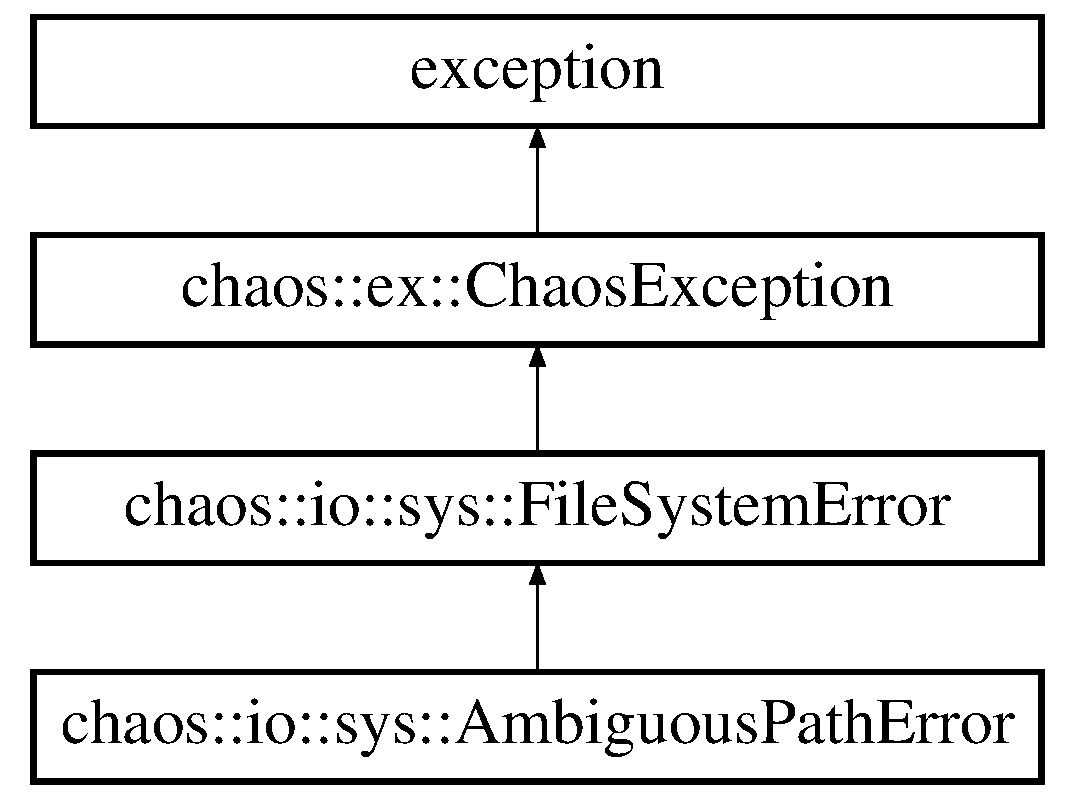
\includegraphics[height=4.000000cm]{classchaos_1_1io_1_1sys_1_1_ambiguous_path_error}
\end{center}
\end{figure}
\subsection*{Public Member Functions}
\begin{DoxyCompactItemize}
\item 
\hypertarget{classchaos_1_1io_1_1sys_1_1_ambiguous_path_error_a2c52d7f24bd88b11da5542f87b1b0bd9}{}{\bfseries Ambiguous\+Path\+Error} (const \hyperlink{classchaos_1_1uni_1_1_u_t_f8_string}{chaos\+::uni\+::\+U\+T\+F8\+String} \&message)\label{classchaos_1_1io_1_1sys_1_1_ambiguous_path_error_a2c52d7f24bd88b11da5542f87b1b0bd9}

\end{DoxyCompactItemize}
\subsection*{Additional Inherited Members}


\subsection{Detailed Description}
Warns that has a request has been made to create a file or directory that results in a ambiguous file system path. 

Example\+: a directory called \textquotesingle{}my\+\_\+name\textquotesingle{} was attempted to be created where a file also called \textquotesingle{}my\+\_\+name\textquotesingle{} already exists. 

The documentation for this class was generated from the following file\+:\begin{DoxyCompactItemize}
\item 
D\+:/\+Dropbox/\+Development/\+Chaos\+Core/\+Chaos\+Core/src/cxx/chaoscore/io/sys/\hyperlink{_file_system_exceptions_8hpp}{File\+System\+Exceptions.\+hpp}\end{DoxyCompactItemize}

\hypertarget{classchaos_1_1ex_1_1_arithmetic_error}{}\section{chaos\+:\+:ex\+:\+:Arithmetic\+Error Class Reference}
\label{classchaos_1_1ex_1_1_arithmetic_error}\index{chaos\+::ex\+::\+Arithmetic\+Error@{chaos\+::ex\+::\+Arithmetic\+Error}}


Warns of a failure due to bad arithmetic, e.\+g. zero division error.  




{\ttfamily \#include $<$Base\+Exceptions.\+hpp$>$}

Inheritance diagram for chaos\+:\+:ex\+:\+:Arithmetic\+Error\+:\begin{figure}[H]
\begin{center}
\leavevmode
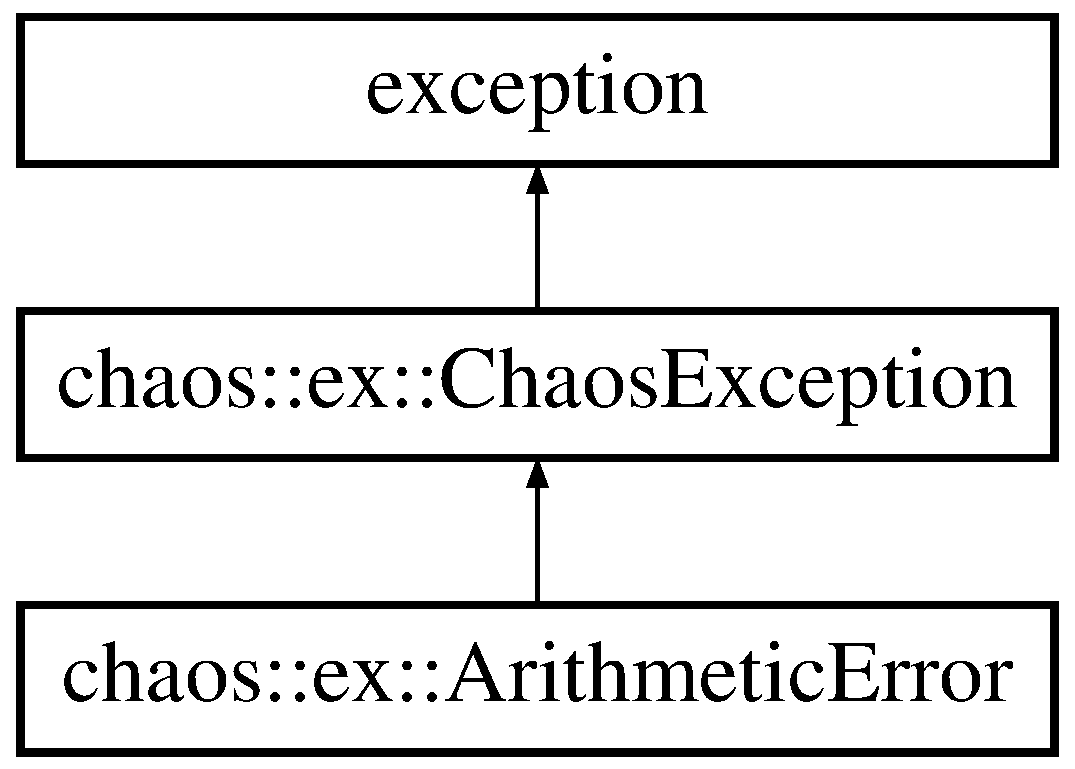
\includegraphics[height=3.000000cm]{classchaos_1_1ex_1_1_arithmetic_error}
\end{center}
\end{figure}
\subsection*{Public Member Functions}
\begin{DoxyCompactItemize}
\item 
\hypertarget{classchaos_1_1ex_1_1_arithmetic_error_a463d7850575f70f3d34d9db3300df29e}{}{\bfseries Arithmetic\+Error} (const \hyperlink{classchaos_1_1uni_1_1_u_t_f8_string}{chaos\+::uni\+::\+U\+T\+F8\+String} \&message)\label{classchaos_1_1ex_1_1_arithmetic_error_a463d7850575f70f3d34d9db3300df29e}

\end{DoxyCompactItemize}
\subsection*{Additional Inherited Members}


\subsection{Detailed Description}
Warns of a failure due to bad arithmetic, e.\+g. zero division error. 

The documentation for this class was generated from the following file\+:\begin{DoxyCompactItemize}
\item 
D\+:/\+Dropbox/\+Development/\+Chaos\+Core/\+Chaos\+Core/src/cxx/chaoscore/base/\hyperlink{_base_exceptions_8hpp}{Base\+Exceptions.\+hpp}\end{DoxyCompactItemize}

\hypertarget{unionchaos_1_1data_1_1_bitwise_float}{}\section{chaos\+:\+:data\+:\+:Bitwise\+Float Union Reference}
\label{unionchaos_1_1data_1_1_bitwise_float}\index{chaos\+::data\+::\+Bitwise\+Float@{chaos\+::data\+::\+Bitwise\+Float}}


Object that can be used to read and write the bits of a floating point number.  




{\ttfamily \#include $<$Bitwise\+Float.\+hpp$>$}

\subsection*{Public Member Functions}
\begin{DoxyCompactItemize}
\item 
\hyperlink{unionchaos_1_1data_1_1_bitwise_float_a7713ceaaa7cf2a487304088003d94135}{Bitwise\+Float} (float value)
\begin{DoxyCompactList}\small\item\em Float constructor. \end{DoxyCompactList}\item 
\hyperlink{unionchaos_1_1data_1_1_bitwise_float_a37070cb9a8ad9c96c709a2a08467ae77}{Bitwise\+Float} (const \hyperlink{unionchaos_1_1data_1_1_bitwise_float}{Bitwise\+Float} \&other)
\begin{DoxyCompactList}\small\item\em Copy constructor. \end{DoxyCompactList}\item 
\hyperlink{unionchaos_1_1data_1_1_bitwise_float}{Bitwise\+Float} \& \hyperlink{unionchaos_1_1data_1_1_bitwise_float_a2d2fdb0bfa06452e43184cb9a1db30f7}{operator=} (const \hyperlink{unionchaos_1_1data_1_1_bitwise_float}{Bitwise\+Float} \&other)
\begin{DoxyCompactList}\small\item\em Assignment operator. \end{DoxyCompactList}\item 
bool \hyperlink{unionchaos_1_1data_1_1_bitwise_float_a8c9504d5df1069a3b7af9bb1986dcab3}{operator==} (const \hyperlink{unionchaos_1_1data_1_1_bitwise_float}{Bitwise\+Float} \&other) const 
\begin{DoxyCompactList}\small\item\em Equality operator. \end{DoxyCompactList}\item 
bool \hyperlink{unionchaos_1_1data_1_1_bitwise_float_a103eeef1d692951938c2f269ea0accf3}{operator!=} (const \hyperlink{unionchaos_1_1data_1_1_bitwise_float}{Bitwise\+Float} \&other) const 
\begin{DoxyCompactList}\small\item\em Inequality operator. \end{DoxyCompactList}\item 
\hypertarget{unionchaos_1_1data_1_1_bitwise_float_aec1ad0a94dcf984131cc528b574c7d2d}{}bool \hyperlink{unionchaos_1_1data_1_1_bitwise_float_aec1ad0a94dcf984131cc528b574c7d2d}{get\+\_\+sign\+\_\+bit} () const \label{unionchaos_1_1data_1_1_bitwise_float_aec1ad0a94dcf984131cc528b574c7d2d}

\begin{DoxyCompactList}\small\item\em Retrieves the sign bit of this floating point number. \end{DoxyCompactList}\item 
\hypertarget{unionchaos_1_1data_1_1_bitwise_float_a53663822515d674b2fbcad78a758559c}{}void \hyperlink{unionchaos_1_1data_1_1_bitwise_float_a53663822515d674b2fbcad78a758559c}{set\+\_\+sign\+\_\+bit} (bool sign)\label{unionchaos_1_1data_1_1_bitwise_float_a53663822515d674b2fbcad78a758559c}

\begin{DoxyCompactList}\small\item\em Sets the sign bit (most significant bit) of this float. \end{DoxyCompactList}\item 
\hypertarget{unionchaos_1_1data_1_1_bitwise_float_a18da7f215f0f901943f24556cd9f1f4e}{}\hyperlink{namespacechaos_a8641b3ae4551f0b35570d4f9f4ec22d9}{chaos\+::uint32} \hyperlink{unionchaos_1_1data_1_1_bitwise_float_a18da7f215f0f901943f24556cd9f1f4e}{get\+\_\+exponent} () const \label{unionchaos_1_1data_1_1_bitwise_float_a18da7f215f0f901943f24556cd9f1f4e}

\begin{DoxyCompactList}\small\item\em Retrieves the 8-\/bit exponent section of this floating point number. \end{DoxyCompactList}\item 
\hypertarget{unionchaos_1_1data_1_1_bitwise_float_af3558e3752a224efb2b5e1b7df0ff473}{}void \hyperlink{unionchaos_1_1data_1_1_bitwise_float_af3558e3752a224efb2b5e1b7df0ff473}{set\+\_\+exponent} (\hyperlink{namespacechaos_acbc0796d6929e3182cfd4f5c0176ab51}{chaos\+::uint8} exponent)\label{unionchaos_1_1data_1_1_bitwise_float_af3558e3752a224efb2b5e1b7df0ff473}

\begin{DoxyCompactList}\small\item\em Sets the 8-\/bit exponent section of this floating point number. \end{DoxyCompactList}\item 
\hypertarget{unionchaos_1_1data_1_1_bitwise_float_afe4e313f09b01b6492a0dffce0d47b0b}{}\hyperlink{namespacechaos_a8641b3ae4551f0b35570d4f9f4ec22d9}{chaos\+::uint32} \hyperlink{unionchaos_1_1data_1_1_bitwise_float_afe4e313f09b01b6492a0dffce0d47b0b}{get\+\_\+mantissa} () const \label{unionchaos_1_1data_1_1_bitwise_float_afe4e313f09b01b6492a0dffce0d47b0b}

\begin{DoxyCompactList}\small\item\em Retrieves the 23-\/bit mantissa section of this floating point number. \end{DoxyCompactList}\item 
void \hyperlink{unionchaos_1_1data_1_1_bitwise_float_a57629a8a0c7aaff58ba05bcab7831ce6}{set\+\_\+mantissa} (\hyperlink{namespacechaos_a8641b3ae4551f0b35570d4f9f4ec22d9}{chaos\+::uint32} mantissa)
\begin{DoxyCompactList}\small\item\em Sets the 23-\/bit mantissa section of this floating point number. \end{DoxyCompactList}\item 
float \hyperlink{unionchaos_1_1data_1_1_bitwise_float_ab38870254ea2295c45556e9aa51c2554}{precision\+\_\+away\+\_\+from\+\_\+zero} () const 
\begin{DoxyCompactList}\small\item\em Returns the precision of this float away from zero. \end{DoxyCompactList}\item 
float \hyperlink{unionchaos_1_1data_1_1_bitwise_float_a4acc915134b0cdab21c6e3c30842754d}{precision\+\_\+towards\+\_\+zero} () const 
\begin{DoxyCompactList}\small\item\em Returns the precision of this float away from zero. \end{DoxyCompactList}\end{DoxyCompactItemize}
\subsection*{Public Attributes}
\begin{DoxyCompactItemize}
\item 
\hypertarget{unionchaos_1_1data_1_1_bitwise_float_ab763103c6f0079798d187c8c27612259}{}float \hyperlink{unionchaos_1_1data_1_1_bitwise_float_ab763103c6f0079798d187c8c27612259}{float\+\_\+rep}\label{unionchaos_1_1data_1_1_bitwise_float_ab763103c6f0079798d187c8c27612259}

\begin{DoxyCompactList}\small\item\em Access to the float representation. \end{DoxyCompactList}\item 
\hypertarget{unionchaos_1_1data_1_1_bitwise_float_a5dc7a9d68bc17cecceec14da1ac9b592}{}\hyperlink{namespacechaos_a8641b3ae4551f0b35570d4f9f4ec22d9}{chaos\+::uint32} \hyperlink{unionchaos_1_1data_1_1_bitwise_float_a5dc7a9d68bc17cecceec14da1ac9b592}{int\+\_\+rep}\label{unionchaos_1_1data_1_1_bitwise_float_a5dc7a9d68bc17cecceec14da1ac9b592}

\begin{DoxyCompactList}\small\item\em Access to the int representation. \end{DoxyCompactList}\end{DoxyCompactItemize}


\subsection{Detailed Description}
Object that can be used to read and write the bits of a floating point number. 

Floating point numbers are composed of three sections\+: sign, exponent, and mantissa. These sections are laid out like so\+:


\begin{DoxyCode}
0 00000000 00000000000000000000000
^ \(\backslash\)------/ \(\backslash\)---------------------/
|     |                |
\(\backslash\) 8-bit exponent       |
 \(\backslash\)                23-bit mantissa
sign bit
\end{DoxyCode}


This object provides functions for reading and writing these sections of a floating point number. 

\subsection{Constructor \& Destructor Documentation}
\hypertarget{unionchaos_1_1data_1_1_bitwise_float_a7713ceaaa7cf2a487304088003d94135}{}\index{chaos\+::data\+::\+Bitwise\+Float@{chaos\+::data\+::\+Bitwise\+Float}!Bitwise\+Float@{Bitwise\+Float}}
\index{Bitwise\+Float@{Bitwise\+Float}!chaos\+::data\+::\+Bitwise\+Float@{chaos\+::data\+::\+Bitwise\+Float}}
\subsubsection[{Bitwise\+Float(float value)}]{\setlength{\rightskip}{0pt plus 5cm}chaos\+::data\+::\+Bitwise\+Float\+::\+Bitwise\+Float (
\begin{DoxyParamCaption}
\item[{float}]{value}
\end{DoxyParamCaption}
)}\label{unionchaos_1_1data_1_1_bitwise_float_a7713ceaaa7cf2a487304088003d94135}


Float constructor. 

Creates a new Bitewise\+Float initialised with the given value. \hypertarget{unionchaos_1_1data_1_1_bitwise_float_a37070cb9a8ad9c96c709a2a08467ae77}{}\index{chaos\+::data\+::\+Bitwise\+Float@{chaos\+::data\+::\+Bitwise\+Float}!Bitwise\+Float@{Bitwise\+Float}}
\index{Bitwise\+Float@{Bitwise\+Float}!chaos\+::data\+::\+Bitwise\+Float@{chaos\+::data\+::\+Bitwise\+Float}}
\subsubsection[{Bitwise\+Float(const Bitwise\+Float \&other)}]{\setlength{\rightskip}{0pt plus 5cm}chaos\+::data\+::\+Bitwise\+Float\+::\+Bitwise\+Float (
\begin{DoxyParamCaption}
\item[{const {\bf Bitwise\+Float} \&}]{other}
\end{DoxyParamCaption}
)}\label{unionchaos_1_1data_1_1_bitwise_float_a37070cb9a8ad9c96c709a2a08467ae77}


Copy constructor. 

Creates a copy of the other given \hyperlink{unionchaos_1_1data_1_1_bitwise_float}{Bitwise\+Float}. 

\subsection{Member Function Documentation}
\hypertarget{unionchaos_1_1data_1_1_bitwise_float_a2d2fdb0bfa06452e43184cb9a1db30f7}{}\index{chaos\+::data\+::\+Bitwise\+Float@{chaos\+::data\+::\+Bitwise\+Float}!operator=@{operator=}}
\index{operator=@{operator=}!chaos\+::data\+::\+Bitwise\+Float@{chaos\+::data\+::\+Bitwise\+Float}}
\subsubsection[{operator=(const Bitwise\+Float \&other)}]{\setlength{\rightskip}{0pt plus 5cm}{\bf Bitwise\+Float}\& chaos\+::data\+::\+Bitwise\+Float\+::operator= (
\begin{DoxyParamCaption}
\item[{const {\bf Bitwise\+Float} \&}]{other}
\end{DoxyParamCaption}
)}\label{unionchaos_1_1data_1_1_bitwise_float_a2d2fdb0bfa06452e43184cb9a1db30f7}


Assignment operator. 

Assigns the value of this \hyperlink{unionchaos_1_1data_1_1_bitwise_float}{Bitwise\+Float} to be a copy of the value of the other given \hyperlink{unionchaos_1_1data_1_1_bitwise_float}{Bitwise\+Float}.


\begin{DoxyParams}{Parameters}
{\em other} & \hyperlink{unionchaos_1_1data_1_1_bitwise_float}{Bitwise\+Float} to copy from. \\
\hline
\end{DoxyParams}
\begin{DoxyReturn}{Returns}
A reference to this \hyperlink{unionchaos_1_1data_1_1_bitwise_float}{Bitwise\+Float} once the assignment has taken place. 
\end{DoxyReturn}
\hypertarget{unionchaos_1_1data_1_1_bitwise_float_a8c9504d5df1069a3b7af9bb1986dcab3}{}\index{chaos\+::data\+::\+Bitwise\+Float@{chaos\+::data\+::\+Bitwise\+Float}!operator==@{operator==}}
\index{operator==@{operator==}!chaos\+::data\+::\+Bitwise\+Float@{chaos\+::data\+::\+Bitwise\+Float}}
\subsubsection[{operator==(const Bitwise\+Float \&other) const }]{\setlength{\rightskip}{0pt plus 5cm}bool chaos\+::data\+::\+Bitwise\+Float\+::operator== (
\begin{DoxyParamCaption}
\item[{const {\bf Bitwise\+Float} \&}]{other}
\end{DoxyParamCaption}
) const}\label{unionchaos_1_1data_1_1_bitwise_float_a8c9504d5df1069a3b7af9bb1986dcab3}


Equality operator. 

Compares whether this \hyperlink{unionchaos_1_1data_1_1_bitwise_float}{Bitwise\+Float} and the other \hyperlink{unionchaos_1_1data_1_1_bitwise_float}{Bitwise\+Float} are considered equal.

Equality is defined by a comparison of the exact \hyperlink{unionchaos_1_1data_1_1_bitwise_float_a5dc7a9d68bc17cecceec14da1ac9b592}{Bitwise\+Float.\+int\+\_\+rep} values.

For more flexible floating point comparisons see chaos\+::math\+::float\+\_\+equals(). \hypertarget{unionchaos_1_1data_1_1_bitwise_float_a103eeef1d692951938c2f269ea0accf3}{}\index{chaos\+::data\+::\+Bitwise\+Float@{chaos\+::data\+::\+Bitwise\+Float}!operator"!=@{operator"!=}}
\index{operator"!=@{operator"!=}!chaos\+::data\+::\+Bitwise\+Float@{chaos\+::data\+::\+Bitwise\+Float}}
\subsubsection[{operator"!=(const Bitwise\+Float \&other) const }]{\setlength{\rightskip}{0pt plus 5cm}bool chaos\+::data\+::\+Bitwise\+Float\+::operator!= (
\begin{DoxyParamCaption}
\item[{const {\bf Bitwise\+Float} \&}]{other}
\end{DoxyParamCaption}
) const}\label{unionchaos_1_1data_1_1_bitwise_float_a103eeef1d692951938c2f269ea0accf3}


Inequality operator. 

Compares whether this \hyperlink{unionchaos_1_1data_1_1_bitwise_float}{Bitwise\+Float} and the other \hyperlink{unionchaos_1_1data_1_1_bitwise_float}{Bitwise\+Float} are considered not equal.

Equality is defined by a comparison of the exact \hyperlink{unionchaos_1_1data_1_1_bitwise_float_a5dc7a9d68bc17cecceec14da1ac9b592}{Bitwise\+Float.\+int\+\_\+rep} values.

For more flexible floating point comparisons see chaos\+::math\+::float\+\_\+equals(). \hypertarget{unionchaos_1_1data_1_1_bitwise_float_a57629a8a0c7aaff58ba05bcab7831ce6}{}\index{chaos\+::data\+::\+Bitwise\+Float@{chaos\+::data\+::\+Bitwise\+Float}!set\+\_\+mantissa@{set\+\_\+mantissa}}
\index{set\+\_\+mantissa@{set\+\_\+mantissa}!chaos\+::data\+::\+Bitwise\+Float@{chaos\+::data\+::\+Bitwise\+Float}}
\subsubsection[{set\+\_\+mantissa(chaos\+::uint32 mantissa)}]{\setlength{\rightskip}{0pt plus 5cm}void chaos\+::data\+::\+Bitwise\+Float\+::set\+\_\+mantissa (
\begin{DoxyParamCaption}
\item[{{\bf chaos\+::uint32}}]{mantissa}
\end{DoxyParamCaption}
)}\label{unionchaos_1_1data_1_1_bitwise_float_a57629a8a0c7aaff58ba05bcab7831ce6}


Sets the 23-\/bit mantissa section of this floating point number. 

\begin{DoxyNote}{Note}
While a 32-\/bit input value is accepted only the least significant 23-\/bits of this value will be used. 
\end{DoxyNote}
\hypertarget{unionchaos_1_1data_1_1_bitwise_float_ab38870254ea2295c45556e9aa51c2554}{}\index{chaos\+::data\+::\+Bitwise\+Float@{chaos\+::data\+::\+Bitwise\+Float}!precision\+\_\+away\+\_\+from\+\_\+zero@{precision\+\_\+away\+\_\+from\+\_\+zero}}
\index{precision\+\_\+away\+\_\+from\+\_\+zero@{precision\+\_\+away\+\_\+from\+\_\+zero}!chaos\+::data\+::\+Bitwise\+Float@{chaos\+::data\+::\+Bitwise\+Float}}
\subsubsection[{precision\+\_\+away\+\_\+from\+\_\+zero() const }]{\setlength{\rightskip}{0pt plus 5cm}float chaos\+::data\+::\+Bitwise\+Float\+::precision\+\_\+away\+\_\+from\+\_\+zero (
\begin{DoxyParamCaption}
{}
\end{DoxyParamCaption}
) const}\label{unionchaos_1_1data_1_1_bitwise_float_ab38870254ea2295c45556e9aa51c2554}


Returns the precision of this float away from zero. 

Floating point precision is measured as the difference between this number and the next possible float value away from zero.


\begin{DoxyExceptions}{Exceptions}
{\em \hyperlink{classchaos_1_1ex_1_1_arithmetic_error}{chaos\+::ex\+::\+Arithmetic\+Error}} & If this float is infinity or Na\+N. \\
\hline
\end{DoxyExceptions}
\hypertarget{unionchaos_1_1data_1_1_bitwise_float_a4acc915134b0cdab21c6e3c30842754d}{}\index{chaos\+::data\+::\+Bitwise\+Float@{chaos\+::data\+::\+Bitwise\+Float}!precision\+\_\+towards\+\_\+zero@{precision\+\_\+towards\+\_\+zero}}
\index{precision\+\_\+towards\+\_\+zero@{precision\+\_\+towards\+\_\+zero}!chaos\+::data\+::\+Bitwise\+Float@{chaos\+::data\+::\+Bitwise\+Float}}
\subsubsection[{precision\+\_\+towards\+\_\+zero() const }]{\setlength{\rightskip}{0pt plus 5cm}float chaos\+::data\+::\+Bitwise\+Float\+::precision\+\_\+towards\+\_\+zero (
\begin{DoxyParamCaption}
{}
\end{DoxyParamCaption}
) const}\label{unionchaos_1_1data_1_1_bitwise_float_a4acc915134b0cdab21c6e3c30842754d}


Returns the precision of this float away from zero. 

Floating point precision is measured as the difference between this number and the next possible float value towards zero.


\begin{DoxyExceptions}{Exceptions}
{\em \hyperlink{classchaos_1_1ex_1_1_arithmetic_error}{chaos\+::ex\+::\+Arithmetic\+Error}} & If this float is 0 or Na\+N. \\
\hline
\end{DoxyExceptions}


The documentation for this union was generated from the following file\+:\begin{DoxyCompactItemize}
\item 
D\+:/\+Dropbox/\+Development/\+Chaos\+Core/\+Chaos\+Core/src/cxx/chaoscore/base/data/Bitwise\+Float.\+hpp\end{DoxyCompactItemize}

\hypertarget{classchaos_1_1ex_1_1_chaos_exception}{}\section{chaos\+:\+:ex\+:\+:Chaos\+Exception Class Reference}
\label{classchaos_1_1ex_1_1_chaos_exception}\index{chaos\+::ex\+::\+Chaos\+Exception@{chaos\+::ex\+::\+Chaos\+Exception}}


Abstract base class that all Chaos\+Core Exceptions extend from.  




{\ttfamily \#include $<$Base\+Exceptions.\+hpp$>$}

Inheritance diagram for chaos\+:\+:ex\+:\+:Chaos\+Exception\+:\begin{figure}[H]
\begin{center}
\leavevmode
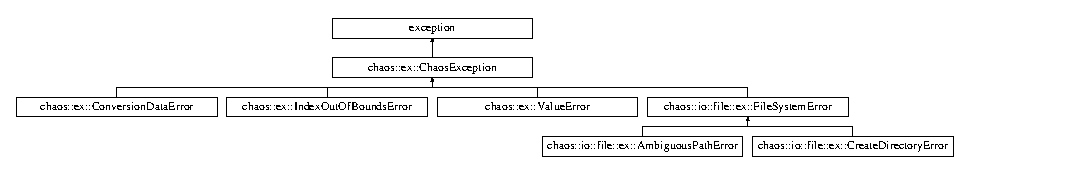
\includegraphics[height=1.171548cm]{classchaos_1_1ex_1_1_chaos_exception}
\end{center}
\end{figure}
\subsection*{Public Member Functions}
\begin{DoxyCompactItemize}
\item 
virtual const char $\ast$ \hyperlink{classchaos_1_1ex_1_1_chaos_exception_a5266c5ba1e7b6ab2bbfcb2a6c01fafea}{what} () const   throw ()
\item 
const \hyperlink{classchaos_1_1uni_1_1_u_t_f8_string}{chaos\+::uni\+::\+U\+T\+F8\+String} \& \hyperlink{classchaos_1_1ex_1_1_chaos_exception_a03cf7cf992d411770c7cefa925c84f4f}{get\+\_\+message} () const 
\end{DoxyCompactItemize}
\subsection*{Protected Member Functions}
\begin{DoxyCompactItemize}
\item 
\hyperlink{classchaos_1_1ex_1_1_chaos_exception_a66463bad3b8d75073ae73c27717ae70d}{Chaos\+Exception} (const \hyperlink{classchaos_1_1uni_1_1_u_t_f8_string}{chaos\+::uni\+::\+U\+T\+F8\+String} \&message)
\begin{DoxyCompactList}\small\item\em Super constructor for objects derived from \hyperlink{classchaos_1_1ex_1_1_chaos_exception}{Chaos\+Exception}. \end{DoxyCompactList}\end{DoxyCompactItemize}


\subsection{Detailed Description}
Abstract base class that all Chaos\+Core Exceptions extend from. 

This class directly inherits from std\+::exception. 

\subsection{Constructor \& Destructor Documentation}
\hypertarget{classchaos_1_1ex_1_1_chaos_exception_a66463bad3b8d75073ae73c27717ae70d}{}\index{chaos\+::ex\+::\+Chaos\+Exception@{chaos\+::ex\+::\+Chaos\+Exception}!Chaos\+Exception@{Chaos\+Exception}}
\index{Chaos\+Exception@{Chaos\+Exception}!chaos\+::ex\+::\+Chaos\+Exception@{chaos\+::ex\+::\+Chaos\+Exception}}
\subsubsection[{Chaos\+Exception(const chaos\+::uni\+::\+U\+T\+F8\+String \&message)}]{\setlength{\rightskip}{0pt plus 5cm}chaos\+::ex\+::\+Chaos\+Exception\+::\+Chaos\+Exception (
\begin{DoxyParamCaption}
\item[{const {\bf chaos\+::uni\+::\+U\+T\+F8\+String} \&}]{message}
\end{DoxyParamCaption}
)\hspace{0.3cm}{\ttfamily [inline]}, {\ttfamily [protected]}}\label{classchaos_1_1ex_1_1_chaos_exception_a66463bad3b8d75073ae73c27717ae70d}


Super constructor for objects derived from \hyperlink{classchaos_1_1ex_1_1_chaos_exception}{Chaos\+Exception}. 


\begin{DoxyParams}{Parameters}
{\em message} & A message decribing the reason for the exception. \\
\hline
\end{DoxyParams}


\subsection{Member Function Documentation}
\hypertarget{classchaos_1_1ex_1_1_chaos_exception_a5266c5ba1e7b6ab2bbfcb2a6c01fafea}{}\index{chaos\+::ex\+::\+Chaos\+Exception@{chaos\+::ex\+::\+Chaos\+Exception}!what@{what}}
\index{what@{what}!chaos\+::ex\+::\+Chaos\+Exception@{chaos\+::ex\+::\+Chaos\+Exception}}
\subsubsection[{what() const }]{\setlength{\rightskip}{0pt plus 5cm}virtual const char$\ast$ chaos\+::ex\+::\+Chaos\+Exception\+::what (
\begin{DoxyParamCaption}
{}
\end{DoxyParamCaption}
) const throw  ) \hspace{0.3cm}{\ttfamily [inline]}, {\ttfamily [virtual]}}\label{classchaos_1_1ex_1_1_chaos_exception_a5266c5ba1e7b6ab2bbfcb2a6c01fafea}
\begin{DoxyReturn}{Returns}
The reason for the exception. 
\end{DoxyReturn}
\hypertarget{classchaos_1_1ex_1_1_chaos_exception_a03cf7cf992d411770c7cefa925c84f4f}{}\index{chaos\+::ex\+::\+Chaos\+Exception@{chaos\+::ex\+::\+Chaos\+Exception}!get\+\_\+message@{get\+\_\+message}}
\index{get\+\_\+message@{get\+\_\+message}!chaos\+::ex\+::\+Chaos\+Exception@{chaos\+::ex\+::\+Chaos\+Exception}}
\subsubsection[{get\+\_\+message() const }]{\setlength{\rightskip}{0pt plus 5cm}const {\bf chaos\+::uni\+::\+U\+T\+F8\+String}\& chaos\+::ex\+::\+Chaos\+Exception\+::get\+\_\+message (
\begin{DoxyParamCaption}
{}
\end{DoxyParamCaption}
) const\hspace{0.3cm}{\ttfamily [inline]}}\label{classchaos_1_1ex_1_1_chaos_exception_a03cf7cf992d411770c7cefa925c84f4f}
\begin{DoxyReturn}{Returns}
The reason for the exception. 
\end{DoxyReturn}


The documentation for this class was generated from the following file\+:\begin{DoxyCompactItemize}
\item 
D\+:/\+Dropbox/\+Development/\+Chaos\+Core/\+Chaos\+Core/src/cxx/chaoscore/base/\hyperlink{_base_exceptions_8hpp}{Base\+Exceptions.\+hpp}\end{DoxyCompactItemize}

\hypertarget{classchaos_1_1ex_1_1_conversion_data_error}{}\section{chaos\+:\+:ex\+:\+:Conversion\+Data\+Error Class Reference}
\label{classchaos_1_1ex_1_1_conversion_data_error}\index{chaos\+::ex\+::\+Conversion\+Data\+Error@{chaos\+::ex\+::\+Conversion\+Data\+Error}}


Warns that the provided data for a type conversion was bad or invalid.  




{\ttfamily \#include $<$Base\+Exceptions.\+hpp$>$}

Inheritance diagram for chaos\+:\+:ex\+:\+:Conversion\+Data\+Error\+:\begin{figure}[H]
\begin{center}
\leavevmode
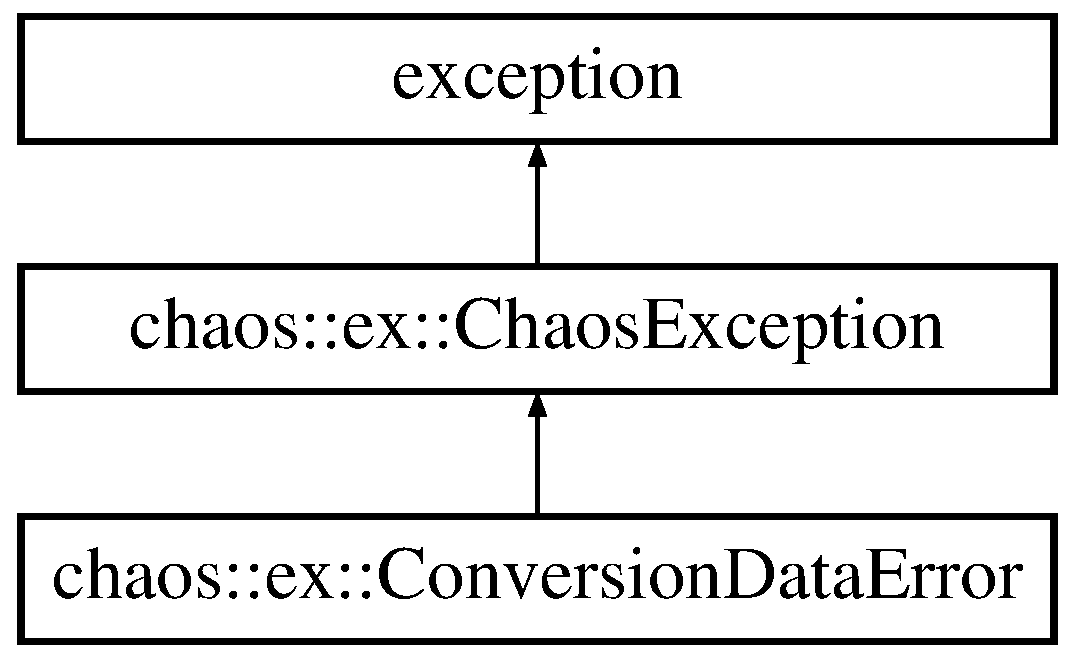
\includegraphics[height=3.000000cm]{classchaos_1_1ex_1_1_conversion_data_error}
\end{center}
\end{figure}
\subsection*{Public Member Functions}
\begin{DoxyCompactItemize}
\item 
\hypertarget{classchaos_1_1ex_1_1_conversion_data_error_afef7fd90707b2bd0be147090613c1222}{}{\bfseries Conversion\+Data\+Error} (const \hyperlink{classchaos_1_1str_1_1_u_t_f8_string}{chaos\+::str\+::\+U\+T\+F8\+String} \&message)\label{classchaos_1_1ex_1_1_conversion_data_error_afef7fd90707b2bd0be147090613c1222}

\end{DoxyCompactItemize}
\subsection*{Additional Inherited Members}


\subsection{Detailed Description}
Warns that the provided data for a type conversion was bad or invalid. 

The documentation for this class was generated from the following file\+:\begin{DoxyCompactItemize}
\item 
D\+:/\+Dropbox/\+Development/\+Chaos\+Core/\+Chaos\+Core/src/cxx/chaoscore/base/\hyperlink{_base_exceptions_8hpp}{Base\+Exceptions.\+hpp}\end{DoxyCompactItemize}

\hypertarget{classchaos_1_1io_1_1sys_1_1_create_directory_error}{\section{chaos\-:\-:io\-:\-:sys\-:\-:Create\-Directory\-Error Class Reference}
\label{classchaos_1_1io_1_1sys_1_1_create_directory_error}\index{chaos\-::io\-::sys\-::\-Create\-Directory\-Error@{chaos\-::io\-::sys\-::\-Create\-Directory\-Error}}
}


Warns that creating a directory has failed.  




{\ttfamily \#include $<$File\-System\-Exceptions.\-hpp$>$}

Inheritance diagram for chaos\-:\-:io\-:\-:sys\-:\-:Create\-Directory\-Error\-:\begin{figure}[H]
\begin{center}
\leavevmode
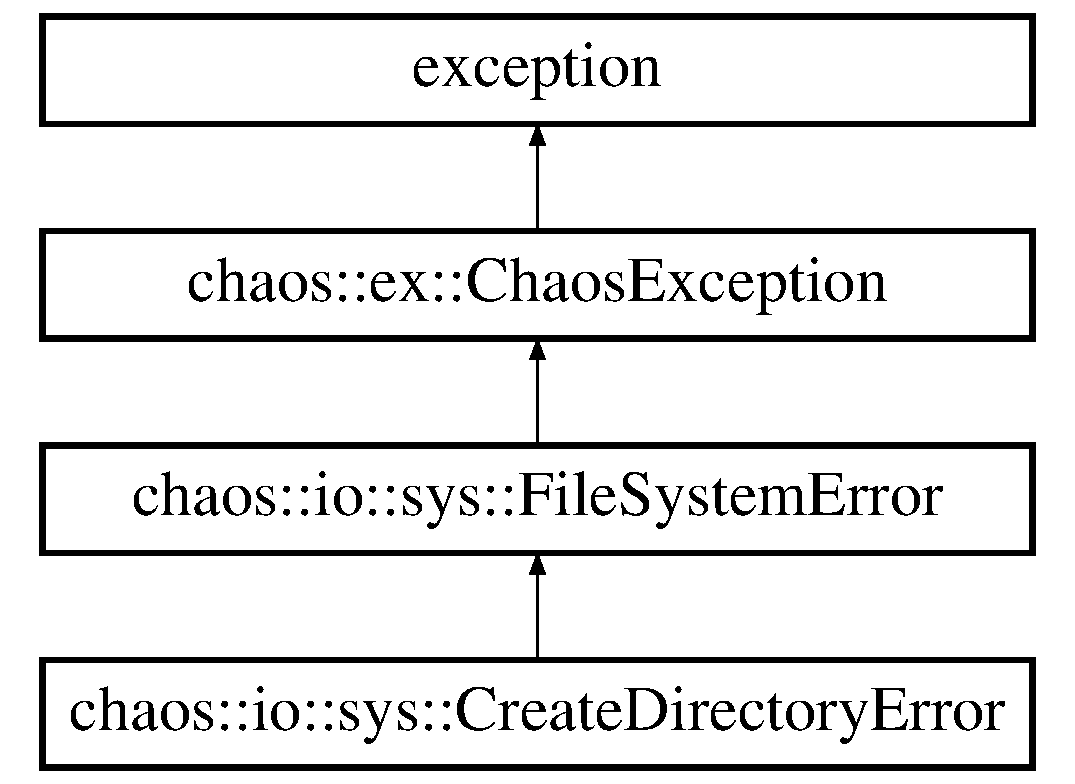
\includegraphics[height=4.000000cm]{classchaos_1_1io_1_1sys_1_1_create_directory_error}
\end{center}
\end{figure}
\subsection*{Public Member Functions}
\begin{DoxyCompactItemize}
\item 
\hypertarget{classchaos_1_1io_1_1sys_1_1_create_directory_error_aab9a24330c9607be0391dbbe08149fcf}{{\bfseries Create\-Directory\-Error} (const \hyperlink{classchaos_1_1uni_1_1_u_t_f8_string}{chaos\-::uni\-::\-U\-T\-F8\-String} \&message)}\label{classchaos_1_1io_1_1sys_1_1_create_directory_error_aab9a24330c9607be0391dbbe08149fcf}

\end{DoxyCompactItemize}
\subsection*{Additional Inherited Members}


\subsection{Detailed Description}
Warns that creating a directory has failed. 

The documentation for this class was generated from the following file\-:\begin{DoxyCompactItemize}
\item 
/home/david/\-Dropbox/\-Development/\-Chaos\-Core/\-Chaos\-Core/src/cxx/chaoscore/io/sys/\hyperlink{_file_system_exceptions_8hpp}{File\-System\-Exceptions.\-hpp}\end{DoxyCompactItemize}

\hypertarget{classchaos_1_1io_1_1sys_1_1_file_handle}{}\section{chaos\+:\+:io\+:\+:sys\+:\+:File\+Handle Class Reference}
\label{classchaos_1_1io_1_1sys_1_1_file_handle}\index{chaos\+::io\+::sys\+::\+File\+Handle@{chaos\+::io\+::sys\+::\+File\+Handle}}


Abstract base class used for representing an object that is writing or reading to/from a file.  




{\ttfamily \#include $<$File\+Handle.\+hpp$>$}

Inheritance diagram for chaos\+:\+:io\+:\+:sys\+:\+:File\+Handle\+:\begin{figure}[H]
\begin{center}
\leavevmode
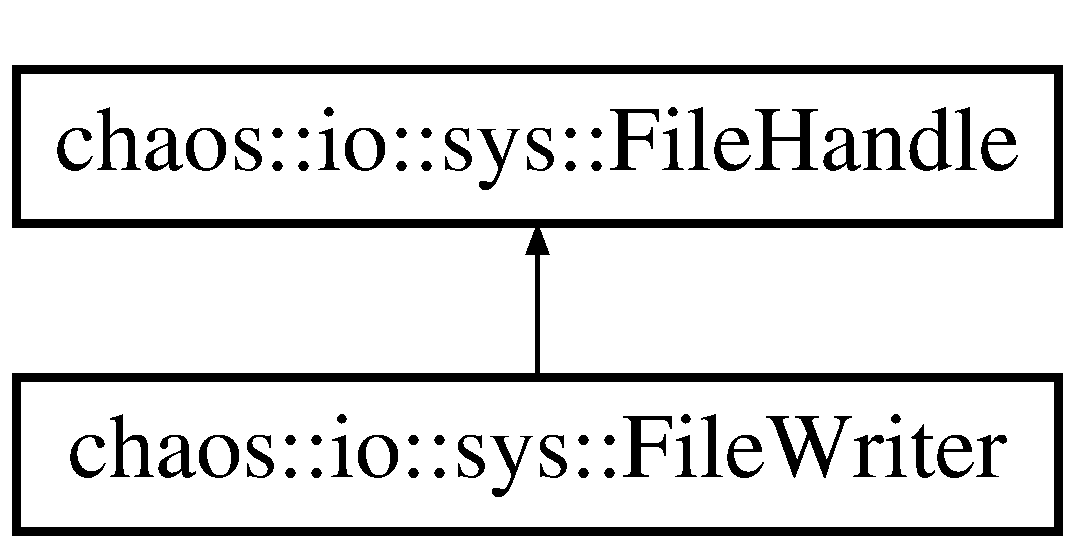
\includegraphics[height=2.000000cm]{classchaos_1_1io_1_1sys_1_1_file_handle}
\end{center}
\end{figure}
\subsection*{Public Member Functions}
\begin{DoxyCompactItemize}
\item 
virtual void \hyperlink{classchaos_1_1io_1_1sys_1_1_file_handle_aaab721e850f11cd1f1bf3dba8e4ab2a1}{open} ()=0
\begin{DoxyCompactList}\small\item\em Opens the file handle to the internal path. \end{DoxyCompactList}\item 
virtual void \hyperlink{classchaos_1_1io_1_1sys_1_1_file_handle_ac38cdc6e3d48bba2d6e143265c7aaaad}{open} (const \hyperlink{classchaos_1_1io_1_1sys_1_1_path}{chaos\+::io\+::sys\+::\+Path} \&path)
\begin{DoxyCompactList}\small\item\em Sets the path and opens this handle to it. \end{DoxyCompactList}\item 
virtual void \hyperlink{classchaos_1_1io_1_1sys_1_1_file_handle_ac4dd796f7080d16fd2b141806e23f004}{close} ()=0
\begin{DoxyCompactList}\small\item\em Closes this file handle. \end{DoxyCompactList}\item 
\hypertarget{classchaos_1_1io_1_1sys_1_1_file_handle_aeb0c8615f3b16ceb7f9130b1482b3b42}{}virtual const \hyperlink{classchaos_1_1io_1_1sys_1_1_path}{chaos\+::io\+::sys\+::\+Path} \& \hyperlink{classchaos_1_1io_1_1sys_1_1_file_handle_aeb0c8615f3b16ceb7f9130b1482b3b42}{get\+\_\+path} () const \label{classchaos_1_1io_1_1sys_1_1_file_handle_aeb0c8615f3b16ceb7f9130b1482b3b42}

\begin{DoxyCompactList}\small\item\em Returns the path being used by this file handle. \end{DoxyCompactList}\item 
virtual void \hyperlink{classchaos_1_1io_1_1sys_1_1_file_handle_a14272fcf341c329bf15f7198b5e08573}{set\+\_\+path} (const \hyperlink{classchaos_1_1io_1_1sys_1_1_path}{chaos\+::io\+::sys\+::\+Path} \&path)
\begin{DoxyCompactList}\small\item\em Sets the path to be used by this file handle. \end{DoxyCompactList}\item 
\hypertarget{classchaos_1_1io_1_1sys_1_1_file_handle_a5cfd6d2ef58b86bf4a8b729a0825f508}{}virtual \hyperlink{namespacechaos_a8641b3ae4551f0b35570d4f9f4ec22d9}{chaos\+::uint32} \hyperlink{classchaos_1_1io_1_1sys_1_1_file_handle_a5cfd6d2ef58b86bf4a8b729a0825f508}{get\+\_\+flags} () const \label{classchaos_1_1io_1_1sys_1_1_file_handle_a5cfd6d2ef58b86bf4a8b729a0825f508}

\begin{DoxyCompactList}\small\item\em Returns the descriptor flags of the this file handle. \end{DoxyCompactList}\item 
virtual void \hyperlink{classchaos_1_1io_1_1sys_1_1_file_handle_a8ad8c2176597a8c56e38a3bd51b1c7dd}{set\+\_\+flags} (\hyperlink{namespacechaos_a8641b3ae4551f0b35570d4f9f4ec22d9}{chaos\+::uint32} flags)
\begin{DoxyCompactList}\small\item\em Sets the descriptor flags to be used by this file handle. \end{DoxyCompactList}\end{DoxyCompactItemize}
\subsection*{Protected Member Functions}
\begin{DoxyCompactItemize}
\item 
\hyperlink{classchaos_1_1io_1_1sys_1_1_file_handle_af5d96eae217fa6b8f770ba614b4beeaa}{File\+Handle} (\hyperlink{namespacechaos_a8641b3ae4551f0b35570d4f9f4ec22d9}{chaos\+::uint32} flags=0\+U)
\begin{DoxyCompactList}\small\item\em Default super constructor. \end{DoxyCompactList}\item 
\hyperlink{classchaos_1_1io_1_1sys_1_1_file_handle_ac27707755a7e9ab9390ee3ed50db9c3c}{File\+Handle} (const \hyperlink{classchaos_1_1io_1_1sys_1_1_path}{chaos\+::io\+::sys\+::\+Path} \&path, \hyperlink{namespacechaos_a8641b3ae4551f0b35570d4f9f4ec22d9}{chaos\+::uint32} flags=0\+U)
\begin{DoxyCompactList}\small\item\em \hyperlink{classchaos_1_1io_1_1sys_1_1_path}{Path} super constructor. \end{DoxyCompactList}\end{DoxyCompactItemize}
\subsection*{Protected Attributes}
\begin{DoxyCompactItemize}
\item 
\hypertarget{classchaos_1_1io_1_1sys_1_1_file_handle_a8e6a9c9ab7d7abec8fc2bbcf595cfba1}{}\hyperlink{classchaos_1_1io_1_1sys_1_1_path}{chaos\+::io\+::sys\+::\+Path} \hyperlink{classchaos_1_1io_1_1sys_1_1_file_handle_a8e6a9c9ab7d7abec8fc2bbcf595cfba1}{m\+\_\+path}\label{classchaos_1_1io_1_1sys_1_1_file_handle_a8e6a9c9ab7d7abec8fc2bbcf595cfba1}

\begin{DoxyCompactList}\small\item\em The file path this handle is currently using. \end{DoxyCompactList}\item 
\hypertarget{classchaos_1_1io_1_1sys_1_1_file_handle_aa6a2c99d5e0b94ed1d9c4b511352f78a}{}\hyperlink{namespacechaos_a8641b3ae4551f0b35570d4f9f4ec22d9}{chaos\+::uint32} \hyperlink{classchaos_1_1io_1_1sys_1_1_file_handle_aa6a2c99d5e0b94ed1d9c4b511352f78a}{m\+\_\+flags}\label{classchaos_1_1io_1_1sys_1_1_file_handle_aa6a2c99d5e0b94ed1d9c4b511352f78a}

\begin{DoxyCompactList}\small\item\em Descriptor flags of the file handle. \end{DoxyCompactList}\item 
\hypertarget{classchaos_1_1io_1_1sys_1_1_file_handle_a4047ce2fadb3410ce99b5869da16007d}{}bool \hyperlink{classchaos_1_1io_1_1sys_1_1_file_handle_a4047ce2fadb3410ce99b5869da16007d}{m\+\_\+open}\label{classchaos_1_1io_1_1sys_1_1_file_handle_a4047ce2fadb3410ce99b5869da16007d}

\begin{DoxyCompactList}\small\item\em Whether the file handle is currently open or not. \end{DoxyCompactList}\end{DoxyCompactItemize}


\subsection{Detailed Description}
Abstract base class used for representing an object that is writing or reading to/from a file. 

This object defines the specifications for chaos\+::io\+::sys\+::\+File\+Reader and \hyperlink{classchaos_1_1io_1_1sys_1_1_file_writer}{chaos\+::io\+::sys\+::\+File\+Writer}. 

\subsection{Constructor \& Destructor Documentation}
\hypertarget{classchaos_1_1io_1_1sys_1_1_file_handle_af5d96eae217fa6b8f770ba614b4beeaa}{}\index{chaos\+::io\+::sys\+::\+File\+Handle@{chaos\+::io\+::sys\+::\+File\+Handle}!File\+Handle@{File\+Handle}}
\index{File\+Handle@{File\+Handle}!chaos\+::io\+::sys\+::\+File\+Handle@{chaos\+::io\+::sys\+::\+File\+Handle}}
\subsubsection[{File\+Handle(chaos\+::uint32 flags=0\+U)}]{\setlength{\rightskip}{0pt plus 5cm}chaos\+::io\+::sys\+::\+File\+Handle\+::\+File\+Handle (
\begin{DoxyParamCaption}
\item[{{\bf chaos\+::uint32}}]{flags = {\ttfamily 0U}}
\end{DoxyParamCaption}
)\hspace{0.3cm}{\ttfamily [protected]}}\label{classchaos_1_1io_1_1sys_1_1_file_handle_af5d96eae217fa6b8f770ba614b4beeaa}


Default super constructor. 

Super constructor used to create a new unopened file handle.


\begin{DoxyParams}{Parameters}
{\em flags} & Flags used to describe how the file handle should be opened. \\
\hline
\end{DoxyParams}
\hypertarget{classchaos_1_1io_1_1sys_1_1_file_handle_ac27707755a7e9ab9390ee3ed50db9c3c}{}\index{chaos\+::io\+::sys\+::\+File\+Handle@{chaos\+::io\+::sys\+::\+File\+Handle}!File\+Handle@{File\+Handle}}
\index{File\+Handle@{File\+Handle}!chaos\+::io\+::sys\+::\+File\+Handle@{chaos\+::io\+::sys\+::\+File\+Handle}}
\subsubsection[{File\+Handle(const chaos\+::io\+::sys\+::\+Path \&path, chaos\+::uint32 flags=0\+U)}]{\setlength{\rightskip}{0pt plus 5cm}chaos\+::io\+::sys\+::\+File\+Handle\+::\+File\+Handle (
\begin{DoxyParamCaption}
\item[{const {\bf chaos\+::io\+::sys\+::\+Path} \&}]{path, }
\item[{{\bf chaos\+::uint32}}]{flags = {\ttfamily 0U}}
\end{DoxyParamCaption}
)\hspace{0.3cm}{\ttfamily [protected]}}\label{classchaos_1_1io_1_1sys_1_1_file_handle_ac27707755a7e9ab9390ee3ed50db9c3c}


\hyperlink{classchaos_1_1io_1_1sys_1_1_path}{Path} super constructor. 

This does not open the File Handle. But the derived constructors for chaos\+::io\+::sys\+::\+File\+Reader and \hyperlink{classchaos_1_1io_1_1sys_1_1_file_writer}{chaos\+::io\+::sys\+::\+File\+Writer} will open the file handle.


\begin{DoxyParams}{Parameters}
{\em path} & \hyperlink{classchaos_1_1io_1_1sys_1_1_path}{Path} to the file to open. \\
\hline
{\em flags} & Flags used to describe how the file handle should be opened. \\
\hline
\end{DoxyParams}


\subsection{Member Function Documentation}
\hypertarget{classchaos_1_1io_1_1sys_1_1_file_handle_aaab721e850f11cd1f1bf3dba8e4ab2a1}{}\index{chaos\+::io\+::sys\+::\+File\+Handle@{chaos\+::io\+::sys\+::\+File\+Handle}!open@{open}}
\index{open@{open}!chaos\+::io\+::sys\+::\+File\+Handle@{chaos\+::io\+::sys\+::\+File\+Handle}}
\subsubsection[{open()=0}]{\setlength{\rightskip}{0pt plus 5cm}virtual void chaos\+::io\+::sys\+::\+File\+Handle\+::open (
\begin{DoxyParamCaption}
{}
\end{DoxyParamCaption}
)\hspace{0.3cm}{\ttfamily [pure virtual]}}\label{classchaos_1_1io_1_1sys_1_1_file_handle_aaab721e850f11cd1f1bf3dba8e4ab2a1}


Opens the file handle to the internal path. 

\begin{DoxyNote}{Note}
This function is to be implemented by derived classes.
\end{DoxyNote}

\begin{DoxyExceptions}{Exceptions}
{\em \hyperlink{classchaos_1_1ex_1_1_state_error}{chaos\+::ex\+::\+State\+Error}} & If this file handle is already open.\\
\hline
{\em \hyperlink{classchaos_1_1io_1_1sys_1_1_invalid_path_error}{chaos\+::io\+::sys\+::\+Invalid\+Path\+Error}} & If the path cannot be opened \\
\hline
\end{DoxyExceptions}


Implemented in \hyperlink{classchaos_1_1io_1_1sys_1_1_file_writer_a2ed0e1f9c6cdf4120e6c9b61cf14738a}{chaos\+::io\+::sys\+::\+File\+Writer}.

\hypertarget{classchaos_1_1io_1_1sys_1_1_file_handle_ac38cdc6e3d48bba2d6e143265c7aaaad}{}\index{chaos\+::io\+::sys\+::\+File\+Handle@{chaos\+::io\+::sys\+::\+File\+Handle}!open@{open}}
\index{open@{open}!chaos\+::io\+::sys\+::\+File\+Handle@{chaos\+::io\+::sys\+::\+File\+Handle}}
\subsubsection[{open(const chaos\+::io\+::sys\+::\+Path \&path)}]{\setlength{\rightskip}{0pt plus 5cm}virtual void chaos\+::io\+::sys\+::\+File\+Handle\+::open (
\begin{DoxyParamCaption}
\item[{const {\bf chaos\+::io\+::sys\+::\+Path} \&}]{path}
\end{DoxyParamCaption}
)\hspace{0.3cm}{\ttfamily [virtual]}}\label{classchaos_1_1io_1_1sys_1_1_file_handle_ac38cdc6e3d48bba2d6e143265c7aaaad}


Sets the path and opens this handle to it. 

This function is short hand for\+:


\begin{DoxyCode}
my\_file\_handle.set\_path( \hyperlink{classchaos_1_1io_1_1sys_1_1_file_handle_a8e6a9c9ab7d7abec8fc2bbcf595cfba1}{m\_path} );
my\_file\_handle.open();
\end{DoxyCode}



\begin{DoxyExceptions}{Exceptions}
{\em \hyperlink{classchaos_1_1ex_1_1_state_error}{chaos\+::ex\+::\+State\+Error}} & If this file handle is already open.\\
\hline
{\em \hyperlink{classchaos_1_1io_1_1sys_1_1_invalid_path_error}{chaos\+::io\+::sys\+::\+Invalid\+Path\+Error}} & If the path cannot be opened \\
\hline
\end{DoxyExceptions}


Reimplemented in \hyperlink{classchaos_1_1io_1_1sys_1_1_file_writer_ae979d1d88397de34ede7b023e5d4306a}{chaos\+::io\+::sys\+::\+File\+Writer}.

\hypertarget{classchaos_1_1io_1_1sys_1_1_file_handle_ac4dd796f7080d16fd2b141806e23f004}{}\index{chaos\+::io\+::sys\+::\+File\+Handle@{chaos\+::io\+::sys\+::\+File\+Handle}!close@{close}}
\index{close@{close}!chaos\+::io\+::sys\+::\+File\+Handle@{chaos\+::io\+::sys\+::\+File\+Handle}}
\subsubsection[{close()=0}]{\setlength{\rightskip}{0pt plus 5cm}virtual void chaos\+::io\+::sys\+::\+File\+Handle\+::close (
\begin{DoxyParamCaption}
{}
\end{DoxyParamCaption}
)\hspace{0.3cm}{\ttfamily [pure virtual]}}\label{classchaos_1_1io_1_1sys_1_1_file_handle_ac4dd796f7080d16fd2b141806e23f004}


Closes this file handle. 

\begin{DoxyNote}{Note}
This function is to be implemented by derived classes. 
\end{DoxyNote}


Implemented in \hyperlink{classchaos_1_1io_1_1sys_1_1_file_writer_ad5b7240d9d4856d6e2b8ddf99a11bced}{chaos\+::io\+::sys\+::\+File\+Writer}.

\hypertarget{classchaos_1_1io_1_1sys_1_1_file_handle_a14272fcf341c329bf15f7198b5e08573}{}\index{chaos\+::io\+::sys\+::\+File\+Handle@{chaos\+::io\+::sys\+::\+File\+Handle}!set\+\_\+path@{set\+\_\+path}}
\index{set\+\_\+path@{set\+\_\+path}!chaos\+::io\+::sys\+::\+File\+Handle@{chaos\+::io\+::sys\+::\+File\+Handle}}
\subsubsection[{set\+\_\+path(const chaos\+::io\+::sys\+::\+Path \&path)}]{\setlength{\rightskip}{0pt plus 5cm}virtual void chaos\+::io\+::sys\+::\+File\+Handle\+::set\+\_\+path (
\begin{DoxyParamCaption}
\item[{const {\bf chaos\+::io\+::sys\+::\+Path} \&}]{path}
\end{DoxyParamCaption}
)\hspace{0.3cm}{\ttfamily [virtual]}}\label{classchaos_1_1io_1_1sys_1_1_file_handle_a14272fcf341c329bf15f7198b5e08573}


Sets the path to be used by this file handle. 

The path may only be set if the file handle is not currently open.


\begin{DoxyExceptions}{Exceptions}
{\em \hyperlink{classchaos_1_1ex_1_1_state_error}{chaos\+::ex\+::\+State\+Error}} & If this file handle is open. \\
\hline
\end{DoxyExceptions}
\hypertarget{classchaos_1_1io_1_1sys_1_1_file_handle_a8ad8c2176597a8c56e38a3bd51b1c7dd}{}\index{chaos\+::io\+::sys\+::\+File\+Handle@{chaos\+::io\+::sys\+::\+File\+Handle}!set\+\_\+flags@{set\+\_\+flags}}
\index{set\+\_\+flags@{set\+\_\+flags}!chaos\+::io\+::sys\+::\+File\+Handle@{chaos\+::io\+::sys\+::\+File\+Handle}}
\subsubsection[{set\+\_\+flags(chaos\+::uint32 flags)}]{\setlength{\rightskip}{0pt plus 5cm}virtual void chaos\+::io\+::sys\+::\+File\+Handle\+::set\+\_\+flags (
\begin{DoxyParamCaption}
\item[{{\bf chaos\+::uint32}}]{flags}
\end{DoxyParamCaption}
)\hspace{0.3cm}{\ttfamily [virtual]}}\label{classchaos_1_1io_1_1sys_1_1_file_handle_a8ad8c2176597a8c56e38a3bd51b1c7dd}


Sets the descriptor flags to be used by this file handle. 

Flags can only be set if the file handle is not currently open.


\begin{DoxyExceptions}{Exceptions}
{\em \hyperlink{classchaos_1_1ex_1_1_state_error}{chaos\+::ex\+::\+State\+Error}} & If this file handle is open. \\
\hline
\end{DoxyExceptions}


The documentation for this class was generated from the following file\+:\begin{DoxyCompactItemize}
\item 
D\+:/\+Dropbox/\+Development/\+Chaos\+Core/\+Chaos\+Core/src/cxx/chaoscore/io/sys/\hyperlink{_file_handle_8hpp}{File\+Handle.\+hpp}\end{DoxyCompactItemize}

\hypertarget{classchaos_1_1io_1_1sys_1_1_file_system_error}{}\section{chaos\+:\+:io\+:\+:sys\+:\+:File\+System\+Error Class Reference}
\label{classchaos_1_1io_1_1sys_1_1_file_system_error}\index{chaos\+::io\+::sys\+::\+File\+System\+Error@{chaos\+::io\+::sys\+::\+File\+System\+Error}}


A generic error relating to the file system.  




{\ttfamily \#include $<$File\+System\+Exceptions.\+hpp$>$}

Inheritance diagram for chaos\+:\+:io\+:\+:sys\+:\+:File\+System\+Error\+:\begin{figure}[H]
\begin{center}
\leavevmode
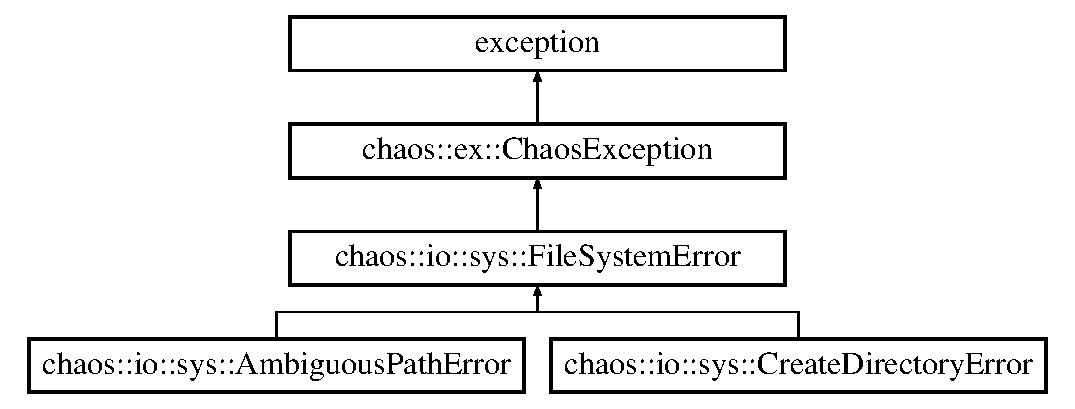
\includegraphics[height=4.000000cm]{classchaos_1_1io_1_1sys_1_1_file_system_error}
\end{center}
\end{figure}
\subsection*{Public Member Functions}
\begin{DoxyCompactItemize}
\item 
\hypertarget{classchaos_1_1io_1_1sys_1_1_file_system_error_a9da12ab81ffc6b146e6ac4bd60536bd2}{}{\bfseries File\+System\+Error} (const \hyperlink{classchaos_1_1uni_1_1_u_t_f8_string}{chaos\+::uni\+::\+U\+T\+F8\+String} \&message)\label{classchaos_1_1io_1_1sys_1_1_file_system_error_a9da12ab81ffc6b146e6ac4bd60536bd2}

\end{DoxyCompactItemize}
\subsection*{Additional Inherited Members}


\subsection{Detailed Description}
A generic error relating to the file system. 

All other file system exceptions inherit from this exception. 

The documentation for this class was generated from the following file\+:\begin{DoxyCompactItemize}
\item 
D\+:/\+Dropbox/\+Development/\+Chaos\+Core/\+Chaos\+Core/src/cxx/chaoscore/io/sys/\hyperlink{_file_system_exceptions_8hpp}{File\+System\+Exceptions.\+hpp}\end{DoxyCompactItemize}

\hypertarget{classchaos_1_1io_1_1sys_1_1_file_writer}{\section{chaos\-:\-:io\-:\-:sys\-:\-:File\-Writer Class Reference}
\label{classchaos_1_1io_1_1sys_1_1_file_writer}\index{chaos\-::io\-::sys\-::\-File\-Writer@{chaos\-::io\-::sys\-::\-File\-Writer}}
}


Object used to write to new or existing files on the file system.  




{\ttfamily \#include $<$File\-Writer.\-hpp$>$}

Inheritance diagram for chaos\-:\-:io\-:\-:sys\-:\-:File\-Writer\-:\begin{figure}[H]
\begin{center}
\leavevmode
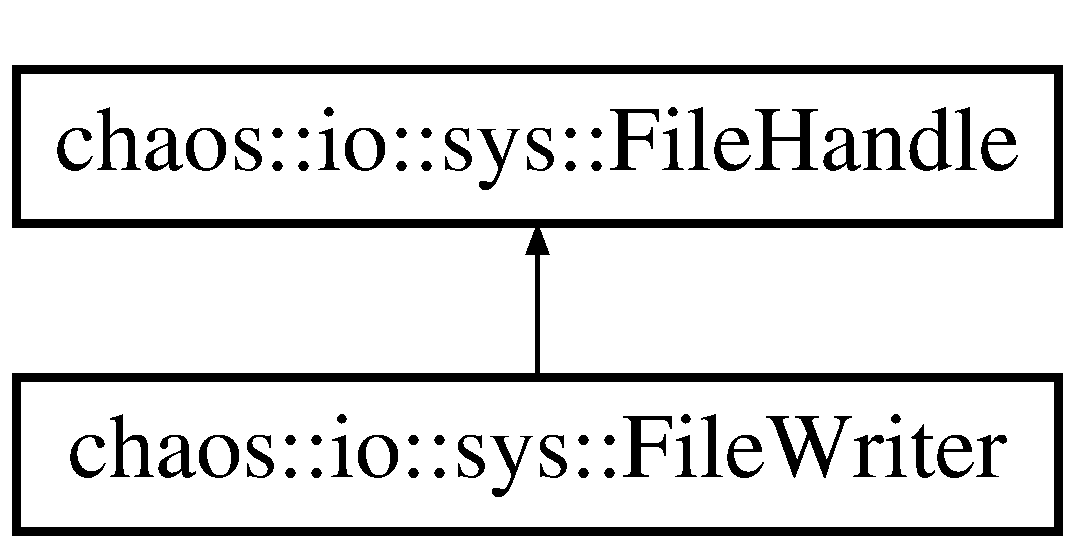
\includegraphics[height=2.000000cm]{classchaos_1_1io_1_1sys_1_1_file_writer}
\end{center}
\end{figure}
\subsection*{Public Types}
\begin{DoxyCompactItemize}
\item 
enum \hyperlink{classchaos_1_1io_1_1sys_1_1_file_writer_aafcaef6dd3171373d8dfadadcc3c1b0b}{Flag} \{ \hyperlink{classchaos_1_1io_1_1sys_1_1_file_writer_aafcaef6dd3171373d8dfadadcc3c1b0bab1c0f867f11da4ed8678148548fa9458}{F\-L\-A\-G\-\_\-\-N\-O\-N\-E}, 
\hyperlink{classchaos_1_1io_1_1sys_1_1_file_writer_aafcaef6dd3171373d8dfadadcc3c1b0baf46420535aaf1e5a6cf757485acaa2bc}{F\-L\-A\-G\-\_\-\-B\-I\-N\-A\-R\-Y}, 
\hyperlink{classchaos_1_1io_1_1sys_1_1_file_writer_aafcaef6dd3171373d8dfadadcc3c1b0ba2e28c6095d07cd49bee60edfcb9c4ec8}{F\-L\-A\-G\-\_\-\-A\-P\-P\-E\-N\-D}
 \}
\begin{DoxyCompactList}\small\item\em Flags that can be used to describe how the file handle should be opened. \end{DoxyCompactList}\end{DoxyCompactItemize}
\subsection*{Public Member Functions}
\begin{DoxyCompactItemize}
\item 
\hyperlink{classchaos_1_1io_1_1sys_1_1_file_writer_a84eee0f6699f145dd314201bbb60cab5}{File\-Writer} (\hyperlink{namespacechaos_a8641b3ae4551f0b35570d4f9f4ec22d9}{chaos\-::uint32} flags=\hyperlink{classchaos_1_1io_1_1sys_1_1_file_writer_aafcaef6dd3171373d8dfadadcc3c1b0bab1c0f867f11da4ed8678148548fa9458}{File\-Writer\-::\-F\-L\-A\-G\-\_\-\-N\-O\-N\-E})
\begin{DoxyCompactList}\small\item\em Default constructor. \end{DoxyCompactList}\item 
\hyperlink{classchaos_1_1io_1_1sys_1_1_file_writer_ade3f783fcaa44caf8ae1b3011e9847a1}{File\-Writer} (const \hyperlink{classchaos_1_1io_1_1sys_1_1_path}{chaos\-::io\-::sys\-::\-Path} \&path, \hyperlink{namespacechaos_a8641b3ae4551f0b35570d4f9f4ec22d9}{chaos\-::uint32} flags=\hyperlink{classchaos_1_1io_1_1sys_1_1_file_writer_aafcaef6dd3171373d8dfadadcc3c1b0bab1c0f867f11da4ed8678148548fa9458}{File\-Writer\-::\-F\-L\-A\-G\-\_\-\-N\-O\-N\-E})
\begin{DoxyCompactList}\small\item\em Open constructor. \end{DoxyCompactList}\item 
virtual void \hyperlink{classchaos_1_1io_1_1sys_1_1_file_writer_abddc915a52d4b589631d80bb24e013fe}{open} ()
\begin{DoxyCompactList}\small\item\em Opens the writer to the internal path. \end{DoxyCompactList}\end{DoxyCompactItemize}
\subsection*{Additional Inherited Members}


\subsection{Detailed Description}
Object used to write to new or existing files on the file system. 

T\-O\-D\-O\-: D\-O\-C, example use etc 

\subsection{Member Enumeration Documentation}
\hypertarget{classchaos_1_1io_1_1sys_1_1_file_writer_aafcaef6dd3171373d8dfadadcc3c1b0b}{\index{chaos\-::io\-::sys\-::\-File\-Writer@{chaos\-::io\-::sys\-::\-File\-Writer}!Flag@{Flag}}
\index{Flag@{Flag}!chaos::io::sys::FileWriter@{chaos\-::io\-::sys\-::\-File\-Writer}}
\subsubsection[{Flag}]{\setlength{\rightskip}{0pt plus 5cm}enum {\bf chaos\-::io\-::sys\-::\-File\-Writer\-::\-Flag}}}\label{classchaos_1_1io_1_1sys_1_1_file_writer_aafcaef6dd3171373d8dfadadcc3c1b0b}


Flags that can be used to describe how the file handle should be opened. 

These flags can be combined together using the logical or operator. \begin{Desc}
\item[Enumerator]\par
\begin{description}
\index{F\-L\-A\-G\-\_\-\-N\-O\-N\-E@{F\-L\-A\-G\-\_\-\-N\-O\-N\-E}!chaos\-::io\-::sys\-::\-File\-Writer@{chaos\-::io\-::sys\-::\-File\-Writer}}\index{chaos\-::io\-::sys\-::\-File\-Writer@{chaos\-::io\-::sys\-::\-File\-Writer}!F\-L\-A\-G\-\_\-\-N\-O\-N\-E@{F\-L\-A\-G\-\_\-\-N\-O\-N\-E}}\item[{\em 
\hypertarget{classchaos_1_1io_1_1sys_1_1_file_writer_aafcaef6dd3171373d8dfadadcc3c1b0bab1c0f867f11da4ed8678148548fa9458}{F\-L\-A\-G\-\_\-\-N\-O\-N\-E}\label{classchaos_1_1io_1_1sys_1_1_file_writer_aafcaef6dd3171373d8dfadadcc3c1b0bab1c0f867f11da4ed8678148548fa9458}
}]No flags specified. \index{F\-L\-A\-G\-\_\-\-B\-I\-N\-A\-R\-Y@{F\-L\-A\-G\-\_\-\-B\-I\-N\-A\-R\-Y}!chaos\-::io\-::sys\-::\-File\-Writer@{chaos\-::io\-::sys\-::\-File\-Writer}}\index{chaos\-::io\-::sys\-::\-File\-Writer@{chaos\-::io\-::sys\-::\-File\-Writer}!F\-L\-A\-G\-\_\-\-B\-I\-N\-A\-R\-Y@{F\-L\-A\-G\-\_\-\-B\-I\-N\-A\-R\-Y}}\item[{\em 
\hypertarget{classchaos_1_1io_1_1sys_1_1_file_writer_aafcaef6dd3171373d8dfadadcc3c1b0baf46420535aaf1e5a6cf757485acaa2bc}{F\-L\-A\-G\-\_\-\-B\-I\-N\-A\-R\-Y}\label{classchaos_1_1io_1_1sys_1_1_file_writer_aafcaef6dd3171373d8dfadadcc3c1b0baf46420535aaf1e5a6cf757485acaa2bc}
}]Operations are performed in binary mode rather than text mode. \index{F\-L\-A\-G\-\_\-\-A\-P\-P\-E\-N\-D@{F\-L\-A\-G\-\_\-\-A\-P\-P\-E\-N\-D}!chaos\-::io\-::sys\-::\-File\-Writer@{chaos\-::io\-::sys\-::\-File\-Writer}}\index{chaos\-::io\-::sys\-::\-File\-Writer@{chaos\-::io\-::sys\-::\-File\-Writer}!F\-L\-A\-G\-\_\-\-A\-P\-P\-E\-N\-D@{F\-L\-A\-G\-\_\-\-A\-P\-P\-E\-N\-D}}\item[{\em 
\hypertarget{classchaos_1_1io_1_1sys_1_1_file_writer_aafcaef6dd3171373d8dfadadcc3c1b0ba2e28c6095d07cd49bee60edfcb9c4ec8}{F\-L\-A\-G\-\_\-\-A\-P\-P\-E\-N\-D}\label{classchaos_1_1io_1_1sys_1_1_file_writer_aafcaef6dd3171373d8dfadadcc3c1b0ba2e28c6095d07cd49bee60edfcb9c4ec8}
}]If the file already exists new data will be written to the end of of the file. If this flag is not specified writing to existing file will cause the original contents to be discarded. \end{description}
\end{Desc}


\subsection{Constructor \& Destructor Documentation}
\hypertarget{classchaos_1_1io_1_1sys_1_1_file_writer_a84eee0f6699f145dd314201bbb60cab5}{\index{chaos\-::io\-::sys\-::\-File\-Writer@{chaos\-::io\-::sys\-::\-File\-Writer}!File\-Writer@{File\-Writer}}
\index{File\-Writer@{File\-Writer}!chaos::io::sys::FileWriter@{chaos\-::io\-::sys\-::\-File\-Writer}}
\subsubsection[{File\-Writer}]{\setlength{\rightskip}{0pt plus 5cm}chaos\-::io\-::sys\-::\-File\-Writer\-::\-File\-Writer (
\begin{DoxyParamCaption}
\item[{{\bf chaos\-::uint32}}]{flags = {\ttfamily {\bf File\-Writer\-::\-F\-L\-A\-G\-\_\-\-N\-O\-N\-E}}}
\end{DoxyParamCaption}
)}}\label{classchaos_1_1io_1_1sys_1_1_file_writer_a84eee0f6699f145dd314201bbb60cab5}


Default constructor. 

Creates a new unopened \hyperlink{classchaos_1_1io_1_1sys_1_1_file_writer}{File\-Writer} with no initial path set.


\begin{DoxyParams}{Parameters}
{\em flags} & Flags used to described how the \hyperlink{classchaos_1_1io_1_1sys_1_1_file_writer}{File\-Writer} should be opened. See \hyperlink{classchaos_1_1io_1_1sys_1_1_file_writer_aafcaef6dd3171373d8dfadadcc3c1b0b}{chaos\-::io\-::sys\-::\-File\-Writer\-::\-Flag} for more details. \\
\hline
\end{DoxyParams}
\hypertarget{classchaos_1_1io_1_1sys_1_1_file_writer_ade3f783fcaa44caf8ae1b3011e9847a1}{\index{chaos\-::io\-::sys\-::\-File\-Writer@{chaos\-::io\-::sys\-::\-File\-Writer}!File\-Writer@{File\-Writer}}
\index{File\-Writer@{File\-Writer}!chaos::io::sys::FileWriter@{chaos\-::io\-::sys\-::\-File\-Writer}}
\subsubsection[{File\-Writer}]{\setlength{\rightskip}{0pt plus 5cm}chaos\-::io\-::sys\-::\-File\-Writer\-::\-File\-Writer (
\begin{DoxyParamCaption}
\item[{const {\bf chaos\-::io\-::sys\-::\-Path} \&}]{path, }
\item[{{\bf chaos\-::uint32}}]{flags = {\ttfamily {\bf File\-Writer\-::\-F\-L\-A\-G\-\_\-\-N\-O\-N\-E}}}
\end{DoxyParamCaption}
)}}\label{classchaos_1_1io_1_1sys_1_1_file_writer_ade3f783fcaa44caf8ae1b3011e9847a1}


Open constructor. 

Creates a new \hyperlink{classchaos_1_1io_1_1sys_1_1_file_writer}{File\-Writer} and attempts to open it to the given path.


\begin{DoxyExceptions}{Exceptions}
{\em \hyperlink{classchaos_1_1io_1_1sys_1_1_invalid_path_error}{chaos\-::io\-::sys\-::\-Invalid\-Path\-Error}} & If the path cannot be opened\\
\hline
\end{DoxyExceptions}

\begin{DoxyParams}{Parameters}
{\em path} & \hyperlink{classchaos_1_1io_1_1sys_1_1_path}{Path} to open this \hyperlink{classchaos_1_1io_1_1sys_1_1_file_writer}{File\-Writer} to. \\
\hline
{\em flags} & Flags used to described how the \hyperlink{classchaos_1_1io_1_1sys_1_1_file_writer}{File\-Writer} should be opened.\\
\hline
\end{DoxyParams}
T\-O\-D\-O\-: doc flags 

\subsection{Member Function Documentation}
\hypertarget{classchaos_1_1io_1_1sys_1_1_file_writer_abddc915a52d4b589631d80bb24e013fe}{\index{chaos\-::io\-::sys\-::\-File\-Writer@{chaos\-::io\-::sys\-::\-File\-Writer}!open@{open}}
\index{open@{open}!chaos::io::sys::FileWriter@{chaos\-::io\-::sys\-::\-File\-Writer}}
\subsubsection[{open}]{\setlength{\rightskip}{0pt plus 5cm}virtual void chaos\-::io\-::sys\-::\-File\-Writer\-::open (
\begin{DoxyParamCaption}
{}
\end{DoxyParamCaption}
)\hspace{0.3cm}{\ttfamily [virtual]}}}\label{classchaos_1_1io_1_1sys_1_1_file_writer_abddc915a52d4b589631d80bb24e013fe}


Opens the writer to the internal path. 


\begin{DoxyExceptions}{Exceptions}
{\em \hyperlink{classchaos_1_1ex_1_1_state_error}{chaos\-::ex\-::\-State\-Error}} & If this file handle is already open.\\
\hline
{\em \hyperlink{classchaos_1_1io_1_1sys_1_1_invalid_path_error}{chaos\-::io\-::sys\-::\-Invalid\-Path\-Error}} & If the path cannot be opened \\
\hline
\end{DoxyExceptions}


Implements \hyperlink{classchaos_1_1io_1_1sys_1_1_file_handle_aaab721e850f11cd1f1bf3dba8e4ab2a1}{chaos\-::io\-::sys\-::\-File\-Handle}.



The documentation for this class was generated from the following file\-:\begin{DoxyCompactItemize}
\item 
/home/david/\-Dropbox/\-Development/\-Chaos\-Core/\-Chaos\-Core/src/cxx/chaoscore/io/sys/\hyperlink{_file_writer_8hpp}{File\-Writer.\-hpp}\end{DoxyCompactItemize}

\hypertarget{classchaos_1_1test_1_1_fixture}{\section{chaos\-:\-:test\-:\-:Fixture Class Reference}
\label{classchaos_1_1test_1_1_fixture}\index{chaos\-::test\-::\-Fixture@{chaos\-::test\-::\-Fixture}}
}


T\-O\-D\-O\-: D\-O\-C.  




{\ttfamily \#include $<$Chaos\-Test.\-hpp$>$}



\subsection{Detailed Description}
T\-O\-D\-O\-: D\-O\-C. 

T\-O\-D\-O\-: D\-O\-C 

The documentation for this class was generated from the following file\-:\begin{DoxyCompactItemize}
\item 
/home/david/\-Dropbox/\-Development/\-Chaos\-Core/\-Chaos\-Core/src/cxx/chaoscore/test/\hyperlink{_chaos_test_8hpp}{Chaos\-Test.\-hpp}\end{DoxyCompactItemize}

\hypertarget{classchaos_1_1ex_1_1_illegal_action_error}{}\section{chaos\+:\+:ex\+:\+:Illegal\+Action\+Error Class Reference}
\label{classchaos_1_1ex_1_1_illegal_action_error}\index{chaos\+::ex\+::\+Illegal\+Action\+Error@{chaos\+::ex\+::\+Illegal\+Action\+Error}}


Warns that an illegal action has been performed.  




{\ttfamily \#include $<$Base\+Exceptions.\+hpp$>$}

Inheritance diagram for chaos\+:\+:ex\+:\+:Illegal\+Action\+Error\+:\begin{figure}[H]
\begin{center}
\leavevmode
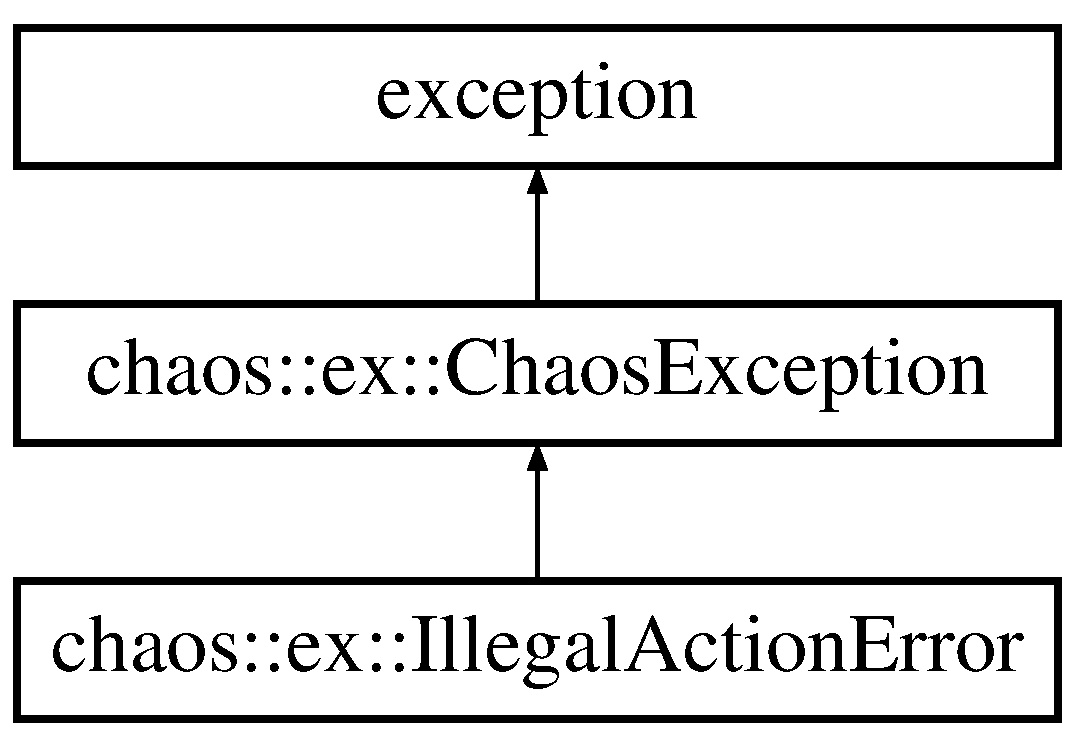
\includegraphics[height=3.000000cm]{classchaos_1_1ex_1_1_illegal_action_error}
\end{center}
\end{figure}
\subsection*{Public Member Functions}
\begin{DoxyCompactItemize}
\item 
\hypertarget{classchaos_1_1ex_1_1_illegal_action_error_a96fbdbcf8802979b3e4e10321edd4213}{}{\bfseries Illegal\+Action\+Error} (const \hyperlink{classchaos_1_1uni_1_1_u_t_f8_string}{chaos\+::uni\+::\+U\+T\+F8\+String} \&message)\label{classchaos_1_1ex_1_1_illegal_action_error_a96fbdbcf8802979b3e4e10321edd4213}

\end{DoxyCompactItemize}
\subsection*{Additional Inherited Members}


\subsection{Detailed Description}
Warns that an illegal action has been performed. 

The documentation for this class was generated from the following file\+:\begin{DoxyCompactItemize}
\item 
D\+:/\+Dropbox/\+Development/\+Chaos\+Core/\+Chaos\+Core/src/cxx/chaoscore/base/\hyperlink{_base_exceptions_8hpp}{Base\+Exceptions.\+hpp}\end{DoxyCompactItemize}

\hypertarget{classchaos_1_1ex_1_1_index_out_of_bounds_error}{\section{chaos\-:\-:ex\-:\-:Index\-Out\-Of\-Bounds\-Error Class Reference}
\label{classchaos_1_1ex_1_1_index_out_of_bounds_error}\index{chaos\-::ex\-::\-Index\-Out\-Of\-Bounds\-Error@{chaos\-::ex\-::\-Index\-Out\-Of\-Bounds\-Error}}
}


Warns that an index has been requested outside of the allowed bounds.  




{\ttfamily \#include $<$Base\-Exceptions.\-hpp$>$}

Inheritance diagram for chaos\-:\-:ex\-:\-:Index\-Out\-Of\-Bounds\-Error\-:\begin{figure}[H]
\begin{center}
\leavevmode
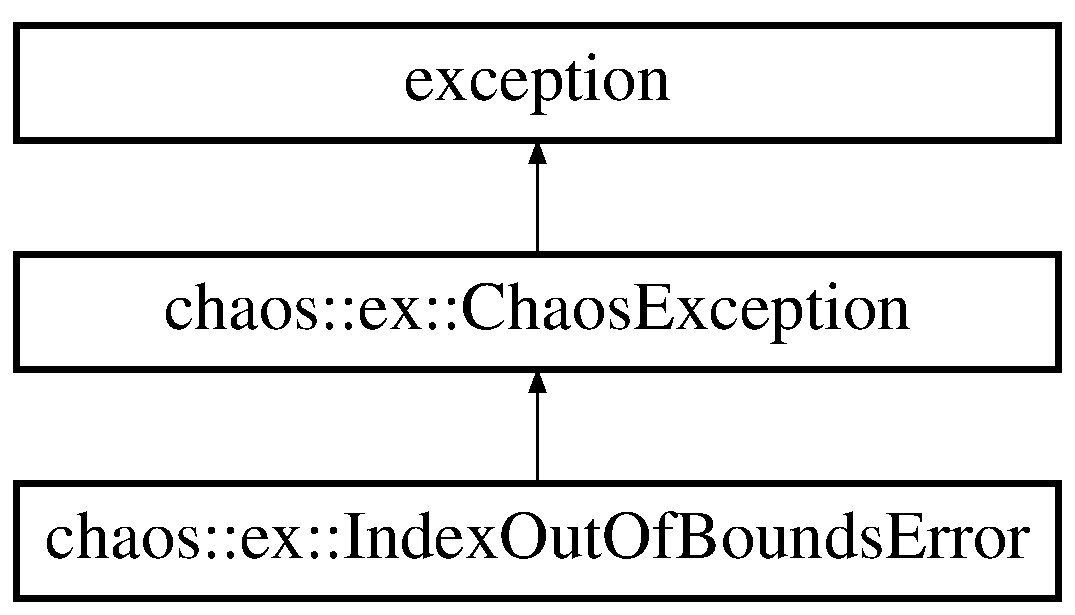
\includegraphics[height=3.000000cm]{classchaos_1_1ex_1_1_index_out_of_bounds_error}
\end{center}
\end{figure}
\subsection*{Public Member Functions}
\begin{DoxyCompactItemize}
\item 
\hypertarget{classchaos_1_1ex_1_1_index_out_of_bounds_error_a605674cdcd80159feffdc66bf4ae36f5}{{\bfseries Index\-Out\-Of\-Bounds\-Error} (const \hyperlink{classchaos_1_1str_1_1_u_t_f8_string}{chaos\-::str\-::\-U\-T\-F8\-String} \&message)}\label{classchaos_1_1ex_1_1_index_out_of_bounds_error_a605674cdcd80159feffdc66bf4ae36f5}

\end{DoxyCompactItemize}
\subsection*{Additional Inherited Members}


\subsection{Detailed Description}
Warns that an index has been requested outside of the allowed bounds. 

The documentation for this class was generated from the following file\-:\begin{DoxyCompactItemize}
\item 
/home/david/\-Dropbox/\-Development/\-Chaos\-Core/\-Chaos\-Core/src/cxx/chaoscore/base/\hyperlink{_base_exceptions_8hpp}{Base\-Exceptions.\-hpp}\end{DoxyCompactItemize}

\hypertarget{classchaos_1_1io_1_1sys_1_1_invalid_path_error}{}\section{chaos\+:\+:io\+:\+:sys\+:\+:Invalid\+Path\+Error Class Reference}
\label{classchaos_1_1io_1_1sys_1_1_invalid_path_error}\index{chaos\+::io\+::sys\+::\+Invalid\+Path\+Error@{chaos\+::io\+::sys\+::\+Invalid\+Path\+Error}}


Warns that given path cannot be accessed and/or modified because it does not exist permission is denied.  




{\ttfamily \#include $<$File\+System\+Exceptions.\+hpp$>$}

Inheritance diagram for chaos\+:\+:io\+:\+:sys\+:\+:Invalid\+Path\+Error\+:\begin{figure}[H]
\begin{center}
\leavevmode
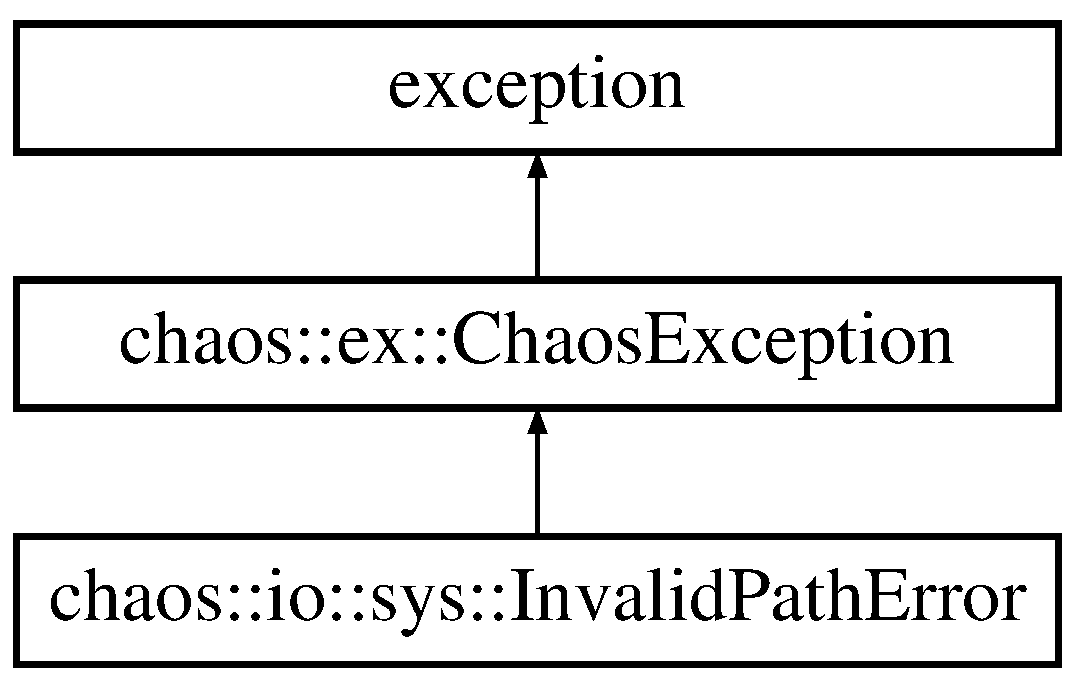
\includegraphics[height=3.000000cm]{classchaos_1_1io_1_1sys_1_1_invalid_path_error}
\end{center}
\end{figure}
\subsection*{Public Member Functions}
\begin{DoxyCompactItemize}
\item 
\hypertarget{classchaos_1_1io_1_1sys_1_1_invalid_path_error_a132ec813c227f40ffe9f3e3d64618a68}{}{\bfseries Invalid\+Path\+Error} (const \hyperlink{classchaos_1_1uni_1_1_u_t_f8_string}{chaos\+::uni\+::\+U\+T\+F8\+String} \&message)\label{classchaos_1_1io_1_1sys_1_1_invalid_path_error_a132ec813c227f40ffe9f3e3d64618a68}

\end{DoxyCompactItemize}
\subsection*{Additional Inherited Members}


\subsection{Detailed Description}
Warns that given path cannot be accessed and/or modified because it does not exist permission is denied. 

The documentation for this class was generated from the following file\+:\begin{DoxyCompactItemize}
\item 
D\+:/\+Dropbox/\+Development/\+Chaos\+Core/\+Chaos\+Core/src/cxx/chaoscore/io/sys/\hyperlink{_file_system_exceptions_8hpp}{File\+System\+Exceptions.\+hpp}\end{DoxyCompactItemize}

\hypertarget{classchaos_1_1ex_1_1_key_error}{\section{chaos\-:\-:ex\-:\-:Key\-Error Class Reference}
\label{classchaos_1_1ex_1_1_key_error}\index{chaos\-::ex\-::\-Key\-Error@{chaos\-::ex\-::\-Key\-Error}}
}


Warns that a map key has been requested that does not exist.  




{\ttfamily \#include $<$Base\-Exceptions.\-hpp$>$}

Inheritance diagram for chaos\-:\-:ex\-:\-:Key\-Error\-:\begin{figure}[H]
\begin{center}
\leavevmode
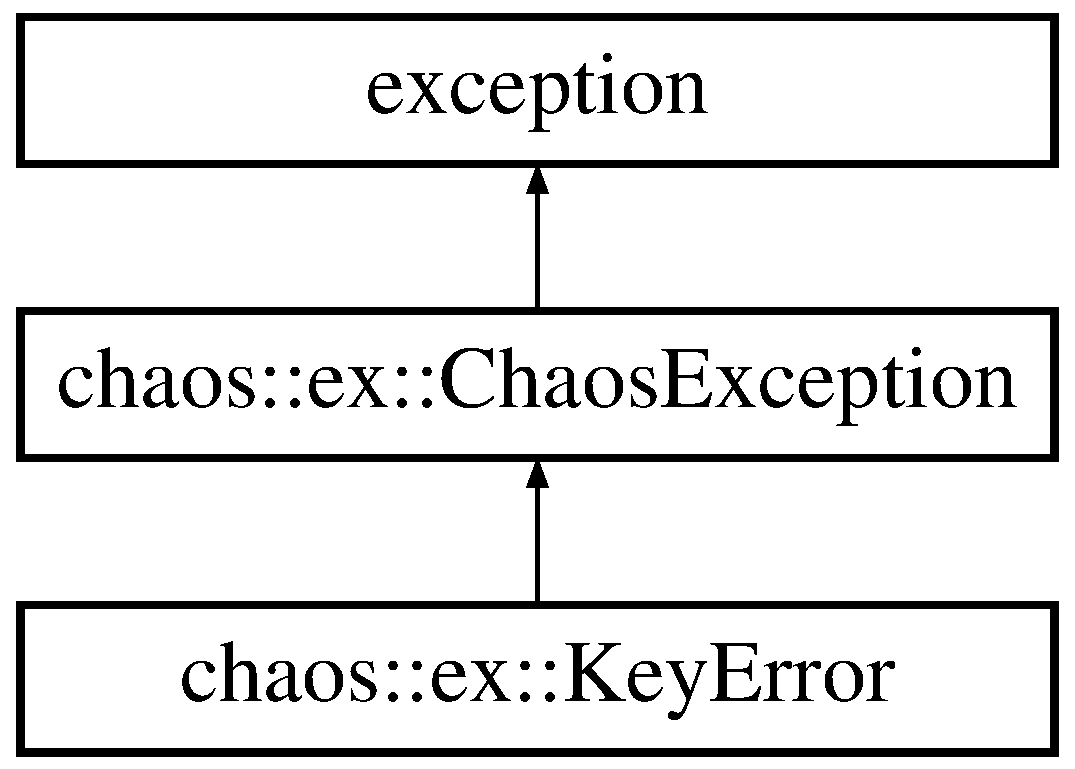
\includegraphics[height=3.000000cm]{classchaos_1_1ex_1_1_key_error}
\end{center}
\end{figure}
\subsection*{Public Member Functions}
\begin{DoxyCompactItemize}
\item 
\hypertarget{classchaos_1_1ex_1_1_key_error_ab784663047d04831ecb9150672a09b18}{{\bfseries Key\-Error} (const \hyperlink{classchaos_1_1uni_1_1_u_t_f8_string}{chaos\-::uni\-::\-U\-T\-F8\-String} \&message)}\label{classchaos_1_1ex_1_1_key_error_ab784663047d04831ecb9150672a09b18}

\end{DoxyCompactItemize}
\subsection*{Additional Inherited Members}


\subsection{Detailed Description}
Warns that a map key has been requested that does not exist. 

The documentation for this class was generated from the following file\-:\begin{DoxyCompactItemize}
\item 
/home/david/\-Dropbox/\-Development/\-Chaos\-Core/\-Chaos\-Core/src/cxx/chaoscore/base/\hyperlink{_base_exceptions_8hpp}{Base\-Exceptions.\-hpp}\end{DoxyCompactItemize}

\hypertarget{classchaos_1_1ex_1_1_not_implemented_error}{}\section{chaos\+:\+:ex\+:\+:Not\+Implemented\+Error Class Reference}
\label{classchaos_1_1ex_1_1_not_implemented_error}\index{chaos\+::ex\+::\+Not\+Implemented\+Error@{chaos\+::ex\+::\+Not\+Implemented\+Error}}


Warns that an operations has been performed that has not yet been implemented.  




{\ttfamily \#include $<$Base\+Exceptions.\+hpp$>$}

Inheritance diagram for chaos\+:\+:ex\+:\+:Not\+Implemented\+Error\+:\begin{figure}[H]
\begin{center}
\leavevmode
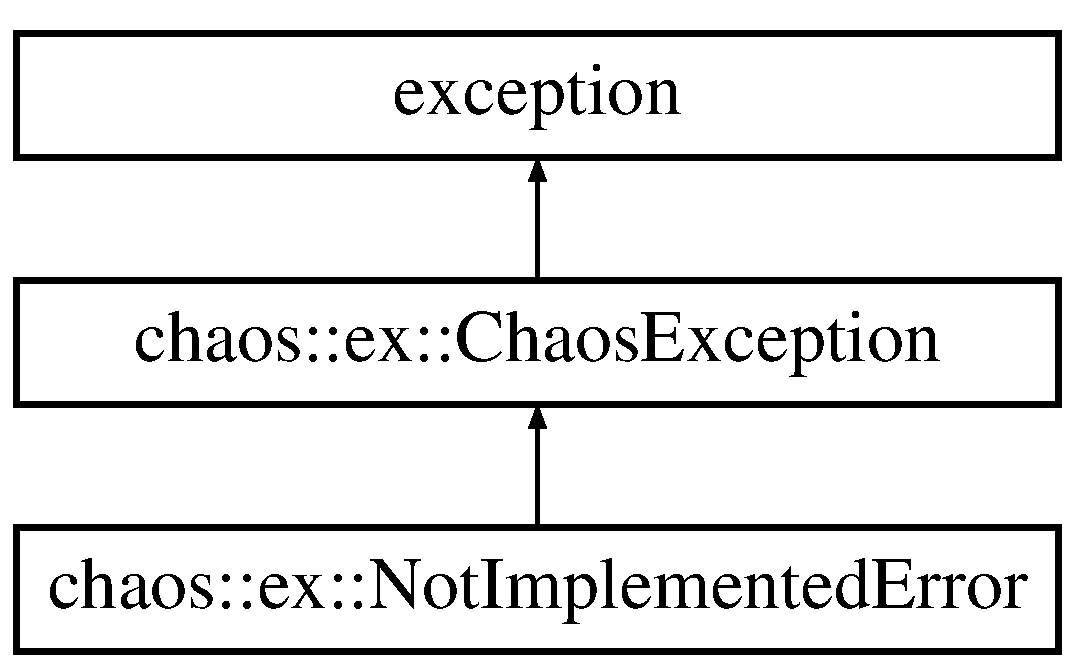
\includegraphics[height=3.000000cm]{classchaos_1_1ex_1_1_not_implemented_error}
\end{center}
\end{figure}
\subsection*{Public Member Functions}
\begin{DoxyCompactItemize}
\item 
\hypertarget{classchaos_1_1ex_1_1_not_implemented_error_a2e51452c959e229dfc4f46fad6c4c15f}{}{\bfseries Not\+Implemented\+Error} (const \hyperlink{classchaos_1_1uni_1_1_u_t_f8_string}{chaos\+::uni\+::\+U\+T\+F8\+String} \&message)\label{classchaos_1_1ex_1_1_not_implemented_error_a2e51452c959e229dfc4f46fad6c4c15f}

\end{DoxyCompactItemize}
\subsection*{Additional Inherited Members}


\subsection{Detailed Description}
Warns that an operations has been performed that has not yet been implemented. 

The documentation for this class was generated from the following file\+:\begin{DoxyCompactItemize}
\item 
D\+:/\+Dropbox/\+Development/\+Chaos\+Core/\+Chaos\+Core/src/cxx/chaoscore/base/\hyperlink{_base_exceptions_8hpp}{Base\+Exceptions.\+hpp}\end{DoxyCompactItemize}

\hypertarget{classchaos_1_1io_1_1sys_1_1_path}{\section{chaos\-:\-:io\-:\-:sys\-:\-:Path Class Reference}
\label{classchaos_1_1io_1_1sys_1_1_path}\index{chaos\-::io\-::sys\-::\-Path@{chaos\-::io\-::sys\-::\-Path}}
}


Represents a filesystem path.  




{\ttfamily \#include $<$Path.\-hpp$>$}

\subsection*{Public Member Functions}
\begin{DoxyCompactItemize}
\item 
\hyperlink{classchaos_1_1io_1_1sys_1_1_path_a4212b2acfcc365769080ea5e915568ee}{Path} ()
\begin{DoxyCompactList}\small\item\em Default constructor. \end{DoxyCompactList}\item 
\hyperlink{classchaos_1_1io_1_1sys_1_1_path_a3647583a07600e50e51d70f1dadabcf5}{Path} (const std\-::vector$<$ \hyperlink{classchaos_1_1uni_1_1_u_t_f8_string}{chaos\-::uni\-::\-U\-T\-F8\-String} $>$ \&components)
\begin{DoxyCompactList}\small\item\em Component constructor. \end{DoxyCompactList}\item 
\hyperlink{classchaos_1_1io_1_1sys_1_1_path_af77a957df51fe41a9c5df2d52ca05585}{Path} (const std\-::vector$<$ \hyperlink{classchaos_1_1uni_1_1_u_t_f8_string}{chaos\-::uni\-::\-U\-T\-F8\-String} $>$\-::const\-\_\-iterator \&begin, const std\-::vector$<$ \hyperlink{classchaos_1_1uni_1_1_u_t_f8_string}{chaos\-::uni\-::\-U\-T\-F8\-String} $>$\-::const\-\_\-iterator \&end)
\begin{DoxyCompactList}\small\item\em Iterator constructor. \end{DoxyCompactList}\item 
\hyperlink{classchaos_1_1io_1_1sys_1_1_path_a1a18b44624caafeceb66edc7b99dbad6}{Path} (const \hyperlink{classchaos_1_1uni_1_1_u_t_f8_string}{chaos\-::uni\-::\-U\-T\-F8\-String} \&string\-\_\-path)
\begin{DoxyCompactList}\small\item\em Attempts to create a \hyperlink{classchaos_1_1io_1_1sys_1_1_path}{Path} object from the given single string using the current operating system's path rules. \end{DoxyCompactList}\item 
\hyperlink{classchaos_1_1io_1_1sys_1_1_path_a40b3bf651b667adbd3eeb1ee55564211}{Path} (const \hyperlink{classchaos_1_1io_1_1sys_1_1_path}{Path} \&other)
\begin{DoxyCompactList}\small\item\em Copy constructor. \end{DoxyCompactList}\item 
const \hyperlink{classchaos_1_1io_1_1sys_1_1_path}{Path} \& \hyperlink{classchaos_1_1io_1_1sys_1_1_path_a45c70fc34ff619e890d5bc807dd70d8b}{operator=} (const \hyperlink{classchaos_1_1io_1_1sys_1_1_path}{Path} \&other)
\begin{DoxyCompactList}\small\item\em Assignment operator. \end{DoxyCompactList}\item 
bool \hyperlink{classchaos_1_1io_1_1sys_1_1_path_ac2e63307a0526625f4447f1d2a704e3b}{operator==} (const \hyperlink{classchaos_1_1io_1_1sys_1_1_path}{Path} \&other) const 
\begin{DoxyCompactList}\small\item\em Equality operator. \end{DoxyCompactList}\item 
bool \hyperlink{classchaos_1_1io_1_1sys_1_1_path_acd6dea0a797c0307179a5523239a299a}{operator!=} (const \hyperlink{classchaos_1_1io_1_1sys_1_1_path}{Path} \&other) const 
\begin{DoxyCompactList}\small\item\em Inequality operator. \end{DoxyCompactList}\item 
bool \hyperlink{classchaos_1_1io_1_1sys_1_1_path_a90858bbce348d5b36d0c31d771c601d8}{operator$<$} (const \hyperlink{classchaos_1_1io_1_1sys_1_1_path}{Path} \&other) const 
\begin{DoxyCompactList}\small\item\em Less than operator. \end{DoxyCompactList}\item 
\hyperlink{classchaos_1_1uni_1_1_u_t_f8_string}{chaos\-::uni\-::\-U\-T\-F8\-String} \& \hyperlink{classchaos_1_1io_1_1sys_1_1_path_ae7503e76ec85786225fc25b572deaeea}{operator\mbox{[}$\,$\mbox{]}} (size\-\_\-t index)
\begin{DoxyCompactList}\small\item\em Returns a reference to the component of this \hyperlink{classchaos_1_1io_1_1sys_1_1_path}{Path} at the given index. \end{DoxyCompactList}\item 
const \hyperlink{classchaos_1_1uni_1_1_u_t_f8_string}{chaos\-::uni\-::\-U\-T\-F8\-String} \& \hyperlink{classchaos_1_1io_1_1sys_1_1_path_aa3ee2fea4946e94c9bdb692bdffed522}{operator\mbox{[}$\,$\mbox{]}} (size\-\_\-t index) const 
\begin{DoxyCompactList}\small\item\em Returns a const reference to the component of this \hyperlink{classchaos_1_1io_1_1sys_1_1_path}{Path} at the given index. \end{DoxyCompactList}\item 
\hyperlink{classchaos_1_1io_1_1sys_1_1_path}{Path} \hyperlink{classchaos_1_1io_1_1sys_1_1_path_a5e769fd87717e15f0580e9aacbc0a418}{operator+} (const \hyperlink{classchaos_1_1io_1_1sys_1_1_path}{Path} \&other) const 
\begin{DoxyCompactList}\small\item\em Addition operator. \end{DoxyCompactList}\item 
const \hyperlink{classchaos_1_1io_1_1sys_1_1_path}{Path} \& \hyperlink{classchaos_1_1io_1_1sys_1_1_path_a92a616d9f16047d8933020bab54ed494}{operator+=} (const \hyperlink{classchaos_1_1io_1_1sys_1_1_path}{Path} \&other)
\begin{DoxyCompactList}\small\item\em Compound addition operator. \end{DoxyCompactList}\item 
\hyperlink{classchaos_1_1io_1_1sys_1_1_path}{Path} \& \hyperlink{classchaos_1_1io_1_1sys_1_1_path_a9b3f24e1f3bcb8e989c4b21d70d0a052}{operator$<$$<$} (const \hyperlink{classchaos_1_1uni_1_1_u_t_f8_string}{chaos\-::uni\-::\-U\-T\-F8\-String} \&component)
\begin{DoxyCompactList}\small\item\em Join operator. \end{DoxyCompactList}\item 
\hyperlink{classchaos_1_1io_1_1sys_1_1_path}{Path} \& \hyperlink{classchaos_1_1io_1_1sys_1_1_path_a8fcd75bd349c4c6d1286f6549e34de8c}{join} (const \hyperlink{classchaos_1_1uni_1_1_u_t_f8_string}{chaos\-::uni\-::\-U\-T\-F8\-String} \&component)
\begin{DoxyCompactList}\small\item\em Appends a new component to the end of this \hyperlink{classchaos_1_1io_1_1sys_1_1_path}{Path}. \end{DoxyCompactList}\item 
void \hyperlink{classchaos_1_1io_1_1sys_1_1_path_a7dc2fc570f8475ba5147bffb01de7025}{insert} (size\-\_\-t index, const \hyperlink{classchaos_1_1uni_1_1_u_t_f8_string}{chaos\-::uni\-::\-U\-T\-F8\-String} \&component)
\begin{DoxyCompactList}\small\item\em Inserts the component at the given index in this \hyperlink{classchaos_1_1io_1_1sys_1_1_path}{Path}. \end{DoxyCompactList}\item 
void \hyperlink{classchaos_1_1io_1_1sys_1_1_path_a7c4cd7e5d8e21a8c522f8a87f1e90f4c}{clear} ()
\begin{DoxyCompactList}\small\item\em Reverts this \hyperlink{classchaos_1_1io_1_1sys_1_1_path}{Path} to be an empty path. \end{DoxyCompactList}\item 
void \hyperlink{classchaos_1_1io_1_1sys_1_1_path_aefc69b11820209acca278104fb230832}{remove} (size\-\_\-t index)
\begin{DoxyCompactList}\small\item\em Removes the component from this \hyperlink{classchaos_1_1io_1_1sys_1_1_path}{Path} at the given index. \end{DoxyCompactList}\item 
const char $\ast$ \hyperlink{classchaos_1_1io_1_1sys_1_1_path_a9528370d2e3ab277a7e71a93469bbc45}{to\-\_\-native} () const 
\begin{DoxyCompactList}\small\item\em Returns a c string representation of this \hyperlink{classchaos_1_1io_1_1sys_1_1_path}{Path} for the current operating system. \end{DoxyCompactList}\item 
const char $\ast$ \hyperlink{classchaos_1_1io_1_1sys_1_1_path_acfc7975266821b34f97ed557b50bd4b5}{to\-\_\-unix} () const 
\begin{DoxyCompactList}\small\item\em Returns the \hyperlink{classchaos_1_1uni_1_1_u_t_f8_string}{chaos\-::uni\-::\-U\-T\-F8\-String} representation of this \hyperlink{classchaos_1_1io_1_1sys_1_1_path}{Path} for Unix based operating systems. \end{DoxyCompactList}\item 
const char $\ast$ \hyperlink{classchaos_1_1io_1_1sys_1_1_path_af36e2ca7305070fbcaa25ed6afa03201}{to\-\_\-windows} () const 
\begin{DoxyCompactList}\small\item\em Returns the \hyperlink{classchaos_1_1uni_1_1_u_t_f8_string}{chaos\-::uni\-::\-U\-T\-F8\-String} representation of this \hyperlink{classchaos_1_1io_1_1sys_1_1_path}{Path} for Windows based operating systems. \end{DoxyCompactList}\item 
\hyperlink{classchaos_1_1uni_1_1_u_t_f8_string}{chaos\-::uni\-::\-U\-T\-F8\-String} \hyperlink{classchaos_1_1io_1_1sys_1_1_path_a54f385bf11c8bf289adfb6ac3e8e9d46}{to\-\_\-native\-\_\-utf8} () const 
\begin{DoxyCompactList}\small\item\em Returns a \hyperlink{classchaos_1_1uni_1_1_u_t_f8_string}{chaos\-::uni\-::\-U\-T\-F8\-String} representation of this \hyperlink{classchaos_1_1io_1_1sys_1_1_path}{Path} for the current operating system. \end{DoxyCompactList}\item 
\hyperlink{classchaos_1_1uni_1_1_u_t_f8_string}{chaos\-::uni\-::\-U\-T\-F8\-String} \hyperlink{classchaos_1_1io_1_1sys_1_1_path_aa748ab64ab5d3b0efcd72a25947b5f35}{to\-\_\-unix\-\_\-utf8} () const 
\begin{DoxyCompactList}\small\item\em Returns the \hyperlink{classchaos_1_1uni_1_1_u_t_f8_string}{chaos\-::uni\-::\-U\-T\-F8\-String} representation of this \hyperlink{classchaos_1_1io_1_1sys_1_1_path}{Path} for Unix based operating systems. \end{DoxyCompactList}\item 
\hyperlink{classchaos_1_1uni_1_1_u_t_f8_string}{chaos\-::uni\-::\-U\-T\-F8\-String} \hyperlink{classchaos_1_1io_1_1sys_1_1_path_a02ef021f45851068ac79e9cd25c88298}{to\-\_\-windows\-\_\-utf8} () const 
\begin{DoxyCompactList}\small\item\em Returns the \hyperlink{classchaos_1_1uni_1_1_u_t_f8_string}{chaos\-::uni\-::\-U\-T\-F8\-String} representation of this \hyperlink{classchaos_1_1io_1_1sys_1_1_path}{Path} for Windows based operating systems. \end{DoxyCompactList}\item 
size\-\_\-t \hyperlink{classchaos_1_1io_1_1sys_1_1_path_a622fadb20bc01a0b58ef19eaf37fb44c}{get\-\_\-length} () const 
\begin{DoxyCompactList}\small\item\em Returns the number of components in this path. \end{DoxyCompactList}\item 
const std\-::vector\\*
$<$ \hyperlink{classchaos_1_1uni_1_1_u_t_f8_string}{chaos\-::uni\-::\-U\-T\-F8\-String} $>$ \& \hyperlink{classchaos_1_1io_1_1sys_1_1_path_ae20cae838af510b945e716d529e19bf4}{get\-\_\-components} () const 
\begin{DoxyCompactList}\small\item\em Returns the individual components which make up this path. \end{DoxyCompactList}\item 
\hyperlink{classchaos_1_1uni_1_1_u_t_f8_string}{chaos\-::uni\-::\-U\-T\-F8\-String} \hyperlink{classchaos_1_1io_1_1sys_1_1_path_ac7a2b7c374c1e4059b021b2c8751fb39}{get\-\_\-extension} () const 
\begin{DoxyCompactList}\small\item\em Returns the file extension of the leaf component of this \hyperlink{classchaos_1_1io_1_1sys_1_1_path}{Path}. \end{DoxyCompactList}\end{DoxyCompactItemize}


\subsection{Detailed Description}
Represents a filesystem path. 

The path this represents does not necessarily exists, nor does it have to be valid for the current operating system.

However this object is intended to provided platform independent methods for dealing with file system paths.

\begin{DoxyParagraph}{Example Usage}

\end{DoxyParagraph}
T\-O\-D\-O\-: 

\subsection{Constructor \& Destructor Documentation}
\hypertarget{classchaos_1_1io_1_1sys_1_1_path_a4212b2acfcc365769080ea5e915568ee}{\index{chaos\-::io\-::sys\-::\-Path@{chaos\-::io\-::sys\-::\-Path}!Path@{Path}}
\index{Path@{Path}!chaos::io::sys::Path@{chaos\-::io\-::sys\-::\-Path}}
\subsubsection[{Path}]{\setlength{\rightskip}{0pt plus 5cm}chaos\-::io\-::sys\-::\-Path\-::\-Path (
\begin{DoxyParamCaption}
{}
\end{DoxyParamCaption}
)}}\label{classchaos_1_1io_1_1sys_1_1_path_a4212b2acfcc365769080ea5e915568ee}


Default constructor. 

Creates a new empty \hyperlink{classchaos_1_1io_1_1sys_1_1_path}{Path}. \hypertarget{classchaos_1_1io_1_1sys_1_1_path_a3647583a07600e50e51d70f1dadabcf5}{\index{chaos\-::io\-::sys\-::\-Path@{chaos\-::io\-::sys\-::\-Path}!Path@{Path}}
\index{Path@{Path}!chaos::io::sys::Path@{chaos\-::io\-::sys\-::\-Path}}
\subsubsection[{Path}]{\setlength{\rightskip}{0pt plus 5cm}chaos\-::io\-::sys\-::\-Path\-::\-Path (
\begin{DoxyParamCaption}
\item[{const std\-::vector$<$ {\bf chaos\-::uni\-::\-U\-T\-F8\-String} $>$ \&}]{components}
\end{DoxyParamCaption}
)}}\label{classchaos_1_1io_1_1sys_1_1_path_a3647583a07600e50e51d70f1dadabcf5}


Component constructor. 

Creates a new \hyperlink{classchaos_1_1io_1_1sys_1_1_path}{Path} from the given std\-::vector of components.

For example the native Linux path\-:


\begin{DoxyCode}
path/to/file.txt
\end{DoxyCode}


Would be passed to this constructor like so\-:


\begin{DoxyCode}
std::vector< chaos::uni::UTF8String > components;
components.push\_back( \textcolor{stringliteral}{"path"} );
components.push\_back( \textcolor{stringliteral}{"to"} );
components.push\_back( \textcolor{stringliteral}{"file.txt"} );

chaos::io::file::Path p( components );
\end{DoxyCode}
 \hypertarget{classchaos_1_1io_1_1sys_1_1_path_af77a957df51fe41a9c5df2d52ca05585}{\index{chaos\-::io\-::sys\-::\-Path@{chaos\-::io\-::sys\-::\-Path}!Path@{Path}}
\index{Path@{Path}!chaos::io::sys::Path@{chaos\-::io\-::sys\-::\-Path}}
\subsubsection[{Path}]{\setlength{\rightskip}{0pt plus 5cm}chaos\-::io\-::sys\-::\-Path\-::\-Path (
\begin{DoxyParamCaption}
\item[{const std\-::vector$<$ {\bf chaos\-::uni\-::\-U\-T\-F8\-String} $>$\-::const\-\_\-iterator \&}]{begin, }
\item[{const std\-::vector$<$ {\bf chaos\-::uni\-::\-U\-T\-F8\-String} $>$\-::const\-\_\-iterator \&}]{end}
\end{DoxyParamCaption}
)}}\label{classchaos_1_1io_1_1sys_1_1_path_af77a957df51fe41a9c5df2d52ca05585}


Iterator constructor. 

Creates a new path from the components from the first iterator up to but not inclusive of the second iterator.

Example usage\-:


\begin{DoxyCode}
std::vector< chaos::uni::UTF8String > components;
components.push\_back( \textcolor{stringliteral}{"path"} );
components.push\_back( \textcolor{stringliteral}{"to"} );
components.push\_back( \textcolor{stringliteral}{"file.txt"} );

chaos::io::file::Path p( components.begin(), components.end() );
\end{DoxyCode}
 \hypertarget{classchaos_1_1io_1_1sys_1_1_path_a1a18b44624caafeceb66edc7b99dbad6}{\index{chaos\-::io\-::sys\-::\-Path@{chaos\-::io\-::sys\-::\-Path}!Path@{Path}}
\index{Path@{Path}!chaos::io::sys::Path@{chaos\-::io\-::sys\-::\-Path}}
\subsubsection[{Path}]{\setlength{\rightskip}{0pt plus 5cm}chaos\-::io\-::sys\-::\-Path\-::\-Path (
\begin{DoxyParamCaption}
\item[{const {\bf chaos\-::uni\-::\-U\-T\-F8\-String} \&}]{string\-\_\-path}
\end{DoxyParamCaption}
)}}\label{classchaos_1_1io_1_1sys_1_1_path_a1a18b44624caafeceb66edc7b99dbad6}


Attempts to create a \hyperlink{classchaos_1_1io_1_1sys_1_1_path}{Path} object from the given single string using the current operating system's path rules. 

\begin{DoxyNote}{Note}
This constructor method should be avoided where possible. Instead constructing paths using the $<$$<$ operator or \hyperlink{classchaos_1_1io_1_1sys_1_1_path_a8fcd75bd349c4c6d1286f6549e34de8c}{join()} function is recommended.
\end{DoxyNote}
On Unix systems this will split the given string into components using the \char`\"{}/\char`\"{} symbol. Likewise on Windows systems the \char`\"{}\textbackslash{}\char`\"{} symbol will be used. \hypertarget{classchaos_1_1io_1_1sys_1_1_path_a40b3bf651b667adbd3eeb1ee55564211}{\index{chaos\-::io\-::sys\-::\-Path@{chaos\-::io\-::sys\-::\-Path}!Path@{Path}}
\index{Path@{Path}!chaos::io::sys::Path@{chaos\-::io\-::sys\-::\-Path}}
\subsubsection[{Path}]{\setlength{\rightskip}{0pt plus 5cm}chaos\-::io\-::sys\-::\-Path\-::\-Path (
\begin{DoxyParamCaption}
\item[{const {\bf Path} \&}]{other}
\end{DoxyParamCaption}
)}}\label{classchaos_1_1io_1_1sys_1_1_path_a40b3bf651b667adbd3eeb1ee55564211}


Copy constructor. 

Creates a new \hyperlink{classchaos_1_1io_1_1sys_1_1_path}{Path} by copying the contents of the provided \hyperlink{classchaos_1_1io_1_1sys_1_1_path}{Path}. 

\subsection{Member Function Documentation}
\hypertarget{classchaos_1_1io_1_1sys_1_1_path_a45c70fc34ff619e890d5bc807dd70d8b}{\index{chaos\-::io\-::sys\-::\-Path@{chaos\-::io\-::sys\-::\-Path}!operator=@{operator=}}
\index{operator=@{operator=}!chaos::io::sys::Path@{chaos\-::io\-::sys\-::\-Path}}
\subsubsection[{operator=}]{\setlength{\rightskip}{0pt plus 5cm}const {\bf Path}\& chaos\-::io\-::sys\-::\-Path\-::operator= (
\begin{DoxyParamCaption}
\item[{const {\bf Path} \&}]{other}
\end{DoxyParamCaption}
)}}\label{classchaos_1_1io_1_1sys_1_1_path_a45c70fc34ff619e890d5bc807dd70d8b}


Assignment operator. 

Assigns the internal data of this \hyperlink{classchaos_1_1io_1_1sys_1_1_path}{Path} to be a copy of the data from the given \hyperlink{classchaos_1_1io_1_1sys_1_1_path}{Path}.


\begin{DoxyParams}{Parameters}
{\em other} & \hyperlink{classchaos_1_1io_1_1sys_1_1_path}{Path} to copy from. \\
\hline
\end{DoxyParams}
\begin{DoxyReturn}{Returns}
Reference to this \hyperlink{classchaos_1_1io_1_1sys_1_1_path}{Path} after the assignment has taken place. 
\end{DoxyReturn}
\hypertarget{classchaos_1_1io_1_1sys_1_1_path_ac2e63307a0526625f4447f1d2a704e3b}{\index{chaos\-::io\-::sys\-::\-Path@{chaos\-::io\-::sys\-::\-Path}!operator==@{operator==}}
\index{operator==@{operator==}!chaos::io::sys::Path@{chaos\-::io\-::sys\-::\-Path}}
\subsubsection[{operator==}]{\setlength{\rightskip}{0pt plus 5cm}bool chaos\-::io\-::sys\-::\-Path\-::operator== (
\begin{DoxyParamCaption}
\item[{const {\bf Path} \&}]{other}
\end{DoxyParamCaption}
) const}}\label{classchaos_1_1io_1_1sys_1_1_path_ac2e63307a0526625f4447f1d2a704e3b}


Equality operator. 

Compares whether this \hyperlink{classchaos_1_1io_1_1sys_1_1_path}{Path} and the other given \hyperlink{classchaos_1_1io_1_1sys_1_1_path}{Path} are considered equal.


\begin{DoxyParams}{Parameters}
{\em other} & \hyperlink{classchaos_1_1io_1_1sys_1_1_path}{Path} to compare this against. \\
\hline
\end{DoxyParams}
\begin{DoxyReturn}{Returns}
Whether the paths are equal. 
\end{DoxyReturn}
\hypertarget{classchaos_1_1io_1_1sys_1_1_path_acd6dea0a797c0307179a5523239a299a}{\index{chaos\-::io\-::sys\-::\-Path@{chaos\-::io\-::sys\-::\-Path}!operator!=@{operator!=}}
\index{operator!=@{operator!=}!chaos::io::sys::Path@{chaos\-::io\-::sys\-::\-Path}}
\subsubsection[{operator!=}]{\setlength{\rightskip}{0pt plus 5cm}bool chaos\-::io\-::sys\-::\-Path\-::operator!= (
\begin{DoxyParamCaption}
\item[{const {\bf Path} \&}]{other}
\end{DoxyParamCaption}
) const}}\label{classchaos_1_1io_1_1sys_1_1_path_acd6dea0a797c0307179a5523239a299a}


Inequality operator. 

Compares whether this \hyperlink{classchaos_1_1io_1_1sys_1_1_path}{Path} and the other given \hyperlink{classchaos_1_1io_1_1sys_1_1_path}{Path} are considered not equal.


\begin{DoxyParams}{Parameters}
{\em other} & \hyperlink{classchaos_1_1io_1_1sys_1_1_path}{Path} to compare this against. \\
\hline
\end{DoxyParams}
\begin{DoxyReturn}{Returns}
Whether the paths are equal. 
\end{DoxyReturn}
\hypertarget{classchaos_1_1io_1_1sys_1_1_path_a90858bbce348d5b36d0c31d771c601d8}{\index{chaos\-::io\-::sys\-::\-Path@{chaos\-::io\-::sys\-::\-Path}!operator$<$@{operator$<$}}
\index{operator$<$@{operator$<$}!chaos::io::sys::Path@{chaos\-::io\-::sys\-::\-Path}}
\subsubsection[{operator$<$}]{\setlength{\rightskip}{0pt plus 5cm}bool chaos\-::io\-::sys\-::\-Path\-::operator$<$ (
\begin{DoxyParamCaption}
\item[{const {\bf Path} \&}]{other}
\end{DoxyParamCaption}
) const}}\label{classchaos_1_1io_1_1sys_1_1_path_a90858bbce348d5b36d0c31d771c601d8}


Less than operator. 

Compares whether this \hyperlink{classchaos_1_1io_1_1sys_1_1_path}{Path} is considered less than the other given \hyperlink{classchaos_1_1io_1_1sys_1_1_path}{Path}.

\begin{DoxyNote}{Note}
This operator is primarily supplied so \hyperlink{classchaos_1_1io_1_1sys_1_1_path}{Path} objects can be stored in a std\-::map.
\end{DoxyNote}
Less than is defined by the number of components in a \hyperlink{classchaos_1_1io_1_1sys_1_1_path}{Path}, and if two paths have the same number of components then this resorts to a U\-T\-F8\-String less than comparison on each component until a mismatch is found.


\begin{DoxyParams}{Parameters}
{\em other} & \hyperlink{classchaos_1_1io_1_1sys_1_1_path}{Path} to compare this against. \\
\hline
\end{DoxyParams}
\begin{DoxyReturn}{Returns}
Whether this \hyperlink{classchaos_1_1io_1_1sys_1_1_path}{Path} is less than the other. 
\end{DoxyReturn}
\hypertarget{classchaos_1_1io_1_1sys_1_1_path_ae7503e76ec85786225fc25b572deaeea}{\index{chaos\-::io\-::sys\-::\-Path@{chaos\-::io\-::sys\-::\-Path}!operator\mbox{[}$\,$\mbox{]}@{operator[]}}
\index{operator\mbox{[}$\,$\mbox{]}@{operator[]}!chaos::io::sys::Path@{chaos\-::io\-::sys\-::\-Path}}
\subsubsection[{operator[]}]{\setlength{\rightskip}{0pt plus 5cm}{\bf chaos\-::uni\-::\-U\-T\-F8\-String}\& chaos\-::io\-::sys\-::\-Path\-::operator\mbox{[}$\,$\mbox{]} (
\begin{DoxyParamCaption}
\item[{size\-\_\-t}]{index}
\end{DoxyParamCaption}
)}}\label{classchaos_1_1io_1_1sys_1_1_path_ae7503e76ec85786225fc25b572deaeea}


Returns a reference to the component of this \hyperlink{classchaos_1_1io_1_1sys_1_1_path}{Path} at the given index. 


\begin{DoxyExceptions}{Exceptions}
{\em \hyperlink{classchaos_1_1ex_1_1_index_out_of_bounds_error}{chaos\-::ex\-::\-Index\-Out\-Of\-Bounds\-Error}} & If the provided index is out of bounds of the number of components in this \hyperlink{classchaos_1_1io_1_1sys_1_1_path}{Path}. \\
\hline
\end{DoxyExceptions}
\hypertarget{classchaos_1_1io_1_1sys_1_1_path_aa3ee2fea4946e94c9bdb692bdffed522}{\index{chaos\-::io\-::sys\-::\-Path@{chaos\-::io\-::sys\-::\-Path}!operator\mbox{[}$\,$\mbox{]}@{operator[]}}
\index{operator\mbox{[}$\,$\mbox{]}@{operator[]}!chaos::io::sys::Path@{chaos\-::io\-::sys\-::\-Path}}
\subsubsection[{operator[]}]{\setlength{\rightskip}{0pt plus 5cm}const {\bf chaos\-::uni\-::\-U\-T\-F8\-String}\& chaos\-::io\-::sys\-::\-Path\-::operator\mbox{[}$\,$\mbox{]} (
\begin{DoxyParamCaption}
\item[{size\-\_\-t}]{index}
\end{DoxyParamCaption}
) const}}\label{classchaos_1_1io_1_1sys_1_1_path_aa3ee2fea4946e94c9bdb692bdffed522}


Returns a const reference to the component of this \hyperlink{classchaos_1_1io_1_1sys_1_1_path}{Path} at the given index. 


\begin{DoxyExceptions}{Exceptions}
{\em \hyperlink{classchaos_1_1ex_1_1_index_out_of_bounds_error}{chaos\-::ex\-::\-Index\-Out\-Of\-Bounds\-Error}} & If the provided index is out of bounds of the number of components in this \hyperlink{classchaos_1_1io_1_1sys_1_1_path}{Path}. \\
\hline
\end{DoxyExceptions}
\hypertarget{classchaos_1_1io_1_1sys_1_1_path_a5e769fd87717e15f0580e9aacbc0a418}{\index{chaos\-::io\-::sys\-::\-Path@{chaos\-::io\-::sys\-::\-Path}!operator+@{operator+}}
\index{operator+@{operator+}!chaos::io::sys::Path@{chaos\-::io\-::sys\-::\-Path}}
\subsubsection[{operator+}]{\setlength{\rightskip}{0pt plus 5cm}{\bf Path} chaos\-::io\-::sys\-::\-Path\-::operator+ (
\begin{DoxyParamCaption}
\item[{const {\bf Path} \&}]{other}
\end{DoxyParamCaption}
) const}}\label{classchaos_1_1io_1_1sys_1_1_path_a5e769fd87717e15f0580e9aacbc0a418}


Addition operator. 

Creates a new \hyperlink{classchaos_1_1io_1_1sys_1_1_path}{Path} by extending the components of this \hyperlink{classchaos_1_1io_1_1sys_1_1_path}{Path} with the components of the other given \hyperlink{classchaos_1_1io_1_1sys_1_1_path}{Path}.

Example usage\-:


\begin{DoxyCode}
chaos::io::file::Path p1;
p1 << \textcolor{stringliteral}{"two"} << \textcolor{stringliteral}{"part"};

chaos::io::file::Path p2;
p2 << \textcolor{stringliteral}{"path"} << \textcolor{stringliteral}{"to"} << \textcolor{stringliteral}{"file.txt"};

chaos::io::file::Path p3 = p1 + p2;
\textcolor{comment}{// p3 contains [ "two", "part", "path", "to", "file.txt" ]}
\end{DoxyCode}
 \hypertarget{classchaos_1_1io_1_1sys_1_1_path_a92a616d9f16047d8933020bab54ed494}{\index{chaos\-::io\-::sys\-::\-Path@{chaos\-::io\-::sys\-::\-Path}!operator+=@{operator+=}}
\index{operator+=@{operator+=}!chaos::io::sys::Path@{chaos\-::io\-::sys\-::\-Path}}
\subsubsection[{operator+=}]{\setlength{\rightskip}{0pt plus 5cm}const {\bf Path}\& chaos\-::io\-::sys\-::\-Path\-::operator+= (
\begin{DoxyParamCaption}
\item[{const {\bf Path} \&}]{other}
\end{DoxyParamCaption}
)}}\label{classchaos_1_1io_1_1sys_1_1_path_a92a616d9f16047d8933020bab54ed494}


Compound addition operator. 

Extends this \hyperlink{classchaos_1_1io_1_1sys_1_1_path}{Path} with the components of the other given \hyperlink{classchaos_1_1io_1_1sys_1_1_path}{Path}.

Example usage\-:


\begin{DoxyCode}
chaos::io::file::Path p1;
p1 << \textcolor{stringliteral}{"two"} << \textcolor{stringliteral}{"part"};

chaos::io::file::Path p2;
p2 << \textcolor{stringliteral}{"path"} << \textcolor{stringliteral}{"to"} << \textcolor{stringliteral}{"file.txt"};

p1 += p2;
\textcolor{comment}{// p1 contains [ "two", "part", "path", "to", "file.txt" ]}
\end{DoxyCode}
 \hypertarget{classchaos_1_1io_1_1sys_1_1_path_a9b3f24e1f3bcb8e989c4b21d70d0a052}{\index{chaos\-::io\-::sys\-::\-Path@{chaos\-::io\-::sys\-::\-Path}!operator$<$$<$@{operator$<$$<$}}
\index{operator$<$$<$@{operator$<$$<$}!chaos::io::sys::Path@{chaos\-::io\-::sys\-::\-Path}}
\subsubsection[{operator$<$$<$}]{\setlength{\rightskip}{0pt plus 5cm}{\bf Path}\& chaos\-::io\-::sys\-::\-Path\-::operator$<$$<$ (
\begin{DoxyParamCaption}
\item[{const {\bf chaos\-::uni\-::\-U\-T\-F8\-String} \&}]{component}
\end{DoxyParamCaption}
)}}\label{classchaos_1_1io_1_1sys_1_1_path_a9b3f24e1f3bcb8e989c4b21d70d0a052}


Join operator. 

Appends a new component to end of this path. This is the same as using the \hyperlink{classchaos_1_1io_1_1sys_1_1_path_a8fcd75bd349c4c6d1286f6549e34de8c}{join()} function.

Example usage\-:


\begin{DoxyCode}
chaos::io::file::Path p;
p << \textcolor{stringliteral}{"path"} << \textcolor{stringliteral}{"to"} << \textcolor{stringliteral}{"file.txt"};
\textcolor{comment}{// p now contains [ "path", "to", "file" ]}
\end{DoxyCode}



\begin{DoxyParams}{Parameters}
{\em component} & String to be appended to the end of this \hyperlink{classchaos_1_1io_1_1sys_1_1_path}{Path} as a component. \\
\hline
\end{DoxyParams}
\begin{DoxyReturn}{Returns}
Reference to this \hyperlink{classchaos_1_1io_1_1sys_1_1_path}{Path} after the join has taken place. 
\end{DoxyReturn}
\hypertarget{classchaos_1_1io_1_1sys_1_1_path_a8fcd75bd349c4c6d1286f6549e34de8c}{\index{chaos\-::io\-::sys\-::\-Path@{chaos\-::io\-::sys\-::\-Path}!join@{join}}
\index{join@{join}!chaos::io::sys::Path@{chaos\-::io\-::sys\-::\-Path}}
\subsubsection[{join}]{\setlength{\rightskip}{0pt plus 5cm}{\bf Path}\& chaos\-::io\-::sys\-::\-Path\-::join (
\begin{DoxyParamCaption}
\item[{const {\bf chaos\-::uni\-::\-U\-T\-F8\-String} \&}]{component}
\end{DoxyParamCaption}
)}}\label{classchaos_1_1io_1_1sys_1_1_path_a8fcd75bd349c4c6d1286f6549e34de8c}


Appends a new component to the end of this \hyperlink{classchaos_1_1io_1_1sys_1_1_path}{Path}. 

Since this returns a non-\/const reference to this \hyperlink{classchaos_1_1io_1_1sys_1_1_path}{Path}, these functions can be chained.

Example usage\-:


\begin{DoxyCode}
chaos::io::file::Path p;
p.join( \textcolor{stringliteral}{"path"} ).join( \textcolor{stringliteral}{"to"} ).join( \textcolor{stringliteral}{"file.txt"} );
\textcolor{comment}{// p now contains [ "path", "to", "file" ]}
\end{DoxyCode}



\begin{DoxyParams}{Parameters}
{\em component} & \hyperlink{classchaos_1_1uni_1_1_u_t_f8_string}{chaos\-::uni\-::\-U\-T\-F8\-String} to be appended to the end of this \hyperlink{classchaos_1_1io_1_1sys_1_1_path}{Path} as a component. \\
\hline
\end{DoxyParams}
\begin{DoxyReturn}{Returns}
Reference to this \hyperlink{classchaos_1_1io_1_1sys_1_1_path}{Path} after the join has taken place. 
\end{DoxyReturn}
\hypertarget{classchaos_1_1io_1_1sys_1_1_path_a7dc2fc570f8475ba5147bffb01de7025}{\index{chaos\-::io\-::sys\-::\-Path@{chaos\-::io\-::sys\-::\-Path}!insert@{insert}}
\index{insert@{insert}!chaos::io::sys::Path@{chaos\-::io\-::sys\-::\-Path}}
\subsubsection[{insert}]{\setlength{\rightskip}{0pt plus 5cm}void chaos\-::io\-::sys\-::\-Path\-::insert (
\begin{DoxyParamCaption}
\item[{size\-\_\-t}]{index, }
\item[{const {\bf chaos\-::uni\-::\-U\-T\-F8\-String} \&}]{component}
\end{DoxyParamCaption}
)}}\label{classchaos_1_1io_1_1sys_1_1_path_a7dc2fc570f8475ba5147bffb01de7025}


Inserts the component at the given index in this \hyperlink{classchaos_1_1io_1_1sys_1_1_path}{Path}. 

If the index is less than the length of the string, the component currently at the index and all following components will be shuffled along one position.

If the index is equal to the current number of components in this \hyperlink{classchaos_1_1io_1_1sys_1_1_path}{Path}, this function is the same as calling \hyperlink{classchaos_1_1io_1_1sys_1_1_path_a8fcd75bd349c4c6d1286f6549e34de8c}{join()}.

If the index is greater than the number of components in this \hyperlink{classchaos_1_1io_1_1sys_1_1_path}{Path}, an exception will be thrown.

Example usage\-:


\begin{DoxyCode}
chaos::io::file::Path p;
p << \textcolor{stringliteral}{"path"} << \textcolor{stringliteral}{"file.txt"};
p.insert( 1, \textcolor{stringliteral}{"to"} );
\textcolor{comment}{// p now contains [ "path", "to", "file.txt" ]}
\end{DoxyCode}



\begin{DoxyExceptions}{Exceptions}
{\em \hyperlink{classchaos_1_1ex_1_1_index_out_of_bounds_error}{chaos\-::ex\-::\-Index\-Out\-Of\-Bounds\-Error}} & If the provided index is greater than the number of components currently in this \hyperlink{classchaos_1_1io_1_1sys_1_1_path}{Path}.\\
\hline
\end{DoxyExceptions}

\begin{DoxyParams}{Parameters}
{\em index} & Position to insert the new component at. \\
\hline
{\em component} & \hyperlink{classchaos_1_1uni_1_1_u_t_f8_string}{chaos\-::uni\-::\-U\-T\-F8\-String} representing the new component to be inserted. \\
\hline
\end{DoxyParams}
\hypertarget{classchaos_1_1io_1_1sys_1_1_path_a7c4cd7e5d8e21a8c522f8a87f1e90f4c}{\index{chaos\-::io\-::sys\-::\-Path@{chaos\-::io\-::sys\-::\-Path}!clear@{clear}}
\index{clear@{clear}!chaos::io::sys::Path@{chaos\-::io\-::sys\-::\-Path}}
\subsubsection[{clear}]{\setlength{\rightskip}{0pt plus 5cm}void chaos\-::io\-::sys\-::\-Path\-::clear (
\begin{DoxyParamCaption}
{}
\end{DoxyParamCaption}
)}}\label{classchaos_1_1io_1_1sys_1_1_path_a7c4cd7e5d8e21a8c522f8a87f1e90f4c}


Reverts this \hyperlink{classchaos_1_1io_1_1sys_1_1_path}{Path} to be an empty path. 

Clears any current components this \hyperlink{classchaos_1_1io_1_1sys_1_1_path}{Path} has. \hypertarget{classchaos_1_1io_1_1sys_1_1_path_aefc69b11820209acca278104fb230832}{\index{chaos\-::io\-::sys\-::\-Path@{chaos\-::io\-::sys\-::\-Path}!remove@{remove}}
\index{remove@{remove}!chaos::io::sys::Path@{chaos\-::io\-::sys\-::\-Path}}
\subsubsection[{remove}]{\setlength{\rightskip}{0pt plus 5cm}void chaos\-::io\-::sys\-::\-Path\-::remove (
\begin{DoxyParamCaption}
\item[{size\-\_\-t}]{index}
\end{DoxyParamCaption}
)}}\label{classchaos_1_1io_1_1sys_1_1_path_aefc69b11820209acca278104fb230832}


Removes the component from this \hyperlink{classchaos_1_1io_1_1sys_1_1_path}{Path} at the given index. 


\begin{DoxyExceptions}{Exceptions}
{\em \hyperlink{classchaos_1_1ex_1_1_index_out_of_bounds_error}{chaos\-::ex\-::\-Index\-Out\-Of\-Bounds\-Error}} & If the provided index is out of bounds of the number of components in this \hyperlink{classchaos_1_1io_1_1sys_1_1_path}{Path}.\\
\hline
\end{DoxyExceptions}

\begin{DoxyParams}{Parameters}
{\em index} & The index of the component to remove from this path. \\
\hline
\end{DoxyParams}
\hypertarget{classchaos_1_1io_1_1sys_1_1_path_a9528370d2e3ab277a7e71a93469bbc45}{\index{chaos\-::io\-::sys\-::\-Path@{chaos\-::io\-::sys\-::\-Path}!to\-\_\-native@{to\-\_\-native}}
\index{to\-\_\-native@{to\-\_\-native}!chaos::io::sys::Path@{chaos\-::io\-::sys\-::\-Path}}
\subsubsection[{to\-\_\-native}]{\setlength{\rightskip}{0pt plus 5cm}const char$\ast$ chaos\-::io\-::sys\-::\-Path\-::to\-\_\-native (
\begin{DoxyParamCaption}
{}
\end{DoxyParamCaption}
) const}}\label{classchaos_1_1io_1_1sys_1_1_path_a9528370d2e3ab277a7e71a93469bbc45}


Returns a c string representation of this \hyperlink{classchaos_1_1io_1_1sys_1_1_path}{Path} for the current operating system. 

Example usage\-:


\begin{DoxyCode}
chaos::io::file::Path p;
p << \textcolor{stringliteral}{"path"} << \textcolor{stringliteral}{"to"} << \textcolor{stringliteral}{"file.txt"};
\textcolor{keyword}{const} \textcolor{keywordtype}{char}* s = p.to\_native();
\textcolor{comment}{// on Unix systems s will be "path/to/file.txt"}
\textcolor{comment}{// on Windows systems s will be "path\(\backslash\)to\(\backslash\)file.txt"}
\end{DoxyCode}


\begin{DoxyNote}{Note}
This operation returns a c style string to support platform dependent encodings. For example Windows requires non-\/ascii file paths to be U\-T\-F-\/16 encoded, therefore the returned c string will be utf-\/16 encoded. Likewise on Unix systems this string will be utf-\/8 encoded. To get \hyperlink{classchaos_1_1uni_1_1_u_t_f8_string}{chaos\-::uni\-::\-U\-T\-F8\-String} representations of this path see \hyperlink{classchaos_1_1io_1_1sys_1_1_path_a54f385bf11c8bf289adfb6ac3e8e9d46}{to\-\_\-native\-\_\-utf8()}, \hyperlink{classchaos_1_1io_1_1sys_1_1_path_aa748ab64ab5d3b0efcd72a25947b5f35}{to\-\_\-unix\-\_\-utf8()}, and \hyperlink{classchaos_1_1io_1_1sys_1_1_path_a02ef021f45851068ac79e9cd25c88298}{to\-\_\-windows\-\_\-utf8()}.
\end{DoxyNote}
\begin{DoxyWarning}{Warning}
The returned string is allocated by this object and will be only exist for the life time of this \hyperlink{classchaos_1_1io_1_1sys_1_1_path}{Path} object. 
\end{DoxyWarning}
\hypertarget{classchaos_1_1io_1_1sys_1_1_path_acfc7975266821b34f97ed557b50bd4b5}{\index{chaos\-::io\-::sys\-::\-Path@{chaos\-::io\-::sys\-::\-Path}!to\-\_\-unix@{to\-\_\-unix}}
\index{to\-\_\-unix@{to\-\_\-unix}!chaos::io::sys::Path@{chaos\-::io\-::sys\-::\-Path}}
\subsubsection[{to\-\_\-unix}]{\setlength{\rightskip}{0pt plus 5cm}const char$\ast$ chaos\-::io\-::sys\-::\-Path\-::to\-\_\-unix (
\begin{DoxyParamCaption}
{}
\end{DoxyParamCaption}
) const}}\label{classchaos_1_1io_1_1sys_1_1_path_acfc7975266821b34f97ed557b50bd4b5}


Returns the \hyperlink{classchaos_1_1uni_1_1_u_t_f8_string}{chaos\-::uni\-::\-U\-T\-F8\-String} representation of this \hyperlink{classchaos_1_1io_1_1sys_1_1_path}{Path} for Unix based operating systems. 

Example usage\-:


\begin{DoxyCode}
chaos::io::file::Path p;
p << \textcolor{stringliteral}{"path"} << \textcolor{stringliteral}{"to"} << \textcolor{stringliteral}{"file.txt"};
\textcolor{keyword}{const} \textcolor{keywordtype}{char}*  s = p.to\_unix();
\textcolor{comment}{// s is "path/to/file.txt"}
\end{DoxyCode}


\begin{DoxyNote}{Note}
This operation returns a c style string to support platform dependent encodings. For example Windows requires non-\/ascii file paths to be U\-T\-F-\/16 encoded, therefore the returned c string will be utf-\/16 encoded. Likewise on Unix systems this string will be utf-\/8 encoded. To get \hyperlink{classchaos_1_1uni_1_1_u_t_f8_string}{chaos\-::uni\-::\-U\-T\-F8\-String} representations of this path see \hyperlink{classchaos_1_1io_1_1sys_1_1_path_a54f385bf11c8bf289adfb6ac3e8e9d46}{to\-\_\-native\-\_\-utf8()}, \hyperlink{classchaos_1_1io_1_1sys_1_1_path_aa748ab64ab5d3b0efcd72a25947b5f35}{to\-\_\-unix\-\_\-utf8()}, and \hyperlink{classchaos_1_1io_1_1sys_1_1_path_a02ef021f45851068ac79e9cd25c88298}{to\-\_\-windows\-\_\-utf8()}.
\end{DoxyNote}
\begin{DoxyWarning}{Warning}
The returned string is allocated by this object and will be only exist for the life time of this \hyperlink{classchaos_1_1io_1_1sys_1_1_path}{Path} object. 
\end{DoxyWarning}
\hypertarget{classchaos_1_1io_1_1sys_1_1_path_af36e2ca7305070fbcaa25ed6afa03201}{\index{chaos\-::io\-::sys\-::\-Path@{chaos\-::io\-::sys\-::\-Path}!to\-\_\-windows@{to\-\_\-windows}}
\index{to\-\_\-windows@{to\-\_\-windows}!chaos::io::sys::Path@{chaos\-::io\-::sys\-::\-Path}}
\subsubsection[{to\-\_\-windows}]{\setlength{\rightskip}{0pt plus 5cm}const char$\ast$ chaos\-::io\-::sys\-::\-Path\-::to\-\_\-windows (
\begin{DoxyParamCaption}
{}
\end{DoxyParamCaption}
) const}}\label{classchaos_1_1io_1_1sys_1_1_path_af36e2ca7305070fbcaa25ed6afa03201}


Returns the \hyperlink{classchaos_1_1uni_1_1_u_t_f8_string}{chaos\-::uni\-::\-U\-T\-F8\-String} representation of this \hyperlink{classchaos_1_1io_1_1sys_1_1_path}{Path} for Windows based operating systems. 

Example usage\-:


\begin{DoxyCode}
chaos::io::file::Path p;
p << \textcolor{stringliteral}{"path"} << \textcolor{stringliteral}{"to"} << \textcolor{stringliteral}{"file.txt"};
\textcolor{keyword}{const} \textcolor{keywordtype}{char}*  s = p.to\_windows();
\textcolor{comment}{// s is "path\(\backslash\)to\(\backslash\)file.txt"}
\end{DoxyCode}


\begin{DoxyNote}{Note}
This operation returns a c style string to support platform dependent encodings. For example Windows requires non-\/ascii file paths to be U\-T\-F-\/16 encoded, therefore the returned c string will be utf-\/16 encoded. Likewise on Unix systems this string will be utf-\/8 encoded. To get \hyperlink{classchaos_1_1uni_1_1_u_t_f8_string}{chaos\-::uni\-::\-U\-T\-F8\-String} representations of this path see \hyperlink{classchaos_1_1io_1_1sys_1_1_path_a54f385bf11c8bf289adfb6ac3e8e9d46}{to\-\_\-native\-\_\-utf8()}, \hyperlink{classchaos_1_1io_1_1sys_1_1_path_aa748ab64ab5d3b0efcd72a25947b5f35}{to\-\_\-unix\-\_\-utf8()}, and \hyperlink{classchaos_1_1io_1_1sys_1_1_path_a02ef021f45851068ac79e9cd25c88298}{to\-\_\-windows\-\_\-utf8()}.
\end{DoxyNote}
\begin{DoxyWarning}{Warning}
The returned string is allocated by this object and will be only exist for the life time of this \hyperlink{classchaos_1_1io_1_1sys_1_1_path}{Path} object. 
\end{DoxyWarning}
\hypertarget{classchaos_1_1io_1_1sys_1_1_path_a54f385bf11c8bf289adfb6ac3e8e9d46}{\index{chaos\-::io\-::sys\-::\-Path@{chaos\-::io\-::sys\-::\-Path}!to\-\_\-native\-\_\-utf8@{to\-\_\-native\-\_\-utf8}}
\index{to\-\_\-native\-\_\-utf8@{to\-\_\-native\-\_\-utf8}!chaos::io::sys::Path@{chaos\-::io\-::sys\-::\-Path}}
\subsubsection[{to\-\_\-native\-\_\-utf8}]{\setlength{\rightskip}{0pt plus 5cm}{\bf chaos\-::uni\-::\-U\-T\-F8\-String} chaos\-::io\-::sys\-::\-Path\-::to\-\_\-native\-\_\-utf8 (
\begin{DoxyParamCaption}
{}
\end{DoxyParamCaption}
) const}}\label{classchaos_1_1io_1_1sys_1_1_path_a54f385bf11c8bf289adfb6ac3e8e9d46}


Returns a \hyperlink{classchaos_1_1uni_1_1_u_t_f8_string}{chaos\-::uni\-::\-U\-T\-F8\-String} representation of this \hyperlink{classchaos_1_1io_1_1sys_1_1_path}{Path} for the current operating system. 

Example usage\-:


\begin{DoxyCode}
chaos::io::file::Path p;
p << \textcolor{stringliteral}{"path"} << \textcolor{stringliteral}{"to"} << \textcolor{stringliteral}{"file.txt"};
\hyperlink{classchaos_1_1uni_1_1_u_t_f8_string}{chaos::uni::UTF8String} s = p.to\_native\_utf8();
\textcolor{comment}{// on Unix systems s will be "path/to/file.txt"}
\textcolor{comment}{// on Windows systems s will be "path\(\backslash\)to\(\backslash\)file.txt"}
\end{DoxyCode}


\begin{DoxyNote}{Note}
This operation returns a c style string to support platform dependent encodings. For example Windows requires non-\/ascii file paths to be U\-T\-F-\/16 encoded, therefore the returned c string will be utf-\/16 encoded. Likewise on Unix systems this string will be utf-\/8 encoded. To get \hyperlink{classchaos_1_1uni_1_1_u_t_f8_string}{chaos\-::uni\-::\-U\-T\-F8\-String} representations of this path see \hyperlink{classchaos_1_1io_1_1sys_1_1_path_a54f385bf11c8bf289adfb6ac3e8e9d46}{to\-\_\-native\-\_\-utf8()}, \hyperlink{classchaos_1_1io_1_1sys_1_1_path_aa748ab64ab5d3b0efcd72a25947b5f35}{to\-\_\-unix\-\_\-utf8()}, and \hyperlink{classchaos_1_1io_1_1sys_1_1_path_a02ef021f45851068ac79e9cd25c88298}{to\-\_\-windows\-\_\-utf8()}. 
\end{DoxyNote}
\hypertarget{classchaos_1_1io_1_1sys_1_1_path_aa748ab64ab5d3b0efcd72a25947b5f35}{\index{chaos\-::io\-::sys\-::\-Path@{chaos\-::io\-::sys\-::\-Path}!to\-\_\-unix\-\_\-utf8@{to\-\_\-unix\-\_\-utf8}}
\index{to\-\_\-unix\-\_\-utf8@{to\-\_\-unix\-\_\-utf8}!chaos::io::sys::Path@{chaos\-::io\-::sys\-::\-Path}}
\subsubsection[{to\-\_\-unix\-\_\-utf8}]{\setlength{\rightskip}{0pt plus 5cm}{\bf chaos\-::uni\-::\-U\-T\-F8\-String} chaos\-::io\-::sys\-::\-Path\-::to\-\_\-unix\-\_\-utf8 (
\begin{DoxyParamCaption}
{}
\end{DoxyParamCaption}
) const}}\label{classchaos_1_1io_1_1sys_1_1_path_aa748ab64ab5d3b0efcd72a25947b5f35}


Returns the \hyperlink{classchaos_1_1uni_1_1_u_t_f8_string}{chaos\-::uni\-::\-U\-T\-F8\-String} representation of this \hyperlink{classchaos_1_1io_1_1sys_1_1_path}{Path} for Unix based operating systems. 

Example usage\-:


\begin{DoxyCode}
chaos::io::file::Path p;
p << \textcolor{stringliteral}{"path"} << \textcolor{stringliteral}{"to"} << \textcolor{stringliteral}{"file.txt"};
\hyperlink{classchaos_1_1uni_1_1_u_t_f8_string}{chaos::uni::UTF8String} s = p.to\_unix\_utf8();
\textcolor{comment}{// s is "path/to/file.txt"}
\end{DoxyCode}
 \hypertarget{classchaos_1_1io_1_1sys_1_1_path_a02ef021f45851068ac79e9cd25c88298}{\index{chaos\-::io\-::sys\-::\-Path@{chaos\-::io\-::sys\-::\-Path}!to\-\_\-windows\-\_\-utf8@{to\-\_\-windows\-\_\-utf8}}
\index{to\-\_\-windows\-\_\-utf8@{to\-\_\-windows\-\_\-utf8}!chaos::io::sys::Path@{chaos\-::io\-::sys\-::\-Path}}
\subsubsection[{to\-\_\-windows\-\_\-utf8}]{\setlength{\rightskip}{0pt plus 5cm}{\bf chaos\-::uni\-::\-U\-T\-F8\-String} chaos\-::io\-::sys\-::\-Path\-::to\-\_\-windows\-\_\-utf8 (
\begin{DoxyParamCaption}
{}
\end{DoxyParamCaption}
) const}}\label{classchaos_1_1io_1_1sys_1_1_path_a02ef021f45851068ac79e9cd25c88298}


Returns the \hyperlink{classchaos_1_1uni_1_1_u_t_f8_string}{chaos\-::uni\-::\-U\-T\-F8\-String} representation of this \hyperlink{classchaos_1_1io_1_1sys_1_1_path}{Path} for Windows based operating systems. 

Example usage\-:


\begin{DoxyCode}
chaos::io::file::Path p;
p << \textcolor{stringliteral}{"path"} << \textcolor{stringliteral}{"to"} << \textcolor{stringliteral}{"file.txt"};
\hyperlink{classchaos_1_1uni_1_1_u_t_f8_string}{chaos::uni::UTF8String} s = p.to\_windows\_utf8();
\textcolor{comment}{// s is "path\(\backslash\)to\(\backslash\)file.txt"}
\end{DoxyCode}
 \hypertarget{classchaos_1_1io_1_1sys_1_1_path_a622fadb20bc01a0b58ef19eaf37fb44c}{\index{chaos\-::io\-::sys\-::\-Path@{chaos\-::io\-::sys\-::\-Path}!get\-\_\-length@{get\-\_\-length}}
\index{get\-\_\-length@{get\-\_\-length}!chaos::io::sys::Path@{chaos\-::io\-::sys\-::\-Path}}
\subsubsection[{get\-\_\-length}]{\setlength{\rightskip}{0pt plus 5cm}size\-\_\-t chaos\-::io\-::sys\-::\-Path\-::get\-\_\-length (
\begin{DoxyParamCaption}
{}
\end{DoxyParamCaption}
) const}}\label{classchaos_1_1io_1_1sys_1_1_path_a622fadb20bc01a0b58ef19eaf37fb44c}


Returns the number of components in this path. 

Example usage\-:


\begin{DoxyCode}
chaos::io::file::Path p;
p << \textcolor{stringliteral}{"path"} << \textcolor{stringliteral}{"to"} << \textcolor{stringliteral}{"file.txt"};
p.get\_length(); \textcolor{comment}{// returns: 3}
\end{DoxyCode}
 \hypertarget{classchaos_1_1io_1_1sys_1_1_path_ae20cae838af510b945e716d529e19bf4}{\index{chaos\-::io\-::sys\-::\-Path@{chaos\-::io\-::sys\-::\-Path}!get\-\_\-components@{get\-\_\-components}}
\index{get\-\_\-components@{get\-\_\-components}!chaos::io::sys::Path@{chaos\-::io\-::sys\-::\-Path}}
\subsubsection[{get\-\_\-components}]{\setlength{\rightskip}{0pt plus 5cm}const std\-::vector$<$ {\bf chaos\-::uni\-::\-U\-T\-F8\-String} $>$\& chaos\-::io\-::sys\-::\-Path\-::get\-\_\-components (
\begin{DoxyParamCaption}
{}
\end{DoxyParamCaption}
) const}}\label{classchaos_1_1io_1_1sys_1_1_path_ae20cae838af510b945e716d529e19bf4}


Returns the individual components which make up this path. 

For example the native Linux path\-:


\begin{DoxyCode}
path/to/file.txt
\end{DoxyCode}


Stored correctly in a \hyperlink{classchaos_1_1io_1_1sys_1_1_path}{Path} object\-:


\begin{DoxyCode}
chaos::io::file::Path path;
path << \textcolor{stringliteral}{"path"} << \textcolor{stringliteral}{"to"} << \textcolor{stringliteral}{"file.txt"};
\end{DoxyCode}


Would contain the components\-:


\begin{DoxyCode}
[ \textcolor{stringliteral}{"path"}, \textcolor{stringliteral}{"to"}, \textcolor{stringliteral}{"file.txt"} ]
\end{DoxyCode}
 \hypertarget{classchaos_1_1io_1_1sys_1_1_path_ac7a2b7c374c1e4059b021b2c8751fb39}{\index{chaos\-::io\-::sys\-::\-Path@{chaos\-::io\-::sys\-::\-Path}!get\-\_\-extension@{get\-\_\-extension}}
\index{get\-\_\-extension@{get\-\_\-extension}!chaos::io::sys::Path@{chaos\-::io\-::sys\-::\-Path}}
\subsubsection[{get\-\_\-extension}]{\setlength{\rightskip}{0pt plus 5cm}{\bf chaos\-::uni\-::\-U\-T\-F8\-String} chaos\-::io\-::sys\-::\-Path\-::get\-\_\-extension (
\begin{DoxyParamCaption}
{}
\end{DoxyParamCaption}
) const}}\label{classchaos_1_1io_1_1sys_1_1_path_ac7a2b7c374c1e4059b021b2c8751fb39}


Returns the file extension of the leaf component of this \hyperlink{classchaos_1_1io_1_1sys_1_1_path}{Path}. 

Example usage\-:


\begin{DoxyCode}
chaos::io::file::Path p;
p << \textcolor{stringliteral}{"path"} << \textcolor{stringliteral}{"to"} << \textcolor{stringliteral}{"file.txt"};
\hyperlink{classchaos_1_1uni_1_1_u_t_f8_string}{chaos::uni::UTF8String} ext = p.get\_extension();
\textcolor{comment}{// ext is "txt"}
\end{DoxyCode}
 

The documentation for this class was generated from the following file\-:\begin{DoxyCompactItemize}
\item 
/home/david/\-Dropbox/\-Development/\-Chaos\-Core/\-Chaos\-Core/src/cxx/chaoscore/io/sys/\hyperlink{_path_8hpp}{Path.\-hpp}\end{DoxyCompactItemize}

\hypertarget{classchaos_1_1ex_1_1_state_error}{\section{chaos\-:\-:ex\-:\-:State\-Error Class Reference}
\label{classchaos_1_1ex_1_1_state_error}\index{chaos\-::ex\-::\-State\-Error@{chaos\-::ex\-::\-State\-Error}}
}


Warns that an action has been requested that is not valid for the current state.  




{\ttfamily \#include $<$Base\-Exceptions.\-hpp$>$}

Inheritance diagram for chaos\-:\-:ex\-:\-:State\-Error\-:\begin{figure}[H]
\begin{center}
\leavevmode
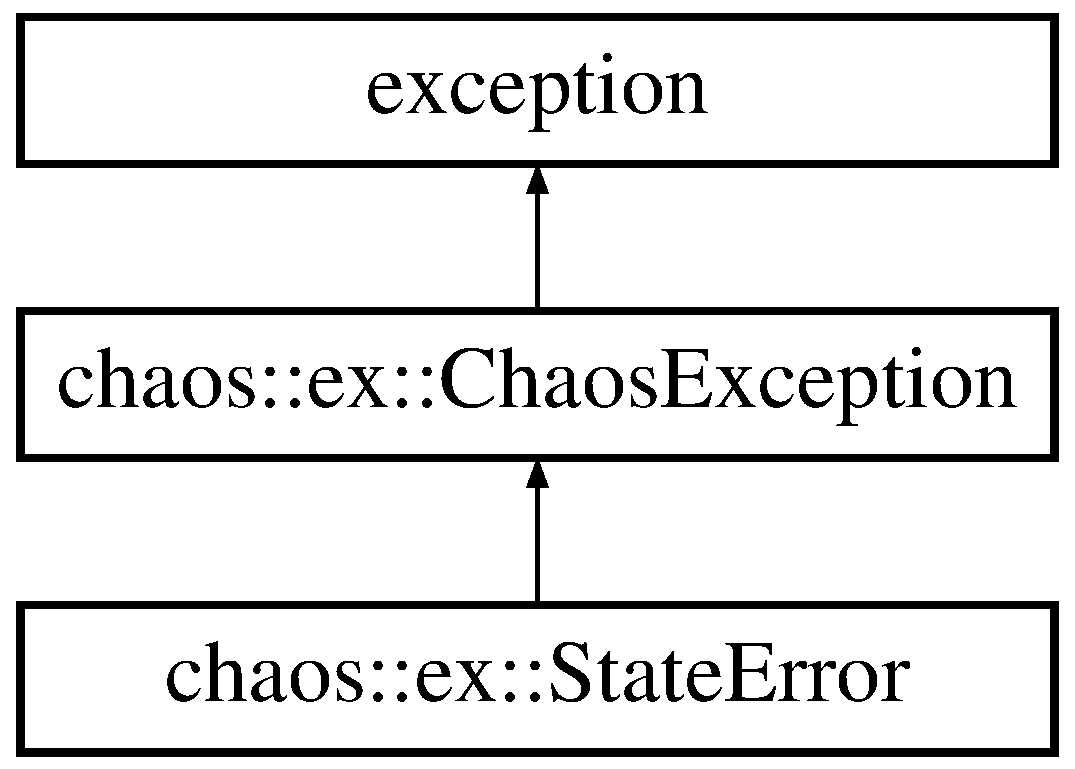
\includegraphics[height=3.000000cm]{classchaos_1_1ex_1_1_state_error}
\end{center}
\end{figure}
\subsection*{Public Member Functions}
\begin{DoxyCompactItemize}
\item 
\hypertarget{classchaos_1_1ex_1_1_state_error_abb2ed9dc030b7fbcb3c76a46d62da4ad}{{\bfseries State\-Error} (const \hyperlink{classchaos_1_1uni_1_1_u_t_f8_string}{chaos\-::uni\-::\-U\-T\-F8\-String} \&message)}\label{classchaos_1_1ex_1_1_state_error_abb2ed9dc030b7fbcb3c76a46d62da4ad}

\end{DoxyCompactItemize}
\subsection*{Additional Inherited Members}


\subsection{Detailed Description}
Warns that an action has been requested that is not valid for the current state. 

The documentation for this class was generated from the following file\-:\begin{DoxyCompactItemize}
\item 
/home/david/\-Dropbox/\-Development/\-Chaos\-Core/\-Chaos\-Core/src/cxx/chaoscore/base/\hyperlink{_base_exceptions_8hpp}{Base\-Exceptions.\-hpp}\end{DoxyCompactItemize}

\hypertarget{classchaos_1_1uni_1_1_u_t_f8_string}{\section{chaos\-:\-:uni\-:\-:U\-T\-F8\-String Class Reference}
\label{classchaos_1_1uni_1_1_u_t_f8_string}\index{chaos\-::uni\-::\-U\-T\-F8\-String@{chaos\-::uni\-::\-U\-T\-F8\-String}}
}


A string type designed for storing and manipulating U\-T\-F-\/8 encoded text.  




{\ttfamily \#include $<$U\-T\-F8\-String.\-hpp$>$}

\subsection*{Public Member Functions}
\begin{DoxyCompactItemize}
\item 
\hyperlink{classchaos_1_1uni_1_1_u_t_f8_string_a09647f0ade81a97ed55c75b9070b07a3}{U\-T\-F8\-String} ()
\begin{DoxyCompactList}\small\item\em Default constructor. \end{DoxyCompactList}\item 
\hyperlink{classchaos_1_1uni_1_1_u_t_f8_string_abb9cf9e655e1285179e47c698cfb1c56}{U\-T\-F8\-String} (const char $\ast$data)
\begin{DoxyCompactList}\small\item\em C style string constructor. \end{DoxyCompactList}\item 
\hyperlink{classchaos_1_1uni_1_1_u_t_f8_string_a2f9c060bed3206c69d2ab05f37e07b8c}{U\-T\-F8\-String} (const char $\ast$data, std\-::size\-\_\-t length)
\begin{DoxyCompactList}\small\item\em C style string and length constructor. \end{DoxyCompactList}\item 
\hyperlink{classchaos_1_1uni_1_1_u_t_f8_string_adabf7e6406a70581690a2b190143d01d}{U\-T\-F8\-String} (const \hyperlink{classchaos_1_1uni_1_1_u_t_f8_string}{U\-T\-F8\-String} \&other)
\begin{DoxyCompactList}\small\item\em Copy constructor. \end{DoxyCompactList}\item 
const \hyperlink{classchaos_1_1uni_1_1_u_t_f8_string}{U\-T\-F8\-String} \& \hyperlink{classchaos_1_1uni_1_1_u_t_f8_string_a9ff3d9661b17bbc979cc82d967c76c13}{operator=} (const \hyperlink{classchaos_1_1uni_1_1_u_t_f8_string}{U\-T\-F8\-String} \&other)
\begin{DoxyCompactList}\small\item\em Assignment operator. \end{DoxyCompactList}\item 
bool \hyperlink{classchaos_1_1uni_1_1_u_t_f8_string_af6f79ccd70af381eb6feba5fe3a3b2d0}{operator==} (const \hyperlink{classchaos_1_1uni_1_1_u_t_f8_string}{U\-T\-F8\-String} \&other) const 
\begin{DoxyCompactList}\small\item\em Equality operator. \end{DoxyCompactList}\item 
bool \hyperlink{classchaos_1_1uni_1_1_u_t_f8_string_ad2a48c9e0d16c41b64efae5b3c02d0a0}{operator!=} (const \hyperlink{classchaos_1_1uni_1_1_u_t_f8_string}{U\-T\-F8\-String} \&other) const 
\begin{DoxyCompactList}\small\item\em Inequality operator. \end{DoxyCompactList}\item 
bool \hyperlink{classchaos_1_1uni_1_1_u_t_f8_string_ad550d07d711ab6567d0ea91a18d403d0}{operator$<$} (const \hyperlink{classchaos_1_1uni_1_1_u_t_f8_string}{U\-T\-F8\-String} \&other) const 
\begin{DoxyCompactList}\small\item\em Less than operator. \end{DoxyCompactList}\item 
\hyperlink{classchaos_1_1uni_1_1_u_t_f8_string}{U\-T\-F8\-String} \hyperlink{classchaos_1_1uni_1_1_u_t_f8_string_a5fe1d0226ef6cb5517a57feb1b7f2170}{operator+} (const \hyperlink{classchaos_1_1uni_1_1_u_t_f8_string}{U\-T\-F8\-String} \&other) const 
\begin{DoxyCompactList}\small\item\em Addition operator. \end{DoxyCompactList}\item 
const \hyperlink{classchaos_1_1uni_1_1_u_t_f8_string}{U\-T\-F8\-String} \& \hyperlink{classchaos_1_1uni_1_1_u_t_f8_string_aeac2d47b0160a1d6ffee09c2078d940b}{operator+=} (const \hyperlink{classchaos_1_1uni_1_1_u_t_f8_string}{U\-T\-F8\-String} \&other)
\begin{DoxyCompactList}\small\item\em Compound addition operator. \end{DoxyCompactList}\item 
\hyperlink{classchaos_1_1uni_1_1_u_t_f8_string}{U\-T\-F8\-String} \hyperlink{classchaos_1_1uni_1_1_u_t_f8_string_ae281a6e92025aee3b31442574c3b335e}{operator$\ast$} (\hyperlink{namespacechaos_a8641b3ae4551f0b35570d4f9f4ec22d9}{chaos\-::uint32} count) const 
\begin{DoxyCompactList}\small\item\em Multiplication operator. \end{DoxyCompactList}\item 
const \hyperlink{classchaos_1_1uni_1_1_u_t_f8_string}{U\-T\-F8\-String} \& \hyperlink{classchaos_1_1uni_1_1_u_t_f8_string_a58a3e44978ba53fc9430e7361f36cec3}{operator$\ast$=} (\hyperlink{namespacechaos_a8641b3ae4551f0b35570d4f9f4ec22d9}{chaos\-::uint32} count)
\begin{DoxyCompactList}\small\item\em Compound multiplication operator. \end{DoxyCompactList}\item 
\hyperlink{classchaos_1_1uni_1_1_u_t_f8_string}{U\-T\-F8\-String} \& \hyperlink{classchaos_1_1uni_1_1_u_t_f8_string_a960cc1dcb7add75fb8dabd4bbc76980c}{operator$<$$<$} (const \hyperlink{classchaos_1_1uni_1_1_u_t_f8_string}{U\-T\-F8\-String} \&other)
\begin{DoxyCompactList}\small\item\em Stream operator. \end{DoxyCompactList}\item 
\hyperlink{classchaos_1_1uni_1_1_u_t_f8_string}{U\-T\-F8\-String} \& \hyperlink{classchaos_1_1uni_1_1_u_t_f8_string_a8282603511ed1a70804d7ec31105fb38}{operator$<$$<$} (const char $\ast$other)
\begin{DoxyCompactList}\small\item\em Stream operator. \end{DoxyCompactList}\item 
\hyperlink{classchaos_1_1uni_1_1_u_t_f8_string}{U\-T\-F8\-String} \& \hyperlink{classchaos_1_1uni_1_1_u_t_f8_string_aa347fb1d8e3e6e65ae37a52a2826854a}{operator$<$$<$} (const std\-::string \&other)
\begin{DoxyCompactList}\small\item\em Stream operator. \end{DoxyCompactList}\item 
\hyperlink{classchaos_1_1uni_1_1_u_t_f8_string}{U\-T\-F8\-String} \& \hyperlink{classchaos_1_1uni_1_1_u_t_f8_string_af9cfb931d9ab61aab0582911c6d1d5a4}{operator$<$$<$} (bool other)
\begin{DoxyCompactList}\small\item\em Stream operator. \end{DoxyCompactList}\item 
\hyperlink{classchaos_1_1uni_1_1_u_t_f8_string}{U\-T\-F8\-String} \& \hyperlink{classchaos_1_1uni_1_1_u_t_f8_string_a53fc209a9a929723baf6499911f1c9c3}{operator$<$$<$} (char other)
\begin{DoxyCompactList}\small\item\em Stream operator. \end{DoxyCompactList}\item 
\hyperlink{classchaos_1_1uni_1_1_u_t_f8_string}{U\-T\-F8\-String} \& \hyperlink{classchaos_1_1uni_1_1_u_t_f8_string_a003e6c1bc21fdf1af62d1e4e66ff9b38}{operator$<$$<$} (\hyperlink{namespacechaos_a557c5c30e5a935845432e60c617bd688}{chaos\-::int8} other)
\begin{DoxyCompactList}\small\item\em Stream operator. \end{DoxyCompactList}\item 
\hyperlink{classchaos_1_1uni_1_1_u_t_f8_string}{U\-T\-F8\-String} \& \hyperlink{classchaos_1_1uni_1_1_u_t_f8_string_af23b0ef36710e749e8ef6dd09e58c66c}{operator$<$$<$} (\hyperlink{namespacechaos_acbc0796d6929e3182cfd4f5c0176ab51}{chaos\-::uint8} other)
\begin{DoxyCompactList}\small\item\em Stream operator. \end{DoxyCompactList}\item 
\hyperlink{classchaos_1_1uni_1_1_u_t_f8_string}{U\-T\-F8\-String} \& \hyperlink{classchaos_1_1uni_1_1_u_t_f8_string_a614292b726bc437efdb129dad7819ab8}{operator$<$$<$} (\hyperlink{namespacechaos_a5dd2297d965311a05d313aaba7752f55}{chaos\-::int16} other)
\begin{DoxyCompactList}\small\item\em Stream operator. \end{DoxyCompactList}\item 
\hyperlink{classchaos_1_1uni_1_1_u_t_f8_string}{U\-T\-F8\-String} \& \hyperlink{classchaos_1_1uni_1_1_u_t_f8_string_a29ce72adbdee326e40c5906eb1511f86}{operator$<$$<$} (\hyperlink{namespacechaos_a7957eb5f7af90c890c4b14dfd3c95c5f}{chaos\-::uint16} other)
\begin{DoxyCompactList}\small\item\em Stream operator. \end{DoxyCompactList}\item 
\hyperlink{classchaos_1_1uni_1_1_u_t_f8_string}{U\-T\-F8\-String} \& \hyperlink{classchaos_1_1uni_1_1_u_t_f8_string_a9a4ae450649e6c7555497810b4878ab0}{operator$<$$<$} (\hyperlink{namespacechaos_aba819cd899114dc5873e32e7b26411c4}{chaos\-::int32} other)
\begin{DoxyCompactList}\small\item\em Stream operator. \end{DoxyCompactList}\item 
\hyperlink{classchaos_1_1uni_1_1_u_t_f8_string}{U\-T\-F8\-String} \& \hyperlink{classchaos_1_1uni_1_1_u_t_f8_string_a58bbad35225a1622e9593bafab6514ec}{operator$<$$<$} (\hyperlink{namespacechaos_a8641b3ae4551f0b35570d4f9f4ec22d9}{chaos\-::uint32} other)
\begin{DoxyCompactList}\small\item\em Stream operator. \end{DoxyCompactList}\item 
\hyperlink{classchaos_1_1uni_1_1_u_t_f8_string}{U\-T\-F8\-String} \& \hyperlink{classchaos_1_1uni_1_1_u_t_f8_string_a7b148a90a57870cf12735e3722992ac0}{operator$<$$<$} (\hyperlink{namespacechaos_aa4cfe70894188e01134a2694db2eb2db}{chaos\-::int64} other)
\begin{DoxyCompactList}\small\item\em Stream operator. \end{DoxyCompactList}\item 
\hyperlink{classchaos_1_1uni_1_1_u_t_f8_string}{U\-T\-F8\-String} \& \hyperlink{classchaos_1_1uni_1_1_u_t_f8_string_a45b9f65068486d6399c5bf9b88fbb021}{operator$<$$<$} (\hyperlink{namespacechaos_a9d62ad11fed4e3a5af70653b228ac910}{chaos\-::uint64} other)
\begin{DoxyCompactList}\small\item\em Stream operator. \end{DoxyCompactList}\item 
void \hyperlink{classchaos_1_1uni_1_1_u_t_f8_string_a87d1da629dd2a2071515e971fd5edffc}{assign} (const char $\ast$data)
\begin{DoxyCompactList}\small\item\em Assigns the internal data of this \hyperlink{classchaos_1_1uni_1_1_u_t_f8_string}{U\-T\-F8\-String} from the given C style string. \end{DoxyCompactList}\item 
void \hyperlink{classchaos_1_1uni_1_1_u_t_f8_string_a5c20ffede72bda70e6743de39aae7128}{assign} (const char $\ast$data, std\-::size\-\_\-t length)
\begin{DoxyCompactList}\small\item\em Assigns the internal data of this \hyperlink{classchaos_1_1uni_1_1_u_t_f8_string}{U\-T\-F8\-String} from the given C style string and byte length. \end{DoxyCompactList}\item 
void \hyperlink{classchaos_1_1uni_1_1_u_t_f8_string_af3e2f751444401ab7b5bc4c07b29de63}{assign} (const \hyperlink{classchaos_1_1uni_1_1_u_t_f8_string}{U\-T\-F8\-String} \&other)
\begin{DoxyCompactList}\small\item\em Assigns internal data from a copy of another \hyperlink{classchaos_1_1uni_1_1_u_t_f8_string}{U\-T\-F8\-String}. \end{DoxyCompactList}\item 
\hyperlink{classchaos_1_1uni_1_1_u_t_f8_string}{U\-T\-F8\-String} \& \hyperlink{classchaos_1_1uni_1_1_u_t_f8_string_a7d8ef533d14720da24ea4926daa2bc3f}{concatenate} (const \hyperlink{classchaos_1_1uni_1_1_u_t_f8_string}{U\-T\-F8\-String} \&other)
\begin{DoxyCompactList}\small\item\em Concatenates another \hyperlink{classchaos_1_1uni_1_1_u_t_f8_string}{U\-T\-F8\-String} on to the end of this string. \end{DoxyCompactList}\item 
\hyperlink{classchaos_1_1uni_1_1_u_t_f8_string}{U\-T\-F8\-String} \& \hyperlink{classchaos_1_1uni_1_1_u_t_f8_string_aae17e9b7d3522e4b504d7d0b5ec22b6e}{repeat} (\hyperlink{namespacechaos_a8641b3ae4551f0b35570d4f9f4ec22d9}{chaos\-::uint32} count)
\begin{DoxyCompactList}\small\item\em Extends this string with a copy of itself the given number of times. \end{DoxyCompactList}\item 
bool \hyperlink{classchaos_1_1uni_1_1_u_t_f8_string_aa4c4a2af7ab4fd921b47a3cb6942ce32}{starts\-\_\-with} (const \hyperlink{classchaos_1_1uni_1_1_u_t_f8_string}{U\-T\-F8\-String} \&\hyperlink{classchaos_1_1uni_1_1_u_t_f8_string_a6a92e0b096b7d0087e3c784fa7f891aa}{substring}) const 
\begin{DoxyCompactList}\small\item\em Checks whether this \hyperlink{classchaos_1_1uni_1_1_u_t_f8_string}{U\-T\-F8\-String} starts with the given substring. \end{DoxyCompactList}\item 
bool \hyperlink{classchaos_1_1uni_1_1_u_t_f8_string_abdf7eeafa6a476ea484d7a2a0e5060e5}{ends\-\_\-with} (const \hyperlink{classchaos_1_1uni_1_1_u_t_f8_string}{U\-T\-F8\-String} \&\hyperlink{classchaos_1_1uni_1_1_u_t_f8_string_a6a92e0b096b7d0087e3c784fa7f891aa}{substring}) const 
\begin{DoxyCompactList}\small\item\em Checks whether this \hyperlink{classchaos_1_1uni_1_1_u_t_f8_string}{U\-T\-F8\-String} ends with the given substring. \end{DoxyCompactList}\item 
std\-::size\-\_\-t \hyperlink{classchaos_1_1uni_1_1_u_t_f8_string_a45f75e01bd07e664369c81758a0f0537}{find\-\_\-first} (const \hyperlink{classchaos_1_1uni_1_1_u_t_f8_string}{U\-T\-F8\-String} \&\hyperlink{classchaos_1_1uni_1_1_u_t_f8_string_a6a92e0b096b7d0087e3c784fa7f891aa}{substring}) const 
\begin{DoxyCompactList}\small\item\em Finds the first occurrence of the given substring and returns the symbol index of it within this \hyperlink{classchaos_1_1uni_1_1_u_t_f8_string}{U\-T\-F8\-String}. \end{DoxyCompactList}\item 
std\-::size\-\_\-t \hyperlink{classchaos_1_1uni_1_1_u_t_f8_string_a482f2501d37379eab6661c45f13b0126}{find\-\_\-last} (const \hyperlink{classchaos_1_1uni_1_1_u_t_f8_string}{U\-T\-F8\-String} \&\hyperlink{classchaos_1_1uni_1_1_u_t_f8_string_a6a92e0b096b7d0087e3c784fa7f891aa}{substring}) const 
\begin{DoxyCompactList}\small\item\em Finds the last occurrence of the given substring and returns the index of it within this \hyperlink{classchaos_1_1uni_1_1_u_t_f8_string}{U\-T\-F8\-String}. \end{DoxyCompactList}\item 
const std\-::vector$<$ \hyperlink{classchaos_1_1uni_1_1_u_t_f8_string}{U\-T\-F8\-String} $>$ \hyperlink{classchaos_1_1uni_1_1_u_t_f8_string_a7d9a171234e75c018c2a0824f77222e7}{split} (const \hyperlink{classchaos_1_1uni_1_1_u_t_f8_string}{U\-T\-F8\-String} \&delimiter) const 
\begin{DoxyCompactList}\small\item\em Splits this \hyperlink{classchaos_1_1uni_1_1_u_t_f8_string}{U\-T\-F8\-String} by the given delimiter and returns the split elements in a std\-::vector. \end{DoxyCompactList}\item 
void \hyperlink{classchaos_1_1uni_1_1_u_t_f8_string_a940e7ccc70fe1d6c486a5a89941dd2ef}{remove\-\_\-duplicates} (const \hyperlink{classchaos_1_1uni_1_1_u_t_f8_string}{U\-T\-F8\-String} \&\hyperlink{classchaos_1_1uni_1_1_u_t_f8_string_a6a92e0b096b7d0087e3c784fa7f891aa}{substring})
\begin{DoxyCompactList}\small\item\em Removes consecutive duplicates of the given substring within this string. \end{DoxyCompactList}\item 
bool \hyperlink{classchaos_1_1uni_1_1_u_t_f8_string_a758102d22056ad004660c49104526642}{is\-\_\-int} () const 
\begin{DoxyCompactList}\small\item\em Whether the symbols of this string make up a valid integer type. \end{DoxyCompactList}\item 
bool \hyperlink{classchaos_1_1uni_1_1_u_t_f8_string_a0df001bc19b6ee2a9e843f88b82dbfe1}{is\-\_\-uint} () const 
\begin{DoxyCompactList}\small\item\em Whether the symbols of this string make up a valid unsigned integer type. \end{DoxyCompactList}\item 
bool \hyperlink{classchaos_1_1uni_1_1_u_t_f8_string_abc0b60f3ca6eff7782dc0e6a363ca919}{is\-\_\-float} () const 
\begin{DoxyCompactList}\small\item\em Whether the symbols of this string make up a valid floating point type. \end{DoxyCompactList}\item 
\hyperlink{classchaos_1_1uni_1_1_u_t_f8_string}{U\-T\-F8\-String} \hyperlink{classchaos_1_1uni_1_1_u_t_f8_string_a6a92e0b096b7d0087e3c784fa7f891aa}{substring} (std\-::size\-\_\-t start, std\-::size\-\_\-t length) const 
\begin{DoxyCompactList}\small\item\em Returns a new \hyperlink{classchaos_1_1uni_1_1_u_t_f8_string}{U\-T\-F8\-String} composed of a substring of this string. \end{DoxyCompactList}\item 
std\-::string \hyperlink{classchaos_1_1uni_1_1_u_t_f8_string_adbb12ac0c1ae8e1cb84b55cd8300fa55}{to\-\_\-std\-\_\-string} () const 
\begin{DoxyCompactList}\small\item\em Returns this as a standard library string. \end{DoxyCompactList}\item 
bool \hyperlink{classchaos_1_1uni_1_1_u_t_f8_string_a5c49dc0272b3eae0bb585b5f6ba03ad7}{to\-\_\-bool} () const 
\begin{DoxyCompactList}\small\item\em Returns this \hyperlink{classchaos_1_1uni_1_1_u_t_f8_string}{U\-T\-F8\-String} as an bool type. \end{DoxyCompactList}\item 
\hyperlink{namespacechaos_aba819cd899114dc5873e32e7b26411c4}{chaos\-::int32} \hyperlink{classchaos_1_1uni_1_1_u_t_f8_string_a743209e7c71e08c370267ae10b473ce0}{to\-\_\-int32} () const 
\begin{DoxyCompactList}\small\item\em Returns this \hyperlink{classchaos_1_1uni_1_1_u_t_f8_string}{U\-T\-F8\-String} as an int32 type. \end{DoxyCompactList}\item 
\hyperlink{namespacechaos_a8641b3ae4551f0b35570d4f9f4ec22d9}{chaos\-::uint32} \hyperlink{classchaos_1_1uni_1_1_u_t_f8_string_aa752c6db6c5a4f62c0c158d0bf7c0742}{to\-\_\-uint32} () const 
\begin{DoxyCompactList}\small\item\em Returns this \hyperlink{classchaos_1_1uni_1_1_u_t_f8_string}{U\-T\-F8\-String} as an uint32 type. \end{DoxyCompactList}\item 
\hyperlink{namespacechaos_aa4cfe70894188e01134a2694db2eb2db}{chaos\-::int64} \hyperlink{classchaos_1_1uni_1_1_u_t_f8_string_ac9db9e86ffa8572ba7ecf576d764d89f}{to\-\_\-int64} () const 
\begin{DoxyCompactList}\small\item\em Returns this \hyperlink{classchaos_1_1uni_1_1_u_t_f8_string}{U\-T\-F8\-String} as an int64 type. \end{DoxyCompactList}\item 
\hyperlink{namespacechaos_aa4cfe70894188e01134a2694db2eb2db}{chaos\-::int64} \hyperlink{classchaos_1_1uni_1_1_u_t_f8_string_afe8cb74c9fef1767790a33af2179a0b4}{to\-\_\-uint64} () const 
\begin{DoxyCompactList}\small\item\em Returns this \hyperlink{classchaos_1_1uni_1_1_u_t_f8_string}{U\-T\-F8\-String} as an uint64 type. \end{DoxyCompactList}\item 
std\-::size\-\_\-t \hyperlink{classchaos_1_1uni_1_1_u_t_f8_string_a9e0ec9cb771652c5ad61e2b54cf8b2aa}{get\-\_\-length} () const 
\begin{DoxyCompactList}\small\item\em Returns the number of symbols in this \hyperlink{classchaos_1_1uni_1_1_u_t_f8_string}{U\-T\-F8\-String}. \end{DoxyCompactList}\item 
bool \hyperlink{classchaos_1_1uni_1_1_u_t_f8_string_ad99ed42fcbd51651e6d626bab469af59}{is\-\_\-empty} () const 
\begin{DoxyCompactList}\small\item\em Returns whether the this \hyperlink{classchaos_1_1uni_1_1_u_t_f8_string}{U\-T\-F8\-String} contains any characters or not. \end{DoxyCompactList}\item 
\hyperlink{classchaos_1_1uni_1_1_u_t_f8_string}{U\-T\-F8\-String} \hyperlink{classchaos_1_1uni_1_1_u_t_f8_string_ae286e5ec21f22f709777dd7ecd55e05e}{get\-\_\-symbol} (std\-::size\-\_\-t index) const 
\begin{DoxyCompactList}\small\item\em Returns the U\-T\-F-\/8 symbol at the given index in this string. \end{DoxyCompactList}\item 
\hyperlink{namespacechaos_a8641b3ae4551f0b35570d4f9f4ec22d9}{chaos\-::uint32} \hyperlink{classchaos_1_1uni_1_1_u_t_f8_string_a2787c287f4fdaa0b4f2c1c7eccbf8f99}{get\-\_\-symbol\-\_\-value} (std\-::size\-\_\-t index=0) const 
\begin{DoxyCompactList}\small\item\em Returns the integer/hex value for the U\-T\-F-\/8 symbol at the given index in this string. \end{DoxyCompactList}\item 
\hyperlink{namespacechaos_a8641b3ae4551f0b35570d4f9f4ec22d9}{chaos\-::uint32} \hyperlink{classchaos_1_1uni_1_1_u_t_f8_string_a20b2a700379ac8ba32882d99b8a2a539}{get\-\_\-code\-\_\-point} (std\-::size\-\_\-t index=0) const 
\begin{DoxyCompactList}\small\item\em Returns the Unicode code point for the U\-T\-F-\/8 symbol at the given index in this string. \end{DoxyCompactList}\item 
std\-::size\-\_\-t \hyperlink{classchaos_1_1uni_1_1_u_t_f8_string_a1c8f623ae90b3ebbd28a95135e5c81f0}{get\-\_\-byte\-\_\-index\-\_\-for\-\_\-symbol\-\_\-index} (std\-::size\-\_\-t symbol\-\_\-index) const 
\begin{DoxyCompactList}\small\item\em Gets the index of the first byte for the symbol at the given index in this string. \end{DoxyCompactList}\item 
std\-::size\-\_\-t \hyperlink{classchaos_1_1uni_1_1_u_t_f8_string_a5043fb9645ef29de2b11b69186ec4132}{get\-\_\-symbol\-\_\-width} (std\-::size\-\_\-t index) const 
\begin{DoxyCompactList}\small\item\em Gets the number of bytes in the symbol at the given index in this string. \end{DoxyCompactList}\item 
const char $\ast$ \hyperlink{classchaos_1_1uni_1_1_u_t_f8_string_a91d3bb4cfbfb573b3fa6ecf3312f4dee}{get\-\_\-raw} () const 
\begin{DoxyCompactList}\small\item\em Gets the raw byte data of this \hyperlink{classchaos_1_1uni_1_1_u_t_f8_string}{U\-T\-F8\-String}. \end{DoxyCompactList}\item 
std\-::size\-\_\-t \hyperlink{classchaos_1_1uni_1_1_u_t_f8_string_a608a9a344875410a9b6e50d9ee0dbb65}{get\-\_\-byte\-\_\-length} () const 
\begin{DoxyCompactList}\small\item\em Returns the length of the internal data in bytes. \end{DoxyCompactList}\item 
std\-::size\-\_\-t \hyperlink{classchaos_1_1uni_1_1_u_t_f8_string_a89e9a1230821381e1d6d09099c119693}{get\-\_\-symbol\-\_\-index\-\_\-for\-\_\-byte\-\_\-index} (std\-::size\-\_\-t byte\-\_\-index) const 
\begin{DoxyCompactList}\small\item\em Returns the index of the symbol that the byte at the given index is part of. \end{DoxyCompactList}\item 
std\-::size\-\_\-t \hyperlink{classchaos_1_1uni_1_1_u_t_f8_string_ae0865f2a2dc39b4a9c3a7c968123f8fe}{get\-\_\-byte\-\_\-width} (std\-::size\-\_\-t byte\-\_\-index) const 
\begin{DoxyCompactList}\small\item\em Returns the number of bytes in the symbol at the given byte index. \end{DoxyCompactList}\end{DoxyCompactItemize}


\subsection{Detailed Description}
A string type designed for storing and manipulating U\-T\-F-\/8 encoded text. 

\begin{DoxyNote}{Note}
This object expects input text to already be U\-T\-F-\/8 encoded. For functions to convert encodings see \hyperlink{_unicode_operations_8hpp}{Unicode\-Operations.\-hpp}
\end{DoxyNote}
The \hyperlink{classchaos_1_1uni_1_1_u_t_f8_string}{U\-T\-F8\-String} data type is used extensively throughout Chaos\-Core and other Chaos Foundation projects.

Chaos\-Core stands by the principle that all string handling should be Unicode aware. The {\ttfamily char} primitive should only be used for storing and manipulation raw byte data, not for representing entire language characters. Furthermore Chaos\-Core considers U\-T\-F-\/8 to be the only default encoding type for Unicode text. Other encodings should only be used for special cases or interacting with applications that require a different encoding (such as the Windows A\-P\-I). For more info see \href{http://utf8everywhere.org/}{\tt http\-://utf8everywhere.\-org/}

For practicality the internal byte of an \hyperlink{classchaos_1_1uni_1_1_u_t_f8_string}{U\-T\-F8\-String} is N\-U\-L\-L terminated. This means the raw data can easily be used as native C style strings.

\begin{DoxyParagraph}{A Brief Introduction to U\-T\-F-\/8}

\end{DoxyParagraph}
In order to fully make use of the \hyperlink{classchaos_1_1uni_1_1_u_t_f8_string}{U\-T\-F8\-String} type's functionality its useful to understand the U\-T\-F-\/8 encoding method.

U\-T\-F-\/8 encodes each Unicode symbol in 1-\/4 bytes. The value of each symbol maps directly to a Unicode code point that represents the symbol. For example\-:


\begin{DoxyItemize}
\item \char`\"{}a\char`\"{} is stored using one byte with the hex value 0x61 or binary value {\ttfamily 01100001}
\item \char`\"{}ל\char`\"{} is stored using two bytes with the hex value 0x\-D79\-C or binary value {\ttfamily 11010111 10011100}
\item \char`\"{}∑\char`\"{} is stored using three bytes with the hex value 0x\-E28891 or binary value {\ttfamily 11100010 10001000 10010001}
\item \char`\"{}𝄞\char`\"{} is stored using four bytes with the hex value 0x\-F09\-D849\-E or binary value {\ttfamily 11110000 10011101 10000100 10011110}
\end{DoxyItemize}

The byte size of a U\-T\-F-\/8 symbol can be recognised by the bit pattern that makes up the start of each byte\-:


\begin{DoxyItemize}
\item One byte symbol\-: {\ttfamily 0xxxxxxx}
\item Two byte symbol\-: {\ttfamily 110xxxxx 10xxxxxx}
\item Three byte symbol\-: {\ttfamily 1110xxxx 10xxxxxx 10xxxxxx}
\item Four byte symbol\-: {\ttfamily 11110xxx 10xxxxxx 10xxxxxx 10xxxxxx}
\end{DoxyItemize}

\begin{DoxyParagraph}{U\-T\-F8\-String Usage}

\end{DoxyParagraph}
Here follows an example of using the \hyperlink{classchaos_1_1uni_1_1_u_t_f8_string}{U\-T\-F8\-String} type\-:

We have a C style string that cannot be encoded correctly with A\-S\-C\-I\-I (In this case we are assuming the input string is encoded in U\-T\-F-\/8)\-:


\begin{DoxyCode}
\textcolor{keyword}{const} \textcolor{keywordtype}{char}* cstring = \textcolor{stringliteral}{"aל∑"};
\end{DoxyCode}


If we inspect the length of the string we get unexpected results\-:


\begin{DoxyCode}
strlen( cstring );
\textcolor{comment}{// output: 6}
\end{DoxyCode}


This is because while the string only contains 3 symbols it contains 6 bytes which is what {\ttfamily strlen} is counting. Next we construct a \hyperlink{classchaos_1_1uni_1_1_u_t_f8_string}{U\-T\-F8\-String} using the c string data, and inspect it's length\-:


\begin{DoxyCode}
\hyperlink{classchaos_1_1uni_1_1_u_t_f8_string}{chaos::uni::UTF8String} utf8( cstring );
utf8.get\_length();
\textcolor{comment}{// output: 3}
utf8.get\_byte\_length()
\textcolor{comment}{// output: 6}
\end{DoxyCode}


\mbox{[}T\-O\-D\-O\-: iterator\mbox{]} We can now inspect each symbol in the string\-:


\begin{DoxyCode}
\textcolor{keywordflow}{for} ( std::size\_t i = 0; i < utf8.get\_length(); ++i )
\{
    \hyperlink{classchaos_1_1uni_1_1_u_t_f8_string}{chaos::uni::UTF8String} symbol( utf8.get\_symbol( i ) );
\}
\end{DoxyCode}


Note that the symbol is returned as an \hyperlink{classchaos_1_1uni_1_1_u_t_f8_string}{U\-T\-F8\-String} itself, this is due to the fact that symbol has a variable byte-\/width so cannot be stored in a {\ttfamily char}, nor is there any need to differentiate data types between a string of symbols and an individual symbol.

We can also inspect the byte-\/widths of each symbol in our string\-:


\begin{DoxyCode}
\textcolor{keywordflow}{for} ( std::size\_t i = 0; i < utf8.get\_length(); ++i )
\{
    utf8.get\_symbol\_width( i );
\}
\textcolor{comment}{// output: 1}
\textcolor{comment}{// output: 2}
\textcolor{comment}{// output: 3}
\end{DoxyCode}


The \hyperlink{classchaos_1_1uni_1_1_u_t_f8_string}{U\-T\-F8\-String} class provides many convenience functions for manipulating string data, such as {\ttfamily split}, {\ttfamily trim}, {\ttfamily starts\-\_\-with}, {\ttfamily find\-\_\-first}, {\ttfamily to\-\_\-raw}, {\ttfamily to\-\_\-stdstring}, etc.  

\subsection{Constructor \& Destructor Documentation}
\hypertarget{classchaos_1_1uni_1_1_u_t_f8_string_a09647f0ade81a97ed55c75b9070b07a3}{\index{chaos\-::uni\-::\-U\-T\-F8\-String@{chaos\-::uni\-::\-U\-T\-F8\-String}!U\-T\-F8\-String@{U\-T\-F8\-String}}
\index{U\-T\-F8\-String@{U\-T\-F8\-String}!chaos::uni::UTF8String@{chaos\-::uni\-::\-U\-T\-F8\-String}}
\subsubsection[{U\-T\-F8\-String}]{\setlength{\rightskip}{0pt plus 5cm}chaos\-::uni\-::\-U\-T\-F8\-String\-::\-U\-T\-F8\-String (
\begin{DoxyParamCaption}
{}
\end{DoxyParamCaption}
)}}\label{classchaos_1_1uni_1_1_u_t_f8_string_a09647f0ade81a97ed55c75b9070b07a3}


Default constructor. 

Creates a new \hyperlink{classchaos_1_1uni_1_1_u_t_f8_string}{U\-T\-F8\-String} that contains no symbols and holds only the N\-U\-L\-L terminator. \hypertarget{classchaos_1_1uni_1_1_u_t_f8_string_abb9cf9e655e1285179e47c698cfb1c56}{\index{chaos\-::uni\-::\-U\-T\-F8\-String@{chaos\-::uni\-::\-U\-T\-F8\-String}!U\-T\-F8\-String@{U\-T\-F8\-String}}
\index{U\-T\-F8\-String@{U\-T\-F8\-String}!chaos::uni::UTF8String@{chaos\-::uni\-::\-U\-T\-F8\-String}}
\subsubsection[{U\-T\-F8\-String}]{\setlength{\rightskip}{0pt plus 5cm}chaos\-::uni\-::\-U\-T\-F8\-String\-::\-U\-T\-F8\-String (
\begin{DoxyParamCaption}
\item[{const char $\ast$}]{data}
\end{DoxyParamCaption}
)}}\label{classchaos_1_1uni_1_1_u_t_f8_string_abb9cf9e655e1285179e47c698cfb1c56}


C style string constructor. 

Creates a new \hyperlink{classchaos_1_1uni_1_1_u_t_f8_string}{U\-T\-F8\-String} that contains the provided data.

\begin{DoxyNote}{Note}
The input data is expected to be U\-T\-F-\/8 encoded and N\-U\-L\-L terminated. For functions to convert encodings see \hyperlink{_unicode_operations_8hpp}{Unicode\-Operations.\-hpp} 
\end{DoxyNote}
\hypertarget{classchaos_1_1uni_1_1_u_t_f8_string_a2f9c060bed3206c69d2ab05f37e07b8c}{\index{chaos\-::uni\-::\-U\-T\-F8\-String@{chaos\-::uni\-::\-U\-T\-F8\-String}!U\-T\-F8\-String@{U\-T\-F8\-String}}
\index{U\-T\-F8\-String@{U\-T\-F8\-String}!chaos::uni::UTF8String@{chaos\-::uni\-::\-U\-T\-F8\-String}}
\subsubsection[{U\-T\-F8\-String}]{\setlength{\rightskip}{0pt plus 5cm}chaos\-::uni\-::\-U\-T\-F8\-String\-::\-U\-T\-F8\-String (
\begin{DoxyParamCaption}
\item[{const char $\ast$}]{data, }
\item[{std\-::size\-\_\-t}]{length}
\end{DoxyParamCaption}
)}}\label{classchaos_1_1uni_1_1_u_t_f8_string_a2f9c060bed3206c69d2ab05f37e07b8c}


C style string and length constructor. 

Creates a new \hyperlink{classchaos_1_1uni_1_1_u_t_f8_string}{U\-T\-F8\-String} using the given number of bytes from the data.

\begin{DoxyNote}{Note}
The input data is expected to be U\-T\-F-\/8 encoded but does not need to be N\-U\-L\-L terminated. For functions to convert encodings see \hyperlink{_unicode_operations_8hpp}{Unicode\-Operations.\-hpp}
\end{DoxyNote}

\begin{DoxyParams}{Parameters}
{\em data} & Character data to be used for this \hyperlink{classchaos_1_1uni_1_1_u_t_f8_string}{U\-T\-F8\-String}. \\
\hline
{\em length} & The number of bytes to read from the character data. \\
\hline
\end{DoxyParams}
\hypertarget{classchaos_1_1uni_1_1_u_t_f8_string_adabf7e6406a70581690a2b190143d01d}{\index{chaos\-::uni\-::\-U\-T\-F8\-String@{chaos\-::uni\-::\-U\-T\-F8\-String}!U\-T\-F8\-String@{U\-T\-F8\-String}}
\index{U\-T\-F8\-String@{U\-T\-F8\-String}!chaos::uni::UTF8String@{chaos\-::uni\-::\-U\-T\-F8\-String}}
\subsubsection[{U\-T\-F8\-String}]{\setlength{\rightskip}{0pt plus 5cm}chaos\-::uni\-::\-U\-T\-F8\-String\-::\-U\-T\-F8\-String (
\begin{DoxyParamCaption}
\item[{const {\bf U\-T\-F8\-String} \&}]{other}
\end{DoxyParamCaption}
)}}\label{classchaos_1_1uni_1_1_u_t_f8_string_adabf7e6406a70581690a2b190143d01d}


Copy constructor. 

Creates a new \hyperlink{classchaos_1_1uni_1_1_u_t_f8_string}{U\-T\-F8\-String} from a copy of the data from the given other \hyperlink{classchaos_1_1uni_1_1_u_t_f8_string}{U\-T\-F8\-String}. 

\subsection{Member Function Documentation}
\hypertarget{classchaos_1_1uni_1_1_u_t_f8_string_a9ff3d9661b17bbc979cc82d967c76c13}{\index{chaos\-::uni\-::\-U\-T\-F8\-String@{chaos\-::uni\-::\-U\-T\-F8\-String}!operator=@{operator=}}
\index{operator=@{operator=}!chaos::uni::UTF8String@{chaos\-::uni\-::\-U\-T\-F8\-String}}
\subsubsection[{operator=}]{\setlength{\rightskip}{0pt plus 5cm}const {\bf U\-T\-F8\-String}\& chaos\-::uni\-::\-U\-T\-F8\-String\-::operator= (
\begin{DoxyParamCaption}
\item[{const {\bf U\-T\-F8\-String} \&}]{other}
\end{DoxyParamCaption}
)}}\label{classchaos_1_1uni_1_1_u_t_f8_string_a9ff3d9661b17bbc979cc82d967c76c13}


Assignment operator. 

Assigns the internal of data this \hyperlink{classchaos_1_1uni_1_1_u_t_f8_string}{U\-T\-F8\-String} as a copy from the internal data of the provided \hyperlink{classchaos_1_1uni_1_1_u_t_f8_string}{U\-T\-F8\-String}.

Is the same as calling \hyperlink{classchaos_1_1uni_1_1_u_t_f8_string_af3e2f751444401ab7b5bc4c07b29de63}{assign( const U\-T\-F8\-String\& )}.


\begin{DoxyParams}{Parameters}
{\em other} & \hyperlink{classchaos_1_1uni_1_1_u_t_f8_string}{U\-T\-F8\-String} to copy internal data from. \\
\hline
\end{DoxyParams}
\begin{DoxyReturn}{Returns}
A reference to this \hyperlink{classchaos_1_1uni_1_1_u_t_f8_string}{U\-T\-F8\-String} after the assignment has taken place. 
\end{DoxyReturn}
\hypertarget{classchaos_1_1uni_1_1_u_t_f8_string_af6f79ccd70af381eb6feba5fe3a3b2d0}{\index{chaos\-::uni\-::\-U\-T\-F8\-String@{chaos\-::uni\-::\-U\-T\-F8\-String}!operator==@{operator==}}
\index{operator==@{operator==}!chaos::uni::UTF8String@{chaos\-::uni\-::\-U\-T\-F8\-String}}
\subsubsection[{operator==}]{\setlength{\rightskip}{0pt plus 5cm}bool chaos\-::uni\-::\-U\-T\-F8\-String\-::operator== (
\begin{DoxyParamCaption}
\item[{const {\bf U\-T\-F8\-String} \&}]{other}
\end{DoxyParamCaption}
) const}}\label{classchaos_1_1uni_1_1_u_t_f8_string_af6f79ccd70af381eb6feba5fe3a3b2d0}


Equality operator. 

Compares whether this \hyperlink{classchaos_1_1uni_1_1_u_t_f8_string}{U\-T\-F8\-String} and the other given \hyperlink{classchaos_1_1uni_1_1_u_t_f8_string}{U\-T\-F8\-String} are considered equal.


\begin{DoxyParams}{Parameters}
{\em other} & \hyperlink{classchaos_1_1uni_1_1_u_t_f8_string}{U\-T\-F8\-String} to compare this against. \\
\hline
\end{DoxyParams}
\begin{DoxyReturn}{Returns}
Whether the strings are equal. 
\end{DoxyReturn}
\hypertarget{classchaos_1_1uni_1_1_u_t_f8_string_ad2a48c9e0d16c41b64efae5b3c02d0a0}{\index{chaos\-::uni\-::\-U\-T\-F8\-String@{chaos\-::uni\-::\-U\-T\-F8\-String}!operator!=@{operator!=}}
\index{operator!=@{operator!=}!chaos::uni::UTF8String@{chaos\-::uni\-::\-U\-T\-F8\-String}}
\subsubsection[{operator!=}]{\setlength{\rightskip}{0pt plus 5cm}bool chaos\-::uni\-::\-U\-T\-F8\-String\-::operator!= (
\begin{DoxyParamCaption}
\item[{const {\bf U\-T\-F8\-String} \&}]{other}
\end{DoxyParamCaption}
) const}}\label{classchaos_1_1uni_1_1_u_t_f8_string_ad2a48c9e0d16c41b64efae5b3c02d0a0}


Inequality operator. 

Compares whether this \hyperlink{classchaos_1_1uni_1_1_u_t_f8_string}{U\-T\-F8\-String} and the other given \hyperlink{classchaos_1_1uni_1_1_u_t_f8_string}{U\-T\-F8\-String} are considered not equal. 
\begin{DoxyParams}{Parameters}
{\em other} & \hyperlink{classchaos_1_1uni_1_1_u_t_f8_string}{U\-T\-F8\-String} to compare this against. \\
\hline
\end{DoxyParams}
\begin{DoxyReturn}{Returns}
Whether the strings are not equal. 
\end{DoxyReturn}
\hypertarget{classchaos_1_1uni_1_1_u_t_f8_string_ad550d07d711ab6567d0ea91a18d403d0}{\index{chaos\-::uni\-::\-U\-T\-F8\-String@{chaos\-::uni\-::\-U\-T\-F8\-String}!operator$<$@{operator$<$}}
\index{operator$<$@{operator$<$}!chaos::uni::UTF8String@{chaos\-::uni\-::\-U\-T\-F8\-String}}
\subsubsection[{operator$<$}]{\setlength{\rightskip}{0pt plus 5cm}bool chaos\-::uni\-::\-U\-T\-F8\-String\-::operator$<$ (
\begin{DoxyParamCaption}
\item[{const {\bf U\-T\-F8\-String} \&}]{other}
\end{DoxyParamCaption}
) const}}\label{classchaos_1_1uni_1_1_u_t_f8_string_ad550d07d711ab6567d0ea91a18d403d0}


Less than operator. 

Compares whether this \hyperlink{classchaos_1_1uni_1_1_u_t_f8_string}{U\-T\-F8\-String} is less than the other given \hyperlink{classchaos_1_1uni_1_1_u_t_f8_string}{U\-T\-F8\-String}.

Less than is defined by performing a value comparison between each Unicode code point in the string.


\begin{DoxyParams}{Parameters}
{\em other} & \hyperlink{classchaos_1_1uni_1_1_u_t_f8_string}{U\-T\-F8\-String} to compare against. \\
\hline
\end{DoxyParams}
\begin{DoxyReturn}{Returns}
Whether this \hyperlink{classchaos_1_1uni_1_1_u_t_f8_string}{U\-T\-F8\-String} is less than the other. 
\end{DoxyReturn}
\hypertarget{classchaos_1_1uni_1_1_u_t_f8_string_a5fe1d0226ef6cb5517a57feb1b7f2170}{\index{chaos\-::uni\-::\-U\-T\-F8\-String@{chaos\-::uni\-::\-U\-T\-F8\-String}!operator+@{operator+}}
\index{operator+@{operator+}!chaos::uni::UTF8String@{chaos\-::uni\-::\-U\-T\-F8\-String}}
\subsubsection[{operator+}]{\setlength{\rightskip}{0pt plus 5cm}{\bf U\-T\-F8\-String} chaos\-::uni\-::\-U\-T\-F8\-String\-::operator+ (
\begin{DoxyParamCaption}
\item[{const {\bf U\-T\-F8\-String} \&}]{other}
\end{DoxyParamCaption}
) const}}\label{classchaos_1_1uni_1_1_u_t_f8_string_a5fe1d0226ef6cb5517a57feb1b7f2170}


Addition operator. 

Performs the same function as \hyperlink{classchaos_1_1uni_1_1_u_t_f8_string_a7d8ef533d14720da24ea4926daa2bc3f}{concatenate()} but does not cause any modifications to this string, instead returns a new string which contains the results of the concatenation.


\begin{DoxyParams}{Parameters}
{\em other} & \hyperlink{classchaos_1_1uni_1_1_u_t_f8_string}{U\-T\-F8\-String} to append to the end of a copy of this string. \\
\hline
\end{DoxyParams}
\begin{DoxyReturn}{Returns}
\hyperlink{classchaos_1_1uni_1_1_u_t_f8_string}{U\-T\-F8\-String} that contains the results of the concatenation. 
\end{DoxyReturn}
\hypertarget{classchaos_1_1uni_1_1_u_t_f8_string_aeac2d47b0160a1d6ffee09c2078d940b}{\index{chaos\-::uni\-::\-U\-T\-F8\-String@{chaos\-::uni\-::\-U\-T\-F8\-String}!operator+=@{operator+=}}
\index{operator+=@{operator+=}!chaos::uni::UTF8String@{chaos\-::uni\-::\-U\-T\-F8\-String}}
\subsubsection[{operator+=}]{\setlength{\rightskip}{0pt plus 5cm}const {\bf U\-T\-F8\-String}\& chaos\-::uni\-::\-U\-T\-F8\-String\-::operator+= (
\begin{DoxyParamCaption}
\item[{const {\bf U\-T\-F8\-String} \&}]{other}
\end{DoxyParamCaption}
)}}\label{classchaos_1_1uni_1_1_u_t_f8_string_aeac2d47b0160a1d6ffee09c2078d940b}


Compound addition operator. 

Performs the same function as \hyperlink{classchaos_1_1uni_1_1_u_t_f8_string_a7d8ef533d14720da24ea4926daa2bc3f}{concatenate()}.


\begin{DoxyParams}{Parameters}
{\em other} & \hyperlink{classchaos_1_1uni_1_1_u_t_f8_string}{U\-T\-F8\-String} to append to the end of this string. \\
\hline
\end{DoxyParams}
\begin{DoxyReturn}{Returns}
A reference to this \hyperlink{classchaos_1_1uni_1_1_u_t_f8_string}{U\-T\-F8\-String} after the concatenation has taken place. 
\end{DoxyReturn}
\hypertarget{classchaos_1_1uni_1_1_u_t_f8_string_ae281a6e92025aee3b31442574c3b335e}{\index{chaos\-::uni\-::\-U\-T\-F8\-String@{chaos\-::uni\-::\-U\-T\-F8\-String}!operator$\ast$@{operator$\ast$}}
\index{operator$\ast$@{operator$\ast$}!chaos::uni::UTF8String@{chaos\-::uni\-::\-U\-T\-F8\-String}}
\subsubsection[{operator$\ast$}]{\setlength{\rightskip}{0pt plus 5cm}{\bf U\-T\-F8\-String} chaos\-::uni\-::\-U\-T\-F8\-String\-::operator$\ast$ (
\begin{DoxyParamCaption}
\item[{{\bf chaos\-::uint32}}]{count}
\end{DoxyParamCaption}
) const}}\label{classchaos_1_1uni_1_1_u_t_f8_string_ae281a6e92025aee3b31442574c3b335e}


Multiplication operator. 

Performs the same function as \hyperlink{classchaos_1_1uni_1_1_u_t_f8_string_aae17e9b7d3522e4b504d7d0b5ec22b6e}{repeat()} but does not cause any modifications to this string, instead returns a new string which contains the results of the repeat.


\begin{DoxyParams}{Parameters}
{\em count} & the number of times to repeat the string \\
\hline
\end{DoxyParams}
\begin{DoxyReturn}{Returns}
\hyperlink{classchaos_1_1uni_1_1_u_t_f8_string}{U\-T\-F8\-String} that contains the results of the repeat. 
\end{DoxyReturn}
\hypertarget{classchaos_1_1uni_1_1_u_t_f8_string_a58a3e44978ba53fc9430e7361f36cec3}{\index{chaos\-::uni\-::\-U\-T\-F8\-String@{chaos\-::uni\-::\-U\-T\-F8\-String}!operator$\ast$=@{operator$\ast$=}}
\index{operator$\ast$=@{operator$\ast$=}!chaos::uni::UTF8String@{chaos\-::uni\-::\-U\-T\-F8\-String}}
\subsubsection[{operator$\ast$=}]{\setlength{\rightskip}{0pt plus 5cm}const {\bf U\-T\-F8\-String}\& chaos\-::uni\-::\-U\-T\-F8\-String\-::operator$\ast$= (
\begin{DoxyParamCaption}
\item[{{\bf chaos\-::uint32}}]{count}
\end{DoxyParamCaption}
)}}\label{classchaos_1_1uni_1_1_u_t_f8_string_a58a3e44978ba53fc9430e7361f36cec3}


Compound multiplication operator. 

Performs the same function as \hyperlink{classchaos_1_1uni_1_1_u_t_f8_string_aae17e9b7d3522e4b504d7d0b5ec22b6e}{repeat()}.


\begin{DoxyParams}{Parameters}
{\em count} & the number of times to repeat this string. \\
\hline
\end{DoxyParams}
\begin{DoxyReturn}{Returns}
A reference to this \hyperlink{classchaos_1_1uni_1_1_u_t_f8_string}{U\-T\-F8\-String} after the repeat operation has taken place. 
\end{DoxyReturn}
\hypertarget{classchaos_1_1uni_1_1_u_t_f8_string_a960cc1dcb7add75fb8dabd4bbc76980c}{\index{chaos\-::uni\-::\-U\-T\-F8\-String@{chaos\-::uni\-::\-U\-T\-F8\-String}!operator$<$$<$@{operator$<$$<$}}
\index{operator$<$$<$@{operator$<$$<$}!chaos::uni::UTF8String@{chaos\-::uni\-::\-U\-T\-F8\-String}}
\subsubsection[{operator$<$$<$}]{\setlength{\rightskip}{0pt plus 5cm}{\bf U\-T\-F8\-String}\& chaos\-::uni\-::\-U\-T\-F8\-String\-::operator$<$$<$ (
\begin{DoxyParamCaption}
\item[{const {\bf U\-T\-F8\-String} \&}]{other}
\end{DoxyParamCaption}
)}}\label{classchaos_1_1uni_1_1_u_t_f8_string_a960cc1dcb7add75fb8dabd4bbc76980c}


Stream operator. 

Extends this \hyperlink{classchaos_1_1uni_1_1_u_t_f8_string}{U\-T\-F8\-String} with the given other \hyperlink{classchaos_1_1uni_1_1_u_t_f8_string}{U\-T\-F8\-String}. \hypertarget{classchaos_1_1uni_1_1_u_t_f8_string_a8282603511ed1a70804d7ec31105fb38}{\index{chaos\-::uni\-::\-U\-T\-F8\-String@{chaos\-::uni\-::\-U\-T\-F8\-String}!operator$<$$<$@{operator$<$$<$}}
\index{operator$<$$<$@{operator$<$$<$}!chaos::uni::UTF8String@{chaos\-::uni\-::\-U\-T\-F8\-String}}
\subsubsection[{operator$<$$<$}]{\setlength{\rightskip}{0pt plus 5cm}{\bf U\-T\-F8\-String}\& chaos\-::uni\-::\-U\-T\-F8\-String\-::operator$<$$<$ (
\begin{DoxyParamCaption}
\item[{const char $\ast$}]{other}
\end{DoxyParamCaption}
)}}\label{classchaos_1_1uni_1_1_u_t_f8_string_a8282603511ed1a70804d7ec31105fb38}


Stream operator. 

Extends this \hyperlink{classchaos_1_1uni_1_1_u_t_f8_string}{U\-T\-F8\-String} with the given C style string.

\begin{DoxyNote}{Note}
The input data is expected to be U\-T\-F-\/8 encoded and N\-U\-L\-L terminated. For functions to convert encodings see \hyperlink{_unicode_operations_8hpp}{Unicode\-Operations.\-hpp} 
\end{DoxyNote}
\hypertarget{classchaos_1_1uni_1_1_u_t_f8_string_aa347fb1d8e3e6e65ae37a52a2826854a}{\index{chaos\-::uni\-::\-U\-T\-F8\-String@{chaos\-::uni\-::\-U\-T\-F8\-String}!operator$<$$<$@{operator$<$$<$}}
\index{operator$<$$<$@{operator$<$$<$}!chaos::uni::UTF8String@{chaos\-::uni\-::\-U\-T\-F8\-String}}
\subsubsection[{operator$<$$<$}]{\setlength{\rightskip}{0pt plus 5cm}{\bf U\-T\-F8\-String}\& chaos\-::uni\-::\-U\-T\-F8\-String\-::operator$<$$<$ (
\begin{DoxyParamCaption}
\item[{const std\-::string \&}]{other}
\end{DoxyParamCaption}
)}}\label{classchaos_1_1uni_1_1_u_t_f8_string_aa347fb1d8e3e6e65ae37a52a2826854a}


Stream operator. 

Extends this \hyperlink{classchaos_1_1uni_1_1_u_t_f8_string}{U\-T\-F8\-String} with the given std string.

\begin{DoxyNote}{Note}
The input data is expected to be U\-T\-F-\/8 encoded. For functions to convert encodings see \hyperlink{_unicode_operations_8hpp}{Unicode\-Operations.\-hpp} 
\end{DoxyNote}
\hypertarget{classchaos_1_1uni_1_1_u_t_f8_string_af9cfb931d9ab61aab0582911c6d1d5a4}{\index{chaos\-::uni\-::\-U\-T\-F8\-String@{chaos\-::uni\-::\-U\-T\-F8\-String}!operator$<$$<$@{operator$<$$<$}}
\index{operator$<$$<$@{operator$<$$<$}!chaos::uni::UTF8String@{chaos\-::uni\-::\-U\-T\-F8\-String}}
\subsubsection[{operator$<$$<$}]{\setlength{\rightskip}{0pt plus 5cm}{\bf U\-T\-F8\-String}\& chaos\-::uni\-::\-U\-T\-F8\-String\-::operator$<$$<$ (
\begin{DoxyParamCaption}
\item[{bool}]{other}
\end{DoxyParamCaption}
)}}\label{classchaos_1_1uni_1_1_u_t_f8_string_af9cfb931d9ab61aab0582911c6d1d5a4}


Stream operator. 

Extends this \hyperlink{classchaos_1_1uni_1_1_u_t_f8_string}{U\-T\-F8\-String} with the given boolean (where false = 0 and true = 1). \hypertarget{classchaos_1_1uni_1_1_u_t_f8_string_a53fc209a9a929723baf6499911f1c9c3}{\index{chaos\-::uni\-::\-U\-T\-F8\-String@{chaos\-::uni\-::\-U\-T\-F8\-String}!operator$<$$<$@{operator$<$$<$}}
\index{operator$<$$<$@{operator$<$$<$}!chaos::uni::UTF8String@{chaos\-::uni\-::\-U\-T\-F8\-String}}
\subsubsection[{operator$<$$<$}]{\setlength{\rightskip}{0pt plus 5cm}{\bf U\-T\-F8\-String}\& chaos\-::uni\-::\-U\-T\-F8\-String\-::operator$<$$<$ (
\begin{DoxyParamCaption}
\item[{char}]{other}
\end{DoxyParamCaption}
)}}\label{classchaos_1_1uni_1_1_u_t_f8_string_a53fc209a9a929723baf6499911f1c9c3}


Stream operator. 

Extends this \hyperlink{classchaos_1_1uni_1_1_u_t_f8_string}{U\-T\-F8\-String} with the given char. \hypertarget{classchaos_1_1uni_1_1_u_t_f8_string_a003e6c1bc21fdf1af62d1e4e66ff9b38}{\index{chaos\-::uni\-::\-U\-T\-F8\-String@{chaos\-::uni\-::\-U\-T\-F8\-String}!operator$<$$<$@{operator$<$$<$}}
\index{operator$<$$<$@{operator$<$$<$}!chaos::uni::UTF8String@{chaos\-::uni\-::\-U\-T\-F8\-String}}
\subsubsection[{operator$<$$<$}]{\setlength{\rightskip}{0pt plus 5cm}{\bf U\-T\-F8\-String}\& chaos\-::uni\-::\-U\-T\-F8\-String\-::operator$<$$<$ (
\begin{DoxyParamCaption}
\item[{{\bf chaos\-::int8}}]{other}
\end{DoxyParamCaption}
)}}\label{classchaos_1_1uni_1_1_u_t_f8_string_a003e6c1bc21fdf1af62d1e4e66ff9b38}


Stream operator. 

Extends this \hyperlink{classchaos_1_1uni_1_1_u_t_f8_string}{U\-T\-F8\-String} with the given int8. \hypertarget{classchaos_1_1uni_1_1_u_t_f8_string_af23b0ef36710e749e8ef6dd09e58c66c}{\index{chaos\-::uni\-::\-U\-T\-F8\-String@{chaos\-::uni\-::\-U\-T\-F8\-String}!operator$<$$<$@{operator$<$$<$}}
\index{operator$<$$<$@{operator$<$$<$}!chaos::uni::UTF8String@{chaos\-::uni\-::\-U\-T\-F8\-String}}
\subsubsection[{operator$<$$<$}]{\setlength{\rightskip}{0pt plus 5cm}{\bf U\-T\-F8\-String}\& chaos\-::uni\-::\-U\-T\-F8\-String\-::operator$<$$<$ (
\begin{DoxyParamCaption}
\item[{{\bf chaos\-::uint8}}]{other}
\end{DoxyParamCaption}
)}}\label{classchaos_1_1uni_1_1_u_t_f8_string_af23b0ef36710e749e8ef6dd09e58c66c}


Stream operator. 

Extends this \hyperlink{classchaos_1_1uni_1_1_u_t_f8_string}{U\-T\-F8\-String} with the given uint8. \hypertarget{classchaos_1_1uni_1_1_u_t_f8_string_a614292b726bc437efdb129dad7819ab8}{\index{chaos\-::uni\-::\-U\-T\-F8\-String@{chaos\-::uni\-::\-U\-T\-F8\-String}!operator$<$$<$@{operator$<$$<$}}
\index{operator$<$$<$@{operator$<$$<$}!chaos::uni::UTF8String@{chaos\-::uni\-::\-U\-T\-F8\-String}}
\subsubsection[{operator$<$$<$}]{\setlength{\rightskip}{0pt plus 5cm}{\bf U\-T\-F8\-String}\& chaos\-::uni\-::\-U\-T\-F8\-String\-::operator$<$$<$ (
\begin{DoxyParamCaption}
\item[{{\bf chaos\-::int16}}]{other}
\end{DoxyParamCaption}
)}}\label{classchaos_1_1uni_1_1_u_t_f8_string_a614292b726bc437efdb129dad7819ab8}


Stream operator. 

Extends this \hyperlink{classchaos_1_1uni_1_1_u_t_f8_string}{U\-T\-F8\-String} with the given int16. \hypertarget{classchaos_1_1uni_1_1_u_t_f8_string_a29ce72adbdee326e40c5906eb1511f86}{\index{chaos\-::uni\-::\-U\-T\-F8\-String@{chaos\-::uni\-::\-U\-T\-F8\-String}!operator$<$$<$@{operator$<$$<$}}
\index{operator$<$$<$@{operator$<$$<$}!chaos::uni::UTF8String@{chaos\-::uni\-::\-U\-T\-F8\-String}}
\subsubsection[{operator$<$$<$}]{\setlength{\rightskip}{0pt plus 5cm}{\bf U\-T\-F8\-String}\& chaos\-::uni\-::\-U\-T\-F8\-String\-::operator$<$$<$ (
\begin{DoxyParamCaption}
\item[{{\bf chaos\-::uint16}}]{other}
\end{DoxyParamCaption}
)}}\label{classchaos_1_1uni_1_1_u_t_f8_string_a29ce72adbdee326e40c5906eb1511f86}


Stream operator. 

Extends this \hyperlink{classchaos_1_1uni_1_1_u_t_f8_string}{U\-T\-F8\-String} with the given uint16. \hypertarget{classchaos_1_1uni_1_1_u_t_f8_string_a9a4ae450649e6c7555497810b4878ab0}{\index{chaos\-::uni\-::\-U\-T\-F8\-String@{chaos\-::uni\-::\-U\-T\-F8\-String}!operator$<$$<$@{operator$<$$<$}}
\index{operator$<$$<$@{operator$<$$<$}!chaos::uni::UTF8String@{chaos\-::uni\-::\-U\-T\-F8\-String}}
\subsubsection[{operator$<$$<$}]{\setlength{\rightskip}{0pt plus 5cm}{\bf U\-T\-F8\-String}\& chaos\-::uni\-::\-U\-T\-F8\-String\-::operator$<$$<$ (
\begin{DoxyParamCaption}
\item[{{\bf chaos\-::int32}}]{other}
\end{DoxyParamCaption}
)}}\label{classchaos_1_1uni_1_1_u_t_f8_string_a9a4ae450649e6c7555497810b4878ab0}


Stream operator. 

Extends this \hyperlink{classchaos_1_1uni_1_1_u_t_f8_string}{U\-T\-F8\-String} with the given int32. \hypertarget{classchaos_1_1uni_1_1_u_t_f8_string_a58bbad35225a1622e9593bafab6514ec}{\index{chaos\-::uni\-::\-U\-T\-F8\-String@{chaos\-::uni\-::\-U\-T\-F8\-String}!operator$<$$<$@{operator$<$$<$}}
\index{operator$<$$<$@{operator$<$$<$}!chaos::uni::UTF8String@{chaos\-::uni\-::\-U\-T\-F8\-String}}
\subsubsection[{operator$<$$<$}]{\setlength{\rightskip}{0pt plus 5cm}{\bf U\-T\-F8\-String}\& chaos\-::uni\-::\-U\-T\-F8\-String\-::operator$<$$<$ (
\begin{DoxyParamCaption}
\item[{{\bf chaos\-::uint32}}]{other}
\end{DoxyParamCaption}
)}}\label{classchaos_1_1uni_1_1_u_t_f8_string_a58bbad35225a1622e9593bafab6514ec}


Stream operator. 

Extends this \hyperlink{classchaos_1_1uni_1_1_u_t_f8_string}{U\-T\-F8\-String} with the given unsigned int32. \hypertarget{classchaos_1_1uni_1_1_u_t_f8_string_a7b148a90a57870cf12735e3722992ac0}{\index{chaos\-::uni\-::\-U\-T\-F8\-String@{chaos\-::uni\-::\-U\-T\-F8\-String}!operator$<$$<$@{operator$<$$<$}}
\index{operator$<$$<$@{operator$<$$<$}!chaos::uni::UTF8String@{chaos\-::uni\-::\-U\-T\-F8\-String}}
\subsubsection[{operator$<$$<$}]{\setlength{\rightskip}{0pt plus 5cm}{\bf U\-T\-F8\-String}\& chaos\-::uni\-::\-U\-T\-F8\-String\-::operator$<$$<$ (
\begin{DoxyParamCaption}
\item[{{\bf chaos\-::int64}}]{other}
\end{DoxyParamCaption}
)}}\label{classchaos_1_1uni_1_1_u_t_f8_string_a7b148a90a57870cf12735e3722992ac0}


Stream operator. 

Extends this \hyperlink{classchaos_1_1uni_1_1_u_t_f8_string}{U\-T\-F8\-String} with the given int64. \hypertarget{classchaos_1_1uni_1_1_u_t_f8_string_a45b9f65068486d6399c5bf9b88fbb021}{\index{chaos\-::uni\-::\-U\-T\-F8\-String@{chaos\-::uni\-::\-U\-T\-F8\-String}!operator$<$$<$@{operator$<$$<$}}
\index{operator$<$$<$@{operator$<$$<$}!chaos::uni::UTF8String@{chaos\-::uni\-::\-U\-T\-F8\-String}}
\subsubsection[{operator$<$$<$}]{\setlength{\rightskip}{0pt plus 5cm}{\bf U\-T\-F8\-String}\& chaos\-::uni\-::\-U\-T\-F8\-String\-::operator$<$$<$ (
\begin{DoxyParamCaption}
\item[{{\bf chaos\-::uint64}}]{other}
\end{DoxyParamCaption}
)}}\label{classchaos_1_1uni_1_1_u_t_f8_string_a45b9f65068486d6399c5bf9b88fbb021}


Stream operator. 

Extends this \hyperlink{classchaos_1_1uni_1_1_u_t_f8_string}{U\-T\-F8\-String} with the given unsigned int64. \hypertarget{classchaos_1_1uni_1_1_u_t_f8_string_a87d1da629dd2a2071515e971fd5edffc}{\index{chaos\-::uni\-::\-U\-T\-F8\-String@{chaos\-::uni\-::\-U\-T\-F8\-String}!assign@{assign}}
\index{assign@{assign}!chaos::uni::UTF8String@{chaos\-::uni\-::\-U\-T\-F8\-String}}
\subsubsection[{assign}]{\setlength{\rightskip}{0pt plus 5cm}void chaos\-::uni\-::\-U\-T\-F8\-String\-::assign (
\begin{DoxyParamCaption}
\item[{const char $\ast$}]{data}
\end{DoxyParamCaption}
)}}\label{classchaos_1_1uni_1_1_u_t_f8_string_a87d1da629dd2a2071515e971fd5edffc}


Assigns the internal data of this \hyperlink{classchaos_1_1uni_1_1_u_t_f8_string}{U\-T\-F8\-String} from the given C style string. 

This operation will delete any current internal data of this \hyperlink{classchaos_1_1uni_1_1_u_t_f8_string}{U\-T\-F8\-String}.

\begin{DoxyNote}{Note}
The input data is expected to be U\-T\-F-\/8 encoded and N\-U\-L\-L terminated. For functions to convert encodings see \hyperlink{_unicode_operations_8hpp}{Unicode\-Operations.\-hpp} 
\end{DoxyNote}
\hypertarget{classchaos_1_1uni_1_1_u_t_f8_string_a5c20ffede72bda70e6743de39aae7128}{\index{chaos\-::uni\-::\-U\-T\-F8\-String@{chaos\-::uni\-::\-U\-T\-F8\-String}!assign@{assign}}
\index{assign@{assign}!chaos::uni::UTF8String@{chaos\-::uni\-::\-U\-T\-F8\-String}}
\subsubsection[{assign}]{\setlength{\rightskip}{0pt plus 5cm}void chaos\-::uni\-::\-U\-T\-F8\-String\-::assign (
\begin{DoxyParamCaption}
\item[{const char $\ast$}]{data, }
\item[{std\-::size\-\_\-t}]{length}
\end{DoxyParamCaption}
)}}\label{classchaos_1_1uni_1_1_u_t_f8_string_a5c20ffede72bda70e6743de39aae7128}


Assigns the internal data of this \hyperlink{classchaos_1_1uni_1_1_u_t_f8_string}{U\-T\-F8\-String} from the given C style string and byte length. 

Creates a new \hyperlink{classchaos_1_1uni_1_1_u_t_f8_string}{U\-T\-F8\-String} using the given number of bytes from the data. This operation will delete any current internal data of this \hyperlink{classchaos_1_1uni_1_1_u_t_f8_string}{U\-T\-F8\-String}.

\begin{DoxyNote}{Note}
The input data is expected to be U\-T\-F-\/8 encoded but does not need to be N\-U\-L\-L terminated. For functions to convert encodings see \hyperlink{_unicode_operations_8hpp}{Unicode\-Operations.\-hpp}
\end{DoxyNote}

\begin{DoxyParams}{Parameters}
{\em data} & Character data to be used for this \hyperlink{classchaos_1_1uni_1_1_u_t_f8_string}{U\-T\-F8\-String}. \\
\hline
{\em length} & The number of bytes to read from the character data. \\
\hline
\end{DoxyParams}
\hypertarget{classchaos_1_1uni_1_1_u_t_f8_string_af3e2f751444401ab7b5bc4c07b29de63}{\index{chaos\-::uni\-::\-U\-T\-F8\-String@{chaos\-::uni\-::\-U\-T\-F8\-String}!assign@{assign}}
\index{assign@{assign}!chaos::uni::UTF8String@{chaos\-::uni\-::\-U\-T\-F8\-String}}
\subsubsection[{assign}]{\setlength{\rightskip}{0pt plus 5cm}void chaos\-::uni\-::\-U\-T\-F8\-String\-::assign (
\begin{DoxyParamCaption}
\item[{const {\bf U\-T\-F8\-String} \&}]{other}
\end{DoxyParamCaption}
)}}\label{classchaos_1_1uni_1_1_u_t_f8_string_af3e2f751444401ab7b5bc4c07b29de63}


Assigns internal data from a copy of another \hyperlink{classchaos_1_1uni_1_1_u_t_f8_string}{U\-T\-F8\-String}. 

This operation will delete any current internal data of this \hyperlink{classchaos_1_1uni_1_1_u_t_f8_string}{U\-T\-F8\-String}. \hypertarget{classchaos_1_1uni_1_1_u_t_f8_string_a7d8ef533d14720da24ea4926daa2bc3f}{\index{chaos\-::uni\-::\-U\-T\-F8\-String@{chaos\-::uni\-::\-U\-T\-F8\-String}!concatenate@{concatenate}}
\index{concatenate@{concatenate}!chaos::uni::UTF8String@{chaos\-::uni\-::\-U\-T\-F8\-String}}
\subsubsection[{concatenate}]{\setlength{\rightskip}{0pt plus 5cm}{\bf U\-T\-F8\-String}\& chaos\-::uni\-::\-U\-T\-F8\-String\-::concatenate (
\begin{DoxyParamCaption}
\item[{const {\bf U\-T\-F8\-String} \&}]{other}
\end{DoxyParamCaption}
)}}\label{classchaos_1_1uni_1_1_u_t_f8_string_a7d8ef533d14720da24ea4926daa2bc3f}


Concatenates another \hyperlink{classchaos_1_1uni_1_1_u_t_f8_string}{U\-T\-F8\-String} on to the end of this string. 

\begin{DoxyNote}{Note}
This operation modifies this \hyperlink{classchaos_1_1uni_1_1_u_t_f8_string}{U\-T\-F8\-String}.
\end{DoxyNote}
Example usage\-:


\begin{DoxyCode}
\hyperlink{classchaos_1_1uni_1_1_u_t_f8_string}{chaos::uni::UTF8String} s\_1( \textcolor{stringliteral}{"Hello"} );
\hyperlink{classchaos_1_1uni_1_1_u_t_f8_string}{chaos::uni::UTF8String} s\_2( \textcolor{stringliteral}{"World"} );
s\_1.concatenate( s\_2 );
std::cout << s\_1 << std::endl;
\textcolor{comment}{// output: Hello World}
\end{DoxyCode}


\hyperlink{classchaos_1_1uni_1_1_u_t_f8_string}{U\-T\-F8\-String} to append to the end of this string. \begin{DoxyReturn}{Returns}
A reference to this \hyperlink{classchaos_1_1uni_1_1_u_t_f8_string}{U\-T\-F8\-String} after the concatenation has taken place. 
\end{DoxyReturn}
\hypertarget{classchaos_1_1uni_1_1_u_t_f8_string_aae17e9b7d3522e4b504d7d0b5ec22b6e}{\index{chaos\-::uni\-::\-U\-T\-F8\-String@{chaos\-::uni\-::\-U\-T\-F8\-String}!repeat@{repeat}}
\index{repeat@{repeat}!chaos::uni::UTF8String@{chaos\-::uni\-::\-U\-T\-F8\-String}}
\subsubsection[{repeat}]{\setlength{\rightskip}{0pt plus 5cm}{\bf U\-T\-F8\-String}\& chaos\-::uni\-::\-U\-T\-F8\-String\-::repeat (
\begin{DoxyParamCaption}
\item[{{\bf chaos\-::uint32}}]{count}
\end{DoxyParamCaption}
)}}\label{classchaos_1_1uni_1_1_u_t_f8_string_aae17e9b7d3522e4b504d7d0b5ec22b6e}


Extends this string with a copy of itself the given number of times. 

\begin{DoxyNote}{Note}
This operation modifies this \hyperlink{classchaos_1_1uni_1_1_u_t_f8_string}{U\-T\-F8\-String}.
\end{DoxyNote}
Example usage\-:


\begin{DoxyCode}
\hyperlink{classchaos_1_1uni_1_1_u_t_f8_string}{chaos::uni::UTF8String} s( \textcolor{stringliteral}{"Hello"} );
s.\hyperlink{classchaos_1_1uni_1_1_u_t_f8_string_aae17e9b7d3522e4b504d7d0b5ec22b6e}{repeat}( 3 );
std::cout << s << std::endl;
\textcolor{comment}{// output: HelloHelloHello}
\end{DoxyCode}



\begin{DoxyParams}{Parameters}
{\em count} & The number of times to repeat this string. \\
\hline
\end{DoxyParams}
\begin{DoxyReturn}{Returns}
A reference to this \hyperlink{classchaos_1_1uni_1_1_u_t_f8_string}{U\-T\-F8\-String} after repeat has taken place. 
\end{DoxyReturn}
\hypertarget{classchaos_1_1uni_1_1_u_t_f8_string_aa4c4a2af7ab4fd921b47a3cb6942ce32}{\index{chaos\-::uni\-::\-U\-T\-F8\-String@{chaos\-::uni\-::\-U\-T\-F8\-String}!starts\-\_\-with@{starts\-\_\-with}}
\index{starts\-\_\-with@{starts\-\_\-with}!chaos::uni::UTF8String@{chaos\-::uni\-::\-U\-T\-F8\-String}}
\subsubsection[{starts\-\_\-with}]{\setlength{\rightskip}{0pt plus 5cm}bool chaos\-::uni\-::\-U\-T\-F8\-String\-::starts\-\_\-with (
\begin{DoxyParamCaption}
\item[{const {\bf U\-T\-F8\-String} \&}]{substring}
\end{DoxyParamCaption}
) const}}\label{classchaos_1_1uni_1_1_u_t_f8_string_aa4c4a2af7ab4fd921b47a3cb6942ce32}


Checks whether this \hyperlink{classchaos_1_1uni_1_1_u_t_f8_string}{U\-T\-F8\-String} starts with the given substring. 

Example usage\-:


\begin{DoxyCode}
\hyperlink{classchaos_1_1uni_1_1_u_t_f8_string}{chaos::uni::UTF8String} s\_1( \textcolor{stringliteral}{"Hello World"} );
\hyperlink{classchaos_1_1uni_1_1_u_t_f8_string}{chaos::uni::UTF8String} s\_2( \textcolor{stringliteral}{"Hello"} );
\hyperlink{classchaos_1_1uni_1_1_u_t_f8_string}{chaos::uni::UTF8String} s\_3( \textcolor{stringliteral}{"World"} );
s\_1.starts\_with( s\_2 ); \textcolor{comment}{// returns: true}
s\_1.starts\_with( s\_3 ); \textcolor{comment}{// returns: false}
\end{DoxyCode}
 \hypertarget{classchaos_1_1uni_1_1_u_t_f8_string_abdf7eeafa6a476ea484d7a2a0e5060e5}{\index{chaos\-::uni\-::\-U\-T\-F8\-String@{chaos\-::uni\-::\-U\-T\-F8\-String}!ends\-\_\-with@{ends\-\_\-with}}
\index{ends\-\_\-with@{ends\-\_\-with}!chaos::uni::UTF8String@{chaos\-::uni\-::\-U\-T\-F8\-String}}
\subsubsection[{ends\-\_\-with}]{\setlength{\rightskip}{0pt plus 5cm}bool chaos\-::uni\-::\-U\-T\-F8\-String\-::ends\-\_\-with (
\begin{DoxyParamCaption}
\item[{const {\bf U\-T\-F8\-String} \&}]{substring}
\end{DoxyParamCaption}
) const}}\label{classchaos_1_1uni_1_1_u_t_f8_string_abdf7eeafa6a476ea484d7a2a0e5060e5}


Checks whether this \hyperlink{classchaos_1_1uni_1_1_u_t_f8_string}{U\-T\-F8\-String} ends with the given substring. 

Example usage\-:


\begin{DoxyCode}
\hyperlink{classchaos_1_1uni_1_1_u_t_f8_string}{chaos::uni::UTF8String} s\_1( \textcolor{stringliteral}{"Hello World"} );
\hyperlink{classchaos_1_1uni_1_1_u_t_f8_string}{chaos::uni::UTF8String} s\_2( \textcolor{stringliteral}{"Hello"} );
\hyperlink{classchaos_1_1uni_1_1_u_t_f8_string}{chaos::uni::UTF8String} s\_3( \textcolor{stringliteral}{"World"} );
s\_1.ends\_with( s\_2 ); \textcolor{comment}{// returns: false}
s\_1.ends\_with( s\_3 ); \textcolor{comment}{// returns: true}
\end{DoxyCode}
 \hypertarget{classchaos_1_1uni_1_1_u_t_f8_string_a45f75e01bd07e664369c81758a0f0537}{\index{chaos\-::uni\-::\-U\-T\-F8\-String@{chaos\-::uni\-::\-U\-T\-F8\-String}!find\-\_\-first@{find\-\_\-first}}
\index{find\-\_\-first@{find\-\_\-first}!chaos::uni::UTF8String@{chaos\-::uni\-::\-U\-T\-F8\-String}}
\subsubsection[{find\-\_\-first}]{\setlength{\rightskip}{0pt plus 5cm}std\-::size\-\_\-t chaos\-::uni\-::\-U\-T\-F8\-String\-::find\-\_\-first (
\begin{DoxyParamCaption}
\item[{const {\bf U\-T\-F8\-String} \&}]{substring}
\end{DoxyParamCaption}
) const}}\label{classchaos_1_1uni_1_1_u_t_f8_string_a45f75e01bd07e664369c81758a0f0537}


Finds the first occurrence of the given substring and returns the symbol index of it within this \hyperlink{classchaos_1_1uni_1_1_u_t_f8_string}{U\-T\-F8\-String}. 

Example usage\-:


\begin{DoxyCode}
\hyperlink{classchaos_1_1uni_1_1_u_t_f8_string}{chaos::uni::UTF8String} s\_1( \textcolor{stringliteral}{"Hello World"} );
\hyperlink{classchaos_1_1uni_1_1_u_t_f8_string}{chaos::uni::UTF8String} s\_2( \textcolor{stringliteral}{"World"} );
\hyperlink{classchaos_1_1uni_1_1_u_t_f8_string}{chaos::uni::UTF8String} s\_3( \textcolor{stringliteral}{"*"} );
s\_1.find\_first( s\_2 ); \textcolor{comment}{// returns: 6}
s\_1.find\_first( s\_3 ); \textcolor{comment}{// returns: chaos::uni::npos}
\end{DoxyCode}



\begin{DoxyParams}{Parameters}
{\em substring} & \hyperlink{classchaos_1_1uni_1_1_u_t_f8_string}{U\-T\-F8\-String} to find the first occurrence of in this string. \\
\hline
\end{DoxyParams}
\begin{DoxyReturn}{Returns}
The index of the beginning of the first occurrence of the substring in this string. If the substring could not be found, \hyperlink{namespacechaos_1_1uni_af28f3dcb2b4845d8a39b3d16e86c174b}{chaos\-::uni\-::npos} is returned instead. 
\end{DoxyReturn}
\hypertarget{classchaos_1_1uni_1_1_u_t_f8_string_a482f2501d37379eab6661c45f13b0126}{\index{chaos\-::uni\-::\-U\-T\-F8\-String@{chaos\-::uni\-::\-U\-T\-F8\-String}!find\-\_\-last@{find\-\_\-last}}
\index{find\-\_\-last@{find\-\_\-last}!chaos::uni::UTF8String@{chaos\-::uni\-::\-U\-T\-F8\-String}}
\subsubsection[{find\-\_\-last}]{\setlength{\rightskip}{0pt plus 5cm}std\-::size\-\_\-t chaos\-::uni\-::\-U\-T\-F8\-String\-::find\-\_\-last (
\begin{DoxyParamCaption}
\item[{const {\bf U\-T\-F8\-String} \&}]{substring}
\end{DoxyParamCaption}
) const}}\label{classchaos_1_1uni_1_1_u_t_f8_string_a482f2501d37379eab6661c45f13b0126}


Finds the last occurrence of the given substring and returns the index of it within this \hyperlink{classchaos_1_1uni_1_1_u_t_f8_string}{U\-T\-F8\-String}. 

Example usage\-:


\begin{DoxyCode}
\hyperlink{classchaos_1_1uni_1_1_u_t_f8_string}{chaos::uni::UTF8String} s\_1( \textcolor{stringliteral}{"Hello World World"} );
\hyperlink{classchaos_1_1uni_1_1_u_t_f8_string}{chaos::uni::UTF8String} s\_2( \textcolor{stringliteral}{"World"} );
\hyperlink{classchaos_1_1uni_1_1_u_t_f8_string}{chaos::uni::UTF8String} s\_3( \textcolor{stringliteral}{"*"} );
s\_1.find\_first( s\_2 ); \textcolor{comment}{// returns: 12}
s\_1.find\_first( s\_3 ); \textcolor{comment}{// returns: chaos::uni::npos}
\end{DoxyCode}



\begin{DoxyParams}{Parameters}
{\em substring} & \hyperlink{classchaos_1_1uni_1_1_u_t_f8_string}{U\-T\-F8\-String} to find the last occurrence of in this string. \\
\hline
\end{DoxyParams}
\begin{DoxyReturn}{Returns}
The index of the beginning of the last occurrence of the substring in this string. If the substring could not be found, \hyperlink{namespacechaos_1_1uni_af28f3dcb2b4845d8a39b3d16e86c174b}{chaos\-::uni\-::npos} is returned instead. 
\end{DoxyReturn}
\hypertarget{classchaos_1_1uni_1_1_u_t_f8_string_a7d9a171234e75c018c2a0824f77222e7}{\index{chaos\-::uni\-::\-U\-T\-F8\-String@{chaos\-::uni\-::\-U\-T\-F8\-String}!split@{split}}
\index{split@{split}!chaos::uni::UTF8String@{chaos\-::uni\-::\-U\-T\-F8\-String}}
\subsubsection[{split}]{\setlength{\rightskip}{0pt plus 5cm}const std\-::vector$<$ {\bf U\-T\-F8\-String} $>$ chaos\-::uni\-::\-U\-T\-F8\-String\-::split (
\begin{DoxyParamCaption}
\item[{const {\bf U\-T\-F8\-String} \&}]{delimiter}
\end{DoxyParamCaption}
) const}}\label{classchaos_1_1uni_1_1_u_t_f8_string_a7d9a171234e75c018c2a0824f77222e7}


Splits this \hyperlink{classchaos_1_1uni_1_1_u_t_f8_string}{U\-T\-F8\-String} by the given delimiter and returns the split elements in a std\-::vector. 

Example usage\-:


\begin{DoxyCode}
\hyperlink{classchaos_1_1uni_1_1_u_t_f8_string}{chaos::uni::UTF8String} s( \textcolor{stringliteral}{"Hello\_World"} );
\hyperlink{classchaos_1_1uni_1_1_u_t_f8_string}{chaos::uni::UTF8String} delim( \textcolor{stringliteral}{"\_"} );
std::vector< chaos::uni::UTF8String > elements = s.\hyperlink{classchaos_1_1uni_1_1_u_t_f8_string_a7d9a171234e75c018c2a0824f77222e7}{split}( delim );
\textcolor{comment}{// vector contents: [ "Hello", "World" ]}
\end{DoxyCode}



\begin{DoxyExceptions}{Exceptions}
{\em \hyperlink{classchaos_1_1ex_1_1_value_error}{chaos\-::ex\-::\-Value\-Error}} & If the provided delimiter is an empty string. \\
\hline
\end{DoxyExceptions}

\begin{DoxyParams}{Parameters}
{\em delimiter} & String to use as a delimiter to split the string into elements. \\
\hline
\end{DoxyParams}
\begin{DoxyReturn}{Returns}
std\-::vector containing the results of the split. 
\end{DoxyReturn}
\hypertarget{classchaos_1_1uni_1_1_u_t_f8_string_a940e7ccc70fe1d6c486a5a89941dd2ef}{\index{chaos\-::uni\-::\-U\-T\-F8\-String@{chaos\-::uni\-::\-U\-T\-F8\-String}!remove\-\_\-duplicates@{remove\-\_\-duplicates}}
\index{remove\-\_\-duplicates@{remove\-\_\-duplicates}!chaos::uni::UTF8String@{chaos\-::uni\-::\-U\-T\-F8\-String}}
\subsubsection[{remove\-\_\-duplicates}]{\setlength{\rightskip}{0pt plus 5cm}void chaos\-::uni\-::\-U\-T\-F8\-String\-::remove\-\_\-duplicates (
\begin{DoxyParamCaption}
\item[{const {\bf U\-T\-F8\-String} \&}]{substring}
\end{DoxyParamCaption}
)}}\label{classchaos_1_1uni_1_1_u_t_f8_string_a940e7ccc70fe1d6c486a5a89941dd2ef}


Removes consecutive duplicates of the given substring within this string. 

Consecutive duplicates are removed so that only one instance of the substring is retained.

Example usage\-: 
\begin{DoxyCode}
\hyperlink{classchaos_1_1uni_1_1_u_t_f8_string}{chaos::uni::UTF8String} s( \textcolor{stringliteral}{"this\_\_string--has\_\_duplicates!!"} );
s.\hyperlink{classchaos_1_1uni_1_1_u_t_f8_string_a940e7ccc70fe1d6c486a5a89941dd2ef}{remove\_duplicates}( \textcolor{stringliteral}{"\_"} );
\textcolor{comment}{// s is: this\_string--has\_duplicates!!}
\end{DoxyCode}



\begin{DoxyParams}{Parameters}
{\em substring} & Substring to remove consectituve instances of from this string. \\
\hline
\end{DoxyParams}
\hypertarget{classchaos_1_1uni_1_1_u_t_f8_string_a758102d22056ad004660c49104526642}{\index{chaos\-::uni\-::\-U\-T\-F8\-String@{chaos\-::uni\-::\-U\-T\-F8\-String}!is\-\_\-int@{is\-\_\-int}}
\index{is\-\_\-int@{is\-\_\-int}!chaos::uni::UTF8String@{chaos\-::uni\-::\-U\-T\-F8\-String}}
\subsubsection[{is\-\_\-int}]{\setlength{\rightskip}{0pt plus 5cm}bool chaos\-::uni\-::\-U\-T\-F8\-String\-::is\-\_\-int (
\begin{DoxyParamCaption}
{}
\end{DoxyParamCaption}
) const}}\label{classchaos_1_1uni_1_1_u_t_f8_string_a758102d22056ad004660c49104526642}


Whether the symbols of this string make up a valid integer type. 

Example usage\-:


\begin{DoxyCode}
\hyperlink{classchaos_1_1uni_1_1_u_t_f8_string}{chaos::uni::UTF8String} s\_1( \textcolor{stringliteral}{"-34"} );
\hyperlink{classchaos_1_1uni_1_1_u_t_f8_string}{chaos::uni::UTF8String} s\_2( \textcolor{stringliteral}{"Hello"} );
s\_1.is\_int(); \textcolor{comment}{// returns: true}
s\_2.is\_int(); \textcolor{comment}{//returns: false}
\end{DoxyCode}
 \hypertarget{classchaos_1_1uni_1_1_u_t_f8_string_a0df001bc19b6ee2a9e843f88b82dbfe1}{\index{chaos\-::uni\-::\-U\-T\-F8\-String@{chaos\-::uni\-::\-U\-T\-F8\-String}!is\-\_\-uint@{is\-\_\-uint}}
\index{is\-\_\-uint@{is\-\_\-uint}!chaos::uni::UTF8String@{chaos\-::uni\-::\-U\-T\-F8\-String}}
\subsubsection[{is\-\_\-uint}]{\setlength{\rightskip}{0pt plus 5cm}bool chaos\-::uni\-::\-U\-T\-F8\-String\-::is\-\_\-uint (
\begin{DoxyParamCaption}
{}
\end{DoxyParamCaption}
) const}}\label{classchaos_1_1uni_1_1_u_t_f8_string_a0df001bc19b6ee2a9e843f88b82dbfe1}


Whether the symbols of this string make up a valid unsigned integer type. 

Example usage\-:


\begin{DoxyCode}
\hyperlink{classchaos_1_1uni_1_1_u_t_f8_string}{chaos::uni::UTF8String} s\_1( \textcolor{stringliteral}{"16"} );
\hyperlink{classchaos_1_1uni_1_1_u_t_f8_string}{chaos::uni::UTF8String} s\_2( \textcolor{stringliteral}{"-34"} );
s\_1.is\_uint(); \textcolor{comment}{// returns: true}
s\_2.is\_uint(); \textcolor{comment}{//returns: false}
\end{DoxyCode}
 \hypertarget{classchaos_1_1uni_1_1_u_t_f8_string_abc0b60f3ca6eff7782dc0e6a363ca919}{\index{chaos\-::uni\-::\-U\-T\-F8\-String@{chaos\-::uni\-::\-U\-T\-F8\-String}!is\-\_\-float@{is\-\_\-float}}
\index{is\-\_\-float@{is\-\_\-float}!chaos::uni::UTF8String@{chaos\-::uni\-::\-U\-T\-F8\-String}}
\subsubsection[{is\-\_\-float}]{\setlength{\rightskip}{0pt plus 5cm}bool chaos\-::uni\-::\-U\-T\-F8\-String\-::is\-\_\-float (
\begin{DoxyParamCaption}
{}
\end{DoxyParamCaption}
) const}}\label{classchaos_1_1uni_1_1_u_t_f8_string_abc0b60f3ca6eff7782dc0e6a363ca919}


Whether the symbols of this string make up a valid floating point type. 

Example usage\-:


\begin{DoxyCode}
\hyperlink{classchaos_1_1uni_1_1_u_t_f8_string}{chaos::uni::UTF8String} s\_1( \textcolor{stringliteral}{"53.89"} );
\hyperlink{classchaos_1_1uni_1_1_u_t_f8_string}{chaos::uni::UTF8String} s\_2( \textcolor{stringliteral}{"Hello"} );
s\_1.is\_float(); \textcolor{comment}{// returns: true}
s\_2.is\_float(); \textcolor{comment}{//returns: false}
\end{DoxyCode}
 \hypertarget{classchaos_1_1uni_1_1_u_t_f8_string_a6a92e0b096b7d0087e3c784fa7f891aa}{\index{chaos\-::uni\-::\-U\-T\-F8\-String@{chaos\-::uni\-::\-U\-T\-F8\-String}!substring@{substring}}
\index{substring@{substring}!chaos::uni::UTF8String@{chaos\-::uni\-::\-U\-T\-F8\-String}}
\subsubsection[{substring}]{\setlength{\rightskip}{0pt plus 5cm}{\bf U\-T\-F8\-String} chaos\-::uni\-::\-U\-T\-F8\-String\-::substring (
\begin{DoxyParamCaption}
\item[{std\-::size\-\_\-t}]{start, }
\item[{std\-::size\-\_\-t}]{length}
\end{DoxyParamCaption}
) const}}\label{classchaos_1_1uni_1_1_u_t_f8_string_a6a92e0b096b7d0087e3c784fa7f891aa}


Returns a new \hyperlink{classchaos_1_1uni_1_1_u_t_f8_string}{U\-T\-F8\-String} composed of a substring of this string. 

Example usage\-:


\begin{DoxyCode}
chaos::string::UTF8String s( \textcolor{stringliteral}{"Hello World"} );
s.\hyperlink{classchaos_1_1uni_1_1_u_t_f8_string_a6a92e0b096b7d0087e3c784fa7f891aa}{substring}( 0, 5 ); \textcolor{comment}{// returns: "Hello"}
\end{DoxyCode}



\begin{DoxyExceptions}{Exceptions}
{\em \hyperlink{classchaos_1_1ex_1_1_index_out_of_bounds_error}{chaos\-::ex\-::\-Index\-Out\-Of\-Bounds\-Error}} & If the provided starting index is out of bounds of the string length.\\
\hline
\end{DoxyExceptions}

\begin{DoxyParams}{Parameters}
{\em start} & Index of the symbol to start the substring from. If this is equal to the length of this string an empty string is returned. \\
\hline
{\em length} & the length of the substring. If greater than the possible symbols to allocate it will be clamped to the maximum length of the string with relation to the starting index. \\
\hline
\end{DoxyParams}
\begin{DoxyReturn}{Returns}
New \hyperlink{classchaos_1_1uni_1_1_u_t_f8_string}{U\-T\-F8\-String} containing the substring. 
\end{DoxyReturn}
\hypertarget{classchaos_1_1uni_1_1_u_t_f8_string_adbb12ac0c1ae8e1cb84b55cd8300fa55}{\index{chaos\-::uni\-::\-U\-T\-F8\-String@{chaos\-::uni\-::\-U\-T\-F8\-String}!to\-\_\-std\-\_\-string@{to\-\_\-std\-\_\-string}}
\index{to\-\_\-std\-\_\-string@{to\-\_\-std\-\_\-string}!chaos::uni::UTF8String@{chaos\-::uni\-::\-U\-T\-F8\-String}}
\subsubsection[{to\-\_\-std\-\_\-string}]{\setlength{\rightskip}{0pt plus 5cm}std\-::string chaos\-::uni\-::\-U\-T\-F8\-String\-::to\-\_\-std\-\_\-string (
\begin{DoxyParamCaption}
{}
\end{DoxyParamCaption}
) const}}\label{classchaos_1_1uni_1_1_u_t_f8_string_adbb12ac0c1ae8e1cb84b55cd8300fa55}


Returns this as a standard library string. 

\begin{DoxyNote}{Note}
The contents of the std\-::string is a copy of the data within this object. 
\end{DoxyNote}
\hypertarget{classchaos_1_1uni_1_1_u_t_f8_string_a5c49dc0272b3eae0bb585b5f6ba03ad7}{\index{chaos\-::uni\-::\-U\-T\-F8\-String@{chaos\-::uni\-::\-U\-T\-F8\-String}!to\-\_\-bool@{to\-\_\-bool}}
\index{to\-\_\-bool@{to\-\_\-bool}!chaos::uni::UTF8String@{chaos\-::uni\-::\-U\-T\-F8\-String}}
\subsubsection[{to\-\_\-bool}]{\setlength{\rightskip}{0pt plus 5cm}bool chaos\-::uni\-::\-U\-T\-F8\-String\-::to\-\_\-bool (
\begin{DoxyParamCaption}
{}
\end{DoxyParamCaption}
) const}}\label{classchaos_1_1uni_1_1_u_t_f8_string_a5c49dc0272b3eae0bb585b5f6ba03ad7}


Returns this \hyperlink{classchaos_1_1uni_1_1_u_t_f8_string}{U\-T\-F8\-String} as an bool type. 


\begin{DoxyExceptions}{Exceptions}
{\em \hyperlink{classchaos_1_1ex_1_1_conversion_data_error}{chaos\-::ex\-::\-Conversion\-Data\-Error}} & If the data of this string is not a valid bool. \\
\hline
\end{DoxyExceptions}
\hypertarget{classchaos_1_1uni_1_1_u_t_f8_string_a743209e7c71e08c370267ae10b473ce0}{\index{chaos\-::uni\-::\-U\-T\-F8\-String@{chaos\-::uni\-::\-U\-T\-F8\-String}!to\-\_\-int32@{to\-\_\-int32}}
\index{to\-\_\-int32@{to\-\_\-int32}!chaos::uni::UTF8String@{chaos\-::uni\-::\-U\-T\-F8\-String}}
\subsubsection[{to\-\_\-int32}]{\setlength{\rightskip}{0pt plus 5cm}{\bf chaos\-::int32} chaos\-::uni\-::\-U\-T\-F8\-String\-::to\-\_\-int32 (
\begin{DoxyParamCaption}
{}
\end{DoxyParamCaption}
) const}}\label{classchaos_1_1uni_1_1_u_t_f8_string_a743209e7c71e08c370267ae10b473ce0}


Returns this \hyperlink{classchaos_1_1uni_1_1_u_t_f8_string}{U\-T\-F8\-String} as an int32 type. 


\begin{DoxyExceptions}{Exceptions}
{\em \hyperlink{classchaos_1_1ex_1_1_conversion_data_error}{chaos\-::ex\-::\-Conversion\-Data\-Error}} & If the data of the string is not a valid int32. \\
\hline
\end{DoxyExceptions}
\hypertarget{classchaos_1_1uni_1_1_u_t_f8_string_aa752c6db6c5a4f62c0c158d0bf7c0742}{\index{chaos\-::uni\-::\-U\-T\-F8\-String@{chaos\-::uni\-::\-U\-T\-F8\-String}!to\-\_\-uint32@{to\-\_\-uint32}}
\index{to\-\_\-uint32@{to\-\_\-uint32}!chaos::uni::UTF8String@{chaos\-::uni\-::\-U\-T\-F8\-String}}
\subsubsection[{to\-\_\-uint32}]{\setlength{\rightskip}{0pt plus 5cm}{\bf chaos\-::uint32} chaos\-::uni\-::\-U\-T\-F8\-String\-::to\-\_\-uint32 (
\begin{DoxyParamCaption}
{}
\end{DoxyParamCaption}
) const}}\label{classchaos_1_1uni_1_1_u_t_f8_string_aa752c6db6c5a4f62c0c158d0bf7c0742}


Returns this \hyperlink{classchaos_1_1uni_1_1_u_t_f8_string}{U\-T\-F8\-String} as an uint32 type. 


\begin{DoxyExceptions}{Exceptions}
{\em \hyperlink{classchaos_1_1ex_1_1_conversion_data_error}{chaos\-::ex\-::\-Conversion\-Data\-Error}} & If the data of the string is not a valid uint32. \\
\hline
\end{DoxyExceptions}
\hypertarget{classchaos_1_1uni_1_1_u_t_f8_string_ac9db9e86ffa8572ba7ecf576d764d89f}{\index{chaos\-::uni\-::\-U\-T\-F8\-String@{chaos\-::uni\-::\-U\-T\-F8\-String}!to\-\_\-int64@{to\-\_\-int64}}
\index{to\-\_\-int64@{to\-\_\-int64}!chaos::uni::UTF8String@{chaos\-::uni\-::\-U\-T\-F8\-String}}
\subsubsection[{to\-\_\-int64}]{\setlength{\rightskip}{0pt plus 5cm}{\bf chaos\-::int64} chaos\-::uni\-::\-U\-T\-F8\-String\-::to\-\_\-int64 (
\begin{DoxyParamCaption}
{}
\end{DoxyParamCaption}
) const}}\label{classchaos_1_1uni_1_1_u_t_f8_string_ac9db9e86ffa8572ba7ecf576d764d89f}


Returns this \hyperlink{classchaos_1_1uni_1_1_u_t_f8_string}{U\-T\-F8\-String} as an int64 type. 


\begin{DoxyExceptions}{Exceptions}
{\em \hyperlink{classchaos_1_1ex_1_1_conversion_data_error}{chaos\-::ex\-::\-Conversion\-Data\-Error}} & If the data of the string is not a valid int64. \\
\hline
\end{DoxyExceptions}
\hypertarget{classchaos_1_1uni_1_1_u_t_f8_string_afe8cb74c9fef1767790a33af2179a0b4}{\index{chaos\-::uni\-::\-U\-T\-F8\-String@{chaos\-::uni\-::\-U\-T\-F8\-String}!to\-\_\-uint64@{to\-\_\-uint64}}
\index{to\-\_\-uint64@{to\-\_\-uint64}!chaos::uni::UTF8String@{chaos\-::uni\-::\-U\-T\-F8\-String}}
\subsubsection[{to\-\_\-uint64}]{\setlength{\rightskip}{0pt plus 5cm}{\bf chaos\-::int64} chaos\-::uni\-::\-U\-T\-F8\-String\-::to\-\_\-uint64 (
\begin{DoxyParamCaption}
{}
\end{DoxyParamCaption}
) const}}\label{classchaos_1_1uni_1_1_u_t_f8_string_afe8cb74c9fef1767790a33af2179a0b4}


Returns this \hyperlink{classchaos_1_1uni_1_1_u_t_f8_string}{U\-T\-F8\-String} as an uint64 type. 


\begin{DoxyExceptions}{Exceptions}
{\em \hyperlink{classchaos_1_1ex_1_1_conversion_data_error}{chaos\-::ex\-::\-Conversion\-Data\-Error}} & If the data of the string is not a valid uint64. \\
\hline
\end{DoxyExceptions}
\hypertarget{classchaos_1_1uni_1_1_u_t_f8_string_a9e0ec9cb771652c5ad61e2b54cf8b2aa}{\index{chaos\-::uni\-::\-U\-T\-F8\-String@{chaos\-::uni\-::\-U\-T\-F8\-String}!get\-\_\-length@{get\-\_\-length}}
\index{get\-\_\-length@{get\-\_\-length}!chaos::uni::UTF8String@{chaos\-::uni\-::\-U\-T\-F8\-String}}
\subsubsection[{get\-\_\-length}]{\setlength{\rightskip}{0pt plus 5cm}std\-::size\-\_\-t chaos\-::uni\-::\-U\-T\-F8\-String\-::get\-\_\-length (
\begin{DoxyParamCaption}
{}
\end{DoxyParamCaption}
) const}}\label{classchaos_1_1uni_1_1_u_t_f8_string_a9e0ec9cb771652c5ad61e2b54cf8b2aa}


Returns the number of symbols in this \hyperlink{classchaos_1_1uni_1_1_u_t_f8_string}{U\-T\-F8\-String}. 

The length is defined as how many U\-T\-F-\/8 symbols there are in the string, this doesn't not necessarily equal the number of bytes in the string. \hypertarget{classchaos_1_1uni_1_1_u_t_f8_string_ad99ed42fcbd51651e6d626bab469af59}{\index{chaos\-::uni\-::\-U\-T\-F8\-String@{chaos\-::uni\-::\-U\-T\-F8\-String}!is\-\_\-empty@{is\-\_\-empty}}
\index{is\-\_\-empty@{is\-\_\-empty}!chaos::uni::UTF8String@{chaos\-::uni\-::\-U\-T\-F8\-String}}
\subsubsection[{is\-\_\-empty}]{\setlength{\rightskip}{0pt plus 5cm}bool chaos\-::uni\-::\-U\-T\-F8\-String\-::is\-\_\-empty (
\begin{DoxyParamCaption}
{}
\end{DoxyParamCaption}
) const}}\label{classchaos_1_1uni_1_1_u_t_f8_string_ad99ed42fcbd51651e6d626bab469af59}


Returns whether the this \hyperlink{classchaos_1_1uni_1_1_u_t_f8_string}{U\-T\-F8\-String} contains any characters or not. 

This operation is the same as checking whether \hyperlink{classchaos_1_1uni_1_1_u_t_f8_string_a9e0ec9cb771652c5ad61e2b54cf8b2aa}{get\-\_\-length()} returns {\ttfamily 0} or not. \hypertarget{classchaos_1_1uni_1_1_u_t_f8_string_ae286e5ec21f22f709777dd7ecd55e05e}{\index{chaos\-::uni\-::\-U\-T\-F8\-String@{chaos\-::uni\-::\-U\-T\-F8\-String}!get\-\_\-symbol@{get\-\_\-symbol}}
\index{get\-\_\-symbol@{get\-\_\-symbol}!chaos::uni::UTF8String@{chaos\-::uni\-::\-U\-T\-F8\-String}}
\subsubsection[{get\-\_\-symbol}]{\setlength{\rightskip}{0pt plus 5cm}{\bf U\-T\-F8\-String} chaos\-::uni\-::\-U\-T\-F8\-String\-::get\-\_\-symbol (
\begin{DoxyParamCaption}
\item[{std\-::size\-\_\-t}]{index}
\end{DoxyParamCaption}
) const}}\label{classchaos_1_1uni_1_1_u_t_f8_string_ae286e5ec21f22f709777dd7ecd55e05e}


Returns the U\-T\-F-\/8 symbol at the given index in this string. 

The symbol is returned contained within a new \hyperlink{classchaos_1_1uni_1_1_u_t_f8_string}{U\-T\-F8\-String}.

Example usage\-:


\begin{DoxyCode}
\hyperlink{classchaos_1_1uni_1_1_u_t_f8_string}{chaos::uni::UTF8String} s( \textcolor{stringliteral}{"Hello World"} );
\hyperlink{classchaos_1_1uni_1_1_u_t_f8_string}{chaos::uni::UTF8String} symbol( s.\hyperlink{classchaos_1_1uni_1_1_u_t_f8_string_ae286e5ec21f22f709777dd7ecd55e05e}{get\_symbol}( 6 ) );
std::cout << symbol << std::endl;
\textcolor{comment}{// output: W}
\end{DoxyCode}



\begin{DoxyExceptions}{Exceptions}
{\em \hyperlink{classchaos_1_1ex_1_1_index_out_of_bounds_error}{chaos\-::ex\-::\-Index\-Out\-Of\-Bounds\-Error}} & If the provided index is out of bounds of the string length.\\
\hline
\end{DoxyExceptions}

\begin{DoxyParams}{Parameters}
{\em index} & Position of the symbol to retrieve in this string with respect to the symbol length. See \hyperlink{classchaos_1_1uni_1_1_u_t_f8_string_a9e0ec9cb771652c5ad61e2b54cf8b2aa}{get\-\_\-length()} \\
\hline
\end{DoxyParams}
\begin{DoxyReturn}{Returns}
A new \hyperlink{classchaos_1_1uni_1_1_u_t_f8_string}{U\-T\-F8\-String} containing the single U\-T\-F-\/8 symbol at the given index. 
\end{DoxyReturn}
\hypertarget{classchaos_1_1uni_1_1_u_t_f8_string_a2787c287f4fdaa0b4f2c1c7eccbf8f99}{\index{chaos\-::uni\-::\-U\-T\-F8\-String@{chaos\-::uni\-::\-U\-T\-F8\-String}!get\-\_\-symbol\-\_\-value@{get\-\_\-symbol\-\_\-value}}
\index{get\-\_\-symbol\-\_\-value@{get\-\_\-symbol\-\_\-value}!chaos::uni::UTF8String@{chaos\-::uni\-::\-U\-T\-F8\-String}}
\subsubsection[{get\-\_\-symbol\-\_\-value}]{\setlength{\rightskip}{0pt plus 5cm}{\bf chaos\-::uint32} chaos\-::uni\-::\-U\-T\-F8\-String\-::get\-\_\-symbol\-\_\-value (
\begin{DoxyParamCaption}
\item[{std\-::size\-\_\-t}]{index = {\ttfamily 0}}
\end{DoxyParamCaption}
) const}}\label{classchaos_1_1uni_1_1_u_t_f8_string_a2787c287f4fdaa0b4f2c1c7eccbf8f99}


Returns the integer/hex value for the U\-T\-F-\/8 symbol at the given index in this string. 

Example usage\-:


\begin{DoxyCode}
\hyperlink{classchaos_1_1uni_1_1_u_t_f8_string}{chaos::uni::UTF8String} s( \textcolor{stringliteral}{"Hello World"} );
s.\hyperlink{classchaos_1_1uni_1_1_u_t_f8_string_a2787c287f4fdaa0b4f2c1c7eccbf8f99}{get\_symbol\_value}( 6 ); \textcolor{comment}{// returns: 87 (0x57)}
\end{DoxyCode}



\begin{DoxyExceptions}{Exceptions}
{\em \hyperlink{classchaos_1_1ex_1_1_index_out_of_bounds_error}{chaos\-::ex\-::\-Index\-Out\-Of\-Bounds\-Error}} & If the provided index is out of bounds of the string length.\\
\hline
\end{DoxyExceptions}

\begin{DoxyParams}{Parameters}
{\em index} & Position of the symbol to retrieve the value for in this string with respect to the symbol length. See \hyperlink{classchaos_1_1uni_1_1_u_t_f8_string_a9e0ec9cb771652c5ad61e2b54cf8b2aa}{get\-\_\-length()} \\
\hline
\end{DoxyParams}
\begin{DoxyReturn}{Returns}
A uint32 containing the value of the symbol. 
\end{DoxyReturn}
\hypertarget{classchaos_1_1uni_1_1_u_t_f8_string_a20b2a700379ac8ba32882d99b8a2a539}{\index{chaos\-::uni\-::\-U\-T\-F8\-String@{chaos\-::uni\-::\-U\-T\-F8\-String}!get\-\_\-code\-\_\-point@{get\-\_\-code\-\_\-point}}
\index{get\-\_\-code\-\_\-point@{get\-\_\-code\-\_\-point}!chaos::uni::UTF8String@{chaos\-::uni\-::\-U\-T\-F8\-String}}
\subsubsection[{get\-\_\-code\-\_\-point}]{\setlength{\rightskip}{0pt plus 5cm}{\bf chaos\-::uint32} chaos\-::uni\-::\-U\-T\-F8\-String\-::get\-\_\-code\-\_\-point (
\begin{DoxyParamCaption}
\item[{std\-::size\-\_\-t}]{index = {\ttfamily 0}}
\end{DoxyParamCaption}
) const}}\label{classchaos_1_1uni_1_1_u_t_f8_string_a20b2a700379ac8ba32882d99b8a2a539}


Returns the Unicode code point for the U\-T\-F-\/8 symbol at the given index in this string. 

Example usage\-:


\begin{DoxyCode}
\hyperlink{classchaos_1_1uni_1_1_u_t_f8_string}{chaos::uni::UTF8String} s( \textcolor{stringliteral}{"Hello World©"} );
s.\hyperlink{classchaos_1_1uni_1_1_u_t_f8_string_a2787c287f4fdaa0b4f2c1c7eccbf8f99}{get\_symbol\_value}( 11 ); \textcolor{comment}{// returns: 169 (0xA9)}
\end{DoxyCode}



\begin{DoxyExceptions}{Exceptions}
{\em \hyperlink{classchaos_1_1ex_1_1_index_out_of_bounds_error}{chaos\-::ex\-::\-Index\-Out\-Of\-Bounds\-Error}} & If the provided index is out of bounds of the string length.\\
\hline
\end{DoxyExceptions}

\begin{DoxyParams}{Parameters}
{\em index} & Position of the symbol to retrieve the code point for in this string with respect to the symbol length. See \hyperlink{classchaos_1_1uni_1_1_u_t_f8_string_a9e0ec9cb771652c5ad61e2b54cf8b2aa}{get\-\_\-length()} \\
\hline
\end{DoxyParams}
\begin{DoxyReturn}{Returns}
A uint32 containing the code point of the symbol. 
\end{DoxyReturn}
\hypertarget{classchaos_1_1uni_1_1_u_t_f8_string_a1c8f623ae90b3ebbd28a95135e5c81f0}{\index{chaos\-::uni\-::\-U\-T\-F8\-String@{chaos\-::uni\-::\-U\-T\-F8\-String}!get\-\_\-byte\-\_\-index\-\_\-for\-\_\-symbol\-\_\-index@{get\-\_\-byte\-\_\-index\-\_\-for\-\_\-symbol\-\_\-index}}
\index{get\-\_\-byte\-\_\-index\-\_\-for\-\_\-symbol\-\_\-index@{get\-\_\-byte\-\_\-index\-\_\-for\-\_\-symbol\-\_\-index}!chaos::uni::UTF8String@{chaos\-::uni\-::\-U\-T\-F8\-String}}
\subsubsection[{get\-\_\-byte\-\_\-index\-\_\-for\-\_\-symbol\-\_\-index}]{\setlength{\rightskip}{0pt plus 5cm}std\-::size\-\_\-t chaos\-::uni\-::\-U\-T\-F8\-String\-::get\-\_\-byte\-\_\-index\-\_\-for\-\_\-symbol\-\_\-index (
\begin{DoxyParamCaption}
\item[{std\-::size\-\_\-t}]{symbol\-\_\-index}
\end{DoxyParamCaption}
) const}}\label{classchaos_1_1uni_1_1_u_t_f8_string_a1c8f623ae90b3ebbd28a95135e5c81f0}


Gets the index of the first byte for the symbol at the given index in this string. 

The symbol index is defined as the index of a symbol in the string with respect to the number of symbols in the string. See \hyperlink{classchaos_1_1uni_1_1_u_t_f8_string_a9e0ec9cb771652c5ad61e2b54cf8b2aa}{get\-\_\-length()}. While the byte index is defined as the index of a byte in the string with respect to the number of bytes in the string. See \hyperlink{classchaos_1_1uni_1_1_u_t_f8_string_a608a9a344875410a9b6e50d9ee0dbb65}{get\-\_\-byte\-\_\-length()}.

Example usage\-:


\begin{DoxyCode}
\hyperlink{classchaos_1_1uni_1_1_u_t_f8_string}{chaos::uni::UTF8String} s( \textcolor{stringliteral}{"£5"} );
s.\hyperlink{classchaos_1_1uni_1_1_u_t_f8_string_a1c8f623ae90b3ebbd28a95135e5c81f0}{get\_byte\_index\_for\_symbol\_index}( 0 );
\textcolor{comment}{// returns: 0}
s.\hyperlink{classchaos_1_1uni_1_1_u_t_f8_string_a1c8f623ae90b3ebbd28a95135e5c81f0}{get\_byte\_index\_for\_symbol\_index}( 1 );
\textcolor{comment}{// returns: 2 (as £ is two bytes wide)}
\end{DoxyCode}



\begin{DoxyExceptions}{Exceptions}
{\em \hyperlink{classchaos_1_1ex_1_1_index_out_of_bounds_error}{chaos\-::ex\-::\-Index\-Out\-Of\-Bounds\-Error}} & If the provided index is out of bounds of the string length. \\
\hline
\end{DoxyExceptions}
\hypertarget{classchaos_1_1uni_1_1_u_t_f8_string_a5043fb9645ef29de2b11b69186ec4132}{\index{chaos\-::uni\-::\-U\-T\-F8\-String@{chaos\-::uni\-::\-U\-T\-F8\-String}!get\-\_\-symbol\-\_\-width@{get\-\_\-symbol\-\_\-width}}
\index{get\-\_\-symbol\-\_\-width@{get\-\_\-symbol\-\_\-width}!chaos::uni::UTF8String@{chaos\-::uni\-::\-U\-T\-F8\-String}}
\subsubsection[{get\-\_\-symbol\-\_\-width}]{\setlength{\rightskip}{0pt plus 5cm}std\-::size\-\_\-t chaos\-::uni\-::\-U\-T\-F8\-String\-::get\-\_\-symbol\-\_\-width (
\begin{DoxyParamCaption}
\item[{std\-::size\-\_\-t}]{index}
\end{DoxyParamCaption}
) const}}\label{classchaos_1_1uni_1_1_u_t_f8_string_a5043fb9645ef29de2b11b69186ec4132}


Gets the number of bytes in the symbol at the given index in this string. 

Example usage\-:


\begin{DoxyCode}
\hyperlink{classchaos_1_1uni_1_1_u_t_f8_string}{chaos::uni::UTF8String} s( \textcolor{stringliteral}{"£5"} );
s.\hyperlink{classchaos_1_1uni_1_1_u_t_f8_string_a5043fb9645ef29de2b11b69186ec4132}{get\_symbol\_width}( 0 ); \textcolor{comment}{// returns: 2}
s.\hyperlink{classchaos_1_1uni_1_1_u_t_f8_string_a5043fb9645ef29de2b11b69186ec4132}{get\_symbol\_width}( 1 ); \textcolor{comment}{// returns: 1}
\end{DoxyCode}



\begin{DoxyExceptions}{Exceptions}
{\em \hyperlink{classchaos_1_1ex_1_1_index_out_of_bounds_error}{chaos\-::ex\-::\-Index\-Out\-Of\-Bounds\-Error}} & If the provided index is out of bounds of the string length. \\
\hline
\end{DoxyExceptions}
\hypertarget{classchaos_1_1uni_1_1_u_t_f8_string_a91d3bb4cfbfb573b3fa6ecf3312f4dee}{\index{chaos\-::uni\-::\-U\-T\-F8\-String@{chaos\-::uni\-::\-U\-T\-F8\-String}!get\-\_\-raw@{get\-\_\-raw}}
\index{get\-\_\-raw@{get\-\_\-raw}!chaos::uni::UTF8String@{chaos\-::uni\-::\-U\-T\-F8\-String}}
\subsubsection[{get\-\_\-raw}]{\setlength{\rightskip}{0pt plus 5cm}const char$\ast$ chaos\-::uni\-::\-U\-T\-F8\-String\-::get\-\_\-raw (
\begin{DoxyParamCaption}
{}
\end{DoxyParamCaption}
) const}}\label{classchaos_1_1uni_1_1_u_t_f8_string_a91d3bb4cfbfb573b3fa6ecf3312f4dee}


Gets the raw byte data of this \hyperlink{classchaos_1_1uni_1_1_u_t_f8_string}{U\-T\-F8\-String}. 

This data is a direct pointer to the internal pointer of this \hyperlink{classchaos_1_1uni_1_1_u_t_f8_string}{U\-T\-F8\-String}.

\begin{DoxyWarning}{Warning}
The returned data should not be deleted as it is a direct pointer to the internal data of this object. And it will be deleted when this \hyperlink{classchaos_1_1uni_1_1_u_t_f8_string}{U\-T\-F8\-String} is deleted. 
\end{DoxyWarning}
\hypertarget{classchaos_1_1uni_1_1_u_t_f8_string_a608a9a344875410a9b6e50d9ee0dbb65}{\index{chaos\-::uni\-::\-U\-T\-F8\-String@{chaos\-::uni\-::\-U\-T\-F8\-String}!get\-\_\-byte\-\_\-length@{get\-\_\-byte\-\_\-length}}
\index{get\-\_\-byte\-\_\-length@{get\-\_\-byte\-\_\-length}!chaos::uni::UTF8String@{chaos\-::uni\-::\-U\-T\-F8\-String}}
\subsubsection[{get\-\_\-byte\-\_\-length}]{\setlength{\rightskip}{0pt plus 5cm}std\-::size\-\_\-t chaos\-::uni\-::\-U\-T\-F8\-String\-::get\-\_\-byte\-\_\-length (
\begin{DoxyParamCaption}
{}
\end{DoxyParamCaption}
) const}}\label{classchaos_1_1uni_1_1_u_t_f8_string_a608a9a344875410a9b6e50d9ee0dbb65}


Returns the length of the internal data in bytes. 

This is exactly the number of bytes in the internal raw data of this \hyperlink{classchaos_1_1uni_1_1_u_t_f8_string}{U\-T\-F8\-String} which can be accessed through to\-\_\-raw(). Note that this data is N\-U\-L\-L ('\textbackslash{}0') terminated and this length includes the N\-U\-L\-L terminator. Therefore if \hyperlink{classchaos_1_1uni_1_1_u_t_f8_string}{U\-T\-F8\-String} == \char`\"{}\char`\"{} then \hyperlink{classchaos_1_1uni_1_1_u_t_f8_string_a608a9a344875410a9b6e50d9ee0dbb65}{get\-\_\-byte\-\_\-length()} == 1.

\begin{DoxyNote}{Note}
This is not equal to the symbol length of the string as U\-T\-F-\/8 encoded characters can consist of multiple bytes. 
\end{DoxyNote}
\hypertarget{classchaos_1_1uni_1_1_u_t_f8_string_a89e9a1230821381e1d6d09099c119693}{\index{chaos\-::uni\-::\-U\-T\-F8\-String@{chaos\-::uni\-::\-U\-T\-F8\-String}!get\-\_\-symbol\-\_\-index\-\_\-for\-\_\-byte\-\_\-index@{get\-\_\-symbol\-\_\-index\-\_\-for\-\_\-byte\-\_\-index}}
\index{get\-\_\-symbol\-\_\-index\-\_\-for\-\_\-byte\-\_\-index@{get\-\_\-symbol\-\_\-index\-\_\-for\-\_\-byte\-\_\-index}!chaos::uni::UTF8String@{chaos\-::uni\-::\-U\-T\-F8\-String}}
\subsubsection[{get\-\_\-symbol\-\_\-index\-\_\-for\-\_\-byte\-\_\-index}]{\setlength{\rightskip}{0pt plus 5cm}std\-::size\-\_\-t chaos\-::uni\-::\-U\-T\-F8\-String\-::get\-\_\-symbol\-\_\-index\-\_\-for\-\_\-byte\-\_\-index (
\begin{DoxyParamCaption}
\item[{std\-::size\-\_\-t}]{byte\-\_\-index}
\end{DoxyParamCaption}
) const}}\label{classchaos_1_1uni_1_1_u_t_f8_string_a89e9a1230821381e1d6d09099c119693}


Returns the index of the symbol that the byte at the given index is part of. 

The symbol index is defined as the index of a symbol in the string with respect to the number of symbols in the string. See \hyperlink{classchaos_1_1uni_1_1_u_t_f8_string_a9e0ec9cb771652c5ad61e2b54cf8b2aa}{get\-\_\-length()}. While the byte index is defined as the index of a byte in the string with respect to the number of bytes in the string. See \hyperlink{classchaos_1_1uni_1_1_u_t_f8_string_a608a9a344875410a9b6e50d9ee0dbb65}{get\-\_\-byte\-\_\-length()}.

Example usage\-:


\begin{DoxyCode}
\hyperlink{classchaos_1_1uni_1_1_u_t_f8_string}{chaos::uni::UTF8String} s( \textcolor{stringliteral}{"£5"} );
s.\hyperlink{classchaos_1_1uni_1_1_u_t_f8_string_a89e9a1230821381e1d6d09099c119693}{get\_symbol\_index\_for\_byte\_index}( 0 ); \textcolor{comment}{// returns 0}
s.\hyperlink{classchaos_1_1uni_1_1_u_t_f8_string_a89e9a1230821381e1d6d09099c119693}{get\_symbol\_index\_for\_byte\_index}( 1 ); \textcolor{comment}{// returns 0}
s.\hyperlink{classchaos_1_1uni_1_1_u_t_f8_string_a89e9a1230821381e1d6d09099c119693}{get\_symbol\_index\_for\_byte\_index}( 2 ); \textcolor{comment}{// returns 1}
\end{DoxyCode}



\begin{DoxyExceptions}{Exceptions}
{\em \hyperlink{classchaos_1_1ex_1_1_index_out_of_bounds_error}{chaos\-::ex\-::\-Index\-Out\-Of\-Bounds\-Error}} & If the provided index is out of bounds of the string byte length. \\
\hline
\end{DoxyExceptions}
\hypertarget{classchaos_1_1uni_1_1_u_t_f8_string_ae0865f2a2dc39b4a9c3a7c968123f8fe}{\index{chaos\-::uni\-::\-U\-T\-F8\-String@{chaos\-::uni\-::\-U\-T\-F8\-String}!get\-\_\-byte\-\_\-width@{get\-\_\-byte\-\_\-width}}
\index{get\-\_\-byte\-\_\-width@{get\-\_\-byte\-\_\-width}!chaos::uni::UTF8String@{chaos\-::uni\-::\-U\-T\-F8\-String}}
\subsubsection[{get\-\_\-byte\-\_\-width}]{\setlength{\rightskip}{0pt plus 5cm}std\-::size\-\_\-t chaos\-::uni\-::\-U\-T\-F8\-String\-::get\-\_\-byte\-\_\-width (
\begin{DoxyParamCaption}
\item[{std\-::size\-\_\-t}]{byte\-\_\-index}
\end{DoxyParamCaption}
) const}}\label{classchaos_1_1uni_1_1_u_t_f8_string_ae0865f2a2dc39b4a9c3a7c968123f8fe}


Returns the number of bytes in the symbol at the given byte index. 

Example usage\-:


\begin{DoxyCode}
\hyperlink{classchaos_1_1uni_1_1_u_t_f8_string}{chaos::uni::UTF8String} s( \textcolor{stringliteral}{"£5"} );
s.\hyperlink{classchaos_1_1uni_1_1_u_t_f8_string_ae0865f2a2dc39b4a9c3a7c968123f8fe}{get\_byte\_width}( 0 ); \textcolor{comment}{// returns: 2}
s.\hyperlink{classchaos_1_1uni_1_1_u_t_f8_string_ae0865f2a2dc39b4a9c3a7c968123f8fe}{get\_byte\_width}( 2 ); \textcolor{comment}{// returns: 1}
\end{DoxyCode}


\begin{DoxyWarning}{Warning}
If the given byte index is not the start of a U\-T\-F-\/8 symbol this operation will return unexpected results.
\end{DoxyWarning}

\begin{DoxyExceptions}{Exceptions}
{\em \hyperlink{classchaos_1_1ex_1_1_index_out_of_bounds_error}{chaos\-::ex\-::\-Index\-Out\-Of\-Bounds\-Error}} & If the provided index is out of bounds of the string byte length. \\
\hline
\end{DoxyExceptions}


The documentation for this class was generated from the following file\-:\begin{DoxyCompactItemize}
\item 
/home/david/\-Dropbox/\-Development/\-Chaos\-Core/\-Chaos\-Core/src/cxx/chaoscore/base/uni/\hyperlink{_u_t_f8_string_8hpp}{U\-T\-F8\-String.\-hpp}\end{DoxyCompactItemize}

\hypertarget{classchaos_1_1ex_1_1_value_error}{}\section{chaos\+:\+:ex\+:\+:Value\+Error Class Reference}
\label{classchaos_1_1ex_1_1_value_error}\index{chaos\+::ex\+::\+Value\+Error@{chaos\+::ex\+::\+Value\+Error}}


Warns that an invalid value has been supplied.  




{\ttfamily \#include $<$Base\+Exceptions.\+hpp$>$}

Inheritance diagram for chaos\+:\+:ex\+:\+:Value\+Error\+:\begin{figure}[H]
\begin{center}
\leavevmode
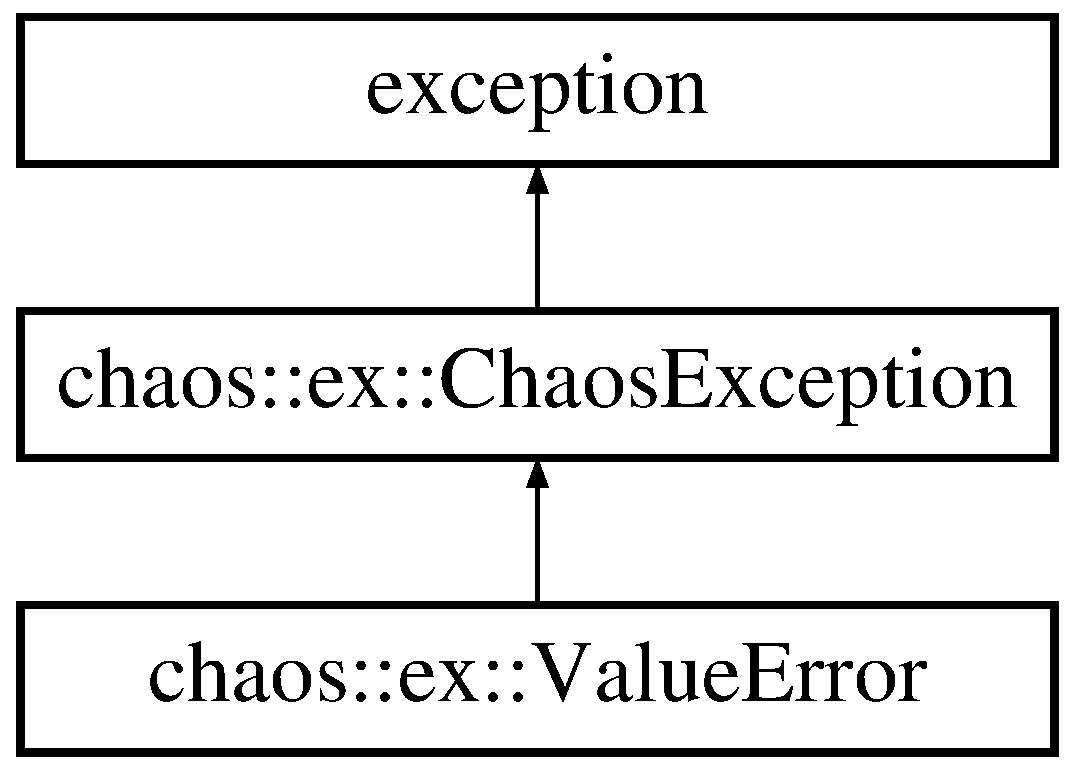
\includegraphics[height=3.000000cm]{classchaos_1_1ex_1_1_value_error}
\end{center}
\end{figure}
\subsection*{Public Member Functions}
\begin{DoxyCompactItemize}
\item 
\hypertarget{classchaos_1_1ex_1_1_value_error_ad7c90b7ae603eec76908add85d311633}{}{\bfseries Value\+Error} (const \hyperlink{classchaos_1_1str_1_1_u_t_f8_string}{chaos\+::str\+::\+U\+T\+F8\+String} \&message)\label{classchaos_1_1ex_1_1_value_error_ad7c90b7ae603eec76908add85d311633}

\end{DoxyCompactItemize}
\subsection*{Additional Inherited Members}


\subsection{Detailed Description}
Warns that an invalid value has been supplied. 

The documentation for this class was generated from the following file\+:\begin{DoxyCompactItemize}
\item 
D\+:/\+Dropbox/\+Development/\+Chaos\+Core/\+Chaos\+Core/src/cxx/chaoscore/base/\hyperlink{_base_exceptions_8hpp}{Base\+Exceptions.\+hpp}\end{DoxyCompactItemize}

\hypertarget{classchaos_1_1gfx_1_1_vector2}{\section{chaos\-:\-:gfx\-:\-:Vector2 Class Reference}
\label{classchaos_1_1gfx_1_1_vector2}\index{chaos\-::gfx\-::\-Vector2@{chaos\-::gfx\-::\-Vector2}}
}


Represents a 2 dimensional vector.  




{\ttfamily \#include $<$Vector2.\-hpp$>$}

\subsection*{Public Member Functions}
\begin{DoxyCompactItemize}
\item 
\hyperlink{classchaos_1_1gfx_1_1_vector2_a9803cd26cb4f18bd3bc0f646af5bc35e}{Vector2} ()
\begin{DoxyCompactList}\small\item\em Default constructor. \end{DoxyCompactList}\item 
\hyperlink{classchaos_1_1gfx_1_1_vector2_ac01190ae1b84237183e213db95fd0606}{Vector2} (float \hyperlink{classchaos_1_1gfx_1_1_vector2_a98989a2809ad9c6ac3091550ad5f5118}{x}, float \hyperlink{classchaos_1_1gfx_1_1_vector2_adf4d8ed8e49c84c2fe1596c2b9d55d49}{y})
\begin{DoxyCompactList}\small\item\em Component constructor. \end{DoxyCompactList}\end{DoxyCompactItemize}
\subsection*{Public Attributes}
\begin{DoxyCompactItemize}
\item 
\hypertarget{classchaos_1_1gfx_1_1_vector2_a98989a2809ad9c6ac3091550ad5f5118}{float \hyperlink{classchaos_1_1gfx_1_1_vector2_a98989a2809ad9c6ac3091550ad5f5118}{x}}\label{classchaos_1_1gfx_1_1_vector2_a98989a2809ad9c6ac3091550ad5f5118}

\begin{DoxyCompactList}\small\item\em X access component of this vector. \end{DoxyCompactList}\item 
\hypertarget{classchaos_1_1gfx_1_1_vector2_adf4d8ed8e49c84c2fe1596c2b9d55d49}{float \hyperlink{classchaos_1_1gfx_1_1_vector2_adf4d8ed8e49c84c2fe1596c2b9d55d49}{y}}\label{classchaos_1_1gfx_1_1_vector2_adf4d8ed8e49c84c2fe1596c2b9d55d49}

\begin{DoxyCompactList}\small\item\em Y access component of this vector. \end{DoxyCompactList}\end{DoxyCompactItemize}


\subsection{Detailed Description}
Represents a 2 dimensional vector. 

\subsection{Constructor \& Destructor Documentation}
\hypertarget{classchaos_1_1gfx_1_1_vector2_a9803cd26cb4f18bd3bc0f646af5bc35e}{\index{chaos\-::gfx\-::\-Vector2@{chaos\-::gfx\-::\-Vector2}!Vector2@{Vector2}}
\index{Vector2@{Vector2}!chaos::gfx::Vector2@{chaos\-::gfx\-::\-Vector2}}
\subsubsection[{Vector2}]{\setlength{\rightskip}{0pt plus 5cm}chaos\-::gfx\-::\-Vector2\-::\-Vector2 (
\begin{DoxyParamCaption}
{}
\end{DoxyParamCaption}
)}}\label{classchaos_1_1gfx_1_1_vector2_a9803cd26cb4f18bd3bc0f646af5bc35e}


Default constructor. 

Creates a new \hyperlink{classchaos_1_1gfx_1_1_vector2}{Vector2} with the x and y components initialised as 0. \hypertarget{classchaos_1_1gfx_1_1_vector2_ac01190ae1b84237183e213db95fd0606}{\index{chaos\-::gfx\-::\-Vector2@{chaos\-::gfx\-::\-Vector2}!Vector2@{Vector2}}
\index{Vector2@{Vector2}!chaos::gfx::Vector2@{chaos\-::gfx\-::\-Vector2}}
\subsubsection[{Vector2}]{\setlength{\rightskip}{0pt plus 5cm}chaos\-::gfx\-::\-Vector2\-::\-Vector2 (
\begin{DoxyParamCaption}
\item[{float}]{x, }
\item[{float}]{y}
\end{DoxyParamCaption}
)}}\label{classchaos_1_1gfx_1_1_vector2_ac01190ae1b84237183e213db95fd0606}


Component constructor. 

Creates a new \hyperlink{classchaos_1_1gfx_1_1_vector2}{Vector2} with the given x any y component values. 

The documentation for this class was generated from the following file\-:\begin{DoxyCompactItemize}
\item 
/home/david/\-Dropbox/\-Development/\-Chaos\-Core/\-Chaos\-Core/src/cxx/chaoscore/gfx/Vector2.\-hpp\end{DoxyCompactItemize}

\hypertarget{classchaos_1_1gfx_1_1_vector3}{\section{chaos\-:\-:gfx\-:\-:Vector3 Class Reference}
\label{classchaos_1_1gfx_1_1_vector3}\index{chaos\-::gfx\-::\-Vector3@{chaos\-::gfx\-::\-Vector3}}
}


Represents a 3 dimensional vector.  




{\ttfamily \#include $<$Vector3.\-hpp$>$}

\subsection*{Public Member Functions}
\begin{DoxyCompactItemize}
\item 
\hyperlink{classchaos_1_1gfx_1_1_vector3_a8cd3092f89afc127d6fd993e3291bd2b}{Vector3} ()
\begin{DoxyCompactList}\small\item\em Default constructor. \end{DoxyCompactList}\item 
\hyperlink{classchaos_1_1gfx_1_1_vector3_a62a4131e3f8bfbc1fc076149db944c94}{Vector3} (float \hyperlink{classchaos_1_1gfx_1_1_vector3_ac58f0d4a6e611ae3eec8e9f56476fc13}{x}, float \hyperlink{classchaos_1_1gfx_1_1_vector3_ac001a2e7468d6c6cfc5119d486817f0b}{y}, float \hyperlink{classchaos_1_1gfx_1_1_vector3_a7ec457e7ef3054557dacdc89bf7ce77b}{z})
\begin{DoxyCompactList}\small\item\em Component constructor. \end{DoxyCompactList}\item 
\hyperlink{classchaos_1_1gfx_1_1_vector3_a0ab061f754dac90c843317d979defb70}{Vector3} (float scalar)
\begin{DoxyCompactList}\small\item\em Scalar constructor. \end{DoxyCompactList}\item 
\hyperlink{classchaos_1_1gfx_1_1_vector3_a32fd7944a73e7f8d9bb6a9e6ee6d4bce}{Vector3} (const \hyperlink{classchaos_1_1gfx_1_1_vector3}{Vector3} \&other)
\begin{DoxyCompactList}\small\item\em Copy constructor. \end{DoxyCompactList}\item 
\hyperlink{classchaos_1_1gfx_1_1_vector3}{Vector3} \& \hyperlink{classchaos_1_1gfx_1_1_vector3_a3c26200a523e201ef3697797732951cb}{operator=} (const \hyperlink{classchaos_1_1gfx_1_1_vector3}{Vector3} \&other)
\begin{DoxyCompactList}\small\item\em Assignment operator. \end{DoxyCompactList}\item 
bool \hyperlink{classchaos_1_1gfx_1_1_vector3_aea8b9895ae2781f79a02dde0e22a1938}{operator==} (const \hyperlink{classchaos_1_1gfx_1_1_vector3}{Vector3} \&other) const 
\begin{DoxyCompactList}\small\item\em Equality operator. \end{DoxyCompactList}\item 
bool \hyperlink{classchaos_1_1gfx_1_1_vector3_ad8ceb4ba622ba969ab58f163d32f8e6e}{operator!=} (const \hyperlink{classchaos_1_1gfx_1_1_vector3}{Vector3} \&other) const 
\begin{DoxyCompactList}\small\item\em Inequality operator. \end{DoxyCompactList}\item 
\hyperlink{classchaos_1_1gfx_1_1_vector3}{Vector3} \hyperlink{classchaos_1_1gfx_1_1_vector3_a70135c109acc45256567d9c50f160bda}{operator+} (float scalar) const 
\begin{DoxyCompactList}\small\item\em Scalar addition operator. \end{DoxyCompactList}\item 
\hyperlink{classchaos_1_1gfx_1_1_vector3}{Vector3} \& \hyperlink{classchaos_1_1gfx_1_1_vector3_acb76c6c076cc7448503b09edab578569}{operator+=} (float scalar)
\begin{DoxyCompactList}\small\item\em Scalar compound addition operator. \end{DoxyCompactList}\item 
\hyperlink{classchaos_1_1gfx_1_1_vector3}{Vector3} \hyperlink{classchaos_1_1gfx_1_1_vector3_a94c67b5eb0b4bba1732019bc9eef459f}{operator+} (const \hyperlink{classchaos_1_1gfx_1_1_vector3}{Vector3} \&other) const 
\begin{DoxyCompactList}\small\item\em Vector addition operator. \end{DoxyCompactList}\item 
\hyperlink{classchaos_1_1gfx_1_1_vector3}{Vector3} \& \hyperlink{classchaos_1_1gfx_1_1_vector3_a05bb1715123edd7d137ebe2277d0b16f}{operator+=} (const \hyperlink{classchaos_1_1gfx_1_1_vector3}{Vector3} \&other)
\begin{DoxyCompactList}\small\item\em Vector compound addition operator. \end{DoxyCompactList}\item 
\hyperlink{classchaos_1_1gfx_1_1_vector3}{Vector3} \hyperlink{classchaos_1_1gfx_1_1_vector3_a4dae54ff2ff65a8a43572e7aad2b21ba}{operator-\/} (float scalar) const 
\begin{DoxyCompactList}\small\item\em Scalar subtraction operator. \end{DoxyCompactList}\item 
\hyperlink{classchaos_1_1gfx_1_1_vector3}{Vector3} \& \hyperlink{classchaos_1_1gfx_1_1_vector3_a7da527567f0c3f950386cfde14e0c01a}{operator-\/=} (float scalar)
\begin{DoxyCompactList}\small\item\em Scalar compound subtraction operator. \end{DoxyCompactList}\item 
\hyperlink{classchaos_1_1gfx_1_1_vector3}{Vector3} \hyperlink{classchaos_1_1gfx_1_1_vector3_aa04a47959b61f1e3f1c48b8709889f9d}{operator-\/} (const \hyperlink{classchaos_1_1gfx_1_1_vector3}{Vector3} \&other) const 
\begin{DoxyCompactList}\small\item\em Vector subtraction operator. \end{DoxyCompactList}\item 
\hyperlink{classchaos_1_1gfx_1_1_vector3}{Vector3} \& \hyperlink{classchaos_1_1gfx_1_1_vector3_a66c22970fa9dc7499b894313d1c66961}{operator-\/=} (const \hyperlink{classchaos_1_1gfx_1_1_vector3}{Vector3} \&other)
\begin{DoxyCompactList}\small\item\em Vector compound subtraction operator. \end{DoxyCompactList}\item 
\hyperlink{classchaos_1_1gfx_1_1_vector3}{Vector3} \hyperlink{classchaos_1_1gfx_1_1_vector3_a39855071d6101e932fe6fb382e3a2f9e}{operator$\ast$} (float scalar) const 
\begin{DoxyCompactList}\small\item\em Scalar multiplication operator. \end{DoxyCompactList}\item 
\hyperlink{classchaos_1_1gfx_1_1_vector3}{Vector3} \& \hyperlink{classchaos_1_1gfx_1_1_vector3_abd751363ea77af4f9e673cf092f49473}{operator$\ast$=} (float scalar)
\begin{DoxyCompactList}\small\item\em Scalar compound multiplication operator. \end{DoxyCompactList}\item 
\hyperlink{classchaos_1_1gfx_1_1_vector3}{Vector3} \hyperlink{classchaos_1_1gfx_1_1_vector3_abc909457ea9721592932f00502978886}{operator/} (float scalar) const 
\begin{DoxyCompactList}\small\item\em Scalar division operator. \end{DoxyCompactList}\item 
\hyperlink{classchaos_1_1gfx_1_1_vector3}{Vector3} \& \hyperlink{classchaos_1_1gfx_1_1_vector3_a9f61bd9beaabb1de857258d96d46c093}{operator/=} (float scalar)
\begin{DoxyCompactList}\small\item\em Scalar compound division operator. \end{DoxyCompactList}\end{DoxyCompactItemize}
\subsection*{Public Attributes}
\begin{DoxyCompactItemize}
\item 
\hypertarget{classchaos_1_1gfx_1_1_vector3_ac58f0d4a6e611ae3eec8e9f56476fc13}{float \hyperlink{classchaos_1_1gfx_1_1_vector3_ac58f0d4a6e611ae3eec8e9f56476fc13}{x}}\label{classchaos_1_1gfx_1_1_vector3_ac58f0d4a6e611ae3eec8e9f56476fc13}

\begin{DoxyCompactList}\small\item\em X component of this \hyperlink{classchaos_1_1gfx_1_1_vector3}{Vector3}. \end{DoxyCompactList}\item 
\hypertarget{classchaos_1_1gfx_1_1_vector3_ac001a2e7468d6c6cfc5119d486817f0b}{float \hyperlink{classchaos_1_1gfx_1_1_vector3_ac001a2e7468d6c6cfc5119d486817f0b}{y}}\label{classchaos_1_1gfx_1_1_vector3_ac001a2e7468d6c6cfc5119d486817f0b}

\begin{DoxyCompactList}\small\item\em Y component of this \hyperlink{classchaos_1_1gfx_1_1_vector3}{Vector3}. \end{DoxyCompactList}\item 
\hypertarget{classchaos_1_1gfx_1_1_vector3_a7ec457e7ef3054557dacdc89bf7ce77b}{float \hyperlink{classchaos_1_1gfx_1_1_vector3_a7ec457e7ef3054557dacdc89bf7ce77b}{z}}\label{classchaos_1_1gfx_1_1_vector3_a7ec457e7ef3054557dacdc89bf7ce77b}

\begin{DoxyCompactList}\small\item\em Z component of this \hyperlink{classchaos_1_1gfx_1_1_vector3}{Vector3}. \end{DoxyCompactList}\end{DoxyCompactItemize}


\subsection{Detailed Description}
Represents a 3 dimensional vector. 

\subsection{Constructor \& Destructor Documentation}
\hypertarget{classchaos_1_1gfx_1_1_vector3_a8cd3092f89afc127d6fd993e3291bd2b}{\index{chaos\-::gfx\-::\-Vector3@{chaos\-::gfx\-::\-Vector3}!Vector3@{Vector3}}
\index{Vector3@{Vector3}!chaos::gfx::Vector3@{chaos\-::gfx\-::\-Vector3}}
\subsubsection[{Vector3}]{\setlength{\rightskip}{0pt plus 5cm}chaos\-::gfx\-::\-Vector3\-::\-Vector3 (
\begin{DoxyParamCaption}
{}
\end{DoxyParamCaption}
)}}\label{classchaos_1_1gfx_1_1_vector3_a8cd3092f89afc127d6fd993e3291bd2b}


Default constructor. 

Creates a new \hyperlink{classchaos_1_1gfx_1_1_vector3}{Vector3} with the x, y, and z components initialized as 0. \hypertarget{classchaos_1_1gfx_1_1_vector3_a62a4131e3f8bfbc1fc076149db944c94}{\index{chaos\-::gfx\-::\-Vector3@{chaos\-::gfx\-::\-Vector3}!Vector3@{Vector3}}
\index{Vector3@{Vector3}!chaos::gfx::Vector3@{chaos\-::gfx\-::\-Vector3}}
\subsubsection[{Vector3}]{\setlength{\rightskip}{0pt plus 5cm}chaos\-::gfx\-::\-Vector3\-::\-Vector3 (
\begin{DoxyParamCaption}
\item[{float}]{x, }
\item[{float}]{y, }
\item[{float}]{z}
\end{DoxyParamCaption}
)}}\label{classchaos_1_1gfx_1_1_vector3_a62a4131e3f8bfbc1fc076149db944c94}


Component constructor. 

Creates a new \hyperlink{classchaos_1_1gfx_1_1_vector3}{Vector3} with the given x, y, and z component values. \hypertarget{classchaos_1_1gfx_1_1_vector3_a0ab061f754dac90c843317d979defb70}{\index{chaos\-::gfx\-::\-Vector3@{chaos\-::gfx\-::\-Vector3}!Vector3@{Vector3}}
\index{Vector3@{Vector3}!chaos::gfx::Vector3@{chaos\-::gfx\-::\-Vector3}}
\subsubsection[{Vector3}]{\setlength{\rightskip}{0pt plus 5cm}chaos\-::gfx\-::\-Vector3\-::\-Vector3 (
\begin{DoxyParamCaption}
\item[{float}]{scalar}
\end{DoxyParamCaption}
)}}\label{classchaos_1_1gfx_1_1_vector3_a0ab061f754dac90c843317d979defb70}


Scalar constructor. 

Creates a new \hyperlink{classchaos_1_1gfx_1_1_vector3}{Vector3} with the x, y, and z components initialised to the given scalar. \hypertarget{classchaos_1_1gfx_1_1_vector3_a32fd7944a73e7f8d9bb6a9e6ee6d4bce}{\index{chaos\-::gfx\-::\-Vector3@{chaos\-::gfx\-::\-Vector3}!Vector3@{Vector3}}
\index{Vector3@{Vector3}!chaos::gfx::Vector3@{chaos\-::gfx\-::\-Vector3}}
\subsubsection[{Vector3}]{\setlength{\rightskip}{0pt plus 5cm}chaos\-::gfx\-::\-Vector3\-::\-Vector3 (
\begin{DoxyParamCaption}
\item[{const {\bf Vector3} \&}]{other}
\end{DoxyParamCaption}
)}}\label{classchaos_1_1gfx_1_1_vector3_a32fd7944a73e7f8d9bb6a9e6ee6d4bce}


Copy constructor. 

Creates a new copy of the given \hyperlink{classchaos_1_1gfx_1_1_vector3}{Vector3}. 

\subsection{Member Function Documentation}
\hypertarget{classchaos_1_1gfx_1_1_vector3_a3c26200a523e201ef3697797732951cb}{\index{chaos\-::gfx\-::\-Vector3@{chaos\-::gfx\-::\-Vector3}!operator=@{operator=}}
\index{operator=@{operator=}!chaos::gfx::Vector3@{chaos\-::gfx\-::\-Vector3}}
\subsubsection[{operator=}]{\setlength{\rightskip}{0pt plus 5cm}{\bf Vector3}\& chaos\-::gfx\-::\-Vector3\-::operator= (
\begin{DoxyParamCaption}
\item[{const {\bf Vector3} \&}]{other}
\end{DoxyParamCaption}
)}}\label{classchaos_1_1gfx_1_1_vector3_a3c26200a523e201ef3697797732951cb}


Assignment operator. 

Assigns the values of this \hyperlink{classchaos_1_1gfx_1_1_vector3}{Vector3} to be a copy of the values of the other given \hyperlink{classchaos_1_1gfx_1_1_vector3}{Vector3}.


\begin{DoxyParams}{Parameters}
{\em other} & \hyperlink{classchaos_1_1gfx_1_1_vector3}{Vector3} to copy data from. \\
\hline
\end{DoxyParams}
\begin{DoxyReturn}{Returns}
A reference to this \hyperlink{classchaos_1_1gfx_1_1_vector3}{Vector3} once the assignment has taken place. 
\end{DoxyReturn}
\hypertarget{classchaos_1_1gfx_1_1_vector3_aea8b9895ae2781f79a02dde0e22a1938}{\index{chaos\-::gfx\-::\-Vector3@{chaos\-::gfx\-::\-Vector3}!operator==@{operator==}}
\index{operator==@{operator==}!chaos::gfx::Vector3@{chaos\-::gfx\-::\-Vector3}}
\subsubsection[{operator==}]{\setlength{\rightskip}{0pt plus 5cm}bool chaos\-::gfx\-::\-Vector3\-::operator== (
\begin{DoxyParamCaption}
\item[{const {\bf Vector3} \&}]{other}
\end{DoxyParamCaption}
) const}}\label{classchaos_1_1gfx_1_1_vector3_aea8b9895ae2781f79a02dde0e22a1938}


Equality operator. 

Compares whether this \hyperlink{classchaos_1_1gfx_1_1_vector3}{Vector3} and the other given \hyperlink{classchaos_1_1gfx_1_1_vector3}{Vector3} are considered \char`\"{}equal\char`\"{}. A comparison of the components of the vector is performed using \hyperlink{namespacechaos_1_1math_a45b789648ddacd3e1d2403834c1953a6}{chaos\-::math\-::float\-\_\-equals} using he default values for {\ttfamily delta\-\_\-threshold} and {\ttfamily ulps\-\_\-threshold}.


\begin{DoxyParams}{Parameters}
{\em other} & \hyperlink{classchaos_1_1gfx_1_1_vector3}{Vector3} to compare this vector against. \\
\hline
\end{DoxyParams}
\begin{DoxyReturn}{Returns}
Whether the vectors are considered equal. 
\end{DoxyReturn}
\hypertarget{classchaos_1_1gfx_1_1_vector3_ad8ceb4ba622ba969ab58f163d32f8e6e}{\index{chaos\-::gfx\-::\-Vector3@{chaos\-::gfx\-::\-Vector3}!operator!=@{operator!=}}
\index{operator!=@{operator!=}!chaos::gfx::Vector3@{chaos\-::gfx\-::\-Vector3}}
\subsubsection[{operator!=}]{\setlength{\rightskip}{0pt plus 5cm}bool chaos\-::gfx\-::\-Vector3\-::operator!= (
\begin{DoxyParamCaption}
\item[{const {\bf Vector3} \&}]{other}
\end{DoxyParamCaption}
) const}}\label{classchaos_1_1gfx_1_1_vector3_ad8ceb4ba622ba969ab58f163d32f8e6e}


Inequality operator. 

Compares this \hyperlink{classchaos_1_1gfx_1_1_vector3}{Vector3} and the other given \hyperlink{classchaos_1_1gfx_1_1_vector3}{Vector3} are not considered \char`\"{}equal\char`\"{}. See \hyperlink{classchaos_1_1gfx_1_1_vector3_aea8b9895ae2781f79a02dde0e22a1938}{Vector3\-::operator==} for further information.


\begin{DoxyParams}{Parameters}
{\em other} & \hyperlink{classchaos_1_1gfx_1_1_vector3}{Vector3} to compare this vector against. \\
\hline
\end{DoxyParams}
\begin{DoxyReturn}{Returns}
Whether the vectors are not considered equal. 
\end{DoxyReturn}
\hypertarget{classchaos_1_1gfx_1_1_vector3_a70135c109acc45256567d9c50f160bda}{\index{chaos\-::gfx\-::\-Vector3@{chaos\-::gfx\-::\-Vector3}!operator+@{operator+}}
\index{operator+@{operator+}!chaos::gfx::Vector3@{chaos\-::gfx\-::\-Vector3}}
\subsubsection[{operator+}]{\setlength{\rightskip}{0pt plus 5cm}{\bf Vector3} chaos\-::gfx\-::\-Vector3\-::operator+ (
\begin{DoxyParamCaption}
\item[{float}]{scalar}
\end{DoxyParamCaption}
) const}}\label{classchaos_1_1gfx_1_1_vector3_a70135c109acc45256567d9c50f160bda}


Scalar addition operator. 


\begin{DoxyParams}{Parameters}
{\em scalar} & The scalar to add to this \hyperlink{classchaos_1_1gfx_1_1_vector3}{Vector3}. \\
\hline
\end{DoxyParams}
\begin{DoxyReturn}{Returns}
A new \hyperlink{classchaos_1_1gfx_1_1_vector3}{Vector3} containing the results of the addition. 
\end{DoxyReturn}
\hypertarget{classchaos_1_1gfx_1_1_vector3_acb76c6c076cc7448503b09edab578569}{\index{chaos\-::gfx\-::\-Vector3@{chaos\-::gfx\-::\-Vector3}!operator+=@{operator+=}}
\index{operator+=@{operator+=}!chaos::gfx::Vector3@{chaos\-::gfx\-::\-Vector3}}
\subsubsection[{operator+=}]{\setlength{\rightskip}{0pt plus 5cm}{\bf Vector3}\& chaos\-::gfx\-::\-Vector3\-::operator+= (
\begin{DoxyParamCaption}
\item[{float}]{scalar}
\end{DoxyParamCaption}
)}}\label{classchaos_1_1gfx_1_1_vector3_acb76c6c076cc7448503b09edab578569}


Scalar compound addition operator. 


\begin{DoxyParams}{Parameters}
{\em scalar} & The scalar to add to this \hyperlink{classchaos_1_1gfx_1_1_vector3}{Vector3}. \\
\hline
\end{DoxyParams}
\begin{DoxyReturn}{Returns}
A reference to this \hyperlink{classchaos_1_1gfx_1_1_vector3}{Vector3} once the addition has taken place. 
\end{DoxyReturn}
\hypertarget{classchaos_1_1gfx_1_1_vector3_a94c67b5eb0b4bba1732019bc9eef459f}{\index{chaos\-::gfx\-::\-Vector3@{chaos\-::gfx\-::\-Vector3}!operator+@{operator+}}
\index{operator+@{operator+}!chaos::gfx::Vector3@{chaos\-::gfx\-::\-Vector3}}
\subsubsection[{operator+}]{\setlength{\rightskip}{0pt plus 5cm}{\bf Vector3} chaos\-::gfx\-::\-Vector3\-::operator+ (
\begin{DoxyParamCaption}
\item[{const {\bf Vector3} \&}]{other}
\end{DoxyParamCaption}
) const}}\label{classchaos_1_1gfx_1_1_vector3_a94c67b5eb0b4bba1732019bc9eef459f}


Vector addition operator. 


\begin{DoxyParams}{Parameters}
{\em other} & The other \hyperlink{classchaos_1_1gfx_1_1_vector3}{Vector3} to add to this \hyperlink{classchaos_1_1gfx_1_1_vector3}{Vector3} \\
\hline
\end{DoxyParams}
\begin{DoxyReturn}{Returns}
A new \hyperlink{classchaos_1_1gfx_1_1_vector3}{Vector3} containing the results of the addition. 
\end{DoxyReturn}
\hypertarget{classchaos_1_1gfx_1_1_vector3_a05bb1715123edd7d137ebe2277d0b16f}{\index{chaos\-::gfx\-::\-Vector3@{chaos\-::gfx\-::\-Vector3}!operator+=@{operator+=}}
\index{operator+=@{operator+=}!chaos::gfx::Vector3@{chaos\-::gfx\-::\-Vector3}}
\subsubsection[{operator+=}]{\setlength{\rightskip}{0pt plus 5cm}{\bf Vector3}\& chaos\-::gfx\-::\-Vector3\-::operator+= (
\begin{DoxyParamCaption}
\item[{const {\bf Vector3} \&}]{other}
\end{DoxyParamCaption}
)}}\label{classchaos_1_1gfx_1_1_vector3_a05bb1715123edd7d137ebe2277d0b16f}


Vector compound addition operator. 


\begin{DoxyParams}{Parameters}
{\em other} & The other \hyperlink{classchaos_1_1gfx_1_1_vector3}{Vector3} to add to this \hyperlink{classchaos_1_1gfx_1_1_vector3}{Vector3}. \\
\hline
\end{DoxyParams}
\begin{DoxyReturn}{Returns}
A reference to this \hyperlink{classchaos_1_1gfx_1_1_vector3}{Vector3} once the addition has taken place. 
\end{DoxyReturn}
\hypertarget{classchaos_1_1gfx_1_1_vector3_a4dae54ff2ff65a8a43572e7aad2b21ba}{\index{chaos\-::gfx\-::\-Vector3@{chaos\-::gfx\-::\-Vector3}!operator-\/@{operator-\/}}
\index{operator-\/@{operator-\/}!chaos::gfx::Vector3@{chaos\-::gfx\-::\-Vector3}}
\subsubsection[{operator-\/}]{\setlength{\rightskip}{0pt plus 5cm}{\bf Vector3} chaos\-::gfx\-::\-Vector3\-::operator-\/ (
\begin{DoxyParamCaption}
\item[{float}]{scalar}
\end{DoxyParamCaption}
) const}}\label{classchaos_1_1gfx_1_1_vector3_a4dae54ff2ff65a8a43572e7aad2b21ba}


Scalar subtraction operator. 


\begin{DoxyParams}{Parameters}
{\em scalar} & The scalar to subtract from this \hyperlink{classchaos_1_1gfx_1_1_vector3}{Vector3}. \\
\hline
\end{DoxyParams}
\begin{DoxyReturn}{Returns}
A new \hyperlink{classchaos_1_1gfx_1_1_vector3}{Vector3} containing the results of the subtraction. 
\end{DoxyReturn}
\hypertarget{classchaos_1_1gfx_1_1_vector3_a7da527567f0c3f950386cfde14e0c01a}{\index{chaos\-::gfx\-::\-Vector3@{chaos\-::gfx\-::\-Vector3}!operator-\/=@{operator-\/=}}
\index{operator-\/=@{operator-\/=}!chaos::gfx::Vector3@{chaos\-::gfx\-::\-Vector3}}
\subsubsection[{operator-\/=}]{\setlength{\rightskip}{0pt plus 5cm}{\bf Vector3}\& chaos\-::gfx\-::\-Vector3\-::operator-\/= (
\begin{DoxyParamCaption}
\item[{float}]{scalar}
\end{DoxyParamCaption}
)}}\label{classchaos_1_1gfx_1_1_vector3_a7da527567f0c3f950386cfde14e0c01a}


Scalar compound subtraction operator. 


\begin{DoxyParams}{Parameters}
{\em scalar} & The scalar to subtract from this \hyperlink{classchaos_1_1gfx_1_1_vector3}{Vector3}. \\
\hline
\end{DoxyParams}
\begin{DoxyReturn}{Returns}
A reference to this \hyperlink{classchaos_1_1gfx_1_1_vector3}{Vector3} once the subtraction has taken place. 
\end{DoxyReturn}
\hypertarget{classchaos_1_1gfx_1_1_vector3_aa04a47959b61f1e3f1c48b8709889f9d}{\index{chaos\-::gfx\-::\-Vector3@{chaos\-::gfx\-::\-Vector3}!operator-\/@{operator-\/}}
\index{operator-\/@{operator-\/}!chaos::gfx::Vector3@{chaos\-::gfx\-::\-Vector3}}
\subsubsection[{operator-\/}]{\setlength{\rightskip}{0pt plus 5cm}{\bf Vector3} chaos\-::gfx\-::\-Vector3\-::operator-\/ (
\begin{DoxyParamCaption}
\item[{const {\bf Vector3} \&}]{other}
\end{DoxyParamCaption}
) const}}\label{classchaos_1_1gfx_1_1_vector3_aa04a47959b61f1e3f1c48b8709889f9d}


Vector subtraction operator. 


\begin{DoxyParams}{Parameters}
{\em other} & The other \hyperlink{classchaos_1_1gfx_1_1_vector3}{Vector3} to subtract from this \hyperlink{classchaos_1_1gfx_1_1_vector3}{Vector3}. \\
\hline
\end{DoxyParams}
\begin{DoxyReturn}{Returns}
A new \hyperlink{classchaos_1_1gfx_1_1_vector3}{Vector3} containing the results of the subtraction. 
\end{DoxyReturn}
\hypertarget{classchaos_1_1gfx_1_1_vector3_a66c22970fa9dc7499b894313d1c66961}{\index{chaos\-::gfx\-::\-Vector3@{chaos\-::gfx\-::\-Vector3}!operator-\/=@{operator-\/=}}
\index{operator-\/=@{operator-\/=}!chaos::gfx::Vector3@{chaos\-::gfx\-::\-Vector3}}
\subsubsection[{operator-\/=}]{\setlength{\rightskip}{0pt plus 5cm}{\bf Vector3}\& chaos\-::gfx\-::\-Vector3\-::operator-\/= (
\begin{DoxyParamCaption}
\item[{const {\bf Vector3} \&}]{other}
\end{DoxyParamCaption}
)}}\label{classchaos_1_1gfx_1_1_vector3_a66c22970fa9dc7499b894313d1c66961}


Vector compound subtraction operator. 


\begin{DoxyParams}{Parameters}
{\em other} & The other \hyperlink{classchaos_1_1gfx_1_1_vector3}{Vector3} to subtract from this \hyperlink{classchaos_1_1gfx_1_1_vector3}{Vector3}. \\
\hline
\end{DoxyParams}
\begin{DoxyReturn}{Returns}
A reference to this \hyperlink{classchaos_1_1gfx_1_1_vector3}{Vector3} once the subtraction has taken place. 
\end{DoxyReturn}
\hypertarget{classchaos_1_1gfx_1_1_vector3_a39855071d6101e932fe6fb382e3a2f9e}{\index{chaos\-::gfx\-::\-Vector3@{chaos\-::gfx\-::\-Vector3}!operator$\ast$@{operator$\ast$}}
\index{operator$\ast$@{operator$\ast$}!chaos::gfx::Vector3@{chaos\-::gfx\-::\-Vector3}}
\subsubsection[{operator$\ast$}]{\setlength{\rightskip}{0pt plus 5cm}{\bf Vector3} chaos\-::gfx\-::\-Vector3\-::operator$\ast$ (
\begin{DoxyParamCaption}
\item[{float}]{scalar}
\end{DoxyParamCaption}
) const}}\label{classchaos_1_1gfx_1_1_vector3_a39855071d6101e932fe6fb382e3a2f9e}


Scalar multiplication operator. 


\begin{DoxyParams}{Parameters}
{\em scalar} & The scalar to multiply this \hyperlink{classchaos_1_1gfx_1_1_vector3}{Vector3} by. \\
\hline
\end{DoxyParams}
\begin{DoxyReturn}{Returns}
A new vector containing the results of the multiplication. 
\end{DoxyReturn}
\hypertarget{classchaos_1_1gfx_1_1_vector3_abd751363ea77af4f9e673cf092f49473}{\index{chaos\-::gfx\-::\-Vector3@{chaos\-::gfx\-::\-Vector3}!operator$\ast$=@{operator$\ast$=}}
\index{operator$\ast$=@{operator$\ast$=}!chaos::gfx::Vector3@{chaos\-::gfx\-::\-Vector3}}
\subsubsection[{operator$\ast$=}]{\setlength{\rightskip}{0pt plus 5cm}{\bf Vector3}\& chaos\-::gfx\-::\-Vector3\-::operator$\ast$= (
\begin{DoxyParamCaption}
\item[{float}]{scalar}
\end{DoxyParamCaption}
)}}\label{classchaos_1_1gfx_1_1_vector3_abd751363ea77af4f9e673cf092f49473}


Scalar compound multiplication operator. 


\begin{DoxyParams}{Parameters}
{\em scalar} & The scalar to multiply this \hyperlink{classchaos_1_1gfx_1_1_vector3}{Vector3} by. \\
\hline
\end{DoxyParams}
\begin{DoxyReturn}{Returns}
A reference to this \hyperlink{classchaos_1_1gfx_1_1_vector3}{Vector3} once the multiplication has taken place. 
\end{DoxyReturn}
\hypertarget{classchaos_1_1gfx_1_1_vector3_abc909457ea9721592932f00502978886}{\index{chaos\-::gfx\-::\-Vector3@{chaos\-::gfx\-::\-Vector3}!operator/@{operator/}}
\index{operator/@{operator/}!chaos::gfx::Vector3@{chaos\-::gfx\-::\-Vector3}}
\subsubsection[{operator/}]{\setlength{\rightskip}{0pt plus 5cm}{\bf Vector3} chaos\-::gfx\-::\-Vector3\-::operator/ (
\begin{DoxyParamCaption}
\item[{float}]{scalar}
\end{DoxyParamCaption}
) const}}\label{classchaos_1_1gfx_1_1_vector3_abc909457ea9721592932f00502978886}


Scalar division operator. 


\begin{DoxyParams}{Parameters}
{\em scalar} & The scalar to divide this \hyperlink{classchaos_1_1gfx_1_1_vector3}{Vector3} by. \\
\hline
\end{DoxyParams}
\begin{DoxyReturn}{Returns}
A new \hyperlink{classchaos_1_1gfx_1_1_vector3}{Vector3} containing the results of the division. 
\end{DoxyReturn}
\hypertarget{classchaos_1_1gfx_1_1_vector3_a9f61bd9beaabb1de857258d96d46c093}{\index{chaos\-::gfx\-::\-Vector3@{chaos\-::gfx\-::\-Vector3}!operator/=@{operator/=}}
\index{operator/=@{operator/=}!chaos::gfx::Vector3@{chaos\-::gfx\-::\-Vector3}}
\subsubsection[{operator/=}]{\setlength{\rightskip}{0pt plus 5cm}{\bf Vector3}\& chaos\-::gfx\-::\-Vector3\-::operator/= (
\begin{DoxyParamCaption}
\item[{float}]{scalar}
\end{DoxyParamCaption}
)}}\label{classchaos_1_1gfx_1_1_vector3_a9f61bd9beaabb1de857258d96d46c093}


Scalar compound division operator. 


\begin{DoxyParams}{Parameters}
{\em scalar} & The scalar to divide this \hyperlink{classchaos_1_1gfx_1_1_vector3}{Vector3} by. \\
\hline
\end{DoxyParams}
\begin{DoxyReturn}{Returns}
A reference to this \hyperlink{classchaos_1_1gfx_1_1_vector3}{Vector3} once the division has taken place. 
\end{DoxyReturn}


The documentation for this class was generated from the following file\-:\begin{DoxyCompactItemize}
\item 
/home/david/\-Dropbox/\-Development/\-Chaos\-Core/\-Chaos\-Core/src/cxx/chaoscore/gfx/Vector3.\-hpp\end{DoxyCompactItemize}

\hypertarget{classchaos_1_1gfx_1_1_vector4}{\section{chaos\-:\-:gfx\-:\-:Vector4 Class Reference}
\label{classchaos_1_1gfx_1_1_vector4}\index{chaos\-::gfx\-::\-Vector4@{chaos\-::gfx\-::\-Vector4}}
}
\subsection*{Public Member Functions}
\begin{DoxyCompactItemize}
\item 
\hyperlink{classchaos_1_1gfx_1_1_vector4_abdee87e0c5bbd7a9870957951f2bba80}{Vector4} ()
\begin{DoxyCompactList}\small\item\em Default constructor. \end{DoxyCompactList}\item 
\hyperlink{classchaos_1_1gfx_1_1_vector4_a8e22c6ae7ba175d15bd8804cff77519e}{Vector4} (float \hyperlink{classchaos_1_1gfx_1_1_vector4_a74f8e26ec8f6c55a11ed5a423fb0eec4}{x}, float \hyperlink{classchaos_1_1gfx_1_1_vector4_aa823679c8ce9d8b882f7e05f5670ee74}{y}, float \hyperlink{classchaos_1_1gfx_1_1_vector4_ae1e282cb0c262db6c20f29c34d727938}{z}, float \hyperlink{classchaos_1_1gfx_1_1_vector4_a3cd40a2e6ce1fd10a0d2c8136965e9dd}{w})
\begin{DoxyCompactList}\small\item\em Component constructor. \end{DoxyCompactList}\item 
\hyperlink{classchaos_1_1gfx_1_1_vector4_aa2630f2dfef3d7a9ae5b284be502f528}{Vector4} (float scalar)
\begin{DoxyCompactList}\small\item\em Scalar constructor. \end{DoxyCompactList}\item 
\hyperlink{classchaos_1_1gfx_1_1_vector4_aabd97977b6470d2e03ab15d7fe5e0678}{Vector4} (const \hyperlink{classchaos_1_1gfx_1_1_vector4}{Vector4} \&other)
\begin{DoxyCompactList}\small\item\em Copy constructor. \end{DoxyCompactList}\item 
\hyperlink{classchaos_1_1gfx_1_1_vector4}{Vector4} \& \hyperlink{classchaos_1_1gfx_1_1_vector4_ad6b4eb3482cb75173ca23edd9f352930}{operator=} (const \hyperlink{classchaos_1_1gfx_1_1_vector4}{Vector4} \&other)
\begin{DoxyCompactList}\small\item\em Assignment operator. \end{DoxyCompactList}\item 
bool \hyperlink{classchaos_1_1gfx_1_1_vector4_add5671fb46f71d2196a68e2746309463}{operator==} (const \hyperlink{classchaos_1_1gfx_1_1_vector4}{Vector4} \&other) const 
\begin{DoxyCompactList}\small\item\em Equality operator. \end{DoxyCompactList}\item 
bool \hyperlink{classchaos_1_1gfx_1_1_vector4_ae0ac2f2346e0e56523f8f263286d3954}{operator!=} (const \hyperlink{classchaos_1_1gfx_1_1_vector4}{Vector4} \&other) const 
\begin{DoxyCompactList}\small\item\em Inequality operator. \end{DoxyCompactList}\item 
\hyperlink{classchaos_1_1gfx_1_1_vector4}{Vector4} \hyperlink{classchaos_1_1gfx_1_1_vector4_a214aefd2c36fb704f6a3e9a531e9b4c4}{operator-\/} () const 
\begin{DoxyCompactList}\small\item\em Inverse operator. \end{DoxyCompactList}\item 
\hyperlink{classchaos_1_1gfx_1_1_vector4}{Vector4} \hyperlink{classchaos_1_1gfx_1_1_vector4_aaa1fe6160bb530edada4723daa4276e0}{operator+} (float scalar) const 
\begin{DoxyCompactList}\small\item\em Scalar addition operator. \end{DoxyCompactList}\item 
\hyperlink{classchaos_1_1gfx_1_1_vector4}{Vector4} \& \hyperlink{classchaos_1_1gfx_1_1_vector4_a1ee838a2da3e2595838769850a4a945f}{operator+=} (float scalar)
\begin{DoxyCompactList}\small\item\em Scalar compound addition operator. \end{DoxyCompactList}\item 
\hyperlink{classchaos_1_1gfx_1_1_vector4}{Vector4} \hyperlink{classchaos_1_1gfx_1_1_vector4_ab6631a4c686e6878d8d4212369300372}{operator+} (const \hyperlink{classchaos_1_1gfx_1_1_vector4}{Vector4} \&other) const 
\begin{DoxyCompactList}\small\item\em Vector addition operator. \end{DoxyCompactList}\item 
\hyperlink{classchaos_1_1gfx_1_1_vector4}{Vector4} \& \hyperlink{classchaos_1_1gfx_1_1_vector4_afda4d8356ac748b55f100ca9598fa6ab}{operator+=} (const \hyperlink{classchaos_1_1gfx_1_1_vector4}{Vector4} \&other)
\begin{DoxyCompactList}\small\item\em Vector compound addition operator. \end{DoxyCompactList}\item 
\hyperlink{classchaos_1_1gfx_1_1_vector4}{Vector4} \hyperlink{classchaos_1_1gfx_1_1_vector4_af4f001e9cb65320da1831cebcab8d859}{operator-\/} (float scalar) const 
\begin{DoxyCompactList}\small\item\em Scalar subtraction operator. \end{DoxyCompactList}\item 
\hyperlink{classchaos_1_1gfx_1_1_vector4}{Vector4} \& \hyperlink{classchaos_1_1gfx_1_1_vector4_a0d6a6c74179d2b8963b6c1bedd83bf5e}{operator-\/=} (float scalar)
\begin{DoxyCompactList}\small\item\em Scalar compound subtraction operator. \end{DoxyCompactList}\item 
\hyperlink{classchaos_1_1gfx_1_1_vector4}{Vector4} \hyperlink{classchaos_1_1gfx_1_1_vector4_af923be6632e670c30a3e86683b47d903}{operator-\/} (const \hyperlink{classchaos_1_1gfx_1_1_vector4}{Vector4} \&other) const 
\begin{DoxyCompactList}\small\item\em Vector subtraction operator. \end{DoxyCompactList}\item 
\hyperlink{classchaos_1_1gfx_1_1_vector4}{Vector4} \& \hyperlink{classchaos_1_1gfx_1_1_vector4_aba6caefa7d369b2019347462999802ea}{operator-\/=} (const \hyperlink{classchaos_1_1gfx_1_1_vector4}{Vector4} \&other)
\begin{DoxyCompactList}\small\item\em Vector compound subtraction operator. \end{DoxyCompactList}\item 
\hyperlink{classchaos_1_1gfx_1_1_vector4}{Vector4} \hyperlink{classchaos_1_1gfx_1_1_vector4_afee77ed144ba58fae3877ddbebcd75d3}{operator$\ast$} (float scalar) const 
\begin{DoxyCompactList}\small\item\em Scalar multiplication operator. \end{DoxyCompactList}\item 
\hyperlink{classchaos_1_1gfx_1_1_vector4}{Vector4} \& \hyperlink{classchaos_1_1gfx_1_1_vector4_ae171d478578a7a1564ca3e869da3b3f8}{operator$\ast$=} (float scalar)
\begin{DoxyCompactList}\small\item\em Scalar compound multiplication operator. \end{DoxyCompactList}\item 
\hyperlink{classchaos_1_1gfx_1_1_vector4}{Vector4} \hyperlink{classchaos_1_1gfx_1_1_vector4_accffe88c758a09b13b68ee1692663de9}{operator/} (float scalar) const 
\begin{DoxyCompactList}\small\item\em Scalar division operator. \end{DoxyCompactList}\item 
\hyperlink{classchaos_1_1gfx_1_1_vector4}{Vector4} \& \hyperlink{classchaos_1_1gfx_1_1_vector4_a1ce1c817fbc1999faeb34d08f4df284b}{operator/=} (float scalar)
\begin{DoxyCompactList}\small\item\em Scalar compound division operator. \end{DoxyCompactList}\end{DoxyCompactItemize}
\subsection*{Public Attributes}
\begin{DoxyCompactItemize}
\item 
\hypertarget{classchaos_1_1gfx_1_1_vector4_a74f8e26ec8f6c55a11ed5a423fb0eec4}{float \hyperlink{classchaos_1_1gfx_1_1_vector4_a74f8e26ec8f6c55a11ed5a423fb0eec4}{x}}\label{classchaos_1_1gfx_1_1_vector4_a74f8e26ec8f6c55a11ed5a423fb0eec4}

\begin{DoxyCompactList}\small\item\em X component of this \hyperlink{classchaos_1_1gfx_1_1_vector4}{Vector4}. \end{DoxyCompactList}\item 
\hypertarget{classchaos_1_1gfx_1_1_vector4_aa823679c8ce9d8b882f7e05f5670ee74}{float \hyperlink{classchaos_1_1gfx_1_1_vector4_aa823679c8ce9d8b882f7e05f5670ee74}{y}}\label{classchaos_1_1gfx_1_1_vector4_aa823679c8ce9d8b882f7e05f5670ee74}

\begin{DoxyCompactList}\small\item\em Y component of this \hyperlink{classchaos_1_1gfx_1_1_vector4}{Vector4}. \end{DoxyCompactList}\item 
\hypertarget{classchaos_1_1gfx_1_1_vector4_ae1e282cb0c262db6c20f29c34d727938}{float \hyperlink{classchaos_1_1gfx_1_1_vector4_ae1e282cb0c262db6c20f29c34d727938}{z}}\label{classchaos_1_1gfx_1_1_vector4_ae1e282cb0c262db6c20f29c34d727938}

\begin{DoxyCompactList}\small\item\em Z component of this \hyperlink{classchaos_1_1gfx_1_1_vector4}{Vector4}. \end{DoxyCompactList}\item 
\hypertarget{classchaos_1_1gfx_1_1_vector4_a3cd40a2e6ce1fd10a0d2c8136965e9dd}{float \hyperlink{classchaos_1_1gfx_1_1_vector4_a3cd40a2e6ce1fd10a0d2c8136965e9dd}{w}}\label{classchaos_1_1gfx_1_1_vector4_a3cd40a2e6ce1fd10a0d2c8136965e9dd}

\begin{DoxyCompactList}\small\item\em W component of this \hyperlink{classchaos_1_1gfx_1_1_vector4}{Vector4}. \end{DoxyCompactList}\end{DoxyCompactItemize}


\subsection{Constructor \& Destructor Documentation}
\hypertarget{classchaos_1_1gfx_1_1_vector4_abdee87e0c5bbd7a9870957951f2bba80}{\index{chaos\-::gfx\-::\-Vector4@{chaos\-::gfx\-::\-Vector4}!Vector4@{Vector4}}
\index{Vector4@{Vector4}!chaos::gfx::Vector4@{chaos\-::gfx\-::\-Vector4}}
\subsubsection[{Vector4}]{\setlength{\rightskip}{0pt plus 5cm}chaos\-::gfx\-::\-Vector4\-::\-Vector4 (
\begin{DoxyParamCaption}
{}
\end{DoxyParamCaption}
)}}\label{classchaos_1_1gfx_1_1_vector4_abdee87e0c5bbd7a9870957951f2bba80}


Default constructor. 

Creates a new \hyperlink{classchaos_1_1gfx_1_1_vector4}{Vector4} with the x, y, z, and w components initialised as 0. \hypertarget{classchaos_1_1gfx_1_1_vector4_a8e22c6ae7ba175d15bd8804cff77519e}{\index{chaos\-::gfx\-::\-Vector4@{chaos\-::gfx\-::\-Vector4}!Vector4@{Vector4}}
\index{Vector4@{Vector4}!chaos::gfx::Vector4@{chaos\-::gfx\-::\-Vector4}}
\subsubsection[{Vector4}]{\setlength{\rightskip}{0pt plus 5cm}chaos\-::gfx\-::\-Vector4\-::\-Vector4 (
\begin{DoxyParamCaption}
\item[{float}]{x, }
\item[{float}]{y, }
\item[{float}]{z, }
\item[{float}]{w}
\end{DoxyParamCaption}
)}}\label{classchaos_1_1gfx_1_1_vector4_a8e22c6ae7ba175d15bd8804cff77519e}


Component constructor. 

Creates a new \hyperlink{classchaos_1_1gfx_1_1_vector4}{Vector4} with the given x, y, z, and w component values. \hypertarget{classchaos_1_1gfx_1_1_vector4_aa2630f2dfef3d7a9ae5b284be502f528}{\index{chaos\-::gfx\-::\-Vector4@{chaos\-::gfx\-::\-Vector4}!Vector4@{Vector4}}
\index{Vector4@{Vector4}!chaos::gfx::Vector4@{chaos\-::gfx\-::\-Vector4}}
\subsubsection[{Vector4}]{\setlength{\rightskip}{0pt plus 5cm}chaos\-::gfx\-::\-Vector4\-::\-Vector4 (
\begin{DoxyParamCaption}
\item[{float}]{scalar}
\end{DoxyParamCaption}
)}}\label{classchaos_1_1gfx_1_1_vector4_aa2630f2dfef3d7a9ae5b284be502f528}


Scalar constructor. 

Creates a new \hyperlink{classchaos_1_1gfx_1_1_vector4}{Vector4} with the x, y, z, and w components to the given scalar. \hypertarget{classchaos_1_1gfx_1_1_vector4_aabd97977b6470d2e03ab15d7fe5e0678}{\index{chaos\-::gfx\-::\-Vector4@{chaos\-::gfx\-::\-Vector4}!Vector4@{Vector4}}
\index{Vector4@{Vector4}!chaos::gfx::Vector4@{chaos\-::gfx\-::\-Vector4}}
\subsubsection[{Vector4}]{\setlength{\rightskip}{0pt plus 5cm}chaos\-::gfx\-::\-Vector4\-::\-Vector4 (
\begin{DoxyParamCaption}
\item[{const {\bf Vector4} \&}]{other}
\end{DoxyParamCaption}
)}}\label{classchaos_1_1gfx_1_1_vector4_aabd97977b6470d2e03ab15d7fe5e0678}


Copy constructor. 

Creates a new copy of the given \hyperlink{classchaos_1_1gfx_1_1_vector4}{Vector4}. 

\subsection{Member Function Documentation}
\hypertarget{classchaos_1_1gfx_1_1_vector4_ad6b4eb3482cb75173ca23edd9f352930}{\index{chaos\-::gfx\-::\-Vector4@{chaos\-::gfx\-::\-Vector4}!operator=@{operator=}}
\index{operator=@{operator=}!chaos::gfx::Vector4@{chaos\-::gfx\-::\-Vector4}}
\subsubsection[{operator=}]{\setlength{\rightskip}{0pt plus 5cm}{\bf Vector4}\& chaos\-::gfx\-::\-Vector4\-::operator= (
\begin{DoxyParamCaption}
\item[{const {\bf Vector4} \&}]{other}
\end{DoxyParamCaption}
)}}\label{classchaos_1_1gfx_1_1_vector4_ad6b4eb3482cb75173ca23edd9f352930}


Assignment operator. 

Assigns the values of this \hyperlink{classchaos_1_1gfx_1_1_vector4}{Vector4} to be a copy of the values of the other given \hyperlink{classchaos_1_1gfx_1_1_vector4}{Vector4}.


\begin{DoxyParams}{Parameters}
{\em other} & \hyperlink{classchaos_1_1gfx_1_1_vector4}{Vector4} to copy data from. \\
\hline
\end{DoxyParams}
\begin{DoxyReturn}{Returns}
A reference to this \hyperlink{classchaos_1_1gfx_1_1_vector4}{Vector4} once the assignment has taken place. 
\end{DoxyReturn}
\hypertarget{classchaos_1_1gfx_1_1_vector4_add5671fb46f71d2196a68e2746309463}{\index{chaos\-::gfx\-::\-Vector4@{chaos\-::gfx\-::\-Vector4}!operator==@{operator==}}
\index{operator==@{operator==}!chaos::gfx::Vector4@{chaos\-::gfx\-::\-Vector4}}
\subsubsection[{operator==}]{\setlength{\rightskip}{0pt plus 5cm}bool chaos\-::gfx\-::\-Vector4\-::operator== (
\begin{DoxyParamCaption}
\item[{const {\bf Vector4} \&}]{other}
\end{DoxyParamCaption}
) const}}\label{classchaos_1_1gfx_1_1_vector4_add5671fb46f71d2196a68e2746309463}


Equality operator. 

Compares whether this \hyperlink{classchaos_1_1gfx_1_1_vector4}{Vector4} and the other given \hyperlink{classchaos_1_1gfx_1_1_vector4}{Vector4} are considered \char`\"{}equal\char`\"{}. A comparison of the component of the vector is performed using \hyperlink{namespacechaos_1_1math_a45b789648ddacd3e1d2403834c1953a6}{chaos\-::math\-::float\-\_\-equals} using the default values for {\ttfamily delta\-\_\-threshold} and {\ttfamily ulps\-\_\-threshold}.


\begin{DoxyParams}{Parameters}
{\em other} & \hyperlink{classchaos_1_1gfx_1_1_vector4}{Vector4} to compare this vector against. \\
\hline
\end{DoxyParams}
\begin{DoxyReturn}{Returns}
Whether the vectors are considered equal. 
\end{DoxyReturn}
\hypertarget{classchaos_1_1gfx_1_1_vector4_ae0ac2f2346e0e56523f8f263286d3954}{\index{chaos\-::gfx\-::\-Vector4@{chaos\-::gfx\-::\-Vector4}!operator!=@{operator!=}}
\index{operator!=@{operator!=}!chaos::gfx::Vector4@{chaos\-::gfx\-::\-Vector4}}
\subsubsection[{operator!=}]{\setlength{\rightskip}{0pt plus 5cm}bool chaos\-::gfx\-::\-Vector4\-::operator!= (
\begin{DoxyParamCaption}
\item[{const {\bf Vector4} \&}]{other}
\end{DoxyParamCaption}
) const}}\label{classchaos_1_1gfx_1_1_vector4_ae0ac2f2346e0e56523f8f263286d3954}


Inequality operator. 

Compares this \hyperlink{classchaos_1_1gfx_1_1_vector4}{Vector4} and the other given \hyperlink{classchaos_1_1gfx_1_1_vector4}{Vector4} are not considered \char`\"{}equal\char`\"{}. See \hyperlink{classchaos_1_1gfx_1_1_vector4_add5671fb46f71d2196a68e2746309463}{Vector4\-::operator==} for further information.


\begin{DoxyParams}{Parameters}
{\em other} & \hyperlink{classchaos_1_1gfx_1_1_vector4}{Vector4} to compare this vector against. \\
\hline
\end{DoxyParams}
\begin{DoxyReturn}{Returns}
Whether the vectors are not considered equal. 
\end{DoxyReturn}
\hypertarget{classchaos_1_1gfx_1_1_vector4_a214aefd2c36fb704f6a3e9a531e9b4c4}{\index{chaos\-::gfx\-::\-Vector4@{chaos\-::gfx\-::\-Vector4}!operator-\/@{operator-\/}}
\index{operator-\/@{operator-\/}!chaos::gfx::Vector4@{chaos\-::gfx\-::\-Vector4}}
\subsubsection[{operator-\/}]{\setlength{\rightskip}{0pt plus 5cm}{\bf Vector4} chaos\-::gfx\-::\-Vector4\-::operator-\/ (
\begin{DoxyParamCaption}
{}
\end{DoxyParamCaption}
) const}}\label{classchaos_1_1gfx_1_1_vector4_a214aefd2c36fb704f6a3e9a531e9b4c4}


Inverse operator. 

\begin{DoxyReturn}{Returns}
A new \hyperlink{classchaos_1_1gfx_1_1_vector4}{Vector4} which is a copy of this \hyperlink{classchaos_1_1gfx_1_1_vector4}{Vector4} with its values inverted. 
\end{DoxyReturn}
\hypertarget{classchaos_1_1gfx_1_1_vector4_aaa1fe6160bb530edada4723daa4276e0}{\index{chaos\-::gfx\-::\-Vector4@{chaos\-::gfx\-::\-Vector4}!operator+@{operator+}}
\index{operator+@{operator+}!chaos::gfx::Vector4@{chaos\-::gfx\-::\-Vector4}}
\subsubsection[{operator+}]{\setlength{\rightskip}{0pt plus 5cm}{\bf Vector4} chaos\-::gfx\-::\-Vector4\-::operator+ (
\begin{DoxyParamCaption}
\item[{float}]{scalar}
\end{DoxyParamCaption}
) const}}\label{classchaos_1_1gfx_1_1_vector4_aaa1fe6160bb530edada4723daa4276e0}


Scalar addition operator. 


\begin{DoxyParams}{Parameters}
{\em scalar} & The scalar to add to this \hyperlink{classchaos_1_1gfx_1_1_vector4}{Vector4}. \\
\hline
\end{DoxyParams}
\begin{DoxyReturn}{Returns}
A new \hyperlink{classchaos_1_1gfx_1_1_vector4}{Vector4} containing the results of the addition. 
\end{DoxyReturn}
\hypertarget{classchaos_1_1gfx_1_1_vector4_a1ee838a2da3e2595838769850a4a945f}{\index{chaos\-::gfx\-::\-Vector4@{chaos\-::gfx\-::\-Vector4}!operator+=@{operator+=}}
\index{operator+=@{operator+=}!chaos::gfx::Vector4@{chaos\-::gfx\-::\-Vector4}}
\subsubsection[{operator+=}]{\setlength{\rightskip}{0pt plus 5cm}{\bf Vector4}\& chaos\-::gfx\-::\-Vector4\-::operator+= (
\begin{DoxyParamCaption}
\item[{float}]{scalar}
\end{DoxyParamCaption}
)}}\label{classchaos_1_1gfx_1_1_vector4_a1ee838a2da3e2595838769850a4a945f}


Scalar compound addition operator. 


\begin{DoxyParams}{Parameters}
{\em scalar} & The scalar to add to this \hyperlink{classchaos_1_1gfx_1_1_vector4}{Vector4}. \\
\hline
\end{DoxyParams}
\begin{DoxyReturn}{Returns}
A reference to this \hyperlink{classchaos_1_1gfx_1_1_vector4}{Vector4} once the addition has taken place. 
\end{DoxyReturn}
\hypertarget{classchaos_1_1gfx_1_1_vector4_ab6631a4c686e6878d8d4212369300372}{\index{chaos\-::gfx\-::\-Vector4@{chaos\-::gfx\-::\-Vector4}!operator+@{operator+}}
\index{operator+@{operator+}!chaos::gfx::Vector4@{chaos\-::gfx\-::\-Vector4}}
\subsubsection[{operator+}]{\setlength{\rightskip}{0pt plus 5cm}{\bf Vector4} chaos\-::gfx\-::\-Vector4\-::operator+ (
\begin{DoxyParamCaption}
\item[{const {\bf Vector4} \&}]{other}
\end{DoxyParamCaption}
) const}}\label{classchaos_1_1gfx_1_1_vector4_ab6631a4c686e6878d8d4212369300372}


Vector addition operator. 


\begin{DoxyParams}{Parameters}
{\em other} & The other \hyperlink{classchaos_1_1gfx_1_1_vector4}{Vector4} to add to this \hyperlink{classchaos_1_1gfx_1_1_vector4}{Vector4} \\
\hline
\end{DoxyParams}
\begin{DoxyReturn}{Returns}
A new \hyperlink{classchaos_1_1gfx_1_1_vector4}{Vector4} containing the results of the addition. 
\end{DoxyReturn}
\hypertarget{classchaos_1_1gfx_1_1_vector4_afda4d8356ac748b55f100ca9598fa6ab}{\index{chaos\-::gfx\-::\-Vector4@{chaos\-::gfx\-::\-Vector4}!operator+=@{operator+=}}
\index{operator+=@{operator+=}!chaos::gfx::Vector4@{chaos\-::gfx\-::\-Vector4}}
\subsubsection[{operator+=}]{\setlength{\rightskip}{0pt plus 5cm}{\bf Vector4}\& chaos\-::gfx\-::\-Vector4\-::operator+= (
\begin{DoxyParamCaption}
\item[{const {\bf Vector4} \&}]{other}
\end{DoxyParamCaption}
)}}\label{classchaos_1_1gfx_1_1_vector4_afda4d8356ac748b55f100ca9598fa6ab}


Vector compound addition operator. 


\begin{DoxyParams}{Parameters}
{\em other} & The other \hyperlink{classchaos_1_1gfx_1_1_vector4}{Vector4} to add to this \hyperlink{classchaos_1_1gfx_1_1_vector4}{Vector4}. \\
\hline
\end{DoxyParams}
\begin{DoxyReturn}{Returns}
A reference to this \hyperlink{classchaos_1_1gfx_1_1_vector4}{Vector4} once the addition has taken place. 
\end{DoxyReturn}
\hypertarget{classchaos_1_1gfx_1_1_vector4_af4f001e9cb65320da1831cebcab8d859}{\index{chaos\-::gfx\-::\-Vector4@{chaos\-::gfx\-::\-Vector4}!operator-\/@{operator-\/}}
\index{operator-\/@{operator-\/}!chaos::gfx::Vector4@{chaos\-::gfx\-::\-Vector4}}
\subsubsection[{operator-\/}]{\setlength{\rightskip}{0pt plus 5cm}{\bf Vector4} chaos\-::gfx\-::\-Vector4\-::operator-\/ (
\begin{DoxyParamCaption}
\item[{float}]{scalar}
\end{DoxyParamCaption}
) const}}\label{classchaos_1_1gfx_1_1_vector4_af4f001e9cb65320da1831cebcab8d859}


Scalar subtraction operator. 


\begin{DoxyParams}{Parameters}
{\em scalar} & The scalar to subtract from this \hyperlink{classchaos_1_1gfx_1_1_vector4}{Vector4}. \\
\hline
\end{DoxyParams}
\begin{DoxyReturn}{Returns}
A new \hyperlink{classchaos_1_1gfx_1_1_vector4}{Vector4} containing the results of the subtraction. 
\end{DoxyReturn}
\hypertarget{classchaos_1_1gfx_1_1_vector4_a0d6a6c74179d2b8963b6c1bedd83bf5e}{\index{chaos\-::gfx\-::\-Vector4@{chaos\-::gfx\-::\-Vector4}!operator-\/=@{operator-\/=}}
\index{operator-\/=@{operator-\/=}!chaos::gfx::Vector4@{chaos\-::gfx\-::\-Vector4}}
\subsubsection[{operator-\/=}]{\setlength{\rightskip}{0pt plus 5cm}{\bf Vector4}\& chaos\-::gfx\-::\-Vector4\-::operator-\/= (
\begin{DoxyParamCaption}
\item[{float}]{scalar}
\end{DoxyParamCaption}
)}}\label{classchaos_1_1gfx_1_1_vector4_a0d6a6c74179d2b8963b6c1bedd83bf5e}


Scalar compound subtraction operator. 


\begin{DoxyParams}{Parameters}
{\em scalar} & The scalar to subtract from this \hyperlink{classchaos_1_1gfx_1_1_vector4}{Vector4}. \\
\hline
\end{DoxyParams}
\begin{DoxyReturn}{Returns}
A reference to this \hyperlink{classchaos_1_1gfx_1_1_vector4}{Vector4} once the subtraction has taken place. 
\end{DoxyReturn}
\hypertarget{classchaos_1_1gfx_1_1_vector4_af923be6632e670c30a3e86683b47d903}{\index{chaos\-::gfx\-::\-Vector4@{chaos\-::gfx\-::\-Vector4}!operator-\/@{operator-\/}}
\index{operator-\/@{operator-\/}!chaos::gfx::Vector4@{chaos\-::gfx\-::\-Vector4}}
\subsubsection[{operator-\/}]{\setlength{\rightskip}{0pt plus 5cm}{\bf Vector4} chaos\-::gfx\-::\-Vector4\-::operator-\/ (
\begin{DoxyParamCaption}
\item[{const {\bf Vector4} \&}]{other}
\end{DoxyParamCaption}
) const}}\label{classchaos_1_1gfx_1_1_vector4_af923be6632e670c30a3e86683b47d903}


Vector subtraction operator. 


\begin{DoxyParams}{Parameters}
{\em other} & The other \hyperlink{classchaos_1_1gfx_1_1_vector4}{Vector4} to subtract from this \hyperlink{classchaos_1_1gfx_1_1_vector4}{Vector4}. \\
\hline
\end{DoxyParams}
\begin{DoxyReturn}{Returns}
A new \hyperlink{classchaos_1_1gfx_1_1_vector4}{Vector4} containing the results of the subtraction. 
\end{DoxyReturn}
\hypertarget{classchaos_1_1gfx_1_1_vector4_aba6caefa7d369b2019347462999802ea}{\index{chaos\-::gfx\-::\-Vector4@{chaos\-::gfx\-::\-Vector4}!operator-\/=@{operator-\/=}}
\index{operator-\/=@{operator-\/=}!chaos::gfx::Vector4@{chaos\-::gfx\-::\-Vector4}}
\subsubsection[{operator-\/=}]{\setlength{\rightskip}{0pt plus 5cm}{\bf Vector4}\& chaos\-::gfx\-::\-Vector4\-::operator-\/= (
\begin{DoxyParamCaption}
\item[{const {\bf Vector4} \&}]{other}
\end{DoxyParamCaption}
)}}\label{classchaos_1_1gfx_1_1_vector4_aba6caefa7d369b2019347462999802ea}


Vector compound subtraction operator. 


\begin{DoxyParams}{Parameters}
{\em other} & The other \hyperlink{classchaos_1_1gfx_1_1_vector4}{Vector4} to subtract from this \hyperlink{classchaos_1_1gfx_1_1_vector4}{Vector4}. \\
\hline
\end{DoxyParams}
\begin{DoxyReturn}{Returns}
A reference to this \hyperlink{classchaos_1_1gfx_1_1_vector4}{Vector4} once the subtraction has taken place. 
\end{DoxyReturn}
\hypertarget{classchaos_1_1gfx_1_1_vector4_afee77ed144ba58fae3877ddbebcd75d3}{\index{chaos\-::gfx\-::\-Vector4@{chaos\-::gfx\-::\-Vector4}!operator$\ast$@{operator$\ast$}}
\index{operator$\ast$@{operator$\ast$}!chaos::gfx::Vector4@{chaos\-::gfx\-::\-Vector4}}
\subsubsection[{operator$\ast$}]{\setlength{\rightskip}{0pt plus 5cm}{\bf Vector4} chaos\-::gfx\-::\-Vector4\-::operator$\ast$ (
\begin{DoxyParamCaption}
\item[{float}]{scalar}
\end{DoxyParamCaption}
) const}}\label{classchaos_1_1gfx_1_1_vector4_afee77ed144ba58fae3877ddbebcd75d3}


Scalar multiplication operator. 


\begin{DoxyParams}{Parameters}
{\em scalar} & The scalar to multiply this \hyperlink{classchaos_1_1gfx_1_1_vector4}{Vector4} by. \\
\hline
\end{DoxyParams}
\begin{DoxyReturn}{Returns}
A new vector containing the results of the multiplication. 
\end{DoxyReturn}
\hypertarget{classchaos_1_1gfx_1_1_vector4_ae171d478578a7a1564ca3e869da3b3f8}{\index{chaos\-::gfx\-::\-Vector4@{chaos\-::gfx\-::\-Vector4}!operator$\ast$=@{operator$\ast$=}}
\index{operator$\ast$=@{operator$\ast$=}!chaos::gfx::Vector4@{chaos\-::gfx\-::\-Vector4}}
\subsubsection[{operator$\ast$=}]{\setlength{\rightskip}{0pt plus 5cm}{\bf Vector4}\& chaos\-::gfx\-::\-Vector4\-::operator$\ast$= (
\begin{DoxyParamCaption}
\item[{float}]{scalar}
\end{DoxyParamCaption}
)}}\label{classchaos_1_1gfx_1_1_vector4_ae171d478578a7a1564ca3e869da3b3f8}


Scalar compound multiplication operator. 


\begin{DoxyParams}{Parameters}
{\em scalar} & The scalar to multiply this \hyperlink{classchaos_1_1gfx_1_1_vector4}{Vector4} by. \\
\hline
\end{DoxyParams}
\begin{DoxyReturn}{Returns}
A reference to this \hyperlink{classchaos_1_1gfx_1_1_vector4}{Vector4} once the multiplication has taken place. 
\end{DoxyReturn}
\hypertarget{classchaos_1_1gfx_1_1_vector4_accffe88c758a09b13b68ee1692663de9}{\index{chaos\-::gfx\-::\-Vector4@{chaos\-::gfx\-::\-Vector4}!operator/@{operator/}}
\index{operator/@{operator/}!chaos::gfx::Vector4@{chaos\-::gfx\-::\-Vector4}}
\subsubsection[{operator/}]{\setlength{\rightskip}{0pt plus 5cm}{\bf Vector4} chaos\-::gfx\-::\-Vector4\-::operator/ (
\begin{DoxyParamCaption}
\item[{float}]{scalar}
\end{DoxyParamCaption}
) const}}\label{classchaos_1_1gfx_1_1_vector4_accffe88c758a09b13b68ee1692663de9}


Scalar division operator. 


\begin{DoxyParams}{Parameters}
{\em scalar} & The scalar to divide this \hyperlink{classchaos_1_1gfx_1_1_vector4}{Vector4} by. \\
\hline
\end{DoxyParams}
\begin{DoxyReturn}{Returns}
A new \hyperlink{classchaos_1_1gfx_1_1_vector4}{Vector4} containing the results of the division. 
\end{DoxyReturn}
\hypertarget{classchaos_1_1gfx_1_1_vector4_a1ce1c817fbc1999faeb34d08f4df284b}{\index{chaos\-::gfx\-::\-Vector4@{chaos\-::gfx\-::\-Vector4}!operator/=@{operator/=}}
\index{operator/=@{operator/=}!chaos::gfx::Vector4@{chaos\-::gfx\-::\-Vector4}}
\subsubsection[{operator/=}]{\setlength{\rightskip}{0pt plus 5cm}{\bf Vector4}\& chaos\-::gfx\-::\-Vector4\-::operator/= (
\begin{DoxyParamCaption}
\item[{float}]{scalar}
\end{DoxyParamCaption}
)}}\label{classchaos_1_1gfx_1_1_vector4_a1ce1c817fbc1999faeb34d08f4df284b}


Scalar compound division operator. 


\begin{DoxyParams}{Parameters}
{\em scalar} & The scalar to divide this \hyperlink{classchaos_1_1gfx_1_1_vector4}{Vector4} by. \\
\hline
\end{DoxyParams}
\begin{DoxyReturn}{Returns}
A reference to this \hyperlink{classchaos_1_1gfx_1_1_vector4}{Vector4} once the division has taken place. 
\end{DoxyReturn}


The documentation for this class was generated from the following file\-:\begin{DoxyCompactItemize}
\item 
/home/david/\-Dropbox/\-Development/\-Chaos\-Core/\-Chaos\-Core/src/cxx/chaoscore/gfx/\hyperlink{_vector4_8hpp}{Vector4.\-hpp}\end{DoxyCompactItemize}

\chapter{File Documentation}
\hypertarget{_base_exceptions_8hpp}{\section{/home/david/\-Dropbox/\-Development/\-Chaos\-Core/\-Chaos\-Core/src/cxx/chaoscore/base/\-Base\-Exceptions.hpp File Reference}
\label{_base_exceptions_8hpp}\index{/home/david/\-Dropbox/\-Development/\-Chaos\-Core/\-Chaos\-Core/src/cxx/chaoscore/base/\-Base\-Exceptions.\-hpp@{/home/david/\-Dropbox/\-Development/\-Chaos\-Core/\-Chaos\-Core/src/cxx/chaoscore/base/\-Base\-Exceptions.\-hpp}}
}
{\ttfamily \#include $<$exception$>$}\\*
{\ttfamily \#include \char`\"{}chaoscore/base/string/\-U\-T\-F8\-String.\-hpp\char`\"{}}\\*
\subsection*{Classes}
\begin{DoxyCompactItemize}
\item 
class \hyperlink{classchaos_1_1ex_1_1_chaos_exception}{chaos\-::ex\-::\-Chaos\-Exception}
\begin{DoxyCompactList}\small\item\em Abstract base class that all Chaos\-Core Exceptions extend from. \end{DoxyCompactList}\item 
class \hyperlink{classchaos_1_1ex_1_1_not_implemented_error}{chaos\-::ex\-::\-Not\-Implemented\-Error}
\begin{DoxyCompactList}\small\item\em Warns that an operations has been performed that has not yet been implemented. \end{DoxyCompactList}\item 
class \hyperlink{classchaos_1_1ex_1_1_value_error}{chaos\-::ex\-::\-Value\-Error}
\begin{DoxyCompactList}\small\item\em Warns that an invalid value has been supplied. \end{DoxyCompactList}\item 
class \hyperlink{classchaos_1_1ex_1_1_index_out_of_bounds_error}{chaos\-::ex\-::\-Index\-Out\-Of\-Bounds\-Error}
\begin{DoxyCompactList}\small\item\em Warns that an index has been requested outside of the allowed bounds. \end{DoxyCompactList}\item 
class \hyperlink{classchaos_1_1ex_1_1_conversion_data_error}{chaos\-::ex\-::\-Conversion\-Data\-Error}
\begin{DoxyCompactList}\small\item\em Warns that the provided data for a type conversion was bad or invalid. \end{DoxyCompactList}\end{DoxyCompactItemize}
\subsection*{Namespaces}
\begin{DoxyCompactItemize}
\item 
\hyperlink{namespacechaos}{chaos}
\begin{DoxyCompactList}\small\item\em the global Chaos\-Core namespace which contains everything within Chaos\-Core. \end{DoxyCompactList}\item 
\hyperlink{namespacechaos_1_1ex}{chaos\-::ex}
\begin{DoxyCompactList}\small\item\em Base generic exceptions defined by Chaos\-Core. \end{DoxyCompactList}\end{DoxyCompactItemize}


\subsection{Detailed Description}
\begin{DoxyAuthor}{Author}
David Saxon 
\end{DoxyAuthor}

\hypertarget{_clock_operations_8hpp}{}\section{D\+:/\+Dropbox/\+Development/\+Chaos\+Core/\+Chaos\+Core/src/cxx/chaoscore/base/clock/\+Clock\+Operations.hpp File Reference}
\label{_clock_operations_8hpp}\index{D\+:/\+Dropbox/\+Development/\+Chaos\+Core/\+Chaos\+Core/src/cxx/chaoscore/base/clock/\+Clock\+Operations.\+hpp@{D\+:/\+Dropbox/\+Development/\+Chaos\+Core/\+Chaos\+Core/src/cxx/chaoscore/base/clock/\+Clock\+Operations.\+hpp}}


Operations for measuring time.  


{\ttfamily \#include \char`\"{}chaoscore/base/\+Types.\+hpp\char`\"{}}\\*
\subsection*{Namespaces}
\begin{DoxyCompactItemize}
\item 
 \hyperlink{namespacechaos}{chaos}
\begin{DoxyCompactList}\small\item\em the global Chaos\+Core namespace which contains everything within Chaos\+Core. \end{DoxyCompactList}\item 
 \hyperlink{namespacechaos_1_1clock}{chaos\+::clock}
\begin{DoxyCompactList}\small\item\em Module for querying and measuring time. \end{DoxyCompactList}\end{DoxyCompactItemize}
\subsection*{Enumerations}
\begin{DoxyCompactItemize}
\item 
\hypertarget{namespacechaos_1_1clock_ad8f76a285e7d26251910d5e006c57cca}{}enum \hyperlink{namespacechaos_1_1clock_ad8f76a285e7d26251910d5e006c57cca}{chaos\+::clock\+::\+Time\+Metric} \{ {\bfseries M\+E\+T\+R\+I\+C\+\_\+\+N\+A\+N\+O\+S\+E\+C\+O\+N\+D\+S}, 
{\bfseries M\+E\+T\+R\+I\+C\+\_\+\+M\+I\+C\+R\+O\+S\+E\+C\+O\+N\+D\+S}, 
{\bfseries M\+E\+T\+R\+I\+C\+\_\+\+M\+I\+L\+L\+I\+S\+E\+C\+O\+N\+D\+S}, 
{\bfseries M\+E\+T\+R\+I\+C\+\_\+\+S\+E\+C\+O\+N\+D\+S}
 \}\label{namespacechaos_1_1clock_ad8f76a285e7d26251910d5e006c57cca}
\begin{DoxyCompactList}\small\item\em The available metrics for measuring time. \end{DoxyCompactList}
\end{DoxyCompactItemize}
\subsection*{Functions}
\begin{DoxyCompactItemize}
\item 
\hyperlink{namespacechaos_a34fe5f5bfc3ef6d80b5d094ed91b4d6e}{chaos\+::uint64} \hyperlink{namespacechaos_1_1clock_a446a2dfe9d79d1680e49e572fc918a0a}{chaos\+::clock\+::get\+\_\+current\+\_\+time} (Time\+Metric metric=M\+E\+T\+R\+I\+C\+\_\+\+M\+I\+L\+L\+I\+S\+E\+C\+O\+N\+D\+S)
\begin{DoxyCompactList}\small\item\em Returns the time elapsed since Linux Epoch (1st January 1970). \end{DoxyCompactList}\end{DoxyCompactItemize}


\subsection{Detailed Description}
Operations for measuring time. 

\begin{DoxyAuthor}{Author}
David Saxon 
\end{DoxyAuthor}

\hypertarget{_binary_operations_8hpp}{\section{/home/david/\-Dropbox/\-Development/\-Chaos\-Core/\-Chaos\-Core/src/cxx/chaoscore/base/data/\-Binary\-Operations.hpp File Reference}
\label{_binary_operations_8hpp}\index{/home/david/\-Dropbox/\-Development/\-Chaos\-Core/\-Chaos\-Core/src/cxx/chaoscore/base/data/\-Binary\-Operations.\-hpp@{/home/david/\-Dropbox/\-Development/\-Chaos\-Core/\-Chaos\-Core/src/cxx/chaoscore/base/data/\-Binary\-Operations.\-hpp}}
}


functions for manipulating and reading binary data.  


\subsection*{Namespaces}
\begin{DoxyCompactItemize}
\item 
\hyperlink{namespacechaos}{chaos}
\begin{DoxyCompactList}\small\item\em the global Chaos\-Core namespace which contains everything within Chaos\-Core. \end{DoxyCompactList}\item 
\hyperlink{namespacechaos_1_1data}{chaos\-::data}
\begin{DoxyCompactList}\small\item\em Module for dealing with low-\/level data. \end{DoxyCompactList}\end{DoxyCompactItemize}
\subsection*{Enumerations}
\begin{DoxyCompactItemize}
\item 
enum \hyperlink{namespacechaos_1_1data_adb2657d50c0b84cdc1153001031bbf3f}{chaos\-::data\-::\-Endianness} \{ \hyperlink{namespacechaos_1_1data_adb2657d50c0b84cdc1153001031bbf3fa7fc5455bb6147c278dfa4a84e255c66d}{chaos\-::data\-::\-E\-N\-D\-I\-A\-N\-\_\-\-L\-I\-T\-T\-L\-E}, 
\hyperlink{namespacechaos_1_1data_adb2657d50c0b84cdc1153001031bbf3fa0e1ed99b965cedefe24534be309738ad}{chaos\-::data\-::\-E\-N\-D\-I\-A\-N\-\_\-\-B\-I\-G}
 \}
\begin{DoxyCompactList}\small\item\em The possible endian types. \end{DoxyCompactList}\end{DoxyCompactItemize}
\subsection*{Functions}
\begin{DoxyCompactItemize}
\item 
\hypertarget{namespacechaos_1_1data_a853118d28d026784faad6673bbcf526f}{Endianness \hyperlink{namespacechaos_1_1data_a853118d28d026784faad6673bbcf526f}{chaos\-::data\-::get\-\_\-system\-\_\-endianness} ()}\label{namespacechaos_1_1data_a853118d28d026784faad6673bbcf526f}

\begin{DoxyCompactList}\small\item\em Returns the endianness of the current system this is running on. \end{DoxyCompactList}\end{DoxyCompactItemize}


\subsection{Detailed Description}
functions for manipulating and reading binary data. \begin{DoxyAuthor}{Author}
David Saxon 
\end{DoxyAuthor}

\hypertarget{_byte_operations_8hpp}{}\section{D\+:/\+Dropbox/\+Development/\+Chaos\+Core/\+Chaos\+Core/src/cxx/chaoscore/base/data/\+Byte\+Operations.hpp File Reference}
\label{_byte_operations_8hpp}\index{D\+:/\+Dropbox/\+Development/\+Chaos\+Core/\+Chaos\+Core/src/cxx/chaoscore/base/data/\+Byte\+Operations.\+hpp@{D\+:/\+Dropbox/\+Development/\+Chaos\+Core/\+Chaos\+Core/src/cxx/chaoscore/base/data/\+Byte\+Operations.\+hpp}}


functions for manipulating and reading byte data.  


{\ttfamily \#include $<$cstdlib$>$}\\*
{\ttfamily \#include \char`\"{}chaoscore/base/\+Types.\+hpp\char`\"{}}\\*
{\ttfamily \#include \char`\"{}chaoscore/base/data/\+Binary\+Operations.\+hpp\char`\"{}}\\*
\subsection*{Namespaces}
\begin{DoxyCompactItemize}
\item 
 \hyperlink{namespacechaos}{chaos}
\begin{DoxyCompactList}\small\item\em the global Chaos\+Core namespace which contains everything within Chaos\+Core. \end{DoxyCompactList}\item 
 \hyperlink{namespacechaos_1_1data}{chaos\+::data}
\begin{DoxyCompactList}\small\item\em Module for dealing with low-\/level data. \end{DoxyCompactList}\end{DoxyCompactItemize}
\subsection*{Functions}
\begin{DoxyCompactItemize}
\item 
\hyperlink{namespacechaos_a8641b3ae4551f0b35570d4f9f4ec22d9}{chaos\+::uint32} \hyperlink{namespacechaos_1_1data_af4310ad815f14c278c83c5abb3abc251}{chaos\+::data\+::bytes\+\_\+to\+\_\+uint32} (const void $\ast$bytes, std\+::size\+\_\+t length, Endianness endianness=\hyperlink{namespacechaos_1_1data_a853118d28d026784faad6673bbcf526f}{chaos\+::data\+::get\+\_\+system\+\_\+endianness}())
\begin{DoxyCompactList}\small\item\em Converts an array of bytes to a single unsigned 32-\/bit integer. \end{DoxyCompactList}\end{DoxyCompactItemize}


\subsection{Detailed Description}
functions for manipulating and reading byte data. 

\begin{DoxyAuthor}{Author}
David Saxon 
\end{DoxyAuthor}

\hypertarget{_math_constants_8hpp}{\section{/home/david/\-Dropbox/\-Development/\-Chaos\-Core/\-Chaos\-Core/src/cxx/chaoscore/base/math/\-Math\-Constants.hpp File Reference}
\label{_math_constants_8hpp}\index{/home/david/\-Dropbox/\-Development/\-Chaos\-Core/\-Chaos\-Core/src/cxx/chaoscore/base/math/\-Math\-Constants.\-hpp@{/home/david/\-Dropbox/\-Development/\-Chaos\-Core/\-Chaos\-Core/src/cxx/chaoscore/base/math/\-Math\-Constants.\-hpp}}
}


Global constants relating to math.  


\subsection*{Namespaces}
\begin{DoxyCompactItemize}
\item 
\hyperlink{namespacechaos}{chaos}
\begin{DoxyCompactList}\small\item\em the global Chaos\-Core namespace which contains everything within Chaos\-Core. \end{DoxyCompactList}\item 
\hyperlink{namespacechaos_1_1math}{chaos\-::math}
\begin{DoxyCompactList}\small\item\em Math related classes and operations. \end{DoxyCompactList}\end{DoxyCompactItemize}
\subsection*{Variables}
\begin{DoxyCompactItemize}
\item 
\hypertarget{namespacechaos_1_1math_a592b0721bd50c7f638c5f09d6db661fe}{const float \hyperlink{namespacechaos_1_1math_a592b0721bd50c7f638c5f09d6db661fe}{chaos\-::math\-::\-E\-P\-S\-I\-L\-O\-N}}\label{namespacechaos_1_1math_a592b0721bd50c7f638c5f09d6db661fe}

\begin{DoxyCompactList}\small\item\em Small value used for the default margin of error in floating point comparisons. \end{DoxyCompactList}\end{DoxyCompactItemize}


\subsection{Detailed Description}
Global constants relating to math. \begin{DoxyAuthor}{Author}
David Saxon 
\end{DoxyAuthor}

\hypertarget{_math_operations_8hpp}{\section{/home/david/\-Dropbox/\-Development/\-Chaos\-Core/\-Chaos\-Core/src/cxx/chaoscore/base/math/\-Math\-Operations.hpp File Reference}
\label{_math_operations_8hpp}\index{/home/david/\-Dropbox/\-Development/\-Chaos\-Core/\-Chaos\-Core/src/cxx/chaoscore/base/math/\-Math\-Operations.\-hpp@{/home/david/\-Dropbox/\-Development/\-Chaos\-Core/\-Chaos\-Core/src/cxx/chaoscore/base/math/\-Math\-Operations.\-hpp}}
}


Operations relating to math.  


{\ttfamily \#include $<$cfloat$>$}\\*
{\ttfamily \#include \char`\"{}chaoscore/base/math/\-Math\-Constants.\-hpp\char`\"{}}\\*
\subsection*{Namespaces}
\begin{DoxyCompactItemize}
\item 
\hyperlink{namespacechaos}{chaos}
\begin{DoxyCompactList}\small\item\em the global Chaos\-Core namespace which contains everything within Chaos\-Core. \end{DoxyCompactList}\item 
\hyperlink{namespacechaos_1_1math}{chaos\-::math}
\begin{DoxyCompactList}\small\item\em Math related classes and operations. \end{DoxyCompactList}\end{DoxyCompactItemize}
\subsection*{Functions}
\begin{DoxyCompactItemize}
\item 
bool \hyperlink{namespacechaos_1_1math_a45b789648ddacd3e1d2403834c1953a6}{chaos\-::math\-::float\-\_\-equals} (float a, float b, float delta\-\_\-threshold=F\-L\-T\-\_\-\-E\-P\-S\-I\-L\-O\-N, \hyperlink{namespacechaos_a8641b3ae4551f0b35570d4f9f4ec22d9}{chaos\-::uint32} ulps\-\_\-threshold=8)
\begin{DoxyCompactList}\small\item\em Checks whether two floating point values are equal or almost equal. \end{DoxyCompactList}\end{DoxyCompactItemize}


\subsection{Detailed Description}
Operations relating to math. \begin{DoxyAuthor}{Author}
David Saxon 
\end{DoxyAuthor}

\hypertarget{_preproc_8hpp}{\section{/home/david/\-Dropbox/\-Development/\-Chaos\-Core/\-Chaos\-Core/src/cxx/chaoscore/base/\-Preproc.hpp File Reference}
\label{_preproc_8hpp}\index{/home/david/\-Dropbox/\-Development/\-Chaos\-Core/\-Chaos\-Core/src/cxx/chaoscore/base/\-Preproc.\-hpp@{/home/david/\-Dropbox/\-Development/\-Chaos\-Core/\-Chaos\-Core/src/cxx/chaoscore/base/\-Preproc.\-hpp}}
}


A collection of general preprocessor directives and macros.  


\subsection*{Macros}
\begin{DoxyCompactItemize}
\item 
\hypertarget{_preproc_8hpp_a3391fa429b57c110dbf3336e41a515fb}{\#define \hyperlink{_preproc_8hpp_a3391fa429b57c110dbf3336e41a515fb}{C\-H\-A\-O\-S\-\_\-\-O\-S\-\_\-\-W\-I\-N\-D\-O\-W\-S}}\label{_preproc_8hpp_a3391fa429b57c110dbf3336e41a515fb}

\begin{DoxyCompactList}\small\item\em Directive that is defined if the current platform is a Windows operating system. \end{DoxyCompactList}\item 
\hypertarget{_preproc_8hpp_aa95ddbdb0bb581ee7b81309c761e039a}{\#define \hyperlink{_preproc_8hpp_aa95ddbdb0bb581ee7b81309c761e039a}{C\-H\-A\-O\-S\-\_\-\-O\-S\-\_\-\-U\-N\-I\-X}}\label{_preproc_8hpp_aa95ddbdb0bb581ee7b81309c761e039a}

\begin{DoxyCompactList}\small\item\em Directive that is defined if the current platform is a Unix based operating system. \end{DoxyCompactList}\item 
\#define \hyperlink{_preproc_8hpp_a499ec11e7bfb5aa8909bb1db17a6dcce}{C\-H\-A\-O\-S\-\_\-\-O\-S\-\_\-\-M\-A\-C}
\begin{DoxyCompactList}\small\item\em Directive that is defined if the current platform is a Mac operating system. \end{DoxyCompactList}\item 
\#define \hyperlink{_preproc_8hpp_ae454b10c5c96b60e15c761fba0d6f28d}{C\-H\-A\-O\-S\-\_\-\-O\-S\-\_\-\-L\-I\-N\-U\-X}
\begin{DoxyCompactList}\small\item\em Directive that is defined if the current platform is a Linux based operating system. \end{DoxyCompactList}\item 
\hypertarget{_preproc_8hpp_ad397cab0ba48918884a517609d66881d}{\#define \hyperlink{_preproc_8hpp_ad397cab0ba48918884a517609d66881d}{C\-H\-A\-O\-S\-\_\-\-O\-S\-\_\-\-U\-N\-K\-N\-O\-W\-N}}\label{_preproc_8hpp_ad397cab0ba48918884a517609d66881d}

\begin{DoxyCompactList}\small\item\em Directive that is defined if the current could not be detected. \end{DoxyCompactList}\item 
\#define \hyperlink{_preproc_8hpp_a1dbb6cf785739a66694541bacde3c348}{C\-H\-A\-O\-S\-\_\-\-D\-I\-S\-A\-L\-L\-O\-W\-\_\-\-C\-O\-N\-S\-T\-R\-U\-C\-T\-I\-O\-N}(Type\-Name)
\begin{DoxyCompactList}\small\item\em Used to disable all construction methods for a class. \end{DoxyCompactList}\item 
\#define \hyperlink{_preproc_8hpp_a0989a3ffc8b50ec7d96bf6cc3f0f41a4}{C\-H\-A\-O\-S\-\_\-\-D\-I\-S\-A\-L\-L\-O\-W\-\_\-\-C\-O\-P\-Y\-\_\-\-A\-N\-D\-\_\-\-A\-S\-S\-I\-G\-N}(Type\-Name)
\begin{DoxyCompactList}\small\item\em Used to disable the copy constructor and assignment operator for a class. \end{DoxyCompactList}\end{DoxyCompactItemize}


\subsection{Detailed Description}
A collection of general preprocessor directives and macros. \begin{DoxyAuthor}{Author}
David Saxon 
\end{DoxyAuthor}


\subsection{Macro Definition Documentation}
\hypertarget{_preproc_8hpp_a1dbb6cf785739a66694541bacde3c348}{\index{Preproc.\-hpp@{Preproc.\-hpp}!C\-H\-A\-O\-S\-\_\-\-D\-I\-S\-A\-L\-L\-O\-W\-\_\-\-C\-O\-N\-S\-T\-R\-U\-C\-T\-I\-O\-N@{C\-H\-A\-O\-S\-\_\-\-D\-I\-S\-A\-L\-L\-O\-W\-\_\-\-C\-O\-N\-S\-T\-R\-U\-C\-T\-I\-O\-N}}
\index{C\-H\-A\-O\-S\-\_\-\-D\-I\-S\-A\-L\-L\-O\-W\-\_\-\-C\-O\-N\-S\-T\-R\-U\-C\-T\-I\-O\-N@{C\-H\-A\-O\-S\-\_\-\-D\-I\-S\-A\-L\-L\-O\-W\-\_\-\-C\-O\-N\-S\-T\-R\-U\-C\-T\-I\-O\-N}!Preproc.hpp@{Preproc.\-hpp}}
\subsubsection[{C\-H\-A\-O\-S\-\_\-\-D\-I\-S\-A\-L\-L\-O\-W\-\_\-\-C\-O\-N\-S\-T\-R\-U\-C\-T\-I\-O\-N}]{\setlength{\rightskip}{0pt plus 5cm}\#define C\-H\-A\-O\-S\-\_\-\-D\-I\-S\-A\-L\-L\-O\-W\-\_\-\-C\-O\-N\-S\-T\-R\-U\-C\-T\-I\-O\-N(
\begin{DoxyParamCaption}
\item[{}]{Type\-Name}
\end{DoxyParamCaption}
)}}\label{_preproc_8hpp_a1dbb6cf785739a66694541bacde3c348}
{\bfseries Value\-:}
\begin{DoxyCode}
TypeName() = \textcolor{keyword}{delete};                    \(\backslash\)
        TypeName( \textcolor{keyword}{const} TypeName& ) = \textcolor{keyword}{delete};   \(\backslash\)
        void operator=( \textcolor{keyword}{const} TypeName& ) = \textcolor{keyword}{delete}
\end{DoxyCode}


Used to disable all construction methods for a class. 

This macro will explicitly delete the default constructor, copy constructor, and the assignment operator. This is normally only needed in rare edge cases for entirely static classes.

To use this macro it must be declared in the base of the desired class and the name of the class must be passed in as Type\-Name. \hypertarget{_preproc_8hpp_a0989a3ffc8b50ec7d96bf6cc3f0f41a4}{\index{Preproc.\-hpp@{Preproc.\-hpp}!C\-H\-A\-O\-S\-\_\-\-D\-I\-S\-A\-L\-L\-O\-W\-\_\-\-C\-O\-P\-Y\-\_\-\-A\-N\-D\-\_\-\-A\-S\-S\-I\-G\-N@{C\-H\-A\-O\-S\-\_\-\-D\-I\-S\-A\-L\-L\-O\-W\-\_\-\-C\-O\-P\-Y\-\_\-\-A\-N\-D\-\_\-\-A\-S\-S\-I\-G\-N}}
\index{C\-H\-A\-O\-S\-\_\-\-D\-I\-S\-A\-L\-L\-O\-W\-\_\-\-C\-O\-P\-Y\-\_\-\-A\-N\-D\-\_\-\-A\-S\-S\-I\-G\-N@{C\-H\-A\-O\-S\-\_\-\-D\-I\-S\-A\-L\-L\-O\-W\-\_\-\-C\-O\-P\-Y\-\_\-\-A\-N\-D\-\_\-\-A\-S\-S\-I\-G\-N}!Preproc.hpp@{Preproc.\-hpp}}
\subsubsection[{C\-H\-A\-O\-S\-\_\-\-D\-I\-S\-A\-L\-L\-O\-W\-\_\-\-C\-O\-P\-Y\-\_\-\-A\-N\-D\-\_\-\-A\-S\-S\-I\-G\-N}]{\setlength{\rightskip}{0pt plus 5cm}\#define C\-H\-A\-O\-S\-\_\-\-D\-I\-S\-A\-L\-L\-O\-W\-\_\-\-C\-O\-P\-Y\-\_\-\-A\-N\-D\-\_\-\-A\-S\-S\-I\-G\-N(
\begin{DoxyParamCaption}
\item[{}]{Type\-Name}
\end{DoxyParamCaption}
)}}\label{_preproc_8hpp_a0989a3ffc8b50ec7d96bf6cc3f0f41a4}
{\bfseries Value\-:}
\begin{DoxyCode}
TypeName( \textcolor{keyword}{const} TypeName& ) = \textcolor{keyword}{delete};      \(\backslash\)
        void operator=( \textcolor{keyword}{const} TypeName& ) = \textcolor{keyword}{delete}
\end{DoxyCode}


Used to disable the copy constructor and assignment operator for a class. 

The purpose of this macro is to define classes that should not be copied. It explicitly deletes the copy constructor and the assignment operator.

To use this macro it must be declared in the base of the desired class and the name of the class must be passed in as Type\-Name. \hypertarget{_preproc_8hpp_ae454b10c5c96b60e15c761fba0d6f28d}{\index{Preproc.\-hpp@{Preproc.\-hpp}!C\-H\-A\-O\-S\-\_\-\-O\-S\-\_\-\-L\-I\-N\-U\-X@{C\-H\-A\-O\-S\-\_\-\-O\-S\-\_\-\-L\-I\-N\-U\-X}}
\index{C\-H\-A\-O\-S\-\_\-\-O\-S\-\_\-\-L\-I\-N\-U\-X@{C\-H\-A\-O\-S\-\_\-\-O\-S\-\_\-\-L\-I\-N\-U\-X}!Preproc.hpp@{Preproc.\-hpp}}
\subsubsection[{C\-H\-A\-O\-S\-\_\-\-O\-S\-\_\-\-L\-I\-N\-U\-X}]{\setlength{\rightskip}{0pt plus 5cm}\#define C\-H\-A\-O\-S\-\_\-\-O\-S\-\_\-\-L\-I\-N\-U\-X}}\label{_preproc_8hpp_ae454b10c5c96b60e15c761fba0d6f28d}


Directive that is defined if the current platform is a Linux based operating system. 

\begin{DoxyNote}{Note}
The C\-H\-A\-O\-S\-\_\-\-O\-S\-\_\-\-U\-N\-I\-X directive will also be defined in this case. 
\end{DoxyNote}
\hypertarget{_preproc_8hpp_a499ec11e7bfb5aa8909bb1db17a6dcce}{\index{Preproc.\-hpp@{Preproc.\-hpp}!C\-H\-A\-O\-S\-\_\-\-O\-S\-\_\-\-M\-A\-C@{C\-H\-A\-O\-S\-\_\-\-O\-S\-\_\-\-M\-A\-C}}
\index{C\-H\-A\-O\-S\-\_\-\-O\-S\-\_\-\-M\-A\-C@{C\-H\-A\-O\-S\-\_\-\-O\-S\-\_\-\-M\-A\-C}!Preproc.hpp@{Preproc.\-hpp}}
\subsubsection[{C\-H\-A\-O\-S\-\_\-\-O\-S\-\_\-\-M\-A\-C}]{\setlength{\rightskip}{0pt plus 5cm}\#define C\-H\-A\-O\-S\-\_\-\-O\-S\-\_\-\-M\-A\-C}}\label{_preproc_8hpp_a499ec11e7bfb5aa8909bb1db17a6dcce}


Directive that is defined if the current platform is a Mac operating system. 

\begin{DoxyNote}{Note}
The C\-H\-A\-O\-S\-\_\-\-O\-S\-\_\-\-U\-N\-I\-X directive will also be defined in this case. 
\end{DoxyNote}

\hypertarget{_types_8hpp}{\section{/home/david/\-Dropbox/\-Development/\-Chaos\-Core/\-Chaos\-Core/src/cxx/chaoscore/base/\-Types.hpp File Reference}
\label{_types_8hpp}\index{/home/david/\-Dropbox/\-Development/\-Chaos\-Core/\-Chaos\-Core/src/cxx/chaoscore/base/\-Types.\-hpp@{/home/david/\-Dropbox/\-Development/\-Chaos\-Core/\-Chaos\-Core/src/cxx/chaoscore/base/\-Types.\-hpp}}
}


A collection of {\ttfamily typedefs} for primitive types.  


{\ttfamily \#include \char`\"{}chaoscore/base/\-Preproc.\-hpp\char`\"{}}\\*
{\ttfamily \#include $<$inttypes.\-h$>$}\\*
\subsection*{Namespaces}
\begin{DoxyCompactItemize}
\item 
\hyperlink{namespacechaos}{chaos}
\begin{DoxyCompactList}\small\item\em the global Chaos\-Core namespace which contains everything within Chaos\-Core. \end{DoxyCompactList}\end{DoxyCompactItemize}
\subsection*{Typedefs}
\begin{DoxyCompactItemize}
\item 
typedef int8\-\_\-t \hyperlink{namespacechaos_a56015674cfe4ad1fc583c3da6c724d8a}{chaos\-::int8}
\begin{DoxyCompactList}\small\item\em a 8-\/bit signed integer type \end{DoxyCompactList}\item 
typedef uint8\-\_\-t \hyperlink{namespacechaos_a229e18634387996c2712d57f184bf363}{chaos\-::uint8}
\begin{DoxyCompactList}\small\item\em a 8-\/bit unsigned integer type \end{DoxyCompactList}\item 
typedef int16\-\_\-t \hyperlink{namespacechaos_a23112b8188c8a6ad32a86041fb4c088e}{chaos\-::int16}
\begin{DoxyCompactList}\small\item\em a 16-\/bit signed integer type \end{DoxyCompactList}\item 
typedef uint16\-\_\-t \hyperlink{namespacechaos_ac3888b1c9e56da7fbbdb3ab8425b4068}{chaos\-::uint16}
\begin{DoxyCompactList}\small\item\em a 16-\/bit unsigned integer type \end{DoxyCompactList}\item 
typedef int32\-\_\-t \hyperlink{namespacechaos_ad1de7efb430365afd2c9446a0f522a90}{chaos\-::int32}
\begin{DoxyCompactList}\small\item\em a 32-\/bit signed integer type \end{DoxyCompactList}\item 
typedef uint32\-\_\-t \hyperlink{namespacechaos_a3b3a47ba1e284655bf1a30c441121c60}{chaos\-::uint32}
\begin{DoxyCompactList}\small\item\em a 32-\/bit unsigned integer type \end{DoxyCompactList}\item 
typedef int64\-\_\-t \hyperlink{namespacechaos_a46c61f58d99879b936f58234b9a05e0c}{chaos\-::int64}
\begin{DoxyCompactList}\small\item\em a 64-\/bit signed integer type \end{DoxyCompactList}\item 
typedef uint64\-\_\-t \hyperlink{namespacechaos_a34fe5f5bfc3ef6d80b5d094ed91b4d6e}{chaos\-::uint64}
\begin{DoxyCompactList}\small\item\em a 64-\/bit unsigned integer type \end{DoxyCompactList}\end{DoxyCompactItemize}


\subsection{Detailed Description}
A collection of {\ttfamily typedefs} for primitive types. \begin{DoxyAuthor}{Author}
David Saxon 
\end{DoxyAuthor}

\hypertarget{_unicode_constants_8hpp}{}\section{D\+:/\+Dropbox/\+Development/\+Chaos\+Core/\+Chaos\+Core/src/cxx/chaoscore/base/uni/\+Unicode\+Constants.hpp File Reference}
\label{_unicode_constants_8hpp}\index{D\+:/\+Dropbox/\+Development/\+Chaos\+Core/\+Chaos\+Core/src/cxx/chaoscore/base/uni/\+Unicode\+Constants.\+hpp@{D\+:/\+Dropbox/\+Development/\+Chaos\+Core/\+Chaos\+Core/src/cxx/chaoscore/base/uni/\+Unicode\+Constants.\+hpp}}


Global constants relating to Unicode data.  


{\ttfamily \#include $<$cstddef$>$}\\*
\subsection*{Namespaces}
\begin{DoxyCompactItemize}
\item 
 \hyperlink{namespacechaos}{chaos}
\begin{DoxyCompactList}\small\item\em the global Chaos\+Core namespace which contains everything within Chaos\+Core. \end{DoxyCompactList}\item 
 \hyperlink{namespacechaos_1_1uni}{chaos\+::uni}
\begin{DoxyCompactList}\small\item\em Module for Unicode related classes and operations. \end{DoxyCompactList}\end{DoxyCompactItemize}
\subsection*{Variables}
\begin{DoxyCompactItemize}
\item 
\hypertarget{namespacechaos_1_1uni_af28f3dcb2b4845d8a39b3d16e86c174b}{}const std\+::size\+\_\+t \hyperlink{namespacechaos_1_1uni_af28f3dcb2b4845d8a39b3d16e86c174b}{chaos\+::uni\+::npos}\label{namespacechaos_1_1uni_af28f3dcb2b4845d8a39b3d16e86c174b}

\begin{DoxyCompactList}\small\item\em Value used to signify an invalid Unicode based index. \end{DoxyCompactList}\end{DoxyCompactItemize}


\subsection{Detailed Description}
Global constants relating to Unicode data. 

\begin{DoxyAuthor}{Author}
David Saxon 
\end{DoxyAuthor}

\hypertarget{_unicode_operations_8hpp}{\section{/home/david/\-Dropbox/\-Development/\-Chaos\-Core/\-Chaos\-Core/src/cxx/chaoscore/base/uni/\-Unicode\-Operations.hpp File Reference}
\label{_unicode_operations_8hpp}\index{/home/david/\-Dropbox/\-Development/\-Chaos\-Core/\-Chaos\-Core/src/cxx/chaoscore/base/uni/\-Unicode\-Operations.\-hpp@{/home/david/\-Dropbox/\-Development/\-Chaos\-Core/\-Chaos\-Core/src/cxx/chaoscore/base/uni/\-Unicode\-Operations.\-hpp}}
}


Operations relating to Unicode string data.  


{\ttfamily \#include \char`\"{}chaoscore/base/\-Types.\-hpp\char`\"{}}\\*
{\ttfamily \#include \char`\"{}chaoscore/base/uni/\-U\-T\-F8\-String.\-hpp\char`\"{}}\\*
\subsection*{Namespaces}
\begin{DoxyCompactItemize}
\item 
\hyperlink{namespacechaos}{chaos}
\begin{DoxyCompactList}\small\item\em the global Chaos\-Core namespace which contains everything within Chaos\-Core. \end{DoxyCompactList}\item 
\hyperlink{namespacechaos_1_1uni}{chaos\-::uni}
\begin{DoxyCompactList}\small\item\em Module for Unicode related classes and operations. \end{DoxyCompactList}\end{DoxyCompactItemize}
\subsection*{Functions}
\begin{DoxyCompactItemize}
\item 
bool \hyperlink{namespacechaos_1_1uni_a25a7549a0378aeac227c881220c23640}{chaos\-::uni\-::is\-\_\-digit} (\hyperlink{namespacechaos_a3b3a47ba1e284655bf1a30c441121c60}{chaos\-::uint32} code\-\_\-point)
\begin{DoxyCompactList}\small\item\em Returns whether the given Unicode code point is a digit or not. \end{DoxyCompactList}\item 
char $\ast$ \hyperlink{namespacechaos_1_1uni_aa2ecaabcd23d2df0cddcc6d00a4a3485}{chaos\-::uni\-::utf8\-\_\-to\-\_\-utf16} (const \hyperlink{classchaos_1_1uni_1_1_u_t_f8_string}{chaos\-::uni\-::\-U\-T\-F8\-String} \&data, size\-\_\-t \&r\-\_\-length=dummy)
\begin{DoxyCompactList}\small\item\em Converts the given \hyperlink{classchaos_1_1uni_1_1_u_t_f8_string}{chaos\-::uni\-::\-U\-T\-F8\-String} encoded data to a new c style string of U\-T\-F-\/16 encoded data. \end{DoxyCompactList}\item 
\hyperlink{classchaos_1_1uni_1_1_u_t_f8_string}{chaos\-::uni\-::\-U\-T\-F8\-String} \hyperlink{namespacechaos_1_1uni_ad2a77983423c8b10e2b18cae6f35d329}{chaos\-::uni\-::join} (const std\-::vector$<$ \hyperlink{classchaos_1_1uni_1_1_u_t_f8_string}{chaos\-::uni\-::\-U\-T\-F8\-String} $>$ \&components, const \hyperlink{classchaos_1_1uni_1_1_u_t_f8_string}{chaos\-::uni\-::\-U\-T\-F8\-String} \&separator)
\begin{DoxyCompactList}\small\item\em Joins the given vector into a single \hyperlink{classchaos_1_1uni_1_1_u_t_f8_string}{chaos\-::uni\-::\-U\-T\-F8\-String}. \end{DoxyCompactList}\end{DoxyCompactItemize}


\subsection{Detailed Description}
Operations relating to Unicode string data. \begin{DoxyAuthor}{Author}
David Saxon 
\end{DoxyAuthor}

\hypertarget{_u_t_f8_string_8hpp}{}\section{D\+:/\+Dropbox/\+Development/\+Chaos\+Core/\+Chaos\+Core/src/cxx/chaoscore/base/uni/\+U\+T\+F8\+String.hpp File Reference}
\label{_u_t_f8_string_8hpp}\index{D\+:/\+Dropbox/\+Development/\+Chaos\+Core/\+Chaos\+Core/src/cxx/chaoscore/base/uni/\+U\+T\+F8\+String.\+hpp@{D\+:/\+Dropbox/\+Development/\+Chaos\+Core/\+Chaos\+Core/src/cxx/chaoscore/base/uni/\+U\+T\+F8\+String.\+hpp}}
{\ttfamily \#include $<$ostream$>$}\\*
{\ttfamily \#include $<$string$>$}\\*
{\ttfamily \#include $<$vector$>$}\\*
{\ttfamily \#include \char`\"{}chaoscore/base/\+Types.\+hpp\char`\"{}}\\*
\subsection*{Classes}
\begin{DoxyCompactItemize}
\item 
class \hyperlink{classchaos_1_1uni_1_1_u_t_f8_string}{chaos\+::uni\+::\+U\+T\+F8\+String}
\begin{DoxyCompactList}\small\item\em A string type designed for storing and manipulating U\+T\+F-\/8 encoded text. \end{DoxyCompactList}\end{DoxyCompactItemize}
\subsection*{Namespaces}
\begin{DoxyCompactItemize}
\item 
 \hyperlink{namespacechaos}{chaos}
\begin{DoxyCompactList}\small\item\em the global Chaos\+Core namespace which contains everything within Chaos\+Core. \end{DoxyCompactList}\item 
 \hyperlink{namespacechaos_1_1uni}{chaos\+::uni}
\begin{DoxyCompactList}\small\item\em Module for Unicode related classes and operations. \end{DoxyCompactList}\end{DoxyCompactItemize}
\subsection*{Functions}
\begin{DoxyCompactItemize}
\item 
\hypertarget{namespacechaos_1_1uni_ab20a8223562ec1ee8f663bda07c7a3ad}{}std\+::ostream \& {\bfseries chaos\+::uni\+::operator$<$$<$} (std\+::ostream \&stream, const U\+T\+F8\+String \&s)\label{namespacechaos_1_1uni_ab20a8223562ec1ee8f663bda07c7a3ad}

\end{DoxyCompactItemize}


\subsection{Detailed Description}
\begin{DoxyAuthor}{Author}
David Saxon 
\end{DoxyAuthor}

\hypertarget{_vector2_8hpp}{}\section{D\+:/\+Dropbox/\+Development/\+Chaos\+Core/\+Chaos\+Core/src/cxx/chaoscore/gfx/\+Vector2.hpp File Reference}
\label{_vector2_8hpp}\index{D\+:/\+Dropbox/\+Development/\+Chaos\+Core/\+Chaos\+Core/src/cxx/chaoscore/gfx/\+Vector2.\+hpp@{D\+:/\+Dropbox/\+Development/\+Chaos\+Core/\+Chaos\+Core/src/cxx/chaoscore/gfx/\+Vector2.\+hpp}}
{\ttfamily \#include \char`\"{}chaoscore/base/uni/\+U\+T\+F8\+String.\+hpp\char`\"{}}\\*
\subsection*{Classes}
\begin{DoxyCompactItemize}
\item 
class \hyperlink{classchaos_1_1gfx_1_1_vector2}{chaos\+::gfx\+::\+Vector2}
\begin{DoxyCompactList}\small\item\em Represents a 2 dimensional vector. \end{DoxyCompactList}\end{DoxyCompactItemize}
\subsection*{Namespaces}
\begin{DoxyCompactItemize}
\item 
 \hyperlink{namespacechaos}{chaos}
\begin{DoxyCompactList}\small\item\em the global Chaos\+Core namespace which contains everything within Chaos\+Core. \end{DoxyCompactList}\item 
 \hyperlink{namespacechaos_1_1gfx}{chaos\+::gfx}
\begin{DoxyCompactList}\small\item\em Utility operations and classes relating to computer graphics. \end{DoxyCompactList}\end{DoxyCompactItemize}
\subsection*{Functions}
\begin{DoxyCompactItemize}
\item 
\hypertarget{namespacechaos_1_1gfx_a1de33c2369485b21d55cb0b17551c175}{}\hyperlink{classchaos_1_1uni_1_1_u_t_f8_string}{chaos\+::uni\+::\+U\+T\+F8\+String} \& {\bfseries chaos\+::gfx\+::operator$<$$<$} (\hyperlink{classchaos_1_1uni_1_1_u_t_f8_string}{chaos\+::uni\+::\+U\+T\+F8\+String} \&s, const Vector2 \&v)\label{namespacechaos_1_1gfx_a1de33c2369485b21d55cb0b17551c175}

\item 
\hypertarget{namespacechaos_1_1gfx_ab0c024010ee012b4c4083a5457f44fe9}{}std\+::ostream \& {\bfseries chaos\+::gfx\+::operator$<$$<$} (std\+::ostream \&stream, const Vector2 \&v)\label{namespacechaos_1_1gfx_ab0c024010ee012b4c4083a5457f44fe9}

\end{DoxyCompactItemize}


\subsection{Detailed Description}
\begin{DoxyAuthor}{Author}
David Saxon 
\end{DoxyAuthor}

\hypertarget{_vector3_8hpp}{\section{/home/david/\-Dropbox/\-Development/\-Chaos\-Core/\-Chaos\-Core/src/cxx/chaoscore/gfx/\-Vector3.hpp File Reference}
\label{_vector3_8hpp}\index{/home/david/\-Dropbox/\-Development/\-Chaos\-Core/\-Chaos\-Core/src/cxx/chaoscore/gfx/\-Vector3.\-hpp@{/home/david/\-Dropbox/\-Development/\-Chaos\-Core/\-Chaos\-Core/src/cxx/chaoscore/gfx/\-Vector3.\-hpp}}
}
{\ttfamily \#include \char`\"{}chaoscore/base/uni/\-U\-T\-F8\-String.\-hpp\char`\"{}}\\*
\subsection*{Classes}
\begin{DoxyCompactItemize}
\item 
class \hyperlink{classchaos_1_1gfx_1_1_vector3}{chaos\-::gfx\-::\-Vector3}
\begin{DoxyCompactList}\small\item\em Represents a 3 dimensional vector. \end{DoxyCompactList}\end{DoxyCompactItemize}
\subsection*{Namespaces}
\begin{DoxyCompactItemize}
\item 
\hyperlink{namespacechaos}{chaos}
\begin{DoxyCompactList}\small\item\em the global Chaos\-Core namespace which contains everything within Chaos\-Core. \end{DoxyCompactList}\item 
\hyperlink{namespacechaos_1_1gfx}{chaos\-::gfx}
\begin{DoxyCompactList}\small\item\em Utility operations and classes relating to computer graphics. \end{DoxyCompactList}\end{DoxyCompactItemize}
\subsection*{Functions}
\begin{DoxyCompactItemize}
\item 
\hypertarget{namespacechaos_1_1gfx_a5479948e624623b581c0285c150eb53d}{\hyperlink{classchaos_1_1uni_1_1_u_t_f8_string}{chaos\-::uni\-::\-U\-T\-F8\-String} \& {\bfseries chaos\-::gfx\-::operator$<$$<$} (\hyperlink{classchaos_1_1uni_1_1_u_t_f8_string}{chaos\-::uni\-::\-U\-T\-F8\-String} \&s, const Vector3 \&v)}\label{namespacechaos_1_1gfx_a5479948e624623b581c0285c150eb53d}

\item 
\hypertarget{namespacechaos_1_1gfx_a05bd520f9a9d1749435f253c2ef3eeb0}{std\-::ostream \& {\bfseries chaos\-::gfx\-::operator$<$$<$} (std\-::ostream \&stream, const Vector3 \&v)}\label{namespacechaos_1_1gfx_a05bd520f9a9d1749435f253c2ef3eeb0}

\end{DoxyCompactItemize}


\subsection{Detailed Description}
\begin{DoxyAuthor}{Author}
David Saxon 
\end{DoxyAuthor}

\hypertarget{_vector4_8hpp}{\section{/home/david/\-Dropbox/\-Development/\-Chaos\-Core/\-Chaos\-Core/src/cxx/chaoscore/gfx/\-Vector4.hpp File Reference}
\label{_vector4_8hpp}\index{/home/david/\-Dropbox/\-Development/\-Chaos\-Core/\-Chaos\-Core/src/cxx/chaoscore/gfx/\-Vector4.\-hpp@{/home/david/\-Dropbox/\-Development/\-Chaos\-Core/\-Chaos\-Core/src/cxx/chaoscore/gfx/\-Vector4.\-hpp}}
}
{\ttfamily \#include \char`\"{}chaoscore/base/uni/\-U\-T\-F8\-String.\-hpp\char`\"{}}\\*
\subsection*{Classes}
\begin{DoxyCompactItemize}
\item 
class \hyperlink{classchaos_1_1gfx_1_1_vector4}{chaos\-::gfx\-::\-Vector4}
\end{DoxyCompactItemize}
\subsection*{Namespaces}
\begin{DoxyCompactItemize}
\item 
\hyperlink{namespacechaos}{chaos}
\begin{DoxyCompactList}\small\item\em the global Chaos\-Core namespace which contains everything within Chaos\-Core. \end{DoxyCompactList}\item 
\hyperlink{namespacechaos_1_1gfx}{chaos\-::gfx}
\begin{DoxyCompactList}\small\item\em Utility operations and classes relating to computer graphics. \end{DoxyCompactList}\end{DoxyCompactItemize}
\subsection*{Functions}
\begin{DoxyCompactItemize}
\item 
\hypertarget{namespacechaos_1_1gfx_a64b66c65748de4785cef34e1a2726808}{\hyperlink{classchaos_1_1uni_1_1_u_t_f8_string}{chaos\-::uni\-::\-U\-T\-F8\-String} \& {\bfseries chaos\-::gfx\-::operator$<$$<$} (\hyperlink{classchaos_1_1uni_1_1_u_t_f8_string}{chaos\-::uni\-::\-U\-T\-F8\-String} \&s, const Vector4 \&v)}\label{namespacechaos_1_1gfx_a64b66c65748de4785cef34e1a2726808}

\item 
\hypertarget{namespacechaos_1_1gfx_a573c92de32be52fd7444d574e5dd361f}{std\-::ostream \& {\bfseries chaos\-::gfx\-::operator$<$$<$} (std\-::ostream \&stream, const Vector4 \&v)}\label{namespacechaos_1_1gfx_a573c92de32be52fd7444d574e5dd361f}

\end{DoxyCompactItemize}


\subsection{Detailed Description}
\begin{DoxyAuthor}{Author}
David Saxon 
\end{DoxyAuthor}

\hypertarget{_vector_operations_8hpp}{\section{/home/david/\-Dropbox/\-Development/\-Chaos\-Core/\-Chaos\-Core/src/cxx/chaoscore/gfx/\-Vector\-Operations.hpp File Reference}
\label{_vector_operations_8hpp}\index{/home/david/\-Dropbox/\-Development/\-Chaos\-Core/\-Chaos\-Core/src/cxx/chaoscore/gfx/\-Vector\-Operations.\-hpp@{/home/david/\-Dropbox/\-Development/\-Chaos\-Core/\-Chaos\-Core/src/cxx/chaoscore/gfx/\-Vector\-Operations.\-hpp}}
}


Operations relating to vectors.  


{\ttfamily \#include \char`\"{}chaoscore/gfx/\-Vector2.\-hpp\char`\"{}}\\*
{\ttfamily \#include \char`\"{}chaoscore/gfx/\-Vector3.\-hpp\char`\"{}}\\*
{\ttfamily \#include \char`\"{}chaoscore/gfx/\-Vector4.\-hpp\char`\"{}}\\*
\subsection*{Namespaces}
\begin{DoxyCompactItemize}
\item 
\hyperlink{namespacechaos}{chaos}
\begin{DoxyCompactList}\small\item\em the global Chaos\-Core namespace which contains everything within Chaos\-Core. \end{DoxyCompactList}\item 
\hyperlink{namespacechaos_1_1gfx}{chaos\-::gfx}
\begin{DoxyCompactList}\small\item\em Utility operations and classes relating to computer graphics. \end{DoxyCompactList}\end{DoxyCompactItemize}
\subsection*{Functions}
\begin{DoxyCompactItemize}
\item 
\hypertarget{namespacechaos_1_1gfx_a9ba43b8cdaa6b28dfeb2c7ed6036a54b}{float \hyperlink{namespacechaos_1_1gfx_a9ba43b8cdaa6b28dfeb2c7ed6036a54b}{chaos\-::gfx\-::magnitude} (const Vector2 \&v)}\label{namespacechaos_1_1gfx_a9ba43b8cdaa6b28dfeb2c7ed6036a54b}

\begin{DoxyCompactList}\small\item\em Calculates the magnitude of the given \hyperlink{classchaos_1_1gfx_1_1_vector2}{Vector2}. \end{DoxyCompactList}\item 
\hypertarget{namespacechaos_1_1gfx_afb2d655cd9f5cd51f31f8126112689aa}{float \hyperlink{namespacechaos_1_1gfx_afb2d655cd9f5cd51f31f8126112689aa}{chaos\-::gfx\-::magnitude} (const Vector3 \&v)}\label{namespacechaos_1_1gfx_afb2d655cd9f5cd51f31f8126112689aa}

\begin{DoxyCompactList}\small\item\em Calculates the magnitude of the given \hyperlink{classchaos_1_1gfx_1_1_vector3}{Vector3}. \end{DoxyCompactList}\item 
\hypertarget{namespacechaos_1_1gfx_aecc53831b19cb7a86e0c32e6d9c148a9}{float \hyperlink{namespacechaos_1_1gfx_aecc53831b19cb7a86e0c32e6d9c148a9}{chaos\-::gfx\-::magnitude} (const Vector4 \&v)}\label{namespacechaos_1_1gfx_aecc53831b19cb7a86e0c32e6d9c148a9}

\begin{DoxyCompactList}\small\item\em Calculates the magnitude of the given \hyperlink{classchaos_1_1gfx_1_1_vector4}{Vector4}. \end{DoxyCompactList}\item 
float \hyperlink{namespacechaos_1_1gfx_acd651c7bb94c56e7070ca515a3515666}{chaos\-::gfx\-::dot\-\_\-product} (const Vector2 \&v\-\_\-1, const Vector2 \&v\-\_\-2)
\item 
float \hyperlink{namespacechaos_1_1gfx_a83b19bb75ac950fd15409cc8cb788d3b}{chaos\-::gfx\-::dot\-\_\-product} (const Vector3 \&v\-\_\-1, const Vector3 \&v\-\_\-2)
\item 
float \hyperlink{namespacechaos_1_1gfx_ae77430b2fa8891e2dfcbac28b85b1aad}{chaos\-::gfx\-::dot\-\_\-product} (const Vector4 \&v\-\_\-1, const Vector4 \&v\-\_\-2)
\end{DoxyCompactItemize}


\subsection{Detailed Description}
Operations relating to vectors. \begin{DoxyAuthor}{Author}
David Saxon 
\end{DoxyAuthor}

\hypertarget{_a_n_s_i_8hpp}{\section{/home/david/\-Dropbox/\-Development/\-Chaos\-Core/\-Chaos\-Core/src/cxx/chaoscore/io/format/\-A\-N\-S\-I.hpp File Reference}
\label{_a_n_s_i_8hpp}\index{/home/david/\-Dropbox/\-Development/\-Chaos\-Core/\-Chaos\-Core/src/cxx/chaoscore/io/format/\-A\-N\-S\-I.\-hpp@{/home/david/\-Dropbox/\-Development/\-Chaos\-Core/\-Chaos\-Core/src/cxx/chaoscore/io/format/\-A\-N\-S\-I.\-hpp}}
}


Operations relating to A\-N\-S\-I codes. author David Saxon.  


{\ttfamily \#include \char`\"{}chaoscore/base/string/\-U\-T\-F8\-String.\-hpp\char`\"{}}\\*
\subsection*{Namespaces}
\begin{DoxyCompactItemize}
\item 
\hyperlink{namespacechaos}{chaos}
\begin{DoxyCompactList}\small\item\em the global Chaos\-Core namespace which contains everything within Chaos\-Core. \end{DoxyCompactList}\item 
\hyperlink{namespacechaos_1_1io}{chaos\-::io}
\begin{DoxyCompactList}\small\item\em Input/\-Output related classes and operations. \end{DoxyCompactList}\item 
\hyperlink{namespacechaos_1_1io_1_1format}{chaos\-::io\-::format}
\begin{DoxyCompactList}\small\item\em Classes and operations related to formatting. \end{DoxyCompactList}\end{DoxyCompactItemize}
\subsection*{Enumerations}
\begin{DoxyCompactItemize}
\item 
enum \hyperlink{namespacechaos_1_1io_1_1format_aa30dcff2478ffc94e33504c8886a5b1a}{chaos\-::io\-::format\-::\-A\-N\-S\-I\-Colour} \{ \\*
{\bfseries A\-N\-S\-I\-\_\-\-F\-G\-\_\-\-D\-E\-F\-A\-U\-L\-T} = 39, 
{\bfseries A\-N\-S\-I\-\_\-\-F\-G\-\_\-\-B\-L\-A\-C\-K} = 30, 
{\bfseries A\-N\-S\-I\-\_\-\-F\-G\-\_\-\-W\-H\-I\-T\-E} = 97, 
{\bfseries A\-N\-S\-I\-\_\-\-F\-G\-\_\-\-R\-E\-D} = 31, 
\\*
{\bfseries A\-N\-S\-I\-\_\-\-F\-G\-\_\-\-G\-R\-E\-E\-N} = 32, 
{\bfseries A\-N\-S\-I\-\_\-\-F\-G\-\_\-\-Y\-E\-L\-L\-O\-W} = 33, 
{\bfseries A\-N\-S\-I\-\_\-\-F\-G\-\_\-\-B\-L\-U\-E} = 34, 
{\bfseries A\-N\-S\-I\-\_\-\-F\-G\-\_\-\-M\-A\-G\-E\-N\-T\-A} = 35, 
\\*
{\bfseries A\-N\-S\-I\-\_\-\-F\-G\-\_\-\-C\-Y\-A\-N} = 36, 
{\bfseries A\-N\-S\-I\-\_\-\-F\-G\-\_\-\-L\-I\-G\-H\-T\-\_\-\-G\-R\-E\-Y} = 37, 
{\bfseries A\-N\-S\-I\-\_\-\-F\-G\-\_\-\-D\-A\-R\-K\-\_\-\-G\-R\-E\-Y} = 90, 
{\bfseries A\-N\-S\-I\-\_\-\-F\-G\-\_\-\-L\-I\-G\-H\-T\-\_\-\-R\-E\-D} = 91, 
\\*
{\bfseries A\-N\-S\-I\-\_\-\-F\-G\-\_\-\-L\-I\-G\-H\-T\-\_\-\-G\-R\-E\-E\-N} = 92, 
{\bfseries A\-N\-S\-I\-\_\-\-F\-G\-\_\-\-L\-I\-G\-H\-T\-\_\-\-Y\-E\-L\-L\-O\-W} = 93, 
{\bfseries A\-N\-S\-I\-\_\-\-F\-G\-\_\-\-L\-I\-G\-H\-T\-\_\-\-B\-L\-U\-E} = 94, 
{\bfseries A\-N\-S\-I\-\_\-\-F\-G\-\_\-\-L\-I\-G\-H\-T\-\_\-\-M\-A\-G\-E\-N\-T\-A} = 95, 
\\*
{\bfseries A\-N\-S\-I\-\_\-\-F\-G\-\_\-\-L\-I\-G\-H\-T\-\_\-\-C\-Y\-A\-N} = 96, 
{\bfseries A\-N\-S\-I\-\_\-\-B\-G\-\_\-\-D\-E\-F\-A\-U\-L\-T} = 49, 
{\bfseries A\-N\-S\-I\-\_\-\-B\-G\-\_\-\-R\-E\-D} = 41, 
{\bfseries A\-N\-S\-I\-\_\-\-B\-G\-\_\-\-G\-R\-E\-E\-N} = 42, 
\\*
{\bfseries A\-N\-S\-I\-\_\-\-B\-G\-\_\-\-B\-L\-U\-E} = 44
 \}
\begin{DoxyCompactList}\small\item\em Enumerator representing the possible unique A\-N\-S\-I escape sequence colours. \end{DoxyCompactList}\item 
enum \hyperlink{namespacechaos_1_1io_1_1format_af01119682ec0bc616b49641e0c2a7ccf}{chaos\-::io\-::format\-::\-A\-N\-S\-I\-Attribute} \{ \\*
\hyperlink{namespacechaos_1_1io_1_1format_af01119682ec0bc616b49641e0c2a7ccfa3154b286513beb167bb516ea15f1cfb5}{chaos\-::io\-::format\-::\-A\-N\-S\-I\-\_\-\-A\-T\-T\-R\-\_\-\-N\-O\-N\-E}, 
\hyperlink{namespacechaos_1_1io_1_1format_af01119682ec0bc616b49641e0c2a7ccfaada31e77e1e80ea78e0cd08a126271b3}{chaos\-::io\-::format\-::\-A\-N\-S\-I\-\_\-\-A\-T\-T\-R\-\_\-\-B\-O\-L\-D}, 
\hyperlink{namespacechaos_1_1io_1_1format_af01119682ec0bc616b49641e0c2a7ccfa2f1d142ccf489cba5710445abd48555f}{chaos\-::io\-::format\-::\-A\-N\-S\-I\-\_\-\-A\-T\-T\-R\-\_\-\-U\-N\-D\-E\-R\-S\-C\-O\-R\-E}, 
\hyperlink{namespacechaos_1_1io_1_1format_af01119682ec0bc616b49641e0c2a7ccfacd3671458d96396a0fec66c993244186}{chaos\-::io\-::format\-::\-A\-N\-S\-I\-\_\-\-A\-T\-T\-R\-\_\-\-B\-L\-I\-N\-K}, 
\\*
\hyperlink{namespacechaos_1_1io_1_1format_af01119682ec0bc616b49641e0c2a7ccfaa7b58f4c0365d47d2bc98a4587521806}{chaos\-::io\-::format\-::\-A\-N\-S\-I\-\_\-\-A\-T\-T\-R\-\_\-\-R\-E\-V\-E\-R\-S\-E}
 \}
\begin{DoxyCompactList}\small\item\em Enumerator representing the possible unique A\-N\-S\-I escape sequence attributes. \end{DoxyCompactList}\end{DoxyCompactItemize}
\subsection*{Functions}
\begin{DoxyCompactItemize}
\item 
void \hyperlink{namespacechaos_1_1io_1_1format_a005869cc85ba6d9b0fcfad31cf56bda7}{chaos\-::io\-::format\-::apply\-\_\-escape\-\_\-sequence} (\hyperlink{classchaos_1_1str_1_1_u_t_f8_string}{chaos\-::str\-::\-U\-T\-F8\-String} \&text, A\-N\-S\-I\-Colour colour, A\-N\-S\-I\-Attribute attribute=A\-N\-S\-I\-\_\-\-A\-T\-T\-R\-\_\-\-N\-O\-N\-E)
\begin{DoxyCompactList}\small\item\em Applies an A\-N\-S\-I escape sequence to the provided text. \end{DoxyCompactList}\end{DoxyCompactItemize}


\subsection{Detailed Description}
Operations relating to A\-N\-S\-I codes. author David Saxon. 
\hypertarget{_format_operations_8hpp}{\section{/home/david/\-Dropbox/\-Development/\-Chaos\-Core/\-Chaos\-Core/src/cxx/chaoscore/io/format/\-Format\-Operations.hpp File Reference}
\label{_format_operations_8hpp}\index{/home/david/\-Dropbox/\-Development/\-Chaos\-Core/\-Chaos\-Core/src/cxx/chaoscore/io/format/\-Format\-Operations.\-hpp@{/home/david/\-Dropbox/\-Development/\-Chaos\-Core/\-Chaos\-Core/src/cxx/chaoscore/io/format/\-Format\-Operations.\-hpp}}
}


Operations relating to string formatting. author David Saxon.  


{\ttfamily \#include \char`\"{}chaoscore/base/string/\-U\-T\-F8\-String.\-hpp\char`\"{}}\\*
\subsection*{Namespaces}
\begin{DoxyCompactItemize}
\item 
\hyperlink{namespacechaos}{chaos}
\begin{DoxyCompactList}\small\item\em the global Chaos\-Core namespace which contains everything within Chaos\-Core. \end{DoxyCompactList}\item 
\hyperlink{namespacechaos_1_1io}{chaos\-::io}
\begin{DoxyCompactList}\small\item\em Input/\-Output related classes and operations. \end{DoxyCompactList}\item 
\hyperlink{namespacechaos_1_1io_1_1format}{chaos\-::io\-::format}
\begin{DoxyCompactList}\small\item\em Classes and operations related to formatting. \end{DoxyCompactList}\end{DoxyCompactItemize}
\subsection*{Functions}
\begin{DoxyCompactItemize}
\item 
void \hyperlink{namespacechaos_1_1io_1_1format_a626396566ef32d2401d4a0e91594a4a2}{chaos\-::io\-::format\-::centre\-\_\-text} (\hyperlink{classchaos_1_1str_1_1_u_t_f8_string}{chaos\-::str\-::\-U\-T\-F8\-String} \&text, const \hyperlink{namespacechaos_a3b3a47ba1e284655bf1a30c441121c60}{chaos\-::uint32} line\-\_\-length, bool trim\-\_\-trailing=false)
\begin{DoxyCompactList}\small\item\em Centres the given text with whitespace on either side so that has a symbol length equal to line\-\_\-length. \end{DoxyCompactList}\end{DoxyCompactItemize}


\subsection{Detailed Description}
Operations relating to string formatting. author David Saxon. 
\hypertarget{_file_handle_8hpp}{\section{/home/david/\-Dropbox/\-Development/\-Chaos\-Core/\-Chaos\-Core/src/cxx/chaoscore/io/sys/\-File\-Handle.hpp File Reference}
\label{_file_handle_8hpp}\index{/home/david/\-Dropbox/\-Development/\-Chaos\-Core/\-Chaos\-Core/src/cxx/chaoscore/io/sys/\-File\-Handle.\-hpp@{/home/david/\-Dropbox/\-Development/\-Chaos\-Core/\-Chaos\-Core/src/cxx/chaoscore/io/sys/\-File\-Handle.\-hpp}}
}
{\ttfamily \#include \char`\"{}chaoscore/base/\-Types.\-hpp\char`\"{}}\\*
{\ttfamily \#include \char`\"{}chaoscore/io/sys/\-Path.\-hpp\char`\"{}}\\*
\subsection*{Classes}
\begin{DoxyCompactItemize}
\item 
class \hyperlink{classchaos_1_1io_1_1sys_1_1_file_handle}{chaos\-::io\-::sys\-::\-File\-Handle}
\begin{DoxyCompactList}\small\item\em Abstract base class used for representing an object that is writing or reading to/from a file. \end{DoxyCompactList}\end{DoxyCompactItemize}
\subsection*{Namespaces}
\begin{DoxyCompactItemize}
\item 
\hyperlink{namespacechaos}{chaos}
\begin{DoxyCompactList}\small\item\em the global Chaos\-Core namespace which contains everything within Chaos\-Core. \end{DoxyCompactList}\item 
\hyperlink{namespacechaos_1_1io}{chaos\-::io}
\begin{DoxyCompactList}\small\item\em Input/\-Output related classes and operations. \end{DoxyCompactList}\item 
\hyperlink{namespacechaos_1_1io_1_1sys}{chaos\-::io\-::sys}
\begin{DoxyCompactList}\small\item\em Module for File System operations. \end{DoxyCompactList}\end{DoxyCompactItemize}


\subsection{Detailed Description}
\begin{DoxyAuthor}{Author}
David Saxon 
\end{DoxyAuthor}

\hypertarget{_file_system_exceptions_8hpp}{\section{/home/david/\-Dropbox/\-Development/\-Chaos\-Core/\-Chaos\-Core/src/cxx/chaoscore/io/sys/\-File\-System\-Exceptions.hpp File Reference}
\label{_file_system_exceptions_8hpp}\index{/home/david/\-Dropbox/\-Development/\-Chaos\-Core/\-Chaos\-Core/src/cxx/chaoscore/io/sys/\-File\-System\-Exceptions.\-hpp@{/home/david/\-Dropbox/\-Development/\-Chaos\-Core/\-Chaos\-Core/src/cxx/chaoscore/io/sys/\-File\-System\-Exceptions.\-hpp}}
}


Exceptions relating to the file system.  


{\ttfamily \#include \char`\"{}chaoscore/base/\-Base\-Exceptions.\-hpp\char`\"{}}\\*
\subsection*{Classes}
\begin{DoxyCompactItemize}
\item 
class \hyperlink{classchaos_1_1io_1_1sys_1_1_file_system_error}{chaos\-::io\-::sys\-::\-File\-System\-Error}
\begin{DoxyCompactList}\small\item\em A generic error relating to the file system. \end{DoxyCompactList}\item 
class \hyperlink{classchaos_1_1io_1_1sys_1_1_create_directory_error}{chaos\-::io\-::sys\-::\-Create\-Directory\-Error}
\begin{DoxyCompactList}\small\item\em Warns that creating a directory has failed. \end{DoxyCompactList}\item 
class \hyperlink{classchaos_1_1io_1_1sys_1_1_ambiguous_path_error}{chaos\-::io\-::sys\-::\-Ambiguous\-Path\-Error}
\begin{DoxyCompactList}\small\item\em Warns that has a request has been made to create a file or directory that results in a ambiguous file system path. \end{DoxyCompactList}\end{DoxyCompactItemize}
\subsection*{Namespaces}
\begin{DoxyCompactItemize}
\item 
\hyperlink{namespacechaos}{chaos}
\begin{DoxyCompactList}\small\item\em the global Chaos\-Core namespace which contains everything within Chaos\-Core. \end{DoxyCompactList}\item 
\hyperlink{namespacechaos_1_1io}{chaos\-::io}
\begin{DoxyCompactList}\small\item\em Input/\-Output related classes and operations. \end{DoxyCompactList}\item 
\hyperlink{namespacechaos_1_1io_1_1sys}{chaos\-::io\-::sys}
\begin{DoxyCompactList}\small\item\em Module for File System operations. \end{DoxyCompactList}\end{DoxyCompactItemize}


\subsection{Detailed Description}
Exceptions relating to the file system. \begin{DoxyAuthor}{Author}
David Saxon 
\end{DoxyAuthor}

\hypertarget{_file_system_operations_8hpp}{}\section{D\+:/\+Dropbox/\+Development/\+Chaos\+Core/\+Chaos\+Core/src/cxx/chaoscore/io/sys/\+File\+System\+Operations.hpp File Reference}
\label{_file_system_operations_8hpp}\index{D\+:/\+Dropbox/\+Development/\+Chaos\+Core/\+Chaos\+Core/src/cxx/chaoscore/io/sys/\+File\+System\+Operations.\+hpp@{D\+:/\+Dropbox/\+Development/\+Chaos\+Core/\+Chaos\+Core/src/cxx/chaoscore/io/sys/\+File\+System\+Operations.\+hpp}}


Operations relating to the file system.  


{\ttfamily \#include \char`\"{}chaoscore/io/sys/\+File\+System\+Exceptions.\+hpp\char`\"{}}\\*
{\ttfamily \#include \char`\"{}chaoscore/io/sys/\+Path.\+hpp\char`\"{}}\\*
\subsection*{Namespaces}
\begin{DoxyCompactItemize}
\item 
 \hyperlink{namespacechaos}{chaos}
\begin{DoxyCompactList}\small\item\em the global Chaos\+Core namespace which contains everything within Chaos\+Core. \end{DoxyCompactList}\item 
 \hyperlink{namespacechaos_1_1io}{chaos\+::io}
\begin{DoxyCompactList}\small\item\em Input/\+Output related classes and operations. \end{DoxyCompactList}\item 
 \hyperlink{namespacechaos_1_1io_1_1sys}{chaos\+::io\+::sys}
\begin{DoxyCompactList}\small\item\em Module for File System operations. \end{DoxyCompactList}\end{DoxyCompactItemize}
\subsection*{Functions}
\begin{DoxyCompactItemize}
\item 
bool \hyperlink{namespacechaos_1_1io_1_1sys_ae8f4abc1388c24e0ce7a655a50cd0212}{chaos\+::io\+::sys\+::exists} (const \hyperlink{classchaos_1_1io_1_1sys_1_1_path}{chaos\+::io\+::sys\+::\+Path} \&path, bool resolve\+\_\+links=false)
\begin{DoxyCompactList}\small\item\em Checks whether the given path exists on the file system. \end{DoxyCompactList}\item 
bool \hyperlink{namespacechaos_1_1io_1_1sys_a2afa9dc6f049b03265731be671dbcb17}{chaos\+::io\+::sys\+::is\+\_\+file} (const \hyperlink{classchaos_1_1io_1_1sys_1_1_path}{chaos\+::io\+::sys\+::\+Path} \&path, bool resolve\+\_\+links=false)
\begin{DoxyCompactList}\small\item\em Returns whether the given path is a regular file. \end{DoxyCompactList}\item 
bool \hyperlink{namespacechaos_1_1io_1_1sys_ad48945ad68ee4c84a37240ebc6b5a167}{chaos\+::io\+::sys\+::is\+\_\+directory} (const \hyperlink{classchaos_1_1io_1_1sys_1_1_path}{chaos\+::io\+::sys\+::\+Path} \&path, bool resolve\+\_\+links=true)
\begin{DoxyCompactList}\small\item\em Returns whether the given path is a directory. \end{DoxyCompactList}\item 
bool \hyperlink{namespacechaos_1_1io_1_1sys_ac47b8476aea536b08a1c7a34b4e7e28c}{chaos\+::io\+::sys\+::is\+\_\+symbolic\+\_\+link} (const \hyperlink{classchaos_1_1io_1_1sys_1_1_path}{chaos\+::io\+::sys\+::\+Path} \&path)
\begin{DoxyCompactList}\small\item\em Returns whether the given path is a symbolic link. \end{DoxyCompactList}\item 
std\+::vector$<$ \hyperlink{classchaos_1_1io_1_1sys_1_1_path}{chaos\+::io\+::sys\+::\+Path} $>$ \hyperlink{namespacechaos_1_1io_1_1sys_a21398064d60d0d4ac225a2c5004adf06}{chaos\+::io\+::sys\+::list} (const \hyperlink{classchaos_1_1io_1_1sys_1_1_path}{chaos\+::io\+::sys\+::\+Path} \&path)
\begin{DoxyCompactList}\small\item\em Lists the file system paths located under the given path. \end{DoxyCompactList}\item 
std\+::vector$<$ \hyperlink{classchaos_1_1io_1_1sys_1_1_path}{chaos\+::io\+::sys\+::\+Path} $>$ \hyperlink{namespacechaos_1_1io_1_1sys_a956856df76f476b3300ab1ebe733e2a7}{chaos\+::io\+::sys\+::list\+\_\+rec} (const \hyperlink{classchaos_1_1io_1_1sys_1_1_path}{chaos\+::io\+::sys\+::\+Path} \&path)
\begin{DoxyCompactList}\small\item\em Lists all descendant file system paths located under the given path. \end{DoxyCompactList}\item 
bool \hyperlink{namespacechaos_1_1io_1_1sys_a6bcdadf916b110395f4a2627c049da11}{chaos\+::io\+::sys\+::create\+\_\+directory} (const \hyperlink{classchaos_1_1io_1_1sys_1_1_path}{chaos\+::io\+::sys\+::\+Path} \&path)
\begin{DoxyCompactList}\small\item\em Attempts to create the directory at the given path. \end{DoxyCompactList}\item 
void \hyperlink{namespacechaos_1_1io_1_1sys_afe2226ee576ac8aba15ca3baa0322ff6}{chaos\+::io\+::sys\+::delete\+\_\+path} (const \hyperlink{classchaos_1_1io_1_1sys_1_1_path}{chaos\+::io\+::sys\+::\+Path} \&path)
\begin{DoxyCompactList}\small\item\em Deletes the given \hyperlink{classchaos_1_1io_1_1sys_1_1_path}{Path} on the file system if it exists. \end{DoxyCompactList}\item 
void \hyperlink{namespacechaos_1_1io_1_1sys_a00c090bbfe1da7e7cb00dc99c7459a21}{chaos\+::io\+::sys\+::delete\+\_\+path\+\_\+rec} (const \hyperlink{classchaos_1_1io_1_1sys_1_1_path}{chaos\+::io\+::sys\+::\+Path} \&path)
\begin{DoxyCompactList}\small\item\em Deletes the given path on the file system and all subsequent paths under the given path. \end{DoxyCompactList}\item 
void \hyperlink{namespacechaos_1_1io_1_1sys_a15e20b105c40cf4d73b13afe87ce1781}{chaos\+::io\+::sys\+::validate} (const \hyperlink{classchaos_1_1io_1_1sys_1_1_path}{chaos\+::io\+::sys\+::\+Path} \&path)
\begin{DoxyCompactList}\small\item\em Attempts to ensure all directories up to the provided path exist. \end{DoxyCompactList}\end{DoxyCompactItemize}


\subsection{Detailed Description}
Operations relating to the file system. 

\begin{DoxyAuthor}{Author}
David Saxon 
\end{DoxyAuthor}

\hypertarget{_file_writer_8hpp}{}\section{D\+:/\+Dropbox/\+Development/\+Chaos\+Core/\+Chaos\+Core/src/cxx/chaoscore/io/sys/\+File\+Writer.hpp File Reference}
\label{_file_writer_8hpp}\index{D\+:/\+Dropbox/\+Development/\+Chaos\+Core/\+Chaos\+Core/src/cxx/chaoscore/io/sys/\+File\+Writer.\+hpp@{D\+:/\+Dropbox/\+Development/\+Chaos\+Core/\+Chaos\+Core/src/cxx/chaoscore/io/sys/\+File\+Writer.\+hpp}}
{\ttfamily \#include \char`\"{}chaoscore/io/sys/\+File\+Handle.\+hpp\char`\"{}}\\*
\subsection*{Classes}
\begin{DoxyCompactItemize}
\item 
class \hyperlink{classchaos_1_1io_1_1sys_1_1_file_writer}{chaos\+::io\+::sys\+::\+File\+Writer}
\begin{DoxyCompactList}\small\item\em Object used to write to new or existing files on the file system. \end{DoxyCompactList}\end{DoxyCompactItemize}
\subsection*{Namespaces}
\begin{DoxyCompactItemize}
\item 
 \hyperlink{namespacechaos}{chaos}
\begin{DoxyCompactList}\small\item\em the global Chaos\+Core namespace which contains everything within Chaos\+Core. \end{DoxyCompactList}\item 
 \hyperlink{namespacechaos_1_1io}{chaos\+::io}
\begin{DoxyCompactList}\small\item\em Input/\+Output related classes and operations. \end{DoxyCompactList}\item 
 \hyperlink{namespacechaos_1_1io_1_1sys}{chaos\+::io\+::sys}
\begin{DoxyCompactList}\small\item\em Module for File System operations. \end{DoxyCompactList}\end{DoxyCompactItemize}


\subsection{Detailed Description}
\begin{DoxyAuthor}{Author}
David Saxon 
\end{DoxyAuthor}

\hypertarget{_path_8hpp}{}\section{D\+:/\+Dropbox/\+Development/\+Chaos\+Core/\+Chaos\+Core/src/cxx/chaoscore/io/sys/\+Path.hpp File Reference}
\label{_path_8hpp}\index{D\+:/\+Dropbox/\+Development/\+Chaos\+Core/\+Chaos\+Core/src/cxx/chaoscore/io/sys/\+Path.\+hpp@{D\+:/\+Dropbox/\+Development/\+Chaos\+Core/\+Chaos\+Core/src/cxx/chaoscore/io/sys/\+Path.\+hpp}}
{\ttfamily \#include $<$ostream$>$}\\*
{\ttfamily \#include \char`\"{}chaoscore/base/uni/\+U\+T\+F8\+String.\+hpp\char`\"{}}\\*
\subsection*{Classes}
\begin{DoxyCompactItemize}
\item 
class \hyperlink{classchaos_1_1io_1_1sys_1_1_path}{chaos\+::io\+::sys\+::\+Path}
\begin{DoxyCompactList}\small\item\em Represents a filesystem path. \end{DoxyCompactList}\end{DoxyCompactItemize}
\subsection*{Namespaces}
\begin{DoxyCompactItemize}
\item 
 \hyperlink{namespacechaos}{chaos}
\begin{DoxyCompactList}\small\item\em the global Chaos\+Core namespace which contains everything within Chaos\+Core. \end{DoxyCompactList}\item 
 \hyperlink{namespacechaos_1_1io}{chaos\+::io}
\begin{DoxyCompactList}\small\item\em Input/\+Output related classes and operations. \end{DoxyCompactList}\item 
 \hyperlink{namespacechaos_1_1io_1_1sys}{chaos\+::io\+::sys}
\begin{DoxyCompactList}\small\item\em Module for File System operations. \end{DoxyCompactList}\end{DoxyCompactItemize}
\subsection*{Functions}
\begin{DoxyCompactItemize}
\item 
\hypertarget{namespacechaos_1_1io_1_1sys_a669178b3843d1716570b4b5ca8fd417d}{}\hyperlink{classchaos_1_1uni_1_1_u_t_f8_string}{chaos\+::uni\+::\+U\+T\+F8\+String} \& {\bfseries chaos\+::io\+::sys\+::operator$<$$<$} (\hyperlink{classchaos_1_1uni_1_1_u_t_f8_string}{chaos\+::uni\+::\+U\+T\+F8\+String} \&s, const Path \&p)\label{namespacechaos_1_1io_1_1sys_a669178b3843d1716570b4b5ca8fd417d}

\item 
\hypertarget{namespacechaos_1_1io_1_1sys_aa28fa69e8966c0ff55c3b59cdff9cebc}{}std\+::ostream \& {\bfseries chaos\+::io\+::sys\+::operator$<$$<$} (std\+::ostream \&stream, const Path \&p)\label{namespacechaos_1_1io_1_1sys_aa28fa69e8966c0ff55c3b59cdff9cebc}

\end{DoxyCompactItemize}


\subsection{Detailed Description}
\begin{DoxyAuthor}{Author}
David Saxon 
\end{DoxyAuthor}

\hypertarget{_chaos_test_8hpp}{\section{/home/david/\-Dropbox/\-Development/\-Chaos\-Core/\-Chaos\-Core/src/cxx/chaoscore/test/\-Chaos\-Test.hpp File Reference}
\label{_chaos_test_8hpp}\index{/home/david/\-Dropbox/\-Development/\-Chaos\-Core/\-Chaos\-Core/src/cxx/chaoscore/test/\-Chaos\-Test.\-hpp@{/home/david/\-Dropbox/\-Development/\-Chaos\-Core/\-Chaos\-Core/src/cxx/chaoscore/test/\-Chaos\-Test.\-hpp}}
}
{\ttfamily \#include $<$map$>$}\\*
{\ttfamily \#include $<$vector$>$}\\*
{\ttfamily \#include \char`\"{}chaoscore/base/\-Base\-Exceptions.\-hpp\char`\"{}}\\*
{\ttfamily \#include \char`\"{}chaoscore/base/string/\-U\-T\-F8\-String.\-hpp\char`\"{}}\\*
{\ttfamily \#include $<$iostream$>$}\\*
\subsection*{Classes}
\begin{DoxyCompactItemize}
\item 
class \hyperlink{classchaos_1_1test_1_1_fixture}{chaos\-::test\-::\-Fixture}
\begin{DoxyCompactList}\small\item\em T\-O\-D\-O\-: D\-O\-C. \end{DoxyCompactList}\item 
class \hyperlink{classchaos_1_1test_1_1_test_error}{chaos\-::test\-::\-Test\-Error}
\begin{DoxyCompactList}\small\item\em Warns of an unexpected error during testing procedures. \end{DoxyCompactList}\end{DoxyCompactItemize}
\subsection*{Namespaces}
\begin{DoxyCompactItemize}
\item 
\hyperlink{namespacechaos}{chaos}
\begin{DoxyCompactList}\small\item\em the global Chaos\-Core namespace which contains everything within Chaos\-Core. \end{DoxyCompactList}\item 
\hyperlink{namespacechaos_1_1test}{chaos\-::test}
\begin{DoxyCompactList}\small\item\em Chaos\-Core's testing module. \end{DoxyCompactList}\end{DoxyCompactItemize}
\subsection*{Macros}
\begin{DoxyCompactItemize}
\item 
\#define \hyperlink{_chaos_test_8hpp_a99bafb580d6fe2036b9408c25012ffeb}{C\-H\-A\-O\-S\-\_\-\-T\-E\-S\-T\-\_\-\-U\-N\-I\-T}(path)~\hyperlink{_chaos_test_8hpp_aed518d0b99183e38b10a7f9c51304aef}{C\-H\-A\-O\-S\-\_\-\-T\-E\-S\-T\-\_\-\-U\-N\-I\-T\-\_\-\-F\-I\-X\-T\-U\-R\-E}( path, \hyperlink{classchaos_1_1test_1_1_fixture}{chaos\-::test\-::\-Fixture} )
\begin{DoxyCompactList}\small\item\em T\-O\-D\-O\-: D\-O\-C. \end{DoxyCompactList}\item 
\#define \hyperlink{_chaos_test_8hpp_aed518d0b99183e38b10a7f9c51304aef}{C\-H\-A\-O\-S\-\_\-\-T\-E\-S\-T\-\_\-\-U\-N\-I\-T\-\_\-\-F\-I\-X\-T\-U\-R\-E}(path, fixture\-Type)
\begin{DoxyCompactList}\small\item\em T\-O\-D\-O\-: D\-O\-C. \end{DoxyCompactList}\end{DoxyCompactItemize}


\subsection{Detailed Description}
The Chaos\-Core testing module.

\begin{DoxyAuthor}{Author}
David Saxon 
\end{DoxyAuthor}


\subsection{Macro Definition Documentation}
\hypertarget{_chaos_test_8hpp_a99bafb580d6fe2036b9408c25012ffeb}{\index{Chaos\-Test.\-hpp@{Chaos\-Test.\-hpp}!C\-H\-A\-O\-S\-\_\-\-T\-E\-S\-T\-\_\-\-U\-N\-I\-T@{C\-H\-A\-O\-S\-\_\-\-T\-E\-S\-T\-\_\-\-U\-N\-I\-T}}
\index{C\-H\-A\-O\-S\-\_\-\-T\-E\-S\-T\-\_\-\-U\-N\-I\-T@{C\-H\-A\-O\-S\-\_\-\-T\-E\-S\-T\-\_\-\-U\-N\-I\-T}!ChaosTest.hpp@{Chaos\-Test.\-hpp}}
\subsubsection[{C\-H\-A\-O\-S\-\_\-\-T\-E\-S\-T\-\_\-\-U\-N\-I\-T}]{\setlength{\rightskip}{0pt plus 5cm}\#define C\-H\-A\-O\-S\-\_\-\-T\-E\-S\-T\-\_\-\-U\-N\-I\-T(
\begin{DoxyParamCaption}
\item[{}]{path}
\end{DoxyParamCaption}
)~{\bf C\-H\-A\-O\-S\-\_\-\-T\-E\-S\-T\-\_\-\-U\-N\-I\-T\-\_\-\-F\-I\-X\-T\-U\-R\-E}( path, {\bf chaos\-::test\-::\-Fixture} )}}\label{_chaos_test_8hpp_a99bafb580d6fe2036b9408c25012ffeb}


T\-O\-D\-O\-: D\-O\-C. 

T\-O\-D\-O\-: D\-O\-C \hypertarget{_chaos_test_8hpp_aed518d0b99183e38b10a7f9c51304aef}{\index{Chaos\-Test.\-hpp@{Chaos\-Test.\-hpp}!C\-H\-A\-O\-S\-\_\-\-T\-E\-S\-T\-\_\-\-U\-N\-I\-T\-\_\-\-F\-I\-X\-T\-U\-R\-E@{C\-H\-A\-O\-S\-\_\-\-T\-E\-S\-T\-\_\-\-U\-N\-I\-T\-\_\-\-F\-I\-X\-T\-U\-R\-E}}
\index{C\-H\-A\-O\-S\-\_\-\-T\-E\-S\-T\-\_\-\-U\-N\-I\-T\-\_\-\-F\-I\-X\-T\-U\-R\-E@{C\-H\-A\-O\-S\-\_\-\-T\-E\-S\-T\-\_\-\-U\-N\-I\-T\-\_\-\-F\-I\-X\-T\-U\-R\-E}!ChaosTest.hpp@{Chaos\-Test.\-hpp}}
\subsubsection[{C\-H\-A\-O\-S\-\_\-\-T\-E\-S\-T\-\_\-\-U\-N\-I\-T\-\_\-\-F\-I\-X\-T\-U\-R\-E}]{\setlength{\rightskip}{0pt plus 5cm}\#define C\-H\-A\-O\-S\-\_\-\-T\-E\-S\-T\-\_\-\-U\-N\-I\-T\-\_\-\-F\-I\-X\-T\-U\-R\-E(
\begin{DoxyParamCaption}
\item[{}]{path, }
\item[{}]{fixture\-Type}
\end{DoxyParamCaption}
)}}\label{_chaos_test_8hpp_aed518d0b99183e38b10a7f9c51304aef}
{\bfseries Value\-:}
\begin{DoxyCode}
\textcolor{keyword}{namespace }\hyperlink{_preproc_8hpp_a82a12e050037267a2d4015c9b0ee33c8}{CHAOS\_UNIQUE\_NAME}( chaos\_unit\_test )                             \(\backslash\)
    \{                                                                          \(\backslash\)
    struct ThisUnitWrapper : \textcolor{keyword}{public} chaos::test::internal::UnitTest            \(\backslash\)
    \{                                                                          \(\backslash\)
        virtual \textcolor{keywordtype}{void} execute( \hyperlink{classchaos_1_1test_1_1_fixture}{chaos::test::Fixture}& fixture );                 \(\backslash\)
    \};                                                                         \(\backslash\)
    chaos::test::internal::DeclareTest chaos\_declare\_test(                     \(\backslash\)
            #path,                                                             \(\backslash\)
            \textcolor{keyword}{new} ThisUnitWrapper(),                                             \(\backslash\)
            \textcolor{keyword}{new} fixtureType()                                                  \(\backslash\)
    );                                                                         \(\backslash\)
    \}                                                                          \(\backslash\)
    void \hyperlink{_preproc_8hpp_a82a12e050037267a2d4015c9b0ee33c8}{CHAOS\_UNIQUE\_NAME}( chaos\_unit\_test )::ThisUnitWrapper::execute(       \(\backslash\)
            chaos::test::Fixture& fixture )
\end{DoxyCode}


T\-O\-D\-O\-: D\-O\-C. 

T\-O\-D\-O\-: D\-O\-C 
%--- End generated contents ---

% Index
\newpage
\phantomsection
\addcontentsline{toc}{chapter}{Index}
\printindex

\end{document}
